In this section, we test the implementation using the second-order
moving average (MA2) example, which is one of the standard models of
\pkg{ELFI}. We perform the inference using three different versions of
ROMC; (i) using a gradient-based optimiser, (ii) using the Bayesian
Optimisation scheme and (iii) fitting a Neural Network as a surrogate
model. The later illustrates how to extend the implementation,
replacing part of ROMC with a user-defined component. Finally, we
measure the execution speed-up achieved by the parallelised version of
ROMC.

\subsubsection*{Model Definition}

MA2 is a probabilistic model for time series analysis. The observation
at time \(t\) is given by,

\begin{gather} \label{eq:ma2}
y_t = w_t + \theta_1 w_{t-1} + \theta_2 w_{t-2}, \quad t=1, \ldots, T\\
\theta_1, \theta_2 \in \R, \quad  w_k \sim \mathcal{N}(0,1), k \in \mathbb{Z}
\end{gather}

\noindent
The r.v. \(w_{k} \sim \mathcal{N}(0,1) \) is white noise and the two
parameters of interest, \(\theta_1, \theta_2\), model the dependence
from the previous observations. The number of sequential observations
\(T\) is a constant and set to \(T=100\). For securing
that the inference problem is identifiable, i.e., the likelihood has
only one mode, we use the prior proposed by~\cite{Marin2012},

\begin{equation} \label{eq:ma2_prior}
p(\thetab) = p(\theta_1)p(\theta_2|\theta_1)
= \mathcal{U}(\theta_1;-2,2)\mathcal{U}(\theta_2;\theta_1-1, \theta_1+1)
\end{equation}

\noindent
The observation vector \(\yb_0 = (y_1, \ldots, y_{100})\) is generated
with \(\thetab^*=(0.6, 0.2)\). The dimensionality of the output
\(\yb\) is high, therefore we use summary statistics. Considering that
the ouptput vector represents a time-series signal, we select the
autocovariances with \(\mathrm{lag}=1\) and \(\mathrm{lag}=2\), as shown in equations
\eqref{eq:ma2_summary_1} and \eqref{eq:ma2_summary_2}. The final
distance node is the squared Euclidean distance
\eqref{eq:ma2_summary_4}.

\begin{gather}
  \label{eq:ma2_summary_1} s_1(\yb) = \frac{1}{T-1} \sum_{t=2}^T y_ty_{t-1}\\
  \label{eq:ma2_summary_2} s_2(\yb) = \frac{1}{T-2} \sum_{t=3}^T y_ty_{t-2} \\
  s(\yb) = (s_1(\yb), s_2(\yb))\\
  \label{eq:ma2_summary_4} d = ||s(\yb) - s(\yb_0)||_2^2
\end{gather}

\subsubsection*{Inference}

In order to show all the capabilities of the implementation, we
perform the inference (i) using the gradient-based optimizer, (ii)
using the Bayesian Optimisation scheme and (iii) fitting a Neural
Network (NN) as a surrogate model. We use the Rejection ABC algorithm
for evaluating all approaches. Replacing the typical quadratic
surrogate model with a NN serves as an illustrator of the
extensibility of our implementation. The replacement is done by coding
a custom optimisation function with a surrogate model of our own
preference, as shown in Chapter~\ref{subsec:extensibility}. For the
definition of the NN, we use the \pkg{MLPRegressor} class of the
\pkg{scikit-learn} package. Therefore, the NN substitutes the real
distance function \(d_i\) inside the proposal region
\(q_i~ \forall i\) at the inference phase, i.e., sampling,
computing an expectation and evaluating the posterior. In our example
we use a neural network of two hidden layers of 10 neurons each and we
train it sampling 500 examples from each proposal region.

In Figure \ref{fig:ma2_5}, we illustrate the acceptance region of the
same deterministic simulator, in the gradient-based and the Bayesian
optimisation case. The acceptance regions are quite similar even though the
different optimisation schemes lead to different optimal points.

In Figure \ref{fig:ma2_3}, we demonstrate the histograms of the
marginal posteriors, for each approach; (a) Rejection ABC (first
column), (b) ROMC with gradient-based optimisation (second column) (c)
ROMC with Bayesian optimisation (third column) and (d) ROMC with the
NN extension. We observe a significant agreement between the
different approaches. At Table \ref{tab:ma2} we present the empirical
mean \(\mu\) and standard deviation \(\sigma\) for each inference
approach and finally, in Figure \ref{fig:ma2_4}, we illustrate the
unnormalised posterior for the three different variations of the ROMC
method. The results show that all ROMC variations provide consistent
results between them and in comparison with the standard Rejection ABC
algorithm.

\begin{table}
\begin{center}
\begin{tabular}{ c|c|c|c|c }
\hline
& \(\mu_{\theta_1}\) & \(\sigma_{\theta_1}\) & \(\mu_{\theta_2}\) & \(\sigma_{\theta_2}\) \\
\hline \hline
Rejection ABC & 0.516 & 0.142 & 0.07 & 0.172 \\
\hline
ROMC (gradient-based) & 0.501 & 0.142 & 0.033 & 0.169 \\
\hline
ROMC (Bayesian optimisation) & 0.494 & 0.16 & 0.086 & 0.167 \\
\hline
ROMC (Neural Network) & 0.491 & 0.138 & 0.04 & 0.172 \\
\hline
\end{tabular}
\end{center}
\caption{Comparison of the samples obtained from the estimated
  posterior with (a) Rejection sampling and (b) the different versions
  of ROMC. We observe that the obtained samples share similar
  statistics along all methods. \label{tab:ma2}}
\end{table}

\begin{figure}[ht]
    \begin{center}
        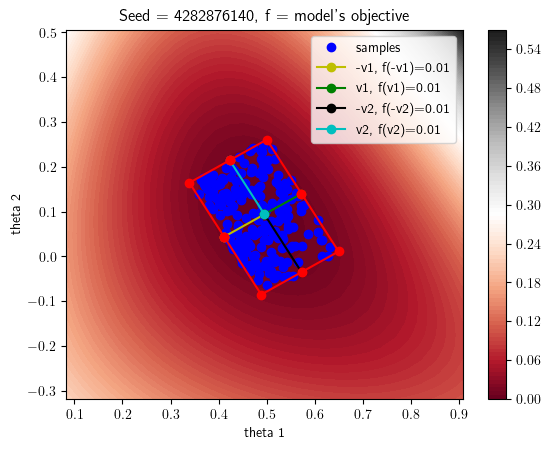
\includegraphics[width=0.49\textwidth]{./latex_files/images/chapter4/ma2_region_1.png}
        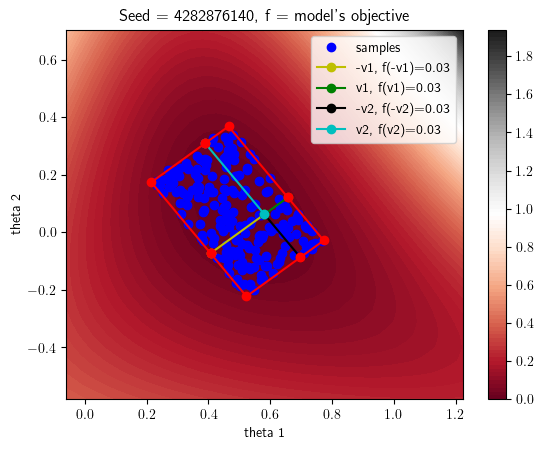
\includegraphics[width=0.49\textwidth]{./latex_files/images/chapter4/ma2_region_1_bo.png}
    \end{center}
  \caption[The acceptance region of a specific deterministic simulator.]{The acceptance region in a specific optimisation problem. In the left figure the region obtained with gradient-based optimiser and in the right one with Bayesian Optimisation.}
  \label{fig:ma2_5}
\end{figure}


\begin{figure}[ht]
  \begin{center}
    \resizebox{.24\columnwidth}{!}{%
      % This file was created with tikzplotlib v0.9.12.
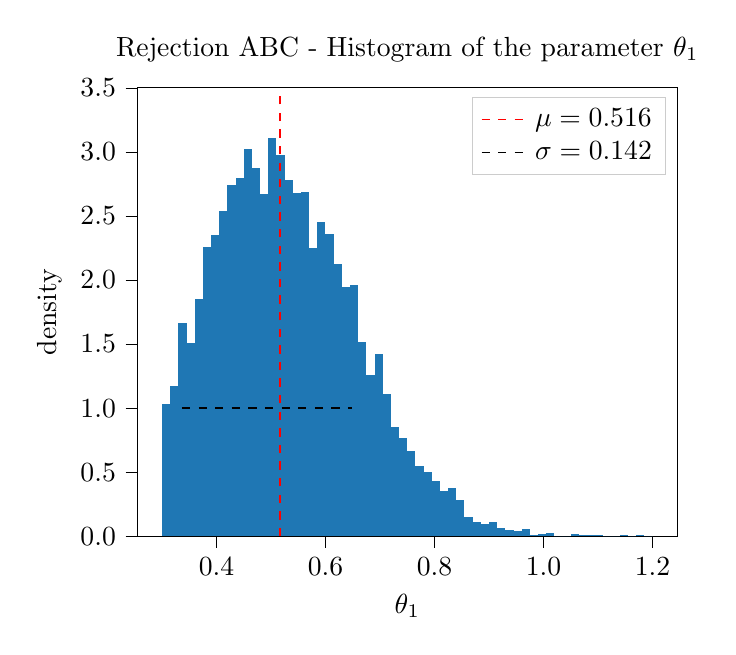
\begin{tikzpicture}

\definecolor{color0}{rgb}{0.12156862745098,0.466666666666667,0.705882352941177}

\begin{axis}[
legend cell align={left},
legend style={fill opacity=0.8, draw opacity=1, text opacity=1, draw=white!80!black},
tick align=outside,
tick pos=left,
title={Rejection ABC - Histogram of the parameter \(\displaystyle \theta_1\)},
x grid style={white!69.0196078431373!black},
xlabel={\(\displaystyle \theta_1\)},
xmin=0.255, xmax=1.245,
xtick style={color=black},
xtick={0.2,0.4,0.6,0.8,1,1.2,1.4},
xticklabels={
  \(\displaystyle {0.2}\),
  \(\displaystyle {0.4}\),
  \(\displaystyle {0.6}\),
  \(\displaystyle {0.8}\),
  \(\displaystyle {1.0}\),
  \(\displaystyle {1.2}\),
  \(\displaystyle {1.4}\)
},
y grid style={white!69.0196078431373!black},
ylabel={density},
ymin=0, ymax=3.5,
ytick style={color=black},
ytick={0,0.5,1,1.5,2,2.5,3,3.5},
yticklabels={
  \(\displaystyle {0.0}\),
  \(\displaystyle {0.5}\),
  \(\displaystyle {1.0}\),
  \(\displaystyle {1.5}\),
  \(\displaystyle {2.0}\),
  \(\displaystyle {2.5}\),
  \(\displaystyle {3.0}\),
  \(\displaystyle {3.5}\)
}
]
\draw[draw=none,fill=color0] (axis cs:0.3,0) rectangle (axis cs:0.315,1.02965548855742);
\draw[draw=none,fill=color0] (axis cs:0.315,0) rectangle (axis cs:0.33,1.17070418562009);
\draw[draw=none,fill=color0] (axis cs:0.33,0) rectangle (axis cs:0.345,1.6643746253394);
\draw[draw=none,fill=color0] (axis cs:0.345,0) rectangle (axis cs:0.36,1.50922105857047);
\draw[draw=none,fill=color0] (axis cs:0.36,0) rectangle (axis cs:0.375,1.85479036637399);
\draw[draw=none,fill=color0] (axis cs:0.375,0) rectangle (axis cs:0.39,2.25677915300258);
\draw[draw=none,fill=color0] (axis cs:0.39,0) rectangle (axis cs:0.405,2.3484608060933);
\draw[draw=none,fill=color0] (axis cs:0.405,0) rectangle (axis cs:0.42,2.53887654712789);
\draw[draw=none,fill=color0] (axis cs:0.42,0) rectangle (axis cs:0.435,2.74339715786876);
\draw[draw=none,fill=color0] (axis cs:0.435,0) rectangle (axis cs:0.45,2.79981663669382);
\draw[draw=none,fill=color0] (axis cs:0.45,0) rectangle (axis cs:0.465,3.02549455199407);
\draw[draw=none,fill=color0] (axis cs:0.465,0) rectangle (axis cs:0.48,2.87739342007828);
\draw[draw=none,fill=color0] (axis cs:0.48,0) rectangle (axis cs:0.495,2.67287280933742);
\draw[draw=none,fill=color0] (axis cs:0.495,0) rectangle (axis cs:0.51,3.11012377023167);
\draw[draw=none,fill=color0] (axis cs:0.51,0) rectangle (axis cs:0.525,2.97612750802216);
\draw[draw=none,fill=color0] (axis cs:0.525,0) rectangle (axis cs:0.54,2.77865933213442);
\draw[draw=none,fill=color0] (axis cs:0.54,0) rectangle (axis cs:0.555,2.67992524419055);
\draw[draw=none,fill=color0] (axis cs:0.555,0) rectangle (axis cs:0.57,2.68697767904369);
\draw[draw=none,fill=color0] (axis cs:0.57,0) rectangle (axis cs:0.585,2.24972671814944);
\draw[draw=none,fill=color0] (axis cs:0.585,0) rectangle (axis cs:0.6,2.45424732889032);
\draw[draw=none,fill=color0] (axis cs:0.6,0) rectangle (axis cs:0.615,2.35551324094642);
\draw[draw=none,fill=color0] (axis cs:0.615,0) rectangle (axis cs:0.63,2.12278289079306);
\draw[draw=none,fill=color0] (axis cs:0.63,0) rectangle (axis cs:0.645,1.9464720194647);
\draw[draw=none,fill=color0] (axis cs:0.645,0) rectangle (axis cs:0.66,1.960576889171);
\draw[draw=none,fill=color0] (axis cs:0.66,0) rectangle (axis cs:0.675,1.5162734934236);
\draw[draw=none,fill=color0] (axis cs:0.675,0) rectangle (axis cs:0.69,1.25533340385768);
\draw[draw=none,fill=color0] (axis cs:0.69,0) rectangle (axis cs:0.705,1.42459184033288);
\draw[draw=none,fill=color0] (axis cs:0.705,0) rectangle (axis cs:0.72,1.10723227194188);
\draw[draw=none,fill=color0] (axis cs:0.72,0) rectangle (axis cs:0.735,0.853344617229104);
\draw[draw=none,fill=color0] (axis cs:0.735,0) rectangle (axis cs:0.75,0.768715398991495);
\draw[draw=none,fill=color0] (axis cs:0.75,0) rectangle (axis cs:0.765,0.66292887619451);
\draw[draw=none,fill=color0] (axis cs:0.765,0) rectangle (axis cs:0.78,0.550089918544377);
\draw[draw=none,fill=color0] (axis cs:0.78,0) rectangle (axis cs:0.795,0.500722874572446);
\draw[draw=none,fill=color0] (axis cs:0.795,0) rectangle (axis cs:0.81,0.430198526041119);
\draw[draw=none,fill=color0] (axis cs:0.81,0) rectangle (axis cs:0.825,0.352621742656649);
\draw[draw=none,fill=color0] (axis cs:0.825,0) rectangle (axis cs:0.84,0.373779047216054);
\draw[draw=none,fill=color0] (axis cs:0.84,0) rectangle (axis cs:0.855,0.282097394125319);
\draw[draw=none,fill=color0] (axis cs:0.855,0) rectangle (axis cs:0.87,0.148101131915795);
\draw[draw=none,fill=color0] (axis cs:0.87,0) rectangle (axis cs:0.885,0.112838957650128);
\draw[draw=none,fill=color0] (axis cs:0.885,0) rectangle (axis cs:0.9,0.0916816530907302);
\draw[draw=none,fill=color0] (axis cs:0.9,0) rectangle (axis cs:0.915,0.112838957650129);
\draw[draw=none,fill=color0] (axis cs:0.915,0) rectangle (axis cs:0.93,0.0634719136781969);
\draw[draw=none,fill=color0] (axis cs:0.93,0) rectangle (axis cs:0.945,0.0493670439719316);
\draw[draw=none,fill=color0] (axis cs:0.945,0) rectangle (axis cs:0.96,0.0423146091187979);
\draw[draw=none,fill=color0] (axis cs:0.96,0) rectangle (axis cs:0.975,0.0564194788250647);
\draw[draw=none,fill=color0] (axis cs:0.975,0) rectangle (axis cs:0.99,0.00705243485313299);
\draw[draw=none,fill=color0] (axis cs:0.99,0) rectangle (axis cs:1.005,0.0141048697062662);
\draw[draw=none,fill=color0] (axis cs:1.005,0) rectangle (axis cs:1.02,0.0282097394125324);
\draw[draw=none,fill=color0] (axis cs:1.02,0) rectangle (axis cs:1.035,0);
\draw[draw=none,fill=color0] (axis cs:1.035,0) rectangle (axis cs:1.05,0);
\draw[draw=none,fill=color0] (axis cs:1.05,0) rectangle (axis cs:1.065,0.014104869706266);
\draw[draw=none,fill=color0] (axis cs:1.065,0) rectangle (axis cs:1.08,0.00705243485313309);
\draw[draw=none,fill=color0] (axis cs:1.08,0) rectangle (axis cs:1.095,0.00705243485313299);
\draw[draw=none,fill=color0] (axis cs:1.095,0) rectangle (axis cs:1.11,0.00705243485313309);
\draw[draw=none,fill=color0] (axis cs:1.11,0) rectangle (axis cs:1.125,0);
\draw[draw=none,fill=color0] (axis cs:1.125,0) rectangle (axis cs:1.14,0);
\draw[draw=none,fill=color0] (axis cs:1.14,0) rectangle (axis cs:1.155,0.00705243485313309);
\draw[draw=none,fill=color0] (axis cs:1.155,0) rectangle (axis cs:1.17,0);
\draw[draw=none,fill=color0] (axis cs:1.17,0) rectangle (axis cs:1.185,0.00705243485313309);
\draw[draw=none,fill=color0] (axis cs:1.185,0) rectangle (axis cs:1.2,0);
\addplot [semithick, red, dashed]
table {%
0.51592730438119 0
0.51592730438119 3.5
};
\addlegendentry{$\mu = 0.516$}
\addplot [semithick, black, dashed]
table {%
0.336596813861936 1
0.648443255776683 1
};
\addlegendentry{$\sigma = 0.142$}
\end{axis}

\end{tikzpicture}

    }
    \resizebox{.24\columnwidth}{!}{%
      % This file was created by tikzplotlib v0.9.9.
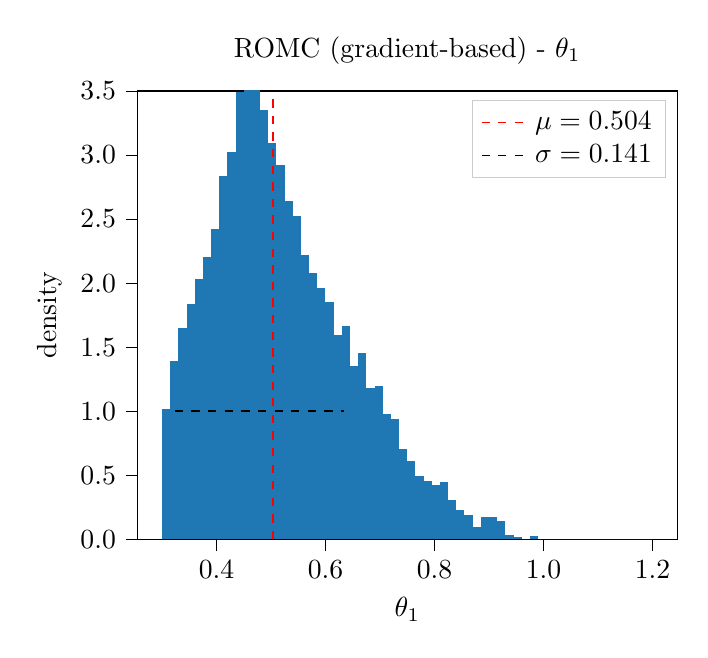
\begin{tikzpicture}

\definecolor{color0}{rgb}{0.12156862745098,0.466666666666667,0.705882352941177}

\begin{axis}[
legend cell align={left},
legend style={fill opacity=0.8, draw opacity=1, text opacity=1, draw=white!80!black},
tick align=outside,
tick pos=left,
title={ROMC (gradient-based) - \(\displaystyle \theta_1\)},
x grid style={white!69.0196078431373!black},
xlabel={\(\displaystyle \theta_1\)},
xmin=0.255, xmax=1.245,
xtick style={color=black},
xtick={0.2,0.4,0.6,0.8,1,1.2,1.4},
xticklabels={
  \(\displaystyle {0.2}\),
  \(\displaystyle {0.4}\),
  \(\displaystyle {0.6}\),
  \(\displaystyle {0.8}\),
  \(\displaystyle {1.0}\),
  \(\displaystyle {1.2}\),
  \(\displaystyle {1.4}\)
},
y grid style={white!69.0196078431373!black},
ylabel={density},
ymin=0, ymax=3.5,
ytick style={color=black},
ytick={0,0.5,1,1.5,2,2.5,3,3.5},
yticklabels={
  \(\displaystyle {0.0}\),
  \(\displaystyle {0.5}\),
  \(\displaystyle {1.0}\),
  \(\displaystyle {1.5}\),
  \(\displaystyle {2.0}\),
  \(\displaystyle {2.5}\),
  \(\displaystyle {3.0}\),
  \(\displaystyle {3.5}\)
}
]
\draw[draw=none,fill=color0] (axis cs:0.3,0) rectangle (axis cs:0.315,1.02018167274615);
\draw[draw=none,fill=color0] (axis cs:0.315,0) rectangle (axis cs:0.33,1.39039538321726);
\draw[draw=none,fill=color0] (axis cs:0.33,0) rectangle (axis cs:0.345,1.64837235793467);
\draw[draw=none,fill=color0] (axis cs:0.345,0) rectangle (axis cs:0.36,1.83766715107148);
\draw[draw=none,fill=color0] (axis cs:0.36,0) rectangle (axis cs:0.375,2.03114988210955);
\draw[draw=none,fill=color0] (axis cs:0.375,0) rectangle (axis cs:0.39,2.20118016090059);
\draw[draw=none,fill=color0] (axis cs:0.39,0) rectangle (axis cs:0.405,2.42565363240795);
\draw[draw=none,fill=color0] (axis cs:0.405,0) rectangle (axis cs:0.42,2.83858430947187);
\draw[draw=none,fill=color0] (axis cs:0.42,0) rectangle (axis cs:0.435,3.02313277298727);
\draw[draw=none,fill=color0] (axis cs:0.435,0) rectangle (axis cs:0.45,3.49050664276752);
\draw[draw=none,fill=color0] (axis cs:0.45,0) rectangle (axis cs:0.465,3.58012851385441);
\draw[draw=none,fill=color0] (axis cs:0.465,0) rectangle (axis cs:0.48,3.63066296452957);
\draw[draw=none,fill=color0] (axis cs:0.48,0) rectangle (axis cs:0.495,3.34895434170502);
\draw[draw=none,fill=color0] (axis cs:0.495,0) rectangle (axis cs:0.51,3.09544450074894);
\draw[draw=none,fill=color0] (axis cs:0.51,0) rectangle (axis cs:0.525,2.92569341781802);
\draw[draw=none,fill=color0] (axis cs:0.525,0) rectangle (axis cs:0.54,2.63923846537203);
\draw[draw=none,fill=color0] (axis cs:0.54,0) rectangle (axis cs:0.555,2.52616414203809);
\draw[draw=none,fill=color0] (axis cs:0.555,0) rectangle (axis cs:0.57,2.21569834562492);
\draw[draw=none,fill=color0] (axis cs:0.57,0) rectangle (axis cs:0.585,2.07749639488345);
\draw[draw=none,fill=color0] (axis cs:0.585,0) rectangle (axis cs:0.6,1.95995493778819);
\draw[draw=none,fill=color0] (axis cs:0.6,0) rectangle (axis cs:0.615,1.85302292337607);
\draw[draw=none,fill=color0] (axis cs:0.615,0) rectangle (axis cs:0.63,1.59560434037885);
\draw[draw=none,fill=color0] (axis cs:0.63,0) rectangle (axis cs:0.645,1.66428652195943);
\draw[draw=none,fill=color0] (axis cs:0.645,0) rectangle (axis cs:0.66,1.3535415296862);
\draw[draw=none,fill=color0] (axis cs:0.66,0) rectangle (axis cs:0.675,1.45042249313527);
\draw[draw=none,fill=color0] (axis cs:0.675,0) rectangle (axis cs:0.69,1.1846280343355);
\draw[draw=none,fill=color0] (axis cs:0.69,0) rectangle (axis cs:0.705,1.19830863147962);
\draw[draw=none,fill=color0] (axis cs:0.705,0) rectangle (axis cs:0.72,0.979977468894081);
\draw[draw=none,fill=color0] (axis cs:0.72,0) rectangle (axis cs:0.735,0.941727636062617);
\draw[draw=none,fill=color0] (axis cs:0.735,0) rectangle (axis cs:0.75,0.705807134291806);
\draw[draw=none,fill=color0] (axis cs:0.75,0) rectangle (axis cs:0.765,0.614789283904501);
\draw[draw=none,fill=color0] (axis cs:0.765,0) rectangle (axis cs:0.78,0.496689435089055);
\draw[draw=none,fill=color0] (axis cs:0.78,0) rectangle (axis cs:0.795,0.456206035376906);
\draw[draw=none,fill=color0] (axis cs:0.795,0) rectangle (axis cs:0.81,0.425773686627776);
\draw[draw=none,fill=color0] (axis cs:0.81,0) rectangle (axis cs:0.825,0.449226138874808);
\draw[draw=none,fill=color0] (axis cs:0.825,0) rectangle (axis cs:0.84,0.309907404693004);
\draw[draw=none,fill=color0] (axis cs:0.84,0) rectangle (axis cs:0.855,0.224752667367446);
\draw[draw=none,fill=color0] (axis cs:0.855,0) rectangle (axis cs:0.87,0.192924339317897);
\draw[draw=none,fill=color0] (axis cs:0.87,0) rectangle (axis cs:0.885,0.0974393551692405);
\draw[draw=none,fill=color0] (axis cs:0.885,0) rectangle (axis cs:0.9,0.176730979433038);
\draw[draw=none,fill=color0] (axis cs:0.9,0) rectangle (axis cs:0.915,0.170309474651111);
\draw[draw=none,fill=color0] (axis cs:0.915,0) rectangle (axis cs:0.93,0.145461043103651);
\draw[draw=none,fill=color0] (axis cs:0.93,0) rectangle (axis cs:0.945,0.0304323487491329);
\draw[draw=none,fill=color0] (axis cs:0.945,0) rectangle (axis cs:0.96,0.0206604936462);
\draw[draw=none,fill=color0] (axis cs:0.96,0) rectangle (axis cs:0.975,0);
\draw[draw=none,fill=color0] (axis cs:0.975,0) rectangle (axis cs:0.99,0.0217772770865351);
\draw[draw=none,fill=color0] (axis cs:0.99,0) rectangle (axis cs:1.005,0);
\draw[draw=none,fill=color0] (axis cs:1.005,0) rectangle (axis cs:1.02,0);
\draw[draw=none,fill=color0] (axis cs:1.02,0) rectangle (axis cs:1.035,0);
\draw[draw=none,fill=color0] (axis cs:1.035,0) rectangle (axis cs:1.05,0);
\draw[draw=none,fill=color0] (axis cs:1.05,0) rectangle (axis cs:1.065,0);
\draw[draw=none,fill=color0] (axis cs:1.065,0) rectangle (axis cs:1.08,0);
\draw[draw=none,fill=color0] (axis cs:1.08,0) rectangle (axis cs:1.095,0);
\draw[draw=none,fill=color0] (axis cs:1.095,0) rectangle (axis cs:1.11,0);
\draw[draw=none,fill=color0] (axis cs:1.11,0) rectangle (axis cs:1.125,0);
\draw[draw=none,fill=color0] (axis cs:1.125,0) rectangle (axis cs:1.14,0);
\draw[draw=none,fill=color0] (axis cs:1.14,0) rectangle (axis cs:1.155,0);
\draw[draw=none,fill=color0] (axis cs:1.155,0) rectangle (axis cs:1.17,0);
\draw[draw=none,fill=color0] (axis cs:1.17,0) rectangle (axis cs:1.185,0);
\draw[draw=none,fill=color0] (axis cs:1.185,0) rectangle (axis cs:1.2,0);
\addplot [semithick, red, dashed]
table {%
0.503688298846839 0
0.503688298846839 3.5
};
\addlegendentry{$\mu = 0.504$}
\addplot [semithick, black, dashed]
table {%
0.323676768279387 1
0.634437489183658 1
};
\addlegendentry{$\sigma = 0.141$}
\end{axis}

\end{tikzpicture}

    }
    \resizebox{.24\columnwidth}{!}{%
      % This file was created by tikzplotlib v0.9.9.
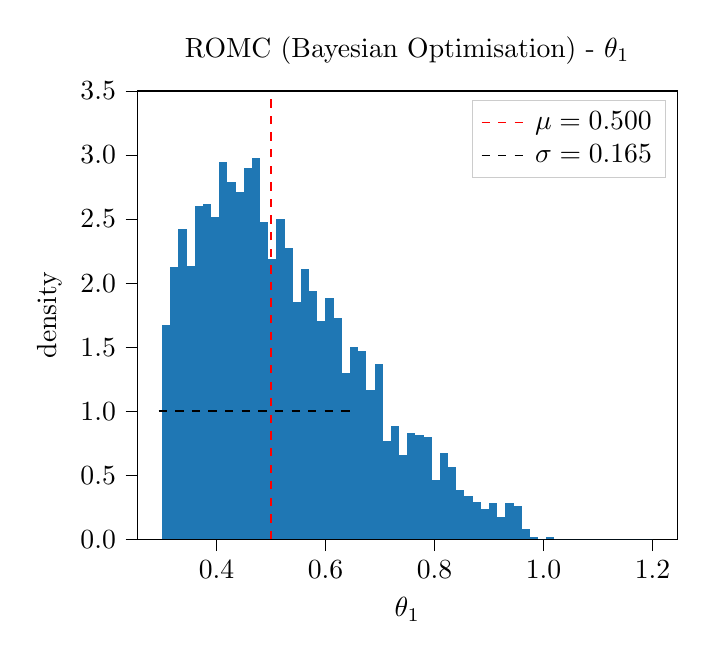
\begin{tikzpicture}

\definecolor{color0}{rgb}{0.12156862745098,0.466666666666667,0.705882352941177}

\begin{axis}[
legend cell align={left},
legend style={fill opacity=0.8, draw opacity=1, text opacity=1, draw=white!80!black},
tick align=outside,
tick pos=left,
title={ROMC (Bayesian Optimisation) - \(\displaystyle \theta_1\)},
x grid style={white!69.0196078431373!black},
xlabel={\(\displaystyle \theta_1\)},
xmin=0.255, xmax=1.245,
xtick style={color=black},
xtick={0.2,0.4,0.6,0.8,1,1.2,1.4},
xticklabels={
  \(\displaystyle {0.2}\),
  \(\displaystyle {0.4}\),
  \(\displaystyle {0.6}\),
  \(\displaystyle {0.8}\),
  \(\displaystyle {1.0}\),
  \(\displaystyle {1.2}\),
  \(\displaystyle {1.4}\)
},
y grid style={white!69.0196078431373!black},
ylabel={density},
ymin=0, ymax=3.5,
ytick style={color=black},
ytick={0,0.5,1,1.5,2,2.5,3,3.5},
yticklabels={
  \(\displaystyle {0.0}\),
  \(\displaystyle {0.5}\),
  \(\displaystyle {1.0}\),
  \(\displaystyle {1.5}\),
  \(\displaystyle {2.0}\),
  \(\displaystyle {2.5}\),
  \(\displaystyle {3.0}\),
  \(\displaystyle {3.5}\)
}
]
\draw[draw=none,fill=color0] (axis cs:0.3,0) rectangle (axis cs:0.315,1.67339010906917);
\draw[draw=none,fill=color0] (axis cs:0.315,0) rectangle (axis cs:0.33,2.12285439456296);
\draw[draw=none,fill=color0] (axis cs:0.33,0) rectangle (axis cs:0.345,2.41994534810638);
\draw[draw=none,fill=color0] (axis cs:0.345,0) rectangle (axis cs:0.36,2.13421448089961);
\draw[draw=none,fill=color0] (axis cs:0.36,0) rectangle (axis cs:0.375,2.60269456308737);
\draw[draw=none,fill=color0] (axis cs:0.375,0) rectangle (axis cs:0.39,2.61479552461991);
\draw[draw=none,fill=color0] (axis cs:0.39,0) rectangle (axis cs:0.405,2.51971654115006);
\draw[draw=none,fill=color0] (axis cs:0.405,0) rectangle (axis cs:0.42,2.94571977877467);
\draw[draw=none,fill=color0] (axis cs:0.42,0) rectangle (axis cs:0.435,2.78840727885186);
\draw[draw=none,fill=color0] (axis cs:0.435,0) rectangle (axis cs:0.45,2.70814579929938);
\draw[draw=none,fill=color0] (axis cs:0.45,0) rectangle (axis cs:0.465,2.89534026545558);
\draw[draw=none,fill=color0] (axis cs:0.465,0) rectangle (axis cs:0.48,2.97807132899427);
\draw[draw=none,fill=color0] (axis cs:0.48,0) rectangle (axis cs:0.495,2.47304140381032);
\draw[draw=none,fill=color0] (axis cs:0.495,0) rectangle (axis cs:0.51,2.18508791101595);
\draw[draw=none,fill=color0] (axis cs:0.51,0) rectangle (axis cs:0.525,2.50193553644923);
\draw[draw=none,fill=color0] (axis cs:0.525,0) rectangle (axis cs:0.54,2.27646251850645);
\draw[draw=none,fill=color0] (axis cs:0.54,0) rectangle (axis cs:0.555,1.84996536408459);
\draw[draw=none,fill=color0] (axis cs:0.555,0) rectangle (axis cs:0.57,2.10951864103732);
\draw[draw=none,fill=color0] (axis cs:0.57,0) rectangle (axis cs:0.585,1.94010517958197);
\draw[draw=none,fill=color0] (axis cs:0.585,0) rectangle (axis cs:0.6,1.70154336651221);
\draw[draw=none,fill=color0] (axis cs:0.6,0) rectangle (axis cs:0.615,1.88058820551382);
\draw[draw=none,fill=color0] (axis cs:0.615,0) rectangle (axis cs:0.63,1.72549833117864);
\draw[draw=none,fill=color0] (axis cs:0.63,0) rectangle (axis cs:0.645,1.29579071757466);
\draw[draw=none,fill=color0] (axis cs:0.645,0) rectangle (axis cs:0.66,1.50076618843174);
\draw[draw=none,fill=color0] (axis cs:0.66,0) rectangle (axis cs:0.675,1.46940247180661);
\draw[draw=none,fill=color0] (axis cs:0.675,0) rectangle (axis cs:0.69,1.16860714228384);
\draw[draw=none,fill=color0] (axis cs:0.69,0) rectangle (axis cs:0.705,1.37012519556019);
\draw[draw=none,fill=color0] (axis cs:0.705,0) rectangle (axis cs:0.72,0.767793661318775);
\draw[draw=none,fill=color0] (axis cs:0.72,0) rectangle (axis cs:0.735,0.885098900664694);
\draw[draw=none,fill=color0] (axis cs:0.735,0) rectangle (axis cs:0.75,0.65715629873569);
\draw[draw=none,fill=color0] (axis cs:0.75,0) rectangle (axis cs:0.765,0.82731063538692);
\draw[draw=none,fill=color0] (axis cs:0.765,0) rectangle (axis cs:0.78,0.813727923462651);
\draw[draw=none,fill=color0] (axis cs:0.78,0) rectangle (axis cs:0.795,0.801873920328749);
\draw[draw=none,fill=color0] (axis cs:0.795,0) rectangle (axis cs:0.81,0.459095663040085);
\draw[draw=none,fill=color0] (axis cs:0.81,0) rectangle (axis cs:0.825,0.672961636247559);
\draw[draw=none,fill=color0] (axis cs:0.825,0) rectangle (axis cs:0.84,0.561583398468614);
\draw[draw=none,fill=color0] (axis cs:0.84,0) rectangle (axis cs:0.855,0.382538559466961);
\draw[draw=none,fill=color0] (axis cs:0.855,0) rectangle (axis cs:0.87,0.340555631701063);
\draw[draw=none,fill=color0] (axis cs:0.87,0) rectangle (axis cs:0.885,0.294127452759942);
\draw[draw=none,fill=color0] (axis cs:0.885,0) rectangle (axis cs:0.9,0.239055729867026);
\draw[draw=none,fill=color0] (axis cs:0.9,0) rectangle (axis cs:0.915,0.283755200017783);
\draw[draw=none,fill=color0] (axis cs:0.915,0) rectangle (axis cs:0.93,0.176575255015415);
\draw[draw=none,fill=color0] (axis cs:0.93,0) rectangle (axis cs:0.945,0.283261283220537);
\draw[draw=none,fill=color0] (axis cs:0.945,0) rectangle (axis cs:0.96,0.258071526560991);
\draw[draw=none,fill=color0] (axis cs:0.96,0) rectangle (axis cs:0.975,0.0775449371676099);
\draw[draw=none,fill=color0] (axis cs:0.975,0) rectangle (axis cs:0.99,0.0155583791132463);
\draw[draw=none,fill=color0] (axis cs:0.99,0) rectangle (axis cs:1.005,0);
\draw[draw=none,fill=color0] (axis cs:1.005,0) rectangle (axis cs:1.02,0.0172870879036073);
\draw[draw=none,fill=color0] (axis cs:1.02,0) rectangle (axis cs:1.035,0);
\draw[draw=none,fill=color0] (axis cs:1.035,0) rectangle (axis cs:1.05,0);
\draw[draw=none,fill=color0] (axis cs:1.05,0) rectangle (axis cs:1.065,0);
\draw[draw=none,fill=color0] (axis cs:1.065,0) rectangle (axis cs:1.08,0);
\draw[draw=none,fill=color0] (axis cs:1.08,0) rectangle (axis cs:1.095,0);
\draw[draw=none,fill=color0] (axis cs:1.095,0) rectangle (axis cs:1.11,0);
\draw[draw=none,fill=color0] (axis cs:1.11,0) rectangle (axis cs:1.125,0);
\draw[draw=none,fill=color0] (axis cs:1.125,0) rectangle (axis cs:1.14,0);
\draw[draw=none,fill=color0] (axis cs:1.14,0) rectangle (axis cs:1.155,0);
\draw[draw=none,fill=color0] (axis cs:1.155,0) rectangle (axis cs:1.17,0);
\draw[draw=none,fill=color0] (axis cs:1.17,0) rectangle (axis cs:1.185,0);
\draw[draw=none,fill=color0] (axis cs:1.185,0) rectangle (axis cs:1.2,0);
\addplot [semithick, red, dashed]
table {%
0.500240536632723 0
0.500240536632723 3.5
};
\addlegendentry{$\mu = 0.500$}
\addplot [semithick, black, dashed]
table {%
0.293929386789429 1
0.656599793802562 1
};
\addlegendentry{$\sigma = 0.165$}
\end{axis}

\end{tikzpicture}

    }
    \resizebox{.24\columnwidth}{!}{%
      % This file was created with tikzplotlib v0.9.12.
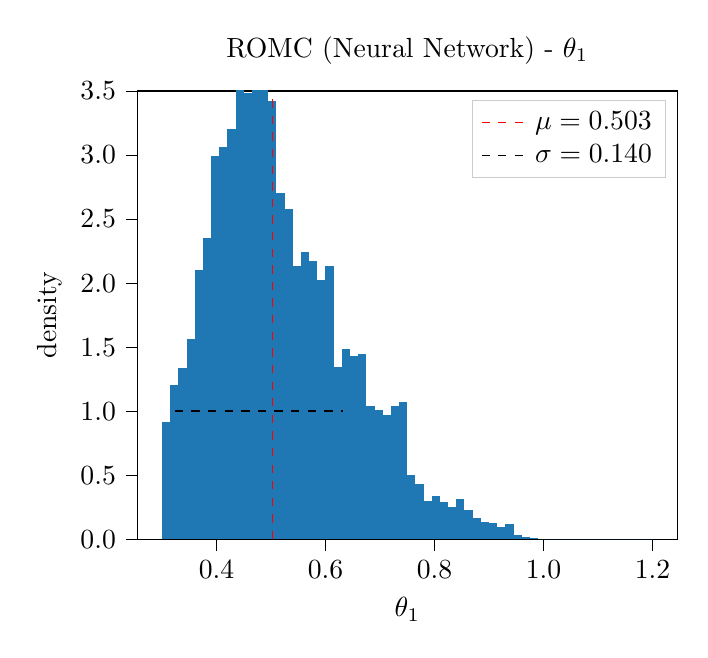
\begin{tikzpicture}

\definecolor{color0}{rgb}{0.12156862745098,0.466666666666667,0.705882352941177}

\begin{axis}[
legend cell align={left},
legend style={fill opacity=0.8, draw opacity=1, text opacity=1, draw=white!80!black},
tick align=outside,
tick pos=left,
title={ROMC (Neural Network) - \(\displaystyle \theta_1\)},
x grid style={white!69.0196078431373!black},
xlabel={\(\displaystyle \theta_1\)},
xmin=0.255, xmax=1.245,
xtick style={color=black},
xtick={0.2,0.4,0.6,0.8,1,1.2,1.4},
xticklabels={
  \(\displaystyle {0.2}\),
  \(\displaystyle {0.4}\),
  \(\displaystyle {0.6}\),
  \(\displaystyle {0.8}\),
  \(\displaystyle {1.0}\),
  \(\displaystyle {1.2}\),
  \(\displaystyle {1.4}\)
},
y grid style={white!69.0196078431373!black},
ylabel={density},
ymin=0, ymax=3.5,
ytick style={color=black},
ytick={0,0.5,1,1.5,2,2.5,3,3.5},
yticklabels={
  \(\displaystyle {0.0}\),
  \(\displaystyle {0.5}\),
  \(\displaystyle {1.0}\),
  \(\displaystyle {1.5}\),
  \(\displaystyle {2.0}\),
  \(\displaystyle {2.5}\),
  \(\displaystyle {3.0}\),
  \(\displaystyle {3.5}\)
}
]
\draw[draw=none,fill=color0] (axis cs:0.3,0) rectangle (axis cs:0.315,0.918657455133441);
\draw[draw=none,fill=color0] (axis cs:0.315,0) rectangle (axis cs:0.33,1.20251419656731);
\draw[draw=none,fill=color0] (axis cs:0.33,0) rectangle (axis cs:0.345,1.33742778487049);
\draw[draw=none,fill=color0] (axis cs:0.345,0) rectangle (axis cs:0.36,1.56194622164953);
\draw[draw=none,fill=color0] (axis cs:0.36,0) rectangle (axis cs:0.375,2.10132928493464);
\draw[draw=none,fill=color0] (axis cs:0.375,0) rectangle (axis cs:0.39,2.35262182295654);
\draw[draw=none,fill=color0] (axis cs:0.39,0) rectangle (axis cs:0.405,2.99077324408847);
\draw[draw=none,fill=color0] (axis cs:0.405,0) rectangle (axis cs:0.42,3.06195916743878);
\draw[draw=none,fill=color0] (axis cs:0.42,0) rectangle (axis cs:0.435,3.20534143070652);
\draw[draw=none,fill=color0] (axis cs:0.435,0) rectangle (axis cs:0.45,3.54249833812081);
\draw[draw=none,fill=color0] (axis cs:0.45,0) rectangle (axis cs:0.465,3.48746191660371);
\draw[draw=none,fill=color0] (axis cs:0.465,0) rectangle (axis cs:0.48,3.64921604449934);
\draw[draw=none,fill=color0] (axis cs:0.48,0) rectangle (axis cs:0.495,3.65237906359403);
\draw[draw=none,fill=color0] (axis cs:0.495,0) rectangle (axis cs:0.51,3.41841807637564);
\draw[draw=none,fill=color0] (axis cs:0.51,0) rectangle (axis cs:0.525,2.70295622336452);
\draw[draw=none,fill=color0] (axis cs:0.525,0) rectangle (axis cs:0.54,2.57664640133676);
\draw[draw=none,fill=color0] (axis cs:0.54,0) rectangle (axis cs:0.555,2.13473725538676);
\draw[draw=none,fill=color0] (axis cs:0.555,0) rectangle (axis cs:0.57,2.24111391157059);
\draw[draw=none,fill=color0] (axis cs:0.57,0) rectangle (axis cs:0.585,2.17436219440432);
\draw[draw=none,fill=color0] (axis cs:0.585,0) rectangle (axis cs:0.6,2.02392362475434);
\draw[draw=none,fill=color0] (axis cs:0.6,0) rectangle (axis cs:0.615,2.1307420959631);
\draw[draw=none,fill=color0] (axis cs:0.615,0) rectangle (axis cs:0.63,1.34480742455423);
\draw[draw=none,fill=color0] (axis cs:0.63,0) rectangle (axis cs:0.645,1.48585437983289);
\draw[draw=none,fill=color0] (axis cs:0.645,0) rectangle (axis cs:0.66,1.43000242757426);
\draw[draw=none,fill=color0] (axis cs:0.66,0) rectangle (axis cs:0.675,1.44793856735925);
\draw[draw=none,fill=color0] (axis cs:0.675,0) rectangle (axis cs:0.69,1.04402163798497);
\draw[draw=none,fill=color0] (axis cs:0.69,0) rectangle (axis cs:0.705,1.00795945546565);
\draw[draw=none,fill=color0] (axis cs:0.705,0) rectangle (axis cs:0.72,0.973472415485145);
\draw[draw=none,fill=color0] (axis cs:0.72,0) rectangle (axis cs:0.735,1.03878684968805);
\draw[draw=none,fill=color0] (axis cs:0.735,0) rectangle (axis cs:0.75,1.07033952922709);
\draw[draw=none,fill=color0] (axis cs:0.75,0) rectangle (axis cs:0.765,0.499611406245489);
\draw[draw=none,fill=color0] (axis cs:0.765,0) rectangle (axis cs:0.78,0.427526350563684);
\draw[draw=none,fill=color0] (axis cs:0.78,0) rectangle (axis cs:0.795,0.301712601546415);
\draw[draw=none,fill=color0] (axis cs:0.795,0) rectangle (axis cs:0.81,0.33618635385698);
\draw[draw=none,fill=color0] (axis cs:0.81,0) rectangle (axis cs:0.825,0.291403030644556);
\draw[draw=none,fill=color0] (axis cs:0.825,0) rectangle (axis cs:0.84,0.251052806310352);
\draw[draw=none,fill=color0] (axis cs:0.84,0) rectangle (axis cs:0.855,0.313679809271219);
\draw[draw=none,fill=color0] (axis cs:0.855,0) rectangle (axis cs:0.87,0.230501210162083);
\draw[draw=none,fill=color0] (axis cs:0.87,0) rectangle (axis cs:0.885,0.16371073729186);
\draw[draw=none,fill=color0] (axis cs:0.885,0) rectangle (axis cs:0.9,0.133740397779522);
\draw[draw=none,fill=color0] (axis cs:0.9,0) rectangle (axis cs:0.915,0.128624644858993);
\draw[draw=none,fill=color0] (axis cs:0.915,0) rectangle (axis cs:0.93,0.097498278063311);
\draw[draw=none,fill=color0] (axis cs:0.93,0) rectangle (axis cs:0.945,0.119954440233943);
\draw[draw=none,fill=color0] (axis cs:0.945,0) rectangle (axis cs:0.96,0.0362421197162086);
\draw[draw=none,fill=color0] (axis cs:0.96,0) rectangle (axis cs:0.975,0.0137859575455791);
\draw[draw=none,fill=color0] (axis cs:0.975,0) rectangle (axis cs:0.99,0.0112280810853149);
\draw[draw=none,fill=color0] (axis cs:0.99,0) rectangle (axis cs:1.005,0);
\draw[draw=none,fill=color0] (axis cs:1.005,0) rectangle (axis cs:1.02,0);
\draw[draw=none,fill=color0] (axis cs:1.02,0) rectangle (axis cs:1.035,0);
\draw[draw=none,fill=color0] (axis cs:1.035,0) rectangle (axis cs:1.05,0);
\draw[draw=none,fill=color0] (axis cs:1.05,0) rectangle (axis cs:1.065,0);
\draw[draw=none,fill=color0] (axis cs:1.065,0) rectangle (axis cs:1.08,0);
\draw[draw=none,fill=color0] (axis cs:1.08,0) rectangle (axis cs:1.095,0);
\draw[draw=none,fill=color0] (axis cs:1.095,0) rectangle (axis cs:1.11,0);
\draw[draw=none,fill=color0] (axis cs:1.11,0) rectangle (axis cs:1.125,0);
\draw[draw=none,fill=color0] (axis cs:1.125,0) rectangle (axis cs:1.14,0);
\draw[draw=none,fill=color0] (axis cs:1.14,0) rectangle (axis cs:1.155,0);
\draw[draw=none,fill=color0] (axis cs:1.155,0) rectangle (axis cs:1.17,0);
\draw[draw=none,fill=color0] (axis cs:1.17,0) rectangle (axis cs:1.185,0);
\draw[draw=none,fill=color0] (axis cs:1.185,0) rectangle (axis cs:1.2,0);
\addplot [semithick, red, dashed]
table {%
0.502656907372089 0
0.502656907372089 3.5
};
\addlegendentry{$\mu = 0.503$}
\addplot [semithick, black, dashed]
table {%
0.32355294654317 1
0.632292249675427 1
};
\addlegendentry{$\sigma = 0.140$}
\end{axis}

\end{tikzpicture}

    }\\
    \resizebox{.24\columnwidth}{!}{%
      % This file was created with tikzplotlib v0.9.12.
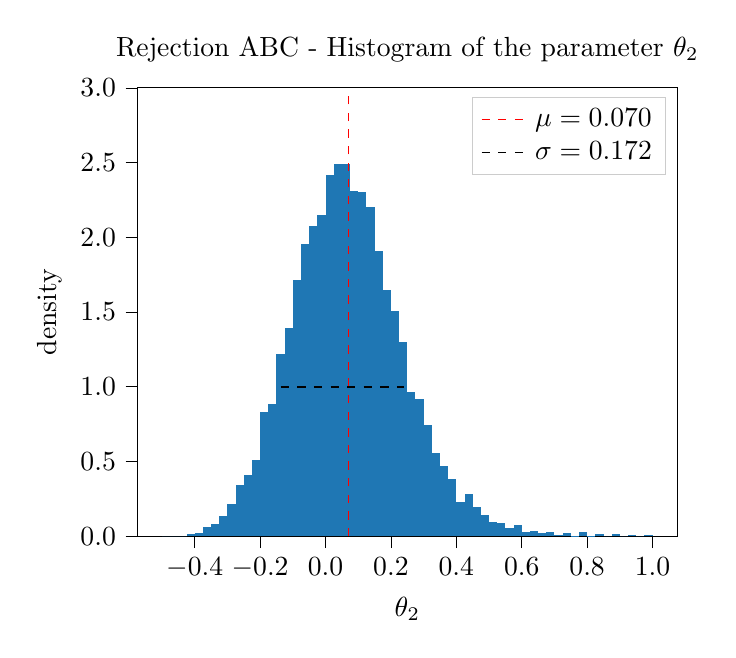
\begin{tikzpicture}

\definecolor{color0}{rgb}{0.12156862745098,0.466666666666667,0.705882352941177}

\begin{axis}[
legend cell align={left},
legend style={fill opacity=0.8, draw opacity=1, text opacity=1, draw=white!80!black},
tick align=outside,
tick pos=left,
title={Rejection ABC - Histogram of the parameter \(\displaystyle \theta_2\)},
x grid style={white!69.0196078431373!black},
xlabel={\(\displaystyle \theta_2\)},
xmin=-0.575, xmax=1.075,
xtick style={color=black},
xtick={-0.6,-0.4,-0.2,0,0.2,0.4,0.6,0.8,1,1.2},
xticklabels={
  \(\displaystyle {\ensuremath{-}0.6}\),
  \(\displaystyle {\ensuremath{-}0.4}\),
  \(\displaystyle {\ensuremath{-}0.2}\),
  \(\displaystyle {0.0}\),
  \(\displaystyle {0.2}\),
  \(\displaystyle {0.4}\),
  \(\displaystyle {0.6}\),
  \(\displaystyle {0.8}\),
  \(\displaystyle {1.0}\),
  \(\displaystyle {1.2}\)
},
y grid style={white!69.0196078431373!black},
ylabel={density},
ymin=0, ymax=3,
ytick style={color=black},
ytick={0,0.5,1,1.5,2,2.5,3},
yticklabels={
  \(\displaystyle {0.0}\),
  \(\displaystyle {0.5}\),
  \(\displaystyle {1.0}\),
  \(\displaystyle {1.5}\),
  \(\displaystyle {2.0}\),
  \(\displaystyle {2.5}\),
  \(\displaystyle {3.0}\)
}
]
\draw[draw=none,fill=color0] (axis cs:-0.5,0) rectangle (axis cs:-0.475,0);
\draw[draw=none,fill=color0] (axis cs:-0.475,0) rectangle (axis cs:-0.45,0);
\draw[draw=none,fill=color0] (axis cs:-0.45,0) rectangle (axis cs:-0.425,0);
\draw[draw=none,fill=color0] (axis cs:-0.425,0) rectangle (axis cs:-0.4,0.016001600160016);
\draw[draw=none,fill=color0] (axis cs:-0.4,0) rectangle (axis cs:-0.375,0.02000200020002);
\draw[draw=none,fill=color0] (axis cs:-0.375,0) rectangle (axis cs:-0.35,0.0600060006000599);
\draw[draw=none,fill=color0] (axis cs:-0.35,0) rectangle (axis cs:-0.325,0.0800080008000799);
\draw[draw=none,fill=color0] (axis cs:-0.325,0) rectangle (axis cs:-0.3,0.132013201320132);
\draw[draw=none,fill=color0] (axis cs:-0.3,0) rectangle (axis cs:-0.275,0.216021602160216);
\draw[draw=none,fill=color0] (axis cs:-0.275,0) rectangle (axis cs:-0.25,0.344034403440344);
\draw[draw=none,fill=color0] (axis cs:-0.25,0) rectangle (axis cs:-0.225,0.412041204120412);
\draw[draw=none,fill=color0] (axis cs:-0.225,0) rectangle (axis cs:-0.2,0.508050805080508);
\draw[draw=none,fill=color0] (axis cs:-0.2,0) rectangle (axis cs:-0.175,0.832083208320833);
\draw[draw=none,fill=color0] (axis cs:-0.175,0) rectangle (axis cs:-0.15,0.884088408840883);
\draw[draw=none,fill=color0] (axis cs:-0.15,0) rectangle (axis cs:-0.125,1.21612161216122);
\draw[draw=none,fill=color0] (axis cs:-0.125,0) rectangle (axis cs:-0.1,1.39213921392139);
\draw[draw=none,fill=color0] (axis cs:-0.1,0) rectangle (axis cs:-0.075,1.71217121712171);
\draw[draw=none,fill=color0] (axis cs:-0.075,0) rectangle (axis cs:-0.05,1.95219521952195);
\draw[draw=none,fill=color0] (axis cs:-0.05,0) rectangle (axis cs:-0.025,2.07620762076207);
\draw[draw=none,fill=color0] (axis cs:-0.025,0) rectangle (axis cs:0,2.15221522152216);
\draw[draw=none,fill=color0] (axis cs:0,0) rectangle (axis cs:0.025,2.41624162416241);
\draw[draw=none,fill=color0] (axis cs:0.025,0) rectangle (axis cs:0.05,2.49224922492249);
\draw[draw=none,fill=color0] (axis cs:0.05,0) rectangle (axis cs:0.0750000000000001,2.48824882488249);
\draw[draw=none,fill=color0] (axis cs:0.0750000000000001,0) rectangle (axis cs:0.1,2.30823082308231);
\draw[draw=none,fill=color0] (axis cs:0.1,0) rectangle (axis cs:0.125,2.30423042304231);
\draw[draw=none,fill=color0] (axis cs:0.125,0) rectangle (axis cs:0.15,2.2042204220422);
\draw[draw=none,fill=color0] (axis cs:0.15,0) rectangle (axis cs:0.175,1.90819081908191);
\draw[draw=none,fill=color0] (axis cs:0.175,0) rectangle (axis cs:0.2,1.64816481648165);
\draw[draw=none,fill=color0] (axis cs:0.2,0) rectangle (axis cs:0.225,1.50815081508151);
\draw[draw=none,fill=color0] (axis cs:0.225,0) rectangle (axis cs:0.25,1.3001300130013);
\draw[draw=none,fill=color0] (axis cs:0.25,0) rectangle (axis cs:0.275,0.964096409640963);
\draw[draw=none,fill=color0] (axis cs:0.275,0) rectangle (axis cs:0.3,0.920092009200919);
\draw[draw=none,fill=color0] (axis cs:0.3,0) rectangle (axis cs:0.325,0.744074407440743);
\draw[draw=none,fill=color0] (axis cs:0.325,0) rectangle (axis cs:0.35,0.556055605560556);
\draw[draw=none,fill=color0] (axis cs:0.35,0) rectangle (axis cs:0.375,0.472047204720474);
\draw[draw=none,fill=color0] (axis cs:0.375,0) rectangle (axis cs:0.4,0.38003800380038);
\draw[draw=none,fill=color0] (axis cs:0.4,0) rectangle (axis cs:0.425,0.228022802280228);
\draw[draw=none,fill=color0] (axis cs:0.425,0) rectangle (axis cs:0.45,0.28002800280028);
\draw[draw=none,fill=color0] (axis cs:0.45,0) rectangle (axis cs:0.475,0.192019201920192);
\draw[draw=none,fill=color0] (axis cs:0.475,0) rectangle (axis cs:0.5,0.140014001400141);
\draw[draw=none,fill=color0] (axis cs:0.5,0) rectangle (axis cs:0.525,0.0960096009600955);
\draw[draw=none,fill=color0] (axis cs:0.525,0) rectangle (axis cs:0.55,0.0880088008800883);
\draw[draw=none,fill=color0] (axis cs:0.55,0) rectangle (axis cs:0.575,0.0560056005600562);
\draw[draw=none,fill=color0] (axis cs:0.575,0) rectangle (axis cs:0.6,0.0760076007600756);
\draw[draw=none,fill=color0] (axis cs:0.6,0) rectangle (axis cs:0.625,0.0280028002800281);
\draw[draw=none,fill=color0] (axis cs:0.625,0) rectangle (axis cs:0.65,0.0360036003600358);
\draw[draw=none,fill=color0] (axis cs:0.65,0) rectangle (axis cs:0.675,0.0240024002400241);
\draw[draw=none,fill=color0] (axis cs:0.675,0) rectangle (axis cs:0.7,0.0280028002800279);
\draw[draw=none,fill=color0] (axis cs:0.7,0) rectangle (axis cs:0.725,0.00800080008000803);
\draw[draw=none,fill=color0] (axis cs:0.725,0) rectangle (axis cs:0.75,0.0200020002000201);
\draw[draw=none,fill=color0] (axis cs:0.75,0) rectangle (axis cs:0.775,0.00400040004000398);
\draw[draw=none,fill=color0] (axis cs:0.775,0) rectangle (axis cs:0.8,0.0280028002800281);
\draw[draw=none,fill=color0] (axis cs:0.8,0) rectangle (axis cs:0.825,0.00400040004000398);
\draw[draw=none,fill=color0] (axis cs:0.825,0) rectangle (axis cs:0.85,0.0160016001600161);
\draw[draw=none,fill=color0] (axis cs:0.85,0) rectangle (axis cs:0.875,0);
\draw[draw=none,fill=color0] (axis cs:0.875,0) rectangle (axis cs:0.9,0.0120012001200119);
\draw[draw=none,fill=color0] (axis cs:0.9,0) rectangle (axis cs:0.925,0);
\draw[draw=none,fill=color0] (axis cs:0.925,0) rectangle (axis cs:0.95,0.00800080008000796);
\draw[draw=none,fill=color0] (axis cs:0.95,0) rectangle (axis cs:0.975,0);
\draw[draw=none,fill=color0] (axis cs:0.975,0) rectangle (axis cs:1,0.00800080008000803);
\addplot [semithick, red, dashed]
table {%
0.0698328247281109 0
0.0698328247281109 3
};
\addlegendentry{$\mu = 0.070$}
\addplot [semithick, black, dashed]
table {%
-0.136927686891309 1
0.240559901293153 1
};
\addlegendentry{$\sigma = 0.172$}
\end{axis}

\end{tikzpicture}

    }
    \resizebox{.24\columnwidth}{!}{%
      % This file was created with tikzplotlib v0.9.12.
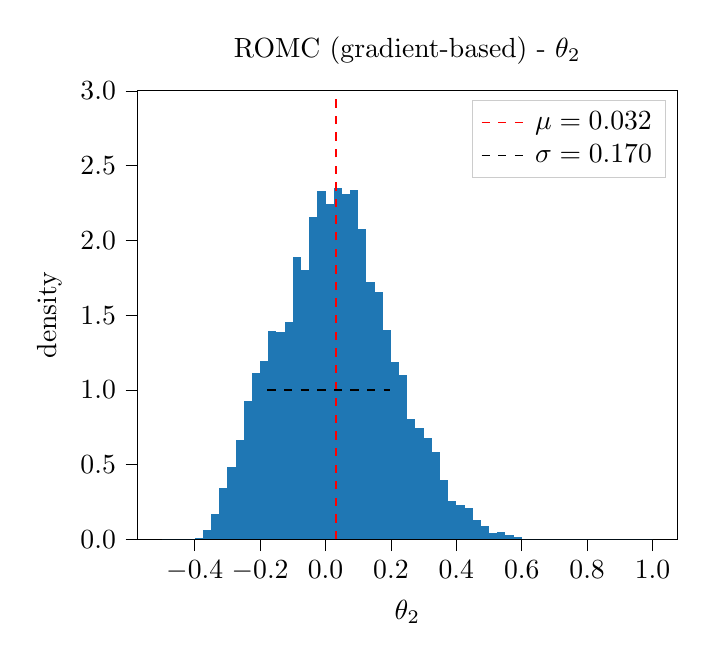
\begin{tikzpicture}

\definecolor{color0}{rgb}{0.12156862745098,0.466666666666667,0.705882352941177}

\begin{axis}[
legend cell align={left},
legend style={fill opacity=0.8, draw opacity=1, text opacity=1, draw=white!80!black},
tick align=outside,
tick pos=left,
title={ROMC (gradient-based) - \(\displaystyle \theta_2\)},
x grid style={white!69.0196078431373!black},
xlabel={\(\displaystyle \theta_2\)},
xmin=-0.575, xmax=1.075,
xtick style={color=black},
xtick={-0.6,-0.4,-0.2,0,0.2,0.4,0.6,0.8,1,1.2},
xticklabels={
  \(\displaystyle {\ensuremath{-}0.6}\),
  \(\displaystyle {\ensuremath{-}0.4}\),
  \(\displaystyle {\ensuremath{-}0.2}\),
  \(\displaystyle {0.0}\),
  \(\displaystyle {0.2}\),
  \(\displaystyle {0.4}\),
  \(\displaystyle {0.6}\),
  \(\displaystyle {0.8}\),
  \(\displaystyle {1.0}\),
  \(\displaystyle {1.2}\)
},
y grid style={white!69.0196078431373!black},
ylabel={density},
ymin=0, ymax=3,
ytick style={color=black},
ytick={0,0.5,1,1.5,2,2.5,3},
yticklabels={
  \(\displaystyle {0.0}\),
  \(\displaystyle {0.5}\),
  \(\displaystyle {1.0}\),
  \(\displaystyle {1.5}\),
  \(\displaystyle {2.0}\),
  \(\displaystyle {2.5}\),
  \(\displaystyle {3.0}\)
}
]
\draw[draw=none,fill=color0] (axis cs:-0.5,0) rectangle (axis cs:-0.475,0);
\draw[draw=none,fill=color0] (axis cs:-0.475,0) rectangle (axis cs:-0.45,0);
\draw[draw=none,fill=color0] (axis cs:-0.45,0) rectangle (axis cs:-0.425,0);
\draw[draw=none,fill=color0] (axis cs:-0.425,0) rectangle (axis cs:-0.4,0);
\draw[draw=none,fill=color0] (axis cs:-0.4,0) rectangle (axis cs:-0.375,0.00551481774368941);
\draw[draw=none,fill=color0] (axis cs:-0.375,0) rectangle (axis cs:-0.35,0.0605814218347914);
\draw[draw=none,fill=color0] (axis cs:-0.35,0) rectangle (axis cs:-0.325,0.168699423699822);
\draw[draw=none,fill=color0] (axis cs:-0.325,0) rectangle (axis cs:-0.3,0.340262186728983);
\draw[draw=none,fill=color0] (axis cs:-0.3,0) rectangle (axis cs:-0.275,0.48172967019454);
\draw[draw=none,fill=color0] (axis cs:-0.275,0) rectangle (axis cs:-0.25,0.661723210849365);
\draw[draw=none,fill=color0] (axis cs:-0.25,0) rectangle (axis cs:-0.225,0.926167683238105);
\draw[draw=none,fill=color0] (axis cs:-0.225,0) rectangle (axis cs:-0.2,1.1131441320768);
\draw[draw=none,fill=color0] (axis cs:-0.2,0) rectangle (axis cs:-0.175,1.19038558853121);
\draw[draw=none,fill=color0] (axis cs:-0.175,0) rectangle (axis cs:-0.15,1.39560413532974);
\draw[draw=none,fill=color0] (axis cs:-0.15,0) rectangle (axis cs:-0.125,1.38890799766854);
\draw[draw=none,fill=color0] (axis cs:-0.125,0) rectangle (axis cs:-0.1,1.45486223069012);
\draw[draw=none,fill=color0] (axis cs:-0.1,0) rectangle (axis cs:-0.075,1.89014334843844);
\draw[draw=none,fill=color0] (axis cs:-0.075,0) rectangle (axis cs:-0.05,1.80399178478282);
\draw[draw=none,fill=color0] (axis cs:-0.05,0) rectangle (axis cs:-0.025,2.15561058973456);
\draw[draw=none,fill=color0] (axis cs:-0.025,0) rectangle (axis cs:0,2.33061276076321);
\draw[draw=none,fill=color0] (axis cs:0,0) rectangle (axis cs:0.025,2.24024442959031);
\draw[draw=none,fill=color0] (axis cs:0.025,0) rectangle (axis cs:0.05,2.34890403251458);
\draw[draw=none,fill=color0] (axis cs:0.05,0) rectangle (axis cs:0.0750000000000001,2.31095726097247);
\draw[draw=none,fill=color0] (axis cs:0.0750000000000001,0) rectangle (axis cs:0.1,2.33900171768764);
\draw[draw=none,fill=color0] (axis cs:0.1,0) rectangle (axis cs:0.125,2.07598627244674);
\draw[draw=none,fill=color0] (axis cs:0.125,0) rectangle (axis cs:0.15,1.71987564844275);
\draw[draw=none,fill=color0] (axis cs:0.15,0) rectangle (axis cs:0.175,1.65165022964706);
\draw[draw=none,fill=color0] (axis cs:0.175,0) rectangle (axis cs:0.2,1.40256222683377);
\draw[draw=none,fill=color0] (axis cs:0.2,0) rectangle (axis cs:0.225,1.18758980571923);
\draw[draw=none,fill=color0] (axis cs:0.225,0) rectangle (axis cs:0.25,1.0980208933351);
\draw[draw=none,fill=color0] (axis cs:0.25,0) rectangle (axis cs:0.275,0.803715750920935);
\draw[draw=none,fill=color0] (axis cs:0.275,0) rectangle (axis cs:0.3,0.742179116696122);
\draw[draw=none,fill=color0] (axis cs:0.3,0) rectangle (axis cs:0.325,0.678702875114039);
\draw[draw=none,fill=color0] (axis cs:0.325,0) rectangle (axis cs:0.35,0.583516431505742);
\draw[draw=none,fill=color0] (axis cs:0.35,0) rectangle (axis cs:0.375,0.398341719580722);
\draw[draw=none,fill=color0] (axis cs:0.375,0) rectangle (axis cs:0.4,0.257727424376927);
\draw[draw=none,fill=color0] (axis cs:0.4,0) rectangle (axis cs:0.425,0.229546935490747);
\draw[draw=none,fill=color0] (axis cs:0.425,0) rectangle (axis cs:0.45,0.210112717761985);
\draw[draw=none,fill=color0] (axis cs:0.45,0) rectangle (axis cs:0.475,0.129179090828181);
\draw[draw=none,fill=color0] (axis cs:0.475,0) rectangle (axis cs:0.5,0.0899034779939157);
\draw[draw=none,fill=color0] (axis cs:0.5,0) rectangle (axis cs:0.525,0.0431810229330879);
\draw[draw=none,fill=color0] (axis cs:0.525,0) rectangle (axis cs:0.55,0.0479789143700981);
\draw[draw=none,fill=color0] (axis cs:0.55,0) rectangle (axis cs:0.575,0.0287873486220588);
\draw[draw=none,fill=color0] (axis cs:0.575,0) rectangle (axis cs:0.6,0.0143936743110293);
\draw[draw=none,fill=color0] (axis cs:0.6,0) rectangle (axis cs:0.625,0);
\draw[draw=none,fill=color0] (axis cs:0.625,0) rectangle (axis cs:0.65,0);
\draw[draw=none,fill=color0] (axis cs:0.65,0) rectangle (axis cs:0.675,0);
\draw[draw=none,fill=color0] (axis cs:0.675,0) rectangle (axis cs:0.7,0);
\draw[draw=none,fill=color0] (axis cs:0.7,0) rectangle (axis cs:0.725,0);
\draw[draw=none,fill=color0] (axis cs:0.725,0) rectangle (axis cs:0.75,0);
\draw[draw=none,fill=color0] (axis cs:0.75,0) rectangle (axis cs:0.775,0);
\draw[draw=none,fill=color0] (axis cs:0.775,0) rectangle (axis cs:0.8,0);
\draw[draw=none,fill=color0] (axis cs:0.8,0) rectangle (axis cs:0.825,0);
\draw[draw=none,fill=color0] (axis cs:0.825,0) rectangle (axis cs:0.85,0);
\draw[draw=none,fill=color0] (axis cs:0.85,0) rectangle (axis cs:0.875,0);
\draw[draw=none,fill=color0] (axis cs:0.875,0) rectangle (axis cs:0.9,0);
\draw[draw=none,fill=color0] (axis cs:0.9,0) rectangle (axis cs:0.925,0);
\draw[draw=none,fill=color0] (axis cs:0.925,0) rectangle (axis cs:0.95,0);
\draw[draw=none,fill=color0] (axis cs:0.95,0) rectangle (axis cs:0.975,0);
\draw[draw=none,fill=color0] (axis cs:0.975,0) rectangle (axis cs:1,0);
\addplot [semithick, red, dashed]
table {%
0.0318388478807404 0
0.0318388478807404 3
};
\addlegendentry{$\mu = 0.032$}
\addplot [semithick, black, dashed]
table {%
-0.177435597378694 1
0.197481062716323 1
};
\addlegendentry{$\sigma = 0.170$}
\end{axis}

\end{tikzpicture}

    }
    \resizebox{.24\columnwidth}{!}{%
      % This file was created by tikzplotlib v0.9.9.
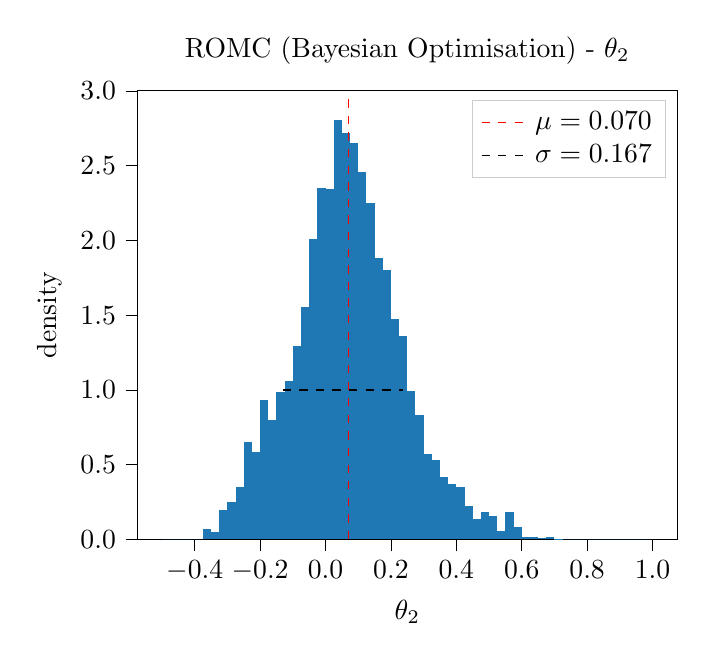
\begin{tikzpicture}

\definecolor{color0}{rgb}{0.12156862745098,0.466666666666667,0.705882352941177}

\begin{axis}[
legend cell align={left},
legend style={fill opacity=0.8, draw opacity=1, text opacity=1, draw=white!80!black},
tick align=outside,
tick pos=left,
title={ROMC (Bayesian Optimisation) - \(\displaystyle \theta_2\)},
x grid style={white!69.0196078431373!black},
xlabel={\(\displaystyle \theta_2\)},
xmin=-0.575, xmax=1.075,
xtick style={color=black},
xtick={-0.6,-0.4,-0.2,0,0.2,0.4,0.6,0.8,1,1.2},
xticklabels={
  \(\displaystyle {\ensuremath{-}0.6}\),
  \(\displaystyle {\ensuremath{-}0.4}\),
  \(\displaystyle {\ensuremath{-}0.2}\),
  \(\displaystyle {0.0}\),
  \(\displaystyle {0.2}\),
  \(\displaystyle {0.4}\),
  \(\displaystyle {0.6}\),
  \(\displaystyle {0.8}\),
  \(\displaystyle {1.0}\),
  \(\displaystyle {1.2}\)
},
y grid style={white!69.0196078431373!black},
ylabel={density},
ymin=0, ymax=3,
ytick style={color=black},
ytick={0,0.5,1,1.5,2,2.5,3},
yticklabels={
  \(\displaystyle {0.0}\),
  \(\displaystyle {0.5}\),
  \(\displaystyle {1.0}\),
  \(\displaystyle {1.5}\),
  \(\displaystyle {2.0}\),
  \(\displaystyle {2.5}\),
  \(\displaystyle {3.0}\)
}
]
\draw[draw=none,fill=color0] (axis cs:-0.5,0) rectangle (axis cs:-0.475,0);
\draw[draw=none,fill=color0] (axis cs:-0.475,0) rectangle (axis cs:-0.45,0);
\draw[draw=none,fill=color0] (axis cs:-0.45,0) rectangle (axis cs:-0.425,0);
\draw[draw=none,fill=color0] (axis cs:-0.425,0) rectangle (axis cs:-0.4,0);
\draw[draw=none,fill=color0] (axis cs:-0.4,0) rectangle (axis cs:-0.375,0);
\draw[draw=none,fill=color0] (axis cs:-0.375,0) rectangle (axis cs:-0.35,0.0710656818158832);
\draw[draw=none,fill=color0] (axis cs:-0.35,0) rectangle (axis cs:-0.325,0.0516473550957937);
\draw[draw=none,fill=color0] (axis cs:-0.325,0) rectangle (axis cs:-0.3,0.194048417709784);
\draw[draw=none,fill=color0] (axis cs:-0.3,0) rectangle (axis cs:-0.275,0.2505503544856);
\draw[draw=none,fill=color0] (axis cs:-0.275,0) rectangle (axis cs:-0.25,0.348585934523831);
\draw[draw=none,fill=color0] (axis cs:-0.25,0) rectangle (axis cs:-0.225,0.648086654282988);
\draw[draw=none,fill=color0] (axis cs:-0.225,0) rectangle (axis cs:-0.2,0.583763447022691);
\draw[draw=none,fill=color0] (axis cs:-0.2,0) rectangle (axis cs:-0.175,0.929922090706508);
\draw[draw=none,fill=color0] (axis cs:-0.175,0) rectangle (axis cs:-0.15,0.79776958941701);
\draw[draw=none,fill=color0] (axis cs:-0.15,0) rectangle (axis cs:-0.125,0.987907371884556);
\draw[draw=none,fill=color0] (axis cs:-0.125,0) rectangle (axis cs:-0.1,1.05978215064711);
\draw[draw=none,fill=color0] (axis cs:-0.1,0) rectangle (axis cs:-0.075,1.2930717702704);
\draw[draw=none,fill=color0] (axis cs:-0.075,0) rectangle (axis cs:-0.05,1.55481463251829);
\draw[draw=none,fill=color0] (axis cs:-0.05,0) rectangle (axis cs:-0.025,2.01101046094927);
\draw[draw=none,fill=color0] (axis cs:-0.025,0) rectangle (axis cs:0,2.35069632905971);
\draw[draw=none,fill=color0] (axis cs:0,0) rectangle (axis cs:0.025,2.34206596162857);
\draw[draw=none,fill=color0] (axis cs:0.025,0) rectangle (axis cs:0.05,2.80716185647295);
\draw[draw=none,fill=color0] (axis cs:0.05,0) rectangle (axis cs:0.0750000000000001,2.71681269742808);
\draw[draw=none,fill=color0] (axis cs:0.0750000000000001,0) rectangle (axis cs:0.1,2.65275918915001);
\draw[draw=none,fill=color0] (axis cs:0.1,0) rectangle (axis cs:0.125,2.45763197551135);
\draw[draw=none,fill=color0] (axis cs:0.125,0) rectangle (axis cs:0.15,2.24848041479702);
\draw[draw=none,fill=color0] (axis cs:0.15,0) rectangle (axis cs:0.175,1.8837125413398);
\draw[draw=none,fill=color0] (axis cs:0.175,0) rectangle (axis cs:0.2,1.80455589005721);
\draw[draw=none,fill=color0] (axis cs:0.2,0) rectangle (axis cs:0.225,1.47147764701123);
\draw[draw=none,fill=color0] (axis cs:0.225,0) rectangle (axis cs:0.25,1.35887832193294);
\draw[draw=none,fill=color0] (axis cs:0.25,0) rectangle (axis cs:0.275,0.990739211197902);
\draw[draw=none,fill=color0] (axis cs:0.275,0) rectangle (axis cs:0.3,0.834853199472739);
\draw[draw=none,fill=color0] (axis cs:0.3,0) rectangle (axis cs:0.325,0.568255755544842);
\draw[draw=none,fill=color0] (axis cs:0.325,0) rectangle (axis cs:0.35,0.531441844471339);
\draw[draw=none,fill=color0] (axis cs:0.35,0) rectangle (axis cs:0.375,0.415606131606362);
\draw[draw=none,fill=color0] (axis cs:0.375,0) rectangle (axis cs:0.4,0.366790615823915);
\draw[draw=none,fill=color0] (axis cs:0.4,0) rectangle (axis cs:0.425,0.350473827399395);
\draw[draw=none,fill=color0] (axis cs:0.425,0) rectangle (axis cs:0.45,0.220883466441019);
\draw[draw=none,fill=color0] (axis cs:0.45,0) rectangle (axis cs:0.475,0.136737383987297);
\draw[draw=none,fill=color0] (axis cs:0.475,0) rectangle (axis cs:0.5,0.185283200787522);
\draw[draw=none,fill=color0] (axis cs:0.5,0) rectangle (axis cs:0.525,0.154672366305157);
\draw[draw=none,fill=color0] (axis cs:0.525,0) rectangle (axis cs:0.55,0.0558276893202577);
\draw[draw=none,fill=color0] (axis cs:0.55,0) rectangle (axis cs:0.575,0.179619522160829);
\draw[draw=none,fill=color0] (axis cs:0.575,0) rectangle (axis cs:0.6,0.0788869523003634);
\draw[draw=none,fill=color0] (axis cs:0.6,0) rectangle (axis cs:0.625,0.0133500996200616);
\draw[draw=none,fill=color0] (axis cs:0.625,0) rectangle (axis cs:0.65,0.0134849491111732);
\draw[draw=none,fill=color0] (axis cs:0.65,0) rectangle (axis cs:0.675,0.00943946437782135);
\draw[draw=none,fill=color0] (axis cs:0.675,0) rectangle (axis cs:0.7,0.0140243470756202);
\draw[draw=none,fill=color0] (axis cs:0.7,0) rectangle (axis cs:0.725,0.00337123727779334);
\draw[draw=none,fill=color0] (axis cs:0.725,0) rectangle (axis cs:0.75,0);
\draw[draw=none,fill=color0] (axis cs:0.75,0) rectangle (axis cs:0.775,0);
\draw[draw=none,fill=color0] (axis cs:0.775,0) rectangle (axis cs:0.8,0);
\draw[draw=none,fill=color0] (axis cs:0.8,0) rectangle (axis cs:0.825,0);
\draw[draw=none,fill=color0] (axis cs:0.825,0) rectangle (axis cs:0.85,0);
\draw[draw=none,fill=color0] (axis cs:0.85,0) rectangle (axis cs:0.875,0);
\draw[draw=none,fill=color0] (axis cs:0.875,0) rectangle (axis cs:0.9,0);
\draw[draw=none,fill=color0] (axis cs:0.9,0) rectangle (axis cs:0.925,0);
\draw[draw=none,fill=color0] (axis cs:0.925,0) rectangle (axis cs:0.95,0);
\draw[draw=none,fill=color0] (axis cs:0.95,0) rectangle (axis cs:0.975,0);
\draw[draw=none,fill=color0] (axis cs:0.975,0) rectangle (axis cs:1,0);
\addplot [semithick, red, dashed]
table {%
0.070389896781954 0
0.070389896781954 3
};
\addlegendentry{$\mu = 0.070$}
\addplot [semithick, black, dashed]
table {%
-0.131187651225067 1
0.236045424145365 1
};
\addlegendentry{$\sigma = 0.167$}
\end{axis}

\end{tikzpicture}

    }
    \resizebox{.24\columnwidth}{!}{%
      % This file was created with tikzplotlib v0.9.12.
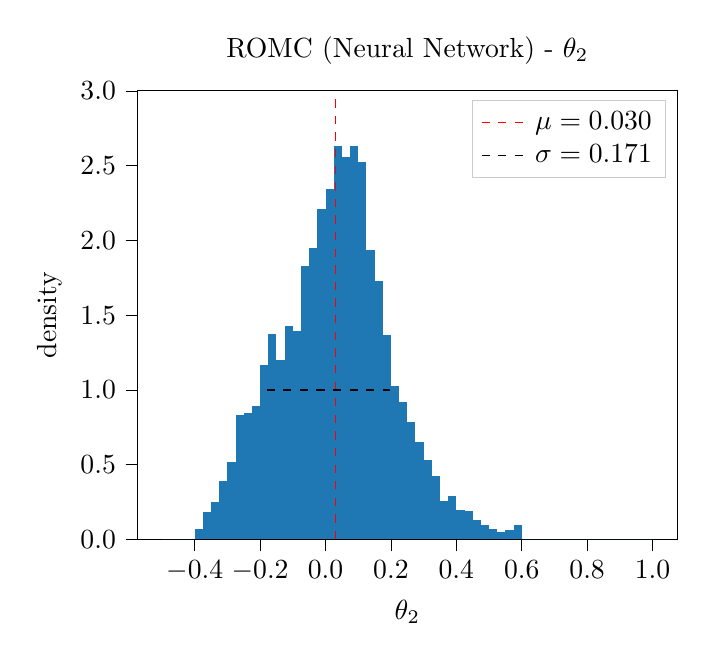
\begin{tikzpicture}

\definecolor{color0}{rgb}{0.12156862745098,0.466666666666667,0.705882352941177}

\begin{axis}[
legend cell align={left},
legend style={fill opacity=0.8, draw opacity=1, text opacity=1, draw=white!80!black},
tick align=outside,
tick pos=left,
title={ROMC (Neural Network) - \(\displaystyle \theta_2\)},
x grid style={white!69.0196078431373!black},
xlabel={\(\displaystyle \theta_2\)},
xmin=-0.575, xmax=1.075,
xtick style={color=black},
xtick={-0.6,-0.4,-0.2,0,0.2,0.4,0.6,0.8,1,1.2},
xticklabels={
  \(\displaystyle {\ensuremath{-}0.6}\),
  \(\displaystyle {\ensuremath{-}0.4}\),
  \(\displaystyle {\ensuremath{-}0.2}\),
  \(\displaystyle {0.0}\),
  \(\displaystyle {0.2}\),
  \(\displaystyle {0.4}\),
  \(\displaystyle {0.6}\),
  \(\displaystyle {0.8}\),
  \(\displaystyle {1.0}\),
  \(\displaystyle {1.2}\)
},
y grid style={white!69.0196078431373!black},
ylabel={density},
ymin=0, ymax=3,
ytick style={color=black},
ytick={0,0.5,1,1.5,2,2.5,3},
yticklabels={
  \(\displaystyle {0.0}\),
  \(\displaystyle {0.5}\),
  \(\displaystyle {1.0}\),
  \(\displaystyle {1.5}\),
  \(\displaystyle {2.0}\),
  \(\displaystyle {2.5}\),
  \(\displaystyle {3.0}\)
}
]
\draw[draw=none,fill=color0] (axis cs:-0.5,0) rectangle (axis cs:-0.475,0);
\draw[draw=none,fill=color0] (axis cs:-0.475,0) rectangle (axis cs:-0.45,0);
\draw[draw=none,fill=color0] (axis cs:-0.45,0) rectangle (axis cs:-0.425,0);
\draw[draw=none,fill=color0] (axis cs:-0.425,0) rectangle (axis cs:-0.4,0);
\draw[draw=none,fill=color0] (axis cs:-0.4,0) rectangle (axis cs:-0.375,0.0687105672242381);
\draw[draw=none,fill=color0] (axis cs:-0.375,0) rectangle (axis cs:-0.35,0.184372208227465);
\draw[draw=none,fill=color0] (axis cs:-0.35,0) rectangle (axis cs:-0.325,0.251601377874948);
\draw[draw=none,fill=color0] (axis cs:-0.325,0) rectangle (axis cs:-0.3,0.39271865402813);
\draw[draw=none,fill=color0] (axis cs:-0.3,0) rectangle (axis cs:-0.275,0.516086691042045);
\draw[draw=none,fill=color0] (axis cs:-0.275,0) rectangle (axis cs:-0.25,0.829805712987072);
\draw[draw=none,fill=color0] (axis cs:-0.25,0) rectangle (axis cs:-0.225,0.847041859829425);
\draw[draw=none,fill=color0] (axis cs:-0.225,0) rectangle (axis cs:-0.2,0.888673668222991);
\draw[draw=none,fill=color0] (axis cs:-0.2,0) rectangle (axis cs:-0.175,1.16327691119626);
\draw[draw=none,fill=color0] (axis cs:-0.175,0) rectangle (axis cs:-0.15,1.37486835291373);
\draw[draw=none,fill=color0] (axis cs:-0.15,0) rectangle (axis cs:-0.125,1.19991232691807);
\draw[draw=none,fill=color0] (axis cs:-0.125,0) rectangle (axis cs:-0.1,1.42636185782617);
\draw[draw=none,fill=color0] (axis cs:-0.1,0) rectangle (axis cs:-0.075,1.39151225358654);
\draw[draw=none,fill=color0] (axis cs:-0.075,0) rectangle (axis cs:-0.05,1.82926351678107);
\draw[draw=none,fill=color0] (axis cs:-0.05,0) rectangle (axis cs:-0.025,1.94594508515498);
\draw[draw=none,fill=color0] (axis cs:-0.025,0) rectangle (axis cs:0,2.2129470534662);
\draw[draw=none,fill=color0] (axis cs:0,0) rectangle (axis cs:0.025,2.34655785188779);
\draw[draw=none,fill=color0] (axis cs:0.025,0) rectangle (axis cs:0.05,2.63158719290653);
\draw[draw=none,fill=color0] (axis cs:0.05,0) rectangle (axis cs:0.0750000000000001,2.55685248411093);
\draw[draw=none,fill=color0] (axis cs:0.0750000000000001,0) rectangle (axis cs:0.1,2.63080691718184);
\draw[draw=none,fill=color0] (axis cs:0.1,0) rectangle (axis cs:0.125,2.52614922878044);
\draw[draw=none,fill=color0] (axis cs:0.125,0) rectangle (axis cs:0.15,1.93355077757299);
\draw[draw=none,fill=color0] (axis cs:0.15,0) rectangle (axis cs:0.175,1.72788273613444);
\draw[draw=none,fill=color0] (axis cs:0.175,0) rectangle (axis cs:0.2,1.36820910319437);
\draw[draw=none,fill=color0] (axis cs:0.2,0) rectangle (axis cs:0.225,1.0258751741395);
\draw[draw=none,fill=color0] (axis cs:0.225,0) rectangle (axis cs:0.25,0.915348210439271);
\draw[draw=none,fill=color0] (axis cs:0.25,0) rectangle (axis cs:0.275,0.784575688430834);
\draw[draw=none,fill=color0] (axis cs:0.275,0) rectangle (axis cs:0.3,0.649930571025344);
\draw[draw=none,fill=color0] (axis cs:0.3,0) rectangle (axis cs:0.325,0.528011081166735);
\draw[draw=none,fill=color0] (axis cs:0.325,0) rectangle (axis cs:0.35,0.423788895495386);
\draw[draw=none,fill=color0] (axis cs:0.35,0) rectangle (axis cs:0.375,0.255909163140911);
\draw[draw=none,fill=color0] (axis cs:0.375,0) rectangle (axis cs:0.4,0.28970067094874);
\draw[draw=none,fill=color0] (axis cs:0.4,0) rectangle (axis cs:0.425,0.19412252617457);
\draw[draw=none,fill=color0] (axis cs:0.425,0) rectangle (axis cs:0.45,0.189105171805318);
\draw[draw=none,fill=color0] (axis cs:0.45,0) rectangle (axis cs:0.475,0.127165545733375);
\draw[draw=none,fill=color0] (axis cs:0.475,0) rectangle (axis cs:0.5,0.0974061925124961);
\draw[draw=none,fill=color0] (axis cs:0.5,0) rectangle (axis cs:0.525,0.0718579504601718);
\draw[draw=none,fill=color0] (axis cs:0.525,0) rectangle (axis cs:0.55,0.0457277866564734);
\draw[draw=none,fill=color0] (axis cs:0.55,0) rectangle (axis cs:0.575,0.0587928685583229);
\draw[draw=none,fill=color0] (axis cs:0.575,0) rectangle (axis cs:0.6,0.0979881142638707);
\draw[draw=none,fill=color0] (axis cs:0.6,0) rectangle (axis cs:0.625,0);
\draw[draw=none,fill=color0] (axis cs:0.625,0) rectangle (axis cs:0.65,0);
\draw[draw=none,fill=color0] (axis cs:0.65,0) rectangle (axis cs:0.675,0);
\draw[draw=none,fill=color0] (axis cs:0.675,0) rectangle (axis cs:0.7,0);
\draw[draw=none,fill=color0] (axis cs:0.7,0) rectangle (axis cs:0.725,0);
\draw[draw=none,fill=color0] (axis cs:0.725,0) rectangle (axis cs:0.75,0);
\draw[draw=none,fill=color0] (axis cs:0.75,0) rectangle (axis cs:0.775,0);
\draw[draw=none,fill=color0] (axis cs:0.775,0) rectangle (axis cs:0.8,0);
\draw[draw=none,fill=color0] (axis cs:0.8,0) rectangle (axis cs:0.825,0);
\draw[draw=none,fill=color0] (axis cs:0.825,0) rectangle (axis cs:0.85,0);
\draw[draw=none,fill=color0] (axis cs:0.85,0) rectangle (axis cs:0.875,0);
\draw[draw=none,fill=color0] (axis cs:0.875,0) rectangle (axis cs:0.9,0);
\draw[draw=none,fill=color0] (axis cs:0.9,0) rectangle (axis cs:0.925,0);
\draw[draw=none,fill=color0] (axis cs:0.925,0) rectangle (axis cs:0.95,0);
\draw[draw=none,fill=color0] (axis cs:0.95,0) rectangle (axis cs:0.975,0);
\draw[draw=none,fill=color0] (axis cs:0.975,0) rectangle (axis cs:1,0);
\addplot [semithick, red, dashed]
table {%
0.0301562808023854 0
0.0301562808023854 3
};
\addlegendentry{$\mu = 0.030$}
\addplot [semithick, black, dashed]
table {%
-0.180267449762181 1
0.196611267527429 1
};
\addlegendentry{$\sigma = 0.171$}
\end{axis}

\end{tikzpicture}

    }
    \end{center}
    \caption[MA2 example, evaluation of the marginal
    distributions.]{Histogram of the marginal posterior distributions
      using three different inference approaches; (a) in the first
      row, the samples are obtained using Rejection ABC sampling (b)
      in the second row, using ROMC with a gradient-based optimiser
      and (c) in the third row, using ROMC with Bayesian optimisation
      approach. The vertical (red) line represents the samples mean
      \(\mu\) and the horizontal (black) the standard deviation
      \(\sigma\).}
  \label{fig:ma2_3}
\end{figure}

\begin{figure}[ht]
  \begin{center}
    \resizebox{.32\columnwidth}{!}{%
      % This file was created with tikzplotlib v0.9.12.
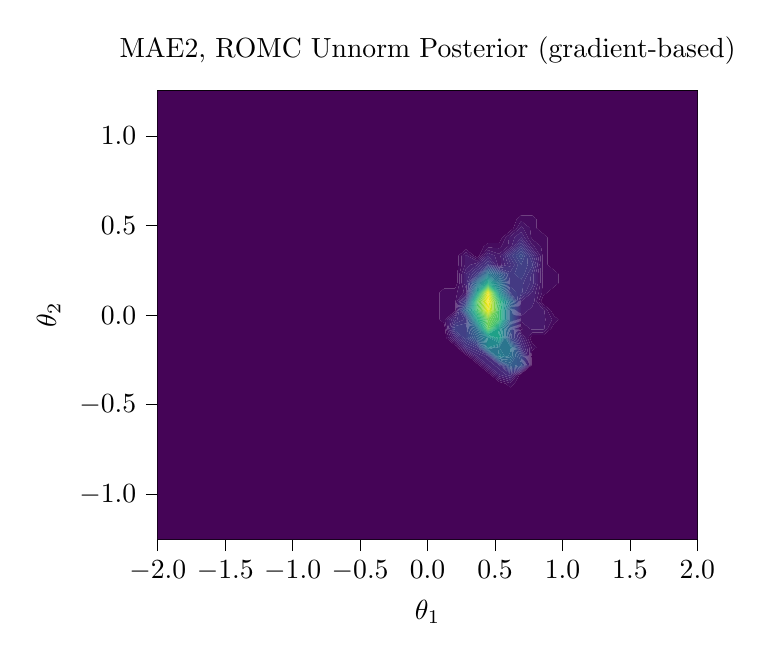
\begin{tikzpicture}

\definecolor{color0}{rgb}{0.269944,0.014625,0.341379}
\definecolor{color1}{rgb}{0.276022,0.044167,0.370164}
\definecolor{color2}{rgb}{0.280267,0.073417,0.397163}
\definecolor{color3}{rgb}{0.282656,0.100196,0.42216}
\definecolor{color4}{rgb}{0.283072,0.130895,0.449241}
\definecolor{color5}{rgb}{0.281412,0.155834,0.469201}
\definecolor{color6}{rgb}{0.278012,0.180367,0.486697}
\definecolor{color7}{rgb}{0.273006,0.20452,0.501721}
\definecolor{color8}{rgb}{0.26658,0.228262,0.514349}
\definecolor{color9}{rgb}{0.258965,0.251537,0.524736}
\definecolor{color10}{rgb}{0.250425,0.27429,0.533103}
\definecolor{color11}{rgb}{0.241237,0.296485,0.539709}
\definecolor{color12}{rgb}{0.229739,0.322361,0.545706}
\definecolor{color13}{rgb}{0.220057,0.343307,0.549413}
\definecolor{color14}{rgb}{0.210503,0.363727,0.552206}
\definecolor{color15}{rgb}{0.201239,0.38367,0.554294}
\definecolor{color16}{rgb}{0.192357,0.403199,0.555836}
\definecolor{color17}{rgb}{0.183898,0.422383,0.556944}
\definecolor{color18}{rgb}{0.175841,0.44129,0.557685}
\definecolor{color19}{rgb}{0.168126,0.459988,0.558082}
\definecolor{color20}{rgb}{0.160665,0.47854,0.558115}
\definecolor{color21}{rgb}{0.151918,0.500685,0.557587}
\definecolor{color22}{rgb}{0.144759,0.519093,0.556572}
\definecolor{color23}{rgb}{0.13777,0.537492,0.554906}
\definecolor{color24}{rgb}{0.131172,0.555899,0.552459}
\definecolor{color25}{rgb}{0.125394,0.574318,0.549086}
\definecolor{color26}{rgb}{0.121148,0.592739,0.544641}
\definecolor{color27}{rgb}{0.119423,0.611141,0.538982}
\definecolor{color28}{rgb}{0.12138,0.629492,0.531973}
\definecolor{color29}{rgb}{0.130067,0.651384,0.521608}
\definecolor{color30}{rgb}{0.143303,0.669459,0.511215}
\definecolor{color31}{rgb}{0.162016,0.687316,0.499129}
\definecolor{color32}{rgb}{0.185783,0.704891,0.485273}
\definecolor{color33}{rgb}{0.214,0.722114,0.469588}
\definecolor{color34}{rgb}{0.24607,0.73891,0.452024}
\definecolor{color35}{rgb}{0.281477,0.755203,0.432552}
\definecolor{color36}{rgb}{0.319809,0.770914,0.411152}
\definecolor{color37}{rgb}{0.369214,0.788888,0.382914}
\definecolor{color38}{rgb}{0.412913,0.803041,0.357269}
\definecolor{color39}{rgb}{0.458674,0.816363,0.329727}
\definecolor{color40}{rgb}{0.506271,0.828786,0.300362}
\definecolor{color41}{rgb}{0.555484,0.840254,0.269281}
\definecolor{color42}{rgb}{0.606045,0.850733,0.236712}
\definecolor{color43}{rgb}{0.657642,0.860219,0.203082}
\definecolor{color44}{rgb}{0.709898,0.868751,0.169257}
\definecolor{color45}{rgb}{0.762373,0.876424,0.137064}
\definecolor{color46}{rgb}{0.82494,0.88472,0.106217}
\definecolor{color47}{rgb}{0.876168,0.891125,0.09525}
\definecolor{color48}{rgb}{0.926106,0.89733,0.104071}
\definecolor{color49}{rgb}{0.974417,0.90359,0.130215}

\begin{axis}[
tick align=outside,
tick pos=left,
title={MAE2, ROMC Unnorm Posterior (gradient-based)},
x grid style={white!69.0196078431373!black},
xlabel={\(\displaystyle \theta_1\)},
xmin=-2, xmax=2,
xtick style={color=black},
xtick={-2,-1.5,-1,-0.5,0,0.5,1,1.5,2},
xticklabels={
  \(\displaystyle {\ensuremath{-}2.0}\),
  \(\displaystyle {\ensuremath{-}1.5}\),
  \(\displaystyle {\ensuremath{-}1.0}\),
  \(\displaystyle {\ensuremath{-}0.5}\),
  \(\displaystyle {0.0}\),
  \(\displaystyle {0.5}\),
  \(\displaystyle {1.0}\),
  \(\displaystyle {1.5}\),
  \(\displaystyle {2.0}\)
},
y grid style={white!69.0196078431373!black},
ylabel={\(\displaystyle \theta_2\)},
ymin=-1.25, ymax=1.25,
ytick style={color=black},
ytick={-1.5,-1,-0.5,0,0.5,1,1.5},
yticklabels={
  \(\displaystyle {\ensuremath{-}1.5}\),
  \(\displaystyle {\ensuremath{-}1.0}\),
  \(\displaystyle {\ensuremath{-}0.5}\),
  \(\displaystyle {0.0}\),
  \(\displaystyle {0.5}\),
  \(\displaystyle {1.0}\),
  \(\displaystyle {1.5}\)
}
]
\addplot [draw=none, fill=color0]
table{%
x  y
-1.91836734693878 -1.25
-1.83673469387755 -1.25
-1.75510204081633 -1.25
-1.6734693877551 -1.25
-1.59183673469388 -1.25
-1.51020408163265 -1.25
-1.42857142857143 -1.25
-1.3469387755102 -1.25
-1.26530612244898 -1.25
-1.18367346938776 -1.25
-1.10204081632653 -1.25
-1.02040816326531 -1.25
-0.938775510204082 -1.25
-0.857142857142857 -1.25
-0.775510204081633 -1.25
-0.693877551020408 -1.25
-0.612244897959184 -1.25
-0.530612244897959 -1.25
-0.448979591836735 -1.25
-0.36734693877551 -1.25
-0.285714285714286 -1.25
-0.204081632653061 -1.25
-0.122448979591837 -1.25
-0.0408163265306123 -1.25
0.0408163265306123 -1.25
0.122448979591836 -1.25
0.204081632653061 -1.25
0.285714285714286 -1.25
0.36734693877551 -1.25
0.448979591836734 -1.25
0.530612244897959 -1.25
0.612244897959183 -1.25
0.693877551020408 -1.25
0.775510204081633 -1.25
0.857142857142857 -1.25
0.938775510204081 -1.25
1.02040816326531 -1.25
1.10204081632653 -1.25
1.18367346938775 -1.25
1.26530612244898 -1.25
1.3469387755102 -1.25
1.42857142857143 -1.25
1.51020408163265 -1.25
1.59183673469388 -1.25
1.6734693877551 -1.25
1.75510204081633 -1.25
1.83673469387755 -1.25
1.91836734693878 -1.25
2 -1.25
2 -1.19897959183673
2 -1.14795918367347
2 -1.0969387755102
2 -1.04591836734694
2 -0.994897959183674
2 -0.943877551020408
2 -0.892857142857143
2 -0.841836734693878
2 -0.790816326530612
2 -0.739795918367347
2 -0.688775510204082
2 -0.637755102040816
2 -0.586734693877551
2 -0.535714285714286
2 -0.48469387755102
2 -0.433673469387755
2 -0.38265306122449
2 -0.331632653061224
2 -0.280612244897959
2 -0.229591836734694
2 -0.178571428571429
2 -0.127551020408163
2 -0.0765306122448979
2 -0.0255102040816326
2 0.0255102040816326
2 0.0765306122448979
2 0.127551020408163
2 0.178571428571429
2 0.229591836734694
2 0.280612244897959
2 0.331632653061225
2 0.38265306122449
2 0.433673469387755
2 0.48469387755102
2 0.535714285714286
2 0.586734693877551
2 0.637755102040816
2 0.688775510204082
2 0.739795918367347
2 0.790816326530612
2 0.841836734693878
2 0.892857142857143
2 0.943877551020408
2 0.994897959183674
2 1.04591836734694
2 1.0969387755102
2 1.14795918367347
2 1.19897959183673
2 1.25
1.91836734693878 1.25
1.83673469387755 1.25
1.75510204081633 1.25
1.6734693877551 1.25
1.59183673469388 1.25
1.51020408163265 1.25
1.42857142857143 1.25
1.3469387755102 1.25
1.26530612244898 1.25
1.18367346938775 1.25
1.10204081632653 1.25
1.02040816326531 1.25
0.938775510204081 1.25
0.857142857142857 1.25
0.775510204081633 1.25
0.693877551020408 1.25
0.612244897959183 1.25
0.530612244897959 1.25
0.448979591836734 1.25
0.36734693877551 1.25
0.285714285714286 1.25
0.204081632653061 1.25
0.122448979591836 1.25
0.0408163265306123 1.25
-0.0408163265306123 1.25
-0.122448979591837 1.25
-0.204081632653061 1.25
-0.285714285714286 1.25
-0.36734693877551 1.25
-0.448979591836735 1.25
-0.530612244897959 1.25
-0.612244897959184 1.25
-0.693877551020408 1.25
-0.775510204081633 1.25
-0.857142857142857 1.25
-0.938775510204082 1.25
-1.02040816326531 1.25
-1.10204081632653 1.25
-1.18367346938776 1.25
-1.26530612244898 1.25
-1.3469387755102 1.25
-1.42857142857143 1.25
-1.51020408163265 1.25
-1.59183673469388 1.25
-1.6734693877551 1.25
-1.75510204081633 1.25
-1.83673469387755 1.25
-1.91836734693878 1.25
-2 1.25
-2 1.19897959183673
-2 1.14795918367347
-2 1.0969387755102
-2 1.04591836734694
-2 0.994897959183674
-2 0.943877551020408
-2 0.892857142857143
-2 0.841836734693878
-2 0.790816326530612
-2 0.739795918367347
-2 0.688775510204082
-2 0.637755102040816
-2 0.586734693877551
-2 0.535714285714286
-2 0.48469387755102
-2 0.433673469387755
-2 0.38265306122449
-2 0.331632653061225
-2 0.280612244897959
-2 0.229591836734694
-2 0.178571428571429
-2 0.127551020408163
-2 0.0765306122448979
-2 0.0255102040816326
-2 -0.0255102040816326
-2 -0.0765306122448979
-2 -0.127551020408163
-2 -0.178571428571429
-2 -0.229591836734694
-2 -0.280612244897959
-2 -0.331632653061224
-2 -0.38265306122449
-2 -0.433673469387755
-2 -0.48469387755102
-2 -0.535714285714286
-2 -0.586734693877551
-2 -0.637755102040816
-2 -0.688775510204082
-2 -0.739795918367347
-2 -0.790816326530612
-2 -0.841836734693878
-2 -0.892857142857143
-2 -0.943877551020408
-2 -0.994897959183674
-2 -1.04591836734694
-2 -1.0969387755102
-2 -1.14795918367347
-2 -1.19897959183673
-2 -1.25
-1.91836734693878 -1.25

0.579591836734694 -0.38265306122449
0.530612244897959 -0.372448979591837
0.465306122448979 -0.331632653061224
0.448979591836734 -0.321428571428571
0.383673469387755 -0.280612244897959
0.36734693877551 -0.270408163265306
0.302040816326531 -0.229591836734694
0.285714285714286 -0.221938775510204
0.216326530612245 -0.178571428571429
0.204081632653061 -0.168367346938776
0.138775510204081 -0.127551020408163
0.130612244897959 -0.0765306122448979
0.122448979591836 -0.0459183673469387
0.0897959183673468 -0.0255102040816326
0.0897959183673468 0.0255102040816326
0.0897959183673468 0.0765306122448979
0.0897959183673468 0.127551020408163
0.122448979591836 0.147959183673469
0.204081632653061 0.147959183673469
0.220408163265306 0.178571428571429
0.220408163265306 0.229591836734694
0.228571428571428 0.280612244897959
0.228571428571428 0.331632653061225
0.285714285714286 0.36734693877551
0.342857142857143 0.331632653061225
0.36734693877551 0.321428571428572
0.383673469387755 0.331632653061225
0.416326530612245 0.38265306122449
0.448979591836734 0.403061224489796
0.530612244897959 0.403061224489796
0.555102040816326 0.433673469387755
0.612244897959183 0.469387755102041
0.636734693877551 0.48469387755102
0.661224489795918 0.535714285714286
0.693877551020408 0.556122448979592
0.775510204081633 0.556122448979592
0.808163265306122 0.535714285714286
0.808163265306122 0.48469387755102
0.857142857142857 0.454081632653061
0.889795918367347 0.433673469387755
0.889795918367347 0.38265306122449
0.889795918367347 0.331632653061225
0.889795918367347 0.280612244897959
0.938775510204081 0.25
0.971428571428571 0.229591836734694
0.971428571428571 0.178571428571429
0.938775510204081 0.158163265306123
0.889795918367347 0.127551020408163
0.857142857142857 0.107142857142857
0.840816326530612 0.0765306122448979
0.857142857142857 0.0612244897959183
0.914285714285714 0.0255102040816326
0.938775510204081 -0.00510204081632653
0.971428571428571 -0.0255102040816326
0.938775510204081 -0.0459183673469387
0.914285714285714 -0.0765306122448979
0.857142857142857 -0.112244897959184
0.775510204081633 -0.112244897959184
0.759183673469388 -0.127551020408163
0.775510204081633 -0.158163265306122
0.808163265306122 -0.178571428571429
0.775510204081633 -0.198979591836735
0.768513119533528 -0.229591836734694
0.769387755102041 -0.280612244897959
0.693877551020408 -0.32780612244898
0.681632653061224 -0.331632653061224
0.644897959183673 -0.38265306122449
0.612244897959183 -0.403061224489796
0.579591836734694 -0.38265306122449
};
\addplot [draw=none, fill=color1]
table{%
x  y
0.612244897959183 -0.403061224489796
0.644897959183673 -0.38265306122449
0.681632653061224 -0.331632653061224
0.693877551020408 -0.32780612244898
0.769387755102041 -0.280612244897959
0.768513119533528 -0.229591836734694
0.775510204081633 -0.198979591836735
0.808163265306122 -0.178571428571429
0.775510204081633 -0.158163265306122
0.759183673469388 -0.127551020408163
0.775510204081633 -0.112244897959184
0.857142857142857 -0.112244897959184
0.914285714285714 -0.0765306122448979
0.938775510204081 -0.0459183673469387
0.971428571428571 -0.0255102040816326
0.938775510204081 -0.00510204081632653
0.914285714285714 0.0255102040816326
0.857142857142857 0.0612244897959183
0.840816326530612 0.0765306122448979
0.857142857142857 0.107142857142857
0.889795918367347 0.127551020408163
0.938775510204081 0.158163265306123
0.971428571428571 0.178571428571429
0.971428571428571 0.229591836734694
0.938775510204081 0.25
0.889795918367347 0.280612244897959
0.889795918367347 0.331632653061225
0.889795918367347 0.38265306122449
0.889795918367347 0.433673469387755
0.857142857142857 0.454081632653061
0.808163265306122 0.48469387755102
0.808163265306122 0.535714285714286
0.775510204081633 0.556122448979592
0.693877551020408 0.556122448979592
0.661224489795918 0.535714285714286
0.636734693877551 0.48469387755102
0.612244897959183 0.469387755102041
0.555102040816326 0.433673469387755
0.530612244897959 0.403061224489796
0.448979591836734 0.403061224489796
0.416326530612245 0.38265306122449
0.383673469387755 0.331632653061225
0.36734693877551 0.321428571428572
0.342857142857143 0.331632653061225
0.285714285714286 0.36734693877551
0.228571428571428 0.331632653061225
0.228571428571428 0.280612244897959
0.220408163265306 0.229591836734694
0.220408163265306 0.178571428571429
0.204081632653061 0.147959183673469
0.122448979591836 0.147959183673469
0.0897959183673468 0.127551020408163
0.0897959183673468 0.0765306122448979
0.0897959183673468 0.0255102040816326
0.0897959183673468 -0.0255102040816326
0.122448979591836 -0.0459183673469387
0.130612244897959 -0.0765306122448979
0.138775510204081 -0.127551020408163
0.204081632653061 -0.168367346938776
0.216326530612245 -0.178571428571429
0.285714285714286 -0.221938775510204
0.302040816326531 -0.229591836734694
0.36734693877551 -0.270408163265306
0.383673469387755 -0.280612244897959
0.448979591836734 -0.321428571428571
0.465306122448979 -0.331632653061224
0.530612244897959 -0.372448979591837
0.579591836734694 -0.38265306122449
0.612244897959183 -0.403061224489796

0.481632653061224 -0.331632653061224
0.448979591836734 -0.311224489795918
0.4 -0.280612244897959
0.36734693877551 -0.260204081632653
0.318367346938775 -0.229591836734694
0.285714285714286 -0.214285714285714
0.228571428571428 -0.178571428571429
0.204081632653061 -0.158163265306122
0.155102040816326 -0.127551020408163
0.138775510204081 -0.0765306122448979
0.127891156462585 -0.0255102040816326
0.204081632653061 0.0221088435374149
0.205895691609977 0.0255102040816326
0.20734693877551 0.0765306122448979
0.220408163265306 0.127551020408163
0.236734693877551 0.178571428571429
0.236734693877551 0.229591836734694
0.253061224489796 0.280612244897959
0.253061224489796 0.331632653061225
0.285714285714286 0.352040816326531
0.318367346938775 0.331632653061225
0.36734693877551 0.311224489795918
0.4 0.331632653061225
0.448979591836734 0.377551020408163
0.530612244897959 0.372448979591837
0.546938775510204 0.38265306122449
0.579591836734694 0.433673469387755
0.612244897959183 0.454081632653061
0.661224489795918 0.48469387755102
0.693877551020408 0.525510204081633
0.759183673469388 0.48469387755102
0.76734693877551 0.433673469387755
0.775510204081633 0.423469387755102
0.840816326530612 0.38265306122449
0.851700680272108 0.331632653061225
0.853061224489795 0.280612244897959
0.851700680272108 0.229591836734694
0.851700680272108 0.178571428571429
0.848979591836734 0.127551020408163
0.824489795918367 0.0765306122448979
0.857142857142857 0.0459183673469387
0.889795918367347 0.0255102040816326
0.922448979591836 -0.0255102040816326
0.889795918367347 -0.0765306122448979
0.857142857142857 -0.096938775510204
0.775510204081633 -0.096938775510204
0.742857142857143 -0.127551020408163
0.770068027210884 -0.178571428571429
0.761516034985423 -0.229591836734694
0.763265306122449 -0.280612244897959
0.693877551020408 -0.323979591836735
0.669387755102041 -0.331632653061224
0.612244897959183 -0.379251700680272
0.530612244897959 -0.362244897959184
0.481632653061224 -0.331632653061224
};
\addplot [draw=none, fill=color1]
table{%
x  y
0.693877551020408 -0.0816326530612244
0.710204081632653 -0.0765306122448979
0.693877551020408 -0.0663265306122448
0.691545189504373 -0.0765306122448979
0.693877551020408 -0.0816326530612244
};
\addplot [draw=none, fill=color2]
table{%
x  y
0.530612244897959 -0.362244897959184
0.612244897959183 -0.379251700680272
0.669387755102041 -0.331632653061224
0.693877551020408 -0.323979591836735
0.763265306122449 -0.280612244897959
0.761516034985423 -0.229591836734694
0.770068027210884 -0.178571428571429
0.742857142857143 -0.127551020408163
0.775510204081633 -0.096938775510204
0.857142857142857 -0.096938775510204
0.889795918367347 -0.0765306122448979
0.922448979591836 -0.0255102040816326
0.889795918367347 0.0255102040816326
0.857142857142857 0.0459183673469387
0.824489795918367 0.0765306122448979
0.848979591836734 0.127551020408163
0.851700680272109 0.178571428571429
0.851700680272109 0.229591836734694
0.853061224489795 0.280612244897959
0.851700680272109 0.331632653061225
0.840816326530612 0.38265306122449
0.775510204081633 0.423469387755102
0.76734693877551 0.433673469387755
0.759183673469388 0.48469387755102
0.693877551020408 0.525510204081633
0.661224489795918 0.48469387755102
0.612244897959183 0.454081632653061
0.579591836734694 0.433673469387755
0.546938775510204 0.38265306122449
0.530612244897959 0.372448979591837
0.448979591836734 0.377551020408163
0.4 0.331632653061225
0.36734693877551 0.311224489795918
0.318367346938775 0.331632653061225
0.285714285714286 0.352040816326531
0.253061224489796 0.331632653061225
0.253061224489796 0.280612244897959
0.236734693877551 0.229591836734694
0.236734693877551 0.178571428571429
0.220408163265306 0.127551020408163
0.20734693877551 0.0765306122448979
0.205895691609977 0.0255102040816326
0.204081632653061 0.0221088435374149
0.127891156462585 -0.0255102040816326
0.138775510204081 -0.0765306122448979
0.155102040816326 -0.127551020408163
0.204081632653061 -0.158163265306122
0.228571428571428 -0.178571428571429
0.285714285714286 -0.214285714285714
0.318367346938775 -0.229591836734694
0.36734693877551 -0.260204081632653
0.4 -0.280612244897959
0.448979591836734 -0.311224489795918
0.481632653061224 -0.331632653061224
0.530612244897959 -0.362244897959184

0.497959183673469 -0.331632653061224
0.448979591836734 -0.301020408163265
0.416326530612245 -0.280612244897959
0.36734693877551 -0.25
0.33469387755102 -0.229591836734694
0.285714285714286 -0.206632653061224
0.240816326530612 -0.178571428571429
0.204081632653061 -0.147959183673469
0.171428571428571 -0.127551020408163
0.146938775510204 -0.0765306122448979
0.14421768707483 -0.0255102040816326
0.204081632653061 0.0119047619047619
0.211337868480725 0.0255102040816326
0.217142857142857 0.0765306122448979
0.269387755102041 0.127551020408163
0.253061224489796 0.178571428571429
0.253061224489796 0.229591836734694
0.277551020408163 0.280612244897959
0.277551020408163 0.331632653061225
0.285714285714286 0.336734693877551
0.293877551020408 0.331632653061225
0.36734693877551 0.301020408163265
0.416326530612245 0.331632653061225
0.448979591836734 0.362244897959184
0.530612244897959 0.341836734693878
0.595918367346939 0.38265306122449
0.604081632653061 0.433673469387755
0.612244897959183 0.438775510204082
0.685714285714285 0.48469387755102
0.693877551020408 0.494897959183673
0.710204081632653 0.48469387755102
0.742857142857143 0.433673469387755
0.775510204081633 0.392857142857143
0.791836734693877 0.38265306122449
0.835374149659864 0.331632653061225
0.840816326530612 0.280612244897959
0.835374149659864 0.229591836734694
0.835374149659864 0.178571428571429
0.824489795918367 0.127551020408163
0.808163265306122 0.0765306122448979
0.857142857142857 0.0306122448979591
0.865306122448979 0.0255102040816326
0.873469387755102 -0.0255102040816326
0.865306122448979 -0.0765306122448979
0.857142857142857 -0.0816326530612244
0.775510204081633 -0.0816326530612244
0.759183673469388 -0.0765306122448979
0.693877551020408 -0.0357142857142857
0.684548104956268 -0.0765306122448979
0.693877551020408 -0.096938775510204
0.726530612244898 -0.127551020408163
0.753741496598639 -0.178571428571429
0.754518950437318 -0.229591836734694
0.757142857142857 -0.280612244897959
0.693877551020408 -0.32015306122449
0.657142857142857 -0.331632653061224
0.612244897959183 -0.369047619047619
0.530612244897959 -0.352040816326531
0.497959183673469 -0.331632653061224

0.691545189504373 -0.0765306122448979
0.693877551020408 -0.0663265306122448
0.710204081632653 -0.0765306122448979
0.693877551020408 -0.0816326530612244
0.691545189504373 -0.0765306122448979
};
\addplot [draw=none, fill=color3]
table{%
x  y
0.530612244897959 -0.352040816326531
0.612244897959183 -0.369047619047619
0.657142857142857 -0.331632653061224
0.693877551020408 -0.32015306122449
0.757142857142857 -0.280612244897959
0.754518950437318 -0.229591836734694
0.753741496598639 -0.178571428571429
0.726530612244898 -0.127551020408163
0.693877551020408 -0.096938775510204
0.684548104956268 -0.0765306122448979
0.693877551020408 -0.0357142857142857
0.759183673469388 -0.0765306122448979
0.775510204081633 -0.0816326530612244
0.857142857142857 -0.0816326530612244
0.865306122448979 -0.0765306122448979
0.873469387755102 -0.0255102040816326
0.865306122448979 0.0255102040816326
0.857142857142857 0.0306122448979591
0.808163265306122 0.0765306122448979
0.824489795918367 0.127551020408163
0.835374149659864 0.178571428571429
0.835374149659864 0.229591836734694
0.840816326530612 0.280612244897959
0.835374149659864 0.331632653061225
0.791836734693877 0.38265306122449
0.775510204081633 0.392857142857143
0.742857142857143 0.433673469387755
0.710204081632653 0.48469387755102
0.693877551020408 0.494897959183673
0.685714285714285 0.48469387755102
0.612244897959183 0.438775510204082
0.604081632653061 0.433673469387755
0.595918367346939 0.38265306122449
0.530612244897959 0.341836734693878
0.448979591836734 0.362244897959184
0.416326530612245 0.331632653061225
0.36734693877551 0.301020408163265
0.293877551020408 0.331632653061225
0.285714285714286 0.336734693877551
0.277551020408163 0.331632653061225
0.277551020408163 0.280612244897959
0.253061224489796 0.229591836734694
0.253061224489796 0.178571428571429
0.269387755102041 0.127551020408163
0.217142857142857 0.0765306122448979
0.211337868480725 0.0255102040816326
0.204081632653061 0.0119047619047619
0.14421768707483 -0.0255102040816326
0.146938775510204 -0.0765306122448979
0.171428571428571 -0.127551020408163
0.204081632653061 -0.147959183673469
0.240816326530612 -0.178571428571429
0.285714285714286 -0.206632653061224
0.33469387755102 -0.229591836734694
0.36734693877551 -0.25
0.416326530612245 -0.280612244897959
0.448979591836734 -0.301020408163265
0.497959183673469 -0.331632653061224
0.530612244897959 -0.352040816326531

0.514285714285714 -0.331632653061224
0.448979591836734 -0.290816326530612
0.432653061224489 -0.280612244897959
0.36734693877551 -0.239795918367347
0.351020408163265 -0.229591836734694
0.285714285714286 -0.198979591836735
0.253061224489796 -0.178571428571429
0.204081632653061 -0.137755102040816
0.187755102040816 -0.127551020408163
0.155102040816326 -0.0765306122448979
0.160544217687075 -0.0255102040816326
0.204081632653061 0.00170068027210884
0.216780045351474 0.0255102040816326
0.226938775510204 0.0765306122448979
0.285714285714286 0.122448979591837
0.288046647230321 0.127551020408163
0.285714285714286 0.147959183673469
0.269387755102041 0.178571428571429
0.269387755102041 0.229591836734694
0.285714285714286 0.260204081632653
0.318367346938775 0.280612244897959
0.36734693877551 0.290816326530612
0.432653061224489 0.331632653061225
0.448979591836734 0.346938775510204
0.497959183673469 0.331632653061225
0.519727891156462 0.280612244897959
0.530612244897959 0.277696793002916
0.546938775510204 0.280612244897959
0.541496598639456 0.331632653061225
0.612244897959183 0.375850340136054
0.62312925170068 0.38265306122449
0.644897959183673 0.433673469387755
0.693877551020408 0.464285714285714
0.718367346938775 0.433673469387755
0.764625850340136 0.38265306122449
0.775510204081633 0.372448979591837
0.819047619047619 0.331632653061225
0.828571428571428 0.280612244897959
0.819047619047619 0.229591836734694
0.819047619047619 0.178571428571429
0.8 0.127551020408163
0.791836734693877 0.0765306122448979
0.775510204081633 0.0459183673469387
0.742857142857143 0.0255102040816326
0.693877551020408 -0.00510204081632651
0.689212827988338 -0.0255102040816326
0.677551020408163 -0.0765306122448979
0.693877551020408 -0.112244897959184
0.710204081632653 -0.127551020408163
0.737414965986394 -0.178571428571429
0.747521865889213 -0.229591836734694
0.751020408163265 -0.280612244897959
0.693877551020408 -0.316326530612245
0.644897959183673 -0.331632653061224
0.612244897959183 -0.358843537414966
0.530612244897959 -0.341836734693878
0.514285714285714 -0.331632653061224
};
\addplot [draw=none, fill=color4]
table{%
x  y
0.530612244897959 -0.341836734693878
0.612244897959183 -0.358843537414966
0.644897959183673 -0.331632653061224
0.693877551020408 -0.316326530612245
0.751020408163265 -0.280612244897959
0.747521865889213 -0.229591836734694
0.737414965986394 -0.178571428571429
0.710204081632653 -0.127551020408163
0.693877551020408 -0.112244897959184
0.677551020408163 -0.0765306122448979
0.689212827988338 -0.0255102040816326
0.693877551020408 -0.00510204081632651
0.742857142857143 0.0255102040816326
0.775510204081633 0.0459183673469387
0.791836734693877 0.0765306122448979
0.8 0.127551020408163
0.819047619047619 0.178571428571429
0.819047619047619 0.229591836734694
0.828571428571428 0.280612244897959
0.819047619047619 0.331632653061225
0.775510204081633 0.372448979591837
0.764625850340136 0.38265306122449
0.718367346938775 0.433673469387755
0.693877551020408 0.464285714285714
0.644897959183673 0.433673469387755
0.62312925170068 0.38265306122449
0.612244897959183 0.375850340136054
0.541496598639456 0.331632653061225
0.546938775510204 0.280612244897959
0.530612244897959 0.277696793002916
0.519727891156462 0.280612244897959
0.497959183673469 0.331632653061225
0.448979591836734 0.346938775510204
0.43265306122449 0.331632653061225
0.36734693877551 0.290816326530612
0.318367346938775 0.280612244897959
0.285714285714286 0.260204081632653
0.269387755102041 0.229591836734694
0.269387755102041 0.178571428571429
0.285714285714286 0.147959183673469
0.288046647230321 0.127551020408163
0.285714285714286 0.122448979591837
0.226938775510204 0.0765306122448979
0.216780045351474 0.0255102040816326
0.204081632653061 0.00170068027210884
0.160544217687075 -0.0255102040816326
0.155102040816326 -0.0765306122448979
0.187755102040816 -0.127551020408163
0.204081632653061 -0.137755102040816
0.253061224489796 -0.178571428571429
0.285714285714286 -0.198979591836735
0.351020408163265 -0.229591836734694
0.36734693877551 -0.239795918367347
0.43265306122449 -0.280612244897959
0.448979591836734 -0.290816326530612
0.514285714285714 -0.331632653061224
0.530612244897959 -0.341836734693878

0.530612244897959 -0.331632653061224
0.530612244897959 -0.331632653061224
0.448979591836734 -0.280612244897959
0.448979591836734 -0.280612244897959
0.36734693877551 -0.229591836734694
0.36734693877551 -0.229591836734694
0.285714285714286 -0.191326530612245
0.265306122448979 -0.178571428571429
0.204081632653061 -0.127551020408163
0.204081632653061 -0.127551020408163
0.163265306122449 -0.0765306122448979
0.17687074829932 -0.0255102040816326
0.204081632653061 -0.00850340136054422
0.222222222222222 0.0255102040816326
0.236734693877551 0.0765306122448979
0.285714285714286 0.114795918367347
0.291545189504373 0.127551020408163
0.285714285714286 0.178571428571429
0.285714285714286 0.229591836734694
0.36734693877551 0.280612244897959
0.36734693877551 0.280612244897959
0.448979591836734 0.331632653061225
0.503401360544217 0.280612244897959
0.530612244897959 0.27332361516035
0.571428571428571 0.280612244897959
0.5578231292517 0.331632653061225
0.612244897959183 0.365646258503401
0.639455782312925 0.38265306122449
0.693877551020408 0.433673469387755
0.748299319727891 0.38265306122449
0.775510204081633 0.357142857142857
0.802721088435374 0.331632653061225
0.816326530612245 0.280612244897959
0.802721088435374 0.229591836734694
0.802721088435374 0.178571428571429
0.775510204081633 0.127551020408163
0.775510204081633 0.127551020408163
0.693877551020408 0.0765306122448979
0.693877551020408 0.0765306122448979
0.693877551020408 0.0255102040816326
0.682215743440233 -0.0255102040816326
0.670553935860058 -0.0765306122448979
0.693877551020408 -0.127551020408163
0.693877551020408 -0.127551020408163
0.72108843537415 -0.178571428571429
0.740524781341108 -0.229591836734694
0.744897959183674 -0.280612244897959
0.693877551020408 -0.3125
0.63265306122449 -0.331632653061224
0.612244897959183 -0.348639455782313
0.530612244897959 -0.331632653061224
};
\addplot [draw=none, fill=color5]
table{%
x  y
0.612244897959183 -0.348639455782313
0.63265306122449 -0.331632653061224
0.693877551020408 -0.3125
0.744897959183673 -0.280612244897959
0.740524781341108 -0.229591836734694
0.72108843537415 -0.178571428571429
0.693877551020408 -0.127551020408163
0.693877551020408 -0.127551020408163
0.670553935860058 -0.0765306122448979
0.682215743440233 -0.0255102040816326
0.693877551020408 0.0255102040816326
0.693877551020408 0.0765306122448979
0.693877551020408 0.0765306122448979
0.775510204081633 0.127551020408163
0.775510204081633 0.127551020408163
0.802721088435374 0.178571428571429
0.802721088435374 0.229591836734694
0.816326530612245 0.280612244897959
0.802721088435374 0.331632653061225
0.775510204081633 0.357142857142857
0.748299319727891 0.38265306122449
0.693877551020408 0.433673469387755
0.639455782312925 0.38265306122449
0.612244897959183 0.365646258503401
0.5578231292517 0.331632653061225
0.571428571428571 0.280612244897959
0.530612244897959 0.27332361516035
0.503401360544217 0.280612244897959
0.448979591836734 0.331632653061225
0.36734693877551 0.280612244897959
0.36734693877551 0.280612244897959
0.285714285714286 0.229591836734694
0.285714285714286 0.178571428571429
0.291545189504373 0.127551020408163
0.285714285714286 0.114795918367347
0.236734693877551 0.0765306122448979
0.222222222222222 0.0255102040816326
0.204081632653061 -0.00850340136054421
0.176870748299319 -0.0255102040816326
0.163265306122449 -0.0765306122448979
0.204081632653061 -0.127551020408163
0.204081632653061 -0.127551020408163
0.265306122448979 -0.178571428571429
0.285714285714286 -0.191326530612245
0.36734693877551 -0.229591836734694
0.36734693877551 -0.229591836734694
0.448979591836734 -0.280612244897959
0.448979591836734 -0.280612244897959
0.530612244897959 -0.331632653061224
0.530612244897959 -0.331632653061224
0.612244897959183 -0.348639455782313

0.579591836734694 -0.331632653061224
0.530612244897959 -0.301020408163265
0.497959183673469 -0.280612244897959
0.448979591836734 -0.25
0.416326530612245 -0.229591836734694
0.36734693877551 -0.214285714285714
0.285714285714286 -0.183673469387755
0.277551020408163 -0.178571428571429
0.220408163265306 -0.127551020408163
0.204081632653061 -0.11734693877551
0.171428571428571 -0.0765306122448979
0.193197278911564 -0.0255102040816326
0.204081632653061 -0.0187074829931973
0.22766439909297 0.0255102040816326
0.246530612244898 0.0765306122448979
0.285714285714286 0.107142857142857
0.295043731778426 0.127551020408163
0.291836734693877 0.178571428571429
0.310204081632653 0.229591836734694
0.36734693877551 0.26530612244898
0.391836734693877 0.280612244897959
0.448979591836734 0.316326530612245
0.487074829931972 0.280612244897959
0.530612244897959 0.268950437317784
0.595918367346939 0.280612244897959
0.574149659863945 0.331632653061225
0.612244897959183 0.355442176870748
0.65578231292517 0.38265306122449
0.693877551020408 0.418367346938775
0.731972789115646 0.38265306122449
0.775510204081633 0.341836734693878
0.786394557823129 0.331632653061225
0.804081632653061 0.280612244897959
0.786394557823129 0.229591836734694
0.786394557823129 0.178571428571429
0.775510204081633 0.158163265306123
0.751020408163265 0.127551020408163
0.693877551020408 0.0918367346938775
0.687755102040816 0.0765306122448979
0.685714285714286 0.0255102040816326
0.675218658892128 -0.0255102040816326
0.663556851311953 -0.0765306122448979
0.681632653061224 -0.127551020408163
0.693877551020408 -0.158163265306122
0.704761904761905 -0.178571428571429
0.733527696793003 -0.229591836734694
0.738775510204082 -0.280612244897959
0.693877551020408 -0.308673469387755
0.620408163265306 -0.331632653061224
0.612244897959183 -0.33843537414966
0.579591836734694 -0.331632653061224
};
\addplot [draw=none, fill=color6]
table{%
x  y
0.612244897959183 -0.33843537414966
0.620408163265306 -0.331632653061224
0.693877551020408 -0.308673469387755
0.738775510204082 -0.280612244897959
0.733527696793003 -0.229591836734694
0.704761904761905 -0.178571428571429
0.693877551020408 -0.158163265306122
0.681632653061224 -0.127551020408163
0.663556851311953 -0.0765306122448979
0.675218658892128 -0.0255102040816326
0.685714285714286 0.0255102040816326
0.687755102040816 0.0765306122448979
0.693877551020408 0.0918367346938775
0.751020408163265 0.127551020408163
0.775510204081633 0.158163265306123
0.786394557823129 0.178571428571429
0.786394557823129 0.229591836734694
0.804081632653061 0.280612244897959
0.786394557823129 0.331632653061225
0.775510204081633 0.341836734693878
0.731972789115646 0.38265306122449
0.693877551020408 0.418367346938775
0.65578231292517 0.38265306122449
0.612244897959183 0.355442176870748
0.574149659863945 0.331632653061225
0.595918367346939 0.280612244897959
0.530612244897959 0.268950437317784
0.487074829931972 0.280612244897959
0.448979591836734 0.316326530612245
0.391836734693877 0.280612244897959
0.36734693877551 0.26530612244898
0.310204081632653 0.229591836734694
0.291836734693877 0.178571428571429
0.295043731778426 0.127551020408163
0.285714285714286 0.107142857142857
0.246530612244898 0.0765306122448979
0.22766439909297 0.0255102040816326
0.204081632653061 -0.0187074829931973
0.193197278911564 -0.0255102040816326
0.171428571428571 -0.0765306122448979
0.204081632653061 -0.11734693877551
0.220408163265306 -0.127551020408163
0.277551020408163 -0.178571428571429
0.285714285714286 -0.183673469387755
0.36734693877551 -0.214285714285714
0.416326530612245 -0.229591836734694
0.448979591836734 -0.25
0.497959183673469 -0.280612244897959
0.530612244897959 -0.301020408163265
0.579591836734694 -0.331632653061224
0.612244897959183 -0.33843537414966

0.533877551020408 -0.280612244897959
0.530612244897959 -0.279478458049887
0.45079365079365 -0.229591836734694
0.448979591836734 -0.228571428571429
0.36734693877551 -0.198979591836735
0.302040816326531 -0.178571428571429
0.285714285714286 -0.173469387755102
0.236734693877551 -0.127551020408163
0.204081632653061 -0.107142857142857
0.179591836734694 -0.0765306122448979
0.204081632653061 -0.0306122448979592
0.220408163265306 -0.0255102040816326
0.233106575963719 0.0255102040816326
0.256326530612245 0.0765306122448979
0.285714285714286 0.0994897959183673
0.298542274052478 0.127551020408163
0.297959183673469 0.178571428571429
0.33469387755102 0.229591836734694
0.36734693877551 0.25
0.416326530612245 0.280612244897959
0.448979591836734 0.301020408163265
0.470748299319728 0.280612244897959
0.530612244897959 0.264577259475219
0.612244897959183 0.270408163265306
0.620408163265306 0.280612244897959
0.612244897959183 0.290816326530612
0.59047619047619 0.331632653061225
0.612244897959183 0.345238095238095
0.672108843537415 0.38265306122449
0.693877551020408 0.403061224489796
0.715646258503401 0.38265306122449
0.770068027210884 0.331632653061225
0.775510204081633 0.321428571428572
0.791836734693877 0.280612244897959
0.775510204081633 0.239795918367347
0.76734693877551 0.229591836734694
0.759183673469388 0.178571428571429
0.726530612244898 0.127551020408163
0.693877551020408 0.107142857142857
0.681632653061224 0.0765306122448979
0.677551020408163 0.0255102040816326
0.668221574344023 -0.0255102040816326
0.656559766763848 -0.0765306122448979
0.669387755102041 -0.127551020408163
0.691836734693877 -0.178571428571429
0.693877551020408 -0.181972789115646
0.726530612244898 -0.229591836734694
0.73265306122449 -0.280612244897959
0.693877551020408 -0.30484693877551
0.612244897959183 -0.329591836734694
0.533877551020408 -0.280612244897959
};
\addplot [draw=none, fill=color7]
table{%
x  y
0.612244897959183 -0.329591836734694
0.693877551020408 -0.30484693877551
0.73265306122449 -0.280612244897959
0.726530612244898 -0.229591836734694
0.693877551020408 -0.181972789115646
0.691836734693877 -0.178571428571429
0.669387755102041 -0.127551020408163
0.656559766763848 -0.0765306122448979
0.668221574344023 -0.0255102040816326
0.677551020408163 0.0255102040816326
0.681632653061224 0.0765306122448979
0.693877551020408 0.107142857142857
0.726530612244898 0.127551020408163
0.759183673469388 0.178571428571429
0.76734693877551 0.229591836734694
0.775510204081633 0.239795918367347
0.791836734693877 0.280612244897959
0.775510204081633 0.321428571428572
0.770068027210884 0.331632653061225
0.715646258503401 0.38265306122449
0.693877551020408 0.403061224489796
0.672108843537415 0.38265306122449
0.612244897959183 0.345238095238095
0.59047619047619 0.331632653061225
0.612244897959183 0.290816326530612
0.620408163265306 0.280612244897959
0.612244897959183 0.270408163265306
0.530612244897959 0.264577259475219
0.470748299319727 0.280612244897959
0.448979591836734 0.301020408163265
0.416326530612245 0.280612244897959
0.36734693877551 0.25
0.33469387755102 0.229591836734694
0.297959183673469 0.178571428571429
0.298542274052478 0.127551020408163
0.285714285714286 0.0994897959183673
0.256326530612245 0.0765306122448979
0.233106575963719 0.0255102040816326
0.220408163265306 -0.0255102040816326
0.204081632653061 -0.0306122448979592
0.179591836734694 -0.0765306122448979
0.204081632653061 -0.107142857142857
0.236734693877551 -0.127551020408163
0.285714285714286 -0.173469387755102
0.302040816326531 -0.178571428571429
0.36734693877551 -0.198979591836735
0.448979591836734 -0.228571428571429
0.45079365079365 -0.229591836734694
0.530612244897959 -0.279478458049887
0.533877551020408 -0.280612244897959
0.612244897959183 -0.329591836734694

0.543673469387755 -0.280612244897959
0.530612244897959 -0.276077097505669
0.456235827664399 -0.229591836734694
0.448979591836734 -0.225510204081633
0.36734693877551 -0.183673469387755
0.351020408163265 -0.178571428571429
0.285714285714286 -0.158163265306122
0.253061224489796 -0.127551020408163
0.204081632653061 -0.096938775510204
0.187755102040816 -0.0765306122448979
0.204081632653061 -0.0459183673469387
0.269387755102041 -0.0255102040816326
0.238548752834467 0.0255102040816326
0.266122448979592 0.0765306122448979
0.285714285714286 0.0918367346938775
0.302040816326531 0.127551020408163
0.304081632653061 0.178571428571429
0.359183673469388 0.229591836734694
0.36734693877551 0.23469387755102
0.440816326530612 0.280612244897959
0.448979591836734 0.285714285714286
0.454421768707483 0.280612244897959
0.530612244897959 0.260204081632653
0.612244897959183 0.239795918367347
0.644897959183673 0.280612244897959
0.612244897959183 0.321428571428572
0.606802721088435 0.331632653061225
0.612244897959183 0.335034013605442
0.68843537414966 0.38265306122449
0.693877551020408 0.387755102040816
0.699319727891156 0.38265306122449
0.75374149659864 0.331632653061225
0.775510204081633 0.290816326530612
0.779591836734694 0.280612244897959
0.775510204081633 0.270408163265306
0.742857142857143 0.229591836734694
0.710204081632653 0.178571428571429
0.70204081632653 0.127551020408163
0.693877551020408 0.122448979591837
0.675510204081633 0.0765306122448979
0.669387755102041 0.0255102040816326
0.661224489795918 -0.0255102040816326
0.649562682215743 -0.0765306122448979
0.657142857142857 -0.127551020408163
0.685714285714286 -0.178571428571429
0.693877551020408 -0.192176870748299
0.719533527696793 -0.229591836734694
0.726530612244898 -0.280612244897959
0.693877551020408 -0.301020408163265
0.612244897959183 -0.323469387755102
0.543673469387755 -0.280612244897959
};
\addplot [draw=none, fill=color8]
table{%
x  y
0.612244897959183 -0.323469387755102
0.693877551020408 -0.301020408163265
0.726530612244898 -0.280612244897959
0.719533527696793 -0.229591836734694
0.693877551020408 -0.192176870748299
0.685714285714286 -0.178571428571429
0.657142857142857 -0.127551020408163
0.649562682215743 -0.0765306122448979
0.661224489795918 -0.0255102040816326
0.669387755102041 0.0255102040816326
0.675510204081633 0.0765306122448979
0.693877551020408 0.122448979591837
0.70204081632653 0.127551020408163
0.710204081632653 0.178571428571429
0.742857142857143 0.229591836734694
0.775510204081633 0.270408163265306
0.779591836734694 0.280612244897959
0.775510204081633 0.290816326530612
0.753741496598639 0.331632653061225
0.699319727891156 0.38265306122449
0.693877551020408 0.387755102040816
0.68843537414966 0.38265306122449
0.612244897959183 0.335034013605442
0.606802721088435 0.331632653061225
0.612244897959183 0.321428571428572
0.644897959183673 0.280612244897959
0.612244897959183 0.239795918367347
0.530612244897959 0.260204081632653
0.454421768707483 0.280612244897959
0.448979591836734 0.285714285714286
0.440816326530612 0.280612244897959
0.36734693877551 0.23469387755102
0.359183673469388 0.229591836734694
0.304081632653061 0.178571428571429
0.302040816326531 0.127551020408163
0.285714285714286 0.0918367346938775
0.266122448979592 0.0765306122448979
0.238548752834467 0.0255102040816326
0.269387755102041 -0.0255102040816326
0.204081632653061 -0.0459183673469387
0.187755102040816 -0.0765306122448979
0.204081632653061 -0.096938775510204
0.253061224489796 -0.127551020408163
0.285714285714286 -0.158163265306122
0.351020408163265 -0.178571428571429
0.36734693877551 -0.183673469387755
0.448979591836734 -0.225510204081633
0.456235827664399 -0.229591836734694
0.530612244897959 -0.276077097505669
0.543673469387755 -0.280612244897959
0.612244897959183 -0.323469387755102

0.553469387755102 -0.280612244897959
0.530612244897959 -0.272675736961451
0.461678004535147 -0.229591836734694
0.448979591836734 -0.222448979591837
0.370975056689342 -0.178571428571429
0.36734693877551 -0.173469387755102
0.285714285714286 -0.142857142857143
0.269387755102041 -0.127551020408163
0.204081632653061 -0.0867346938775509
0.195918367346939 -0.0765306122448979
0.204081632653061 -0.0612244897959183
0.285714285714286 -0.0459183673469387
0.28843537414966 -0.0255102040816326
0.285714285714286 -0.0214285714285714
0.243990929705215 0.0255102040816326
0.275918367346939 0.0765306122448979
0.285714285714286 0.0841836734693877
0.305539358600583 0.127551020408163
0.310204081632653 0.178571428571429
0.36734693877551 0.226190476190476
0.37201166180758 0.229591836734694
0.448979591836734 0.277696793002916
0.530612244897959 0.255830903790088
0.604081632653061 0.229591836734694
0.607580174927114 0.178571428571429
0.612244897959183 0.158163265306122
0.661224489795918 0.127551020408163
0.669387755102041 0.0765306122448979
0.661224489795918 0.0255102040816326
0.654227405247813 -0.0255102040816326
0.642565597667638 -0.0765306122448979
0.644897959183673 -0.127551020408163
0.679591836734694 -0.178571428571429
0.693877551020408 -0.202380952380952
0.712536443148688 -0.229591836734694
0.720408163265306 -0.280612244897959
0.693877551020408 -0.29719387755102
0.612244897959183 -0.31734693877551
0.553469387755102 -0.280612244897959

0.644897959183673 0.229591836734694
0.669387755102041 0.280612244897959
0.628571428571428 0.331632653061225
0.693877551020408 0.372448979591837
0.737414965986394 0.331632653061225
0.742857142857143 0.280612244897959
0.718367346938775 0.229591836734694
0.693877551020408 0.198979591836735
0.644897959183673 0.229591836734694
};
\addplot [draw=none, fill=color9]
table{%
x  y
0.612244897959183 -0.31734693877551
0.693877551020408 -0.29719387755102
0.720408163265306 -0.280612244897959
0.712536443148688 -0.229591836734694
0.693877551020408 -0.202380952380952
0.679591836734694 -0.178571428571429
0.644897959183673 -0.127551020408163
0.642565597667638 -0.0765306122448979
0.654227405247813 -0.0255102040816326
0.661224489795918 0.0255102040816326
0.669387755102041 0.0765306122448979
0.661224489795918 0.127551020408163
0.612244897959183 0.158163265306122
0.607580174927114 0.178571428571429
0.604081632653061 0.229591836734694
0.530612244897959 0.255830903790088
0.448979591836734 0.277696793002916
0.37201166180758 0.229591836734694
0.36734693877551 0.226190476190476
0.310204081632653 0.178571428571429
0.305539358600583 0.127551020408163
0.285714285714286 0.0841836734693877
0.275918367346939 0.0765306122448979
0.243990929705215 0.0255102040816326
0.285714285714286 -0.0214285714285714
0.28843537414966 -0.0255102040816326
0.285714285714286 -0.0459183673469387
0.204081632653061 -0.0612244897959183
0.195918367346939 -0.0765306122448979
0.204081632653061 -0.0867346938775509
0.269387755102041 -0.127551020408163
0.285714285714286 -0.142857142857143
0.36734693877551 -0.173469387755102
0.370975056689342 -0.178571428571429
0.448979591836734 -0.222448979591837
0.461678004535147 -0.229591836734694
0.530612244897959 -0.272675736961451
0.553469387755102 -0.280612244897959
0.612244897959183 -0.31734693877551

0.563265306122449 -0.280612244897959
0.530612244897959 -0.269274376417234
0.467120181405895 -0.229591836734694
0.448979591836734 -0.219387755102041
0.376417233560091 -0.178571428571429
0.36734693877551 -0.165816326530612
0.285714285714286 -0.127551020408163
0.285714285714286 -0.0765306122448979
0.292517006802721 -0.0255102040816326
0.285714285714286 -0.0153061224489796
0.249433106575964 0.0255102040816326
0.285714285714286 0.0765306122448979
0.285714285714286 0.0765306122448979
0.309037900874636 0.127551020408163
0.316326530612245 0.178571428571429
0.36734693877551 0.22108843537415
0.379008746355685 0.229591836734694
0.448979591836734 0.27332361516035
0.530612244897959 0.251457725947522
0.591836734693877 0.229591836734694
0.600583090379008 0.178571428571429
0.612244897959183 0.127551020408163
0.612244897959183 0.127551020408163
0.663265306122449 0.0765306122448979
0.653061224489796 0.0255102040816326
0.647230320699708 -0.0255102040816326
0.635568513119533 -0.0765306122448979
0.63265306122449 -0.127551020408163
0.673469387755102 -0.178571428571429
0.693877551020408 -0.212585034013605
0.705539358600583 -0.229591836734694
0.714285714285714 -0.280612244897959
0.693877551020408 -0.293367346938775
0.612244897959183 -0.311224489795918
0.563265306122449 -0.280612244897959
};
\addplot [draw=none, fill=color9]
table{%
x  y
0.693877551020408 0.198979591836735
0.718367346938775 0.229591836734694
0.742857142857143 0.280612244897959
0.737414965986394 0.331632653061225
0.693877551020408 0.372448979591837
0.628571428571428 0.331632653061225
0.669387755102041 0.280612244897959
0.644897959183673 0.229591836734694
0.693877551020408 0.198979591836735

0.653061224489796 0.331632653061225
0.693877551020408 0.357142857142857
0.72108843537415 0.331632653061225
0.693877551020408 0.280612244897959
0.653061224489796 0.331632653061225
};
\addplot [draw=none, fill=color10]
table{%
x  y
0.612244897959183 -0.311224489795918
0.693877551020408 -0.293367346938775
0.714285714285714 -0.280612244897959
0.705539358600583 -0.229591836734694
0.693877551020408 -0.212585034013605
0.673469387755102 -0.178571428571429
0.63265306122449 -0.127551020408163
0.635568513119533 -0.0765306122448979
0.647230320699708 -0.0255102040816326
0.653061224489796 0.0255102040816326
0.663265306122449 0.0765306122448979
0.612244897959183 0.127551020408163
0.600583090379008 0.178571428571429
0.591836734693877 0.229591836734694
0.530612244897959 0.251457725947522
0.448979591836734 0.27332361516035
0.379008746355685 0.229591836734694
0.36734693877551 0.22108843537415
0.316326530612245 0.178571428571429
0.309037900874635 0.127551020408163
0.285714285714286 0.0765306122448979
0.285714285714286 0.0765306122448979
0.249433106575964 0.0255102040816326
0.285714285714286 -0.0153061224489796
0.292517006802721 -0.0255102040816326
0.285714285714286 -0.0765306122448979
0.285714285714286 -0.127551020408163
0.36734693877551 -0.165816326530612
0.376417233560091 -0.178571428571429
0.448979591836734 -0.219387755102041
0.467120181405895 -0.229591836734694
0.530612244897959 -0.269274376417234
0.563265306122449 -0.280612244897959
0.612244897959183 -0.311224489795918

0.573061224489796 -0.280612244897959
0.530612244897959 -0.265873015873016
0.472562358276644 -0.229591836734694
0.448979591836734 -0.216326530612245
0.381859410430839 -0.178571428571429
0.36734693877551 -0.158163265306122
0.302040816326531 -0.127551020408163
0.295510204081633 -0.0765306122448979
0.296598639455782 -0.0255102040816326
0.285714285714286 -0.00918367346938773
0.254875283446712 0.0255102040816326
0.285714285714286 0.0688775510204081
0.288775510204082 0.0765306122448979
0.312536443148688 0.127551020408163
0.322448979591837 0.178571428571429
0.36734693877551 0.215986394557823
0.38600583090379 0.229591836734694
0.448979591836734 0.268950437317784
0.530612244897959 0.247084548104956
0.579591836734694 0.229591836734694
0.593586005830904 0.178571428571429
0.606802721088435 0.127551020408163
0.612244897959183 0.121428571428571
0.657142857142857 0.0765306122448979
0.644897959183673 0.0255102040816326
0.640233236151603 -0.0255102040816326
0.628571428571428 -0.0765306122448979
0.620408163265306 -0.127551020408163
0.66734693877551 -0.178571428571429
0.693877551020408 -0.222789115646259
0.698542274052478 -0.229591836734694
0.708163265306122 -0.280612244897959
0.693877551020408 -0.289540816326531
0.612244897959183 -0.305102040816326
0.573061224489796 -0.280612244897959
};
\addplot [draw=none, fill=color10]
table{%
x  y
0.693877551020408 0.280612244897959
0.72108843537415 0.331632653061225
0.693877551020408 0.357142857142857
0.653061224489796 0.331632653061225
0.693877551020408 0.280612244897959

0.677551020408163 0.331632653061225
0.693877551020408 0.341836734693878
0.704761904761905 0.331632653061225
0.693877551020408 0.311224489795919
0.677551020408163 0.331632653061225
};
\addplot [draw=none, fill=color11]
table{%
x  y
0.612244897959183 -0.305102040816326
0.693877551020408 -0.289540816326531
0.708163265306122 -0.280612244897959
0.698542274052478 -0.229591836734694
0.693877551020408 -0.222789115646259
0.66734693877551 -0.178571428571429
0.620408163265306 -0.127551020408163
0.628571428571428 -0.0765306122448979
0.640233236151603 -0.0255102040816326
0.644897959183673 0.0255102040816326
0.657142857142857 0.0765306122448979
0.612244897959183 0.121428571428571
0.606802721088435 0.127551020408163
0.593586005830904 0.178571428571429
0.579591836734694 0.229591836734694
0.530612244897959 0.247084548104956
0.448979591836734 0.268950437317784
0.38600583090379 0.229591836734694
0.36734693877551 0.215986394557823
0.322448979591837 0.178571428571429
0.312536443148688 0.127551020408163
0.288775510204082 0.0765306122448979
0.285714285714286 0.0688775510204081
0.254875283446712 0.0255102040816326
0.285714285714286 -0.00918367346938773
0.296598639455782 -0.0255102040816326
0.295510204081633 -0.0765306122448979
0.302040816326531 -0.127551020408163
0.36734693877551 -0.158163265306122
0.381859410430839 -0.178571428571429
0.448979591836734 -0.216326530612245
0.472562358276644 -0.229591836734694
0.530612244897959 -0.265873015873016
0.573061224489796 -0.280612244897959
0.612244897959183 -0.305102040816326

0.582857142857143 -0.280612244897959
0.530612244897959 -0.262471655328798
0.478004535147392 -0.229591836734694
0.448979591836734 -0.213265306122449
0.387301587301587 -0.178571428571429
0.36734693877551 -0.150510204081633
0.318367346938775 -0.127551020408163
0.305306122448979 -0.0765306122448979
0.300680272108843 -0.0255102040816326
0.285714285714286 -0.0030612244897959
0.26031746031746 0.0255102040816326
0.285714285714286 0.0612244897959183
0.291836734693877 0.0765306122448979
0.31603498542274 0.127551020408163
0.328571428571429 0.178571428571429
0.36734693877551 0.210884353741497
0.393002915451895 0.229591836734694
0.448979591836734 0.264577259475219
0.530612244897959 0.242711370262391
0.56734693877551 0.229591836734694
0.586588921282799 0.178571428571429
0.601360544217687 0.127551020408163
0.612244897959183 0.11530612244898
0.651020408163265 0.0765306122448979
0.636734693877551 0.0255102040816326
0.633236151603498 -0.0255102040816326
0.621574344023323 -0.0765306122448979
0.612244897959183 -0.11734693877551
0.610612244897959 -0.127551020408163
0.612244897959183 -0.129591836734694
0.661224489795918 -0.178571428571429
0.689795918367347 -0.229591836734694
0.693877551020408 -0.239795918367347
0.70204081632653 -0.280612244897959
0.693877551020408 -0.285714285714286
0.612244897959183 -0.298979591836735
0.582857142857143 -0.280612244897959
};
\addplot [draw=none, fill=color11]
table{%
x  y
0.693877551020408 0.311224489795919
0.704761904761905 0.331632653061225
0.693877551020408 0.341836734693878
0.677551020408163 0.331632653061225
0.693877551020408 0.311224489795919
};
\addplot [draw=none, fill=color12]
table{%
x  y
0.612244897959183 -0.298979591836735
0.693877551020408 -0.285714285714286
0.70204081632653 -0.280612244897959
0.693877551020408 -0.239795918367347
0.689795918367347 -0.229591836734694
0.661224489795918 -0.178571428571429
0.612244897959183 -0.129591836734694
0.610612244897959 -0.127551020408163
0.612244897959183 -0.11734693877551
0.621574344023323 -0.0765306122448979
0.633236151603498 -0.0255102040816326
0.636734693877551 0.0255102040816326
0.651020408163265 0.0765306122448979
0.612244897959183 0.11530612244898
0.601360544217687 0.127551020408163
0.586588921282799 0.178571428571429
0.56734693877551 0.229591836734694
0.530612244897959 0.242711370262391
0.448979591836734 0.264577259475219
0.393002915451895 0.229591836734694
0.36734693877551 0.210884353741497
0.328571428571429 0.178571428571429
0.31603498542274 0.127551020408163
0.291836734693877 0.0765306122448979
0.285714285714286 0.0612244897959183
0.26031746031746 0.0255102040816326
0.285714285714286 -0.00306122448979591
0.300680272108843 -0.0255102040816326
0.305306122448979 -0.0765306122448979
0.318367346938775 -0.127551020408163
0.36734693877551 -0.150510204081633
0.387301587301587 -0.178571428571429
0.448979591836734 -0.213265306122449
0.478004535147392 -0.229591836734694
0.530612244897959 -0.262471655328798
0.582857142857143 -0.280612244897959
0.612244897959183 -0.298979591836735

0.59265306122449 -0.280612244897959
0.530612244897959 -0.25907029478458
0.48344671201814 -0.229591836734694
0.448979591836734 -0.210204081632653
0.392743764172335 -0.178571428571429
0.36734693877551 -0.142857142857143
0.33469387755102 -0.127551020408163
0.315102040816326 -0.0765306122448979
0.304761904761905 -0.0255102040816326
0.285714285714286 0.00306122448979592
0.265759637188208 0.0255102040816326
0.285714285714286 0.0535714285714285
0.294897959183673 0.0765306122448979
0.319533527696793 0.127551020408163
0.33469387755102 0.178571428571429
0.36734693877551 0.20578231292517
0.4 0.229591836734694
0.448979591836734 0.260204081632653
0.530612244897959 0.238338192419825
0.555102040816326 0.229591836734694
0.579591836734694 0.178571428571429
0.595918367346938 0.127551020408163
0.612244897959183 0.109183673469388
0.644897959183673 0.0765306122448979
0.628571428571428 0.0255102040816326
0.626239067055393 -0.0255102040816326
0.614577259475218 -0.0765306122448979
0.612244897959183 -0.0867346938775509
0.605714285714286 -0.127551020408163
0.612244897959183 -0.135714285714286
0.655102040816326 -0.178571428571429
0.677551020408163 -0.229591836734694
0.693877551020408 -0.270408163265306
0.695918367346939 -0.280612244897959
0.693877551020408 -0.281887755102041
0.612244897959183 -0.292857142857143
0.59265306122449 -0.280612244897959
};
\addplot [draw=none, fill=color13]
table{%
x  y
0.612244897959183 -0.292857142857143
0.693877551020408 -0.281887755102041
0.695918367346939 -0.280612244897959
0.693877551020408 -0.270408163265306
0.677551020408163 -0.229591836734694
0.655102040816326 -0.178571428571429
0.612244897959183 -0.135714285714286
0.605714285714286 -0.127551020408163
0.612244897959183 -0.0867346938775509
0.614577259475218 -0.0765306122448979
0.626239067055393 -0.0255102040816326
0.628571428571428 0.0255102040816326
0.644897959183673 0.0765306122448979
0.612244897959183 0.109183673469388
0.595918367346938 0.127551020408163
0.579591836734694 0.178571428571429
0.555102040816326 0.229591836734694
0.530612244897959 0.238338192419825
0.448979591836734 0.260204081632653
0.4 0.229591836734694
0.36734693877551 0.20578231292517
0.33469387755102 0.178571428571429
0.319533527696793 0.127551020408163
0.294897959183673 0.0765306122448979
0.285714285714286 0.0535714285714285
0.265759637188208 0.0255102040816326
0.285714285714286 0.00306122448979592
0.304761904761905 -0.0255102040816326
0.315102040816326 -0.0765306122448979
0.33469387755102 -0.127551020408163
0.36734693877551 -0.142857142857143
0.392743764172335 -0.178571428571429
0.448979591836734 -0.210204081632653
0.48344671201814 -0.229591836734694
0.530612244897959 -0.25907029478458
0.59265306122449 -0.280612244897959
0.612244897959183 -0.292857142857143

0.602448979591837 -0.280612244897959
0.530612244897959 -0.255668934240363
0.488888888888889 -0.229591836734694
0.448979591836734 -0.207142857142857
0.398185941043084 -0.178571428571429
0.36734693877551 -0.135204081632653
0.351020408163265 -0.127551020408163
0.324897959183673 -0.0765306122448979
0.308843537414966 -0.0255102040816326
0.285714285714286 0.00918367346938777
0.271201814058957 0.0255102040816326
0.285714285714286 0.0459183673469387
0.297959183673469 0.0765306122448979
0.323032069970845 0.127551020408163
0.340816326530612 0.178571428571429
0.36734693877551 0.200680272108844
0.406997084548105 0.229591836734694
0.448979591836734 0.255830903790087
0.530612244897959 0.233965014577259
0.542857142857142 0.229591836734694
0.572594752186589 0.178571428571429
0.59047619047619 0.127551020408163
0.612244897959183 0.103061224489796
0.638775510204081 0.0765306122448979
0.620408163265306 0.0255102040816326
0.619241982507288 -0.0255102040816326
0.612244897959183 -0.0561224489795917
0.608163265306122 -0.0765306122448979
0.600816326530612 -0.127551020408163
0.612244897959183 -0.141836734693877
0.648979591836734 -0.178571428571429
0.665306122448979 -0.229591836734694
0.661224489795918 -0.280612244897959
0.612244897959183 -0.286734693877551
0.602448979591837 -0.280612244897959
};
\addplot [draw=none, fill=color14]
table{%
x  y
0.612244897959183 -0.286734693877551
0.661224489795918 -0.280612244897959
0.665306122448979 -0.229591836734694
0.648979591836734 -0.178571428571429
0.612244897959183 -0.141836734693877
0.600816326530612 -0.127551020408163
0.608163265306122 -0.0765306122448979
0.612244897959183 -0.0561224489795917
0.619241982507288 -0.0255102040816326
0.620408163265306 0.0255102040816326
0.638775510204081 0.0765306122448979
0.612244897959183 0.103061224489796
0.59047619047619 0.127551020408163
0.572594752186589 0.178571428571429
0.542857142857142 0.229591836734694
0.530612244897959 0.233965014577259
0.448979591836734 0.255830903790087
0.406997084548105 0.229591836734694
0.36734693877551 0.200680272108844
0.340816326530612 0.178571428571429
0.323032069970845 0.127551020408163
0.297959183673469 0.0765306122448979
0.285714285714286 0.0459183673469387
0.271201814058957 0.0255102040816326
0.285714285714286 0.00918367346938777
0.308843537414966 -0.0255102040816326
0.324897959183673 -0.0765306122448979
0.351020408163265 -0.127551020408163
0.36734693877551 -0.135204081632653
0.398185941043084 -0.178571428571429
0.448979591836734 -0.207142857142857
0.488888888888889 -0.229591836734694
0.530612244897959 -0.255668934240363
0.602448979591837 -0.280612244897959
0.612244897959183 -0.286734693877551

0.494331065759637 -0.229591836734694
0.448979591836734 -0.204081632653061
0.403628117913832 -0.178571428571429
0.36734693877551 -0.127551020408163
0.36734693877551 -0.127551020408163
0.33469387755102 -0.0765306122448979
0.312925170068027 -0.0255102040816326
0.285714285714286 0.0153061224489796
0.276643990929705 0.0255102040816326
0.285714285714286 0.0382653061224489
0.301020408163265 0.0765306122448979
0.326530612244898 0.127551020408163
0.346938775510204 0.178571428571429
0.36734693877551 0.195578231292517
0.41399416909621 0.229591836734694
0.448979591836734 0.251457725947522
0.530612244897959 0.229591836734694
0.530612244897959 0.229591836734694
0.565597667638484 0.178571428571429
0.585034013605442 0.127551020408163
0.612244897959183 0.0969387755102041
0.63265306122449 0.0765306122448979
0.612244897959183 0.0255102040816327
0.612244897959183 0.0255102040816326
0.612244897959183 -0.0255102040816326
0.60204081632653 -0.0765306122448979
0.595918367346938 -0.127551020408163
0.612244897959183 -0.147959183673469
0.642857142857143 -0.178571428571429
0.653061224489796 -0.229591836734694
0.612244897959183 -0.280612244897959
0.530612244897959 -0.252267573696145
0.494331065759637 -0.229591836734694
};
\addplot [draw=none, fill=color15]
table{%
x  y
0.530612244897959 -0.252267573696145
0.612244897959183 -0.280612244897959
0.653061224489796 -0.229591836734694
0.642857142857143 -0.178571428571429
0.612244897959183 -0.147959183673469
0.595918367346938 -0.127551020408163
0.60204081632653 -0.0765306122448979
0.612244897959183 -0.0255102040816326
0.612244897959183 0.0255102040816326
0.612244897959183 0.0255102040816327
0.63265306122449 0.0765306122448979
0.612244897959183 0.0969387755102041
0.585034013605442 0.127551020408163
0.565597667638484 0.178571428571429
0.530612244897959 0.229591836734694
0.530612244897959 0.229591836734694
0.448979591836734 0.251457725947522
0.41399416909621 0.229591836734694
0.36734693877551 0.195578231292517
0.346938775510204 0.178571428571429
0.326530612244898 0.127551020408163
0.301020408163265 0.0765306122448979
0.285714285714286 0.0382653061224489
0.276643990929705 0.0255102040816326
0.285714285714286 0.0153061224489796
0.312925170068027 -0.0255102040816326
0.33469387755102 -0.0765306122448979
0.36734693877551 -0.127551020408163
0.36734693877551 -0.127551020408163
0.403628117913832 -0.178571428571429
0.448979591836734 -0.204081632653061
0.494331065759637 -0.229591836734694
0.530612244897959 -0.252267573696145

0.499773242630385 -0.229591836734694
0.448979591836734 -0.201020408163265
0.40907029478458 -0.178571428571429
0.377142857142857 -0.127551020408163
0.36734693877551 -0.112244897959183
0.344489795918367 -0.0765306122448979
0.317006802721088 -0.0255102040816326
0.285714285714286 0.0214285714285714
0.282086167800453 0.0255102040816326
0.285714285714286 0.0306122448979591
0.304081632653061 0.0765306122448979
0.33002915451895 0.127551020408163
0.353061224489796 0.178571428571429
0.36734693877551 0.19047619047619
0.420991253644315 0.229591836734694
0.448979591836734 0.247084548104956
0.514285714285714 0.229591836734694
0.530612244897959 0.219387755102041
0.558600583090379 0.178571428571429
0.579591836734694 0.127551020408163
0.612244897959183 0.0908163265306122
0.626530612244898 0.0765306122448979
0.612244897959183 0.0408163265306122
0.608163265306122 0.0255102040816326
0.608163265306122 -0.0255102040816326
0.595918367346938 -0.0765306122448979
0.591020408163265 -0.127551020408163
0.612244897959183 -0.154081632653061
0.636734693877551 -0.178571428571429
0.640816326530612 -0.229591836734694
0.612244897959183 -0.265306122448979
0.530612244897959 -0.248866213151927
0.499773242630385 -0.229591836734694
};
\addplot [draw=none, fill=color16]
table{%
x  y
0.530612244897959 -0.248866213151927
0.612244897959183 -0.265306122448979
0.640816326530612 -0.229591836734694
0.636734693877551 -0.178571428571429
0.612244897959183 -0.154081632653061
0.591020408163265 -0.127551020408163
0.595918367346938 -0.0765306122448979
0.608163265306122 -0.0255102040816326
0.608163265306122 0.0255102040816326
0.612244897959183 0.0408163265306122
0.626530612244898 0.0765306122448979
0.612244897959183 0.0908163265306122
0.579591836734694 0.127551020408163
0.558600583090379 0.178571428571429
0.530612244897959 0.219387755102041
0.514285714285714 0.229591836734694
0.448979591836734 0.247084548104956
0.420991253644315 0.229591836734694
0.36734693877551 0.19047619047619
0.353061224489796 0.178571428571429
0.33002915451895 0.127551020408163
0.304081632653061 0.0765306122448979
0.285714285714286 0.0306122448979591
0.282086167800453 0.0255102040816326
0.285714285714286 0.0214285714285714
0.317006802721088 -0.0255102040816326
0.344489795918367 -0.0765306122448979
0.36734693877551 -0.112244897959183
0.377142857142857 -0.127551020408163
0.40907029478458 -0.178571428571429
0.448979591836734 -0.201020408163265
0.499773242630385 -0.229591836734694
0.530612244897959 -0.248866213151927

0.505215419501133 -0.229591836734694
0.448979591836734 -0.197959183673469
0.414512471655329 -0.178571428571429
0.386938775510204 -0.127551020408163
0.36734693877551 -0.0969387755102039
0.354285714285714 -0.0765306122448979
0.32108843537415 -0.0255102040816326
0.287198515769944 0.0255102040816326
0.307142857142857 0.0765306122448979
0.333527696793003 0.127551020408163
0.359183673469388 0.178571428571429
0.36734693877551 0.185374149659864
0.42798833819242 0.229591836734694
0.448979591836734 0.242711370262391
0.497959183673469 0.229591836734694
0.530612244897959 0.209183673469388
0.551603498542274 0.178571428571429
0.574149659863945 0.127551020408163
0.612244897959183 0.0846938775510203
0.620408163265306 0.0765306122448979
0.612244897959183 0.0561224489795918
0.604081632653061 0.0255102040816326
0.604081632653061 -0.0255102040816326
0.589795918367347 -0.0765306122448979
0.586122448979592 -0.127551020408163
0.612244897959183 -0.160204081632653
0.630612244897959 -0.178571428571429
0.628571428571428 -0.229591836734694
0.612244897959183 -0.25
0.530612244897959 -0.24546485260771
0.505215419501133 -0.229591836734694
};
\addplot [draw=none, fill=color17]
table{%
x  y
0.530612244897959 -0.24546485260771
0.612244897959183 -0.25
0.628571428571428 -0.229591836734694
0.630612244897959 -0.178571428571429
0.612244897959183 -0.160204081632653
0.586122448979592 -0.127551020408163
0.589795918367347 -0.0765306122448979
0.604081632653061 -0.0255102040816326
0.604081632653061 0.0255102040816326
0.612244897959183 0.0561224489795918
0.620408163265306 0.0765306122448979
0.612244897959183 0.0846938775510203
0.574149659863945 0.127551020408163
0.551603498542274 0.178571428571429
0.530612244897959 0.209183673469388
0.497959183673469 0.229591836734694
0.448979591836734 0.242711370262391
0.42798833819242 0.229591836734694
0.36734693877551 0.185374149659864
0.359183673469388 0.178571428571429
0.333527696793003 0.127551020408163
0.307142857142857 0.0765306122448979
0.287198515769944 0.0255102040816326
0.32108843537415 -0.0255102040816326
0.354285714285714 -0.0765306122448979
0.36734693877551 -0.0969387755102039
0.386938775510204 -0.127551020408163
0.414512471655329 -0.178571428571429
0.448979591836734 -0.197959183673469
0.505215419501133 -0.229591836734694
0.530612244897959 -0.24546485260771

0.510657596371882 -0.229591836734694
0.448979591836734 -0.194897959183673
0.419954648526077 -0.178571428571429
0.396734693877551 -0.127551020408163
0.36734693877551 -0.0816326530612243
0.364081632653061 -0.0765306122448979
0.325170068027211 -0.0255102040816326
0.29165120593692 0.0255102040816326
0.310204081632653 0.0765306122448979
0.337026239067055 0.127551020408163
0.36530612244898 0.178571428571429
0.36734693877551 0.180272108843537
0.434985422740525 0.229591836734694
0.448979591836734 0.238338192419825
0.481632653061224 0.229591836734694
0.530612244897959 0.198979591836735
0.544606413994169 0.178571428571429
0.568707482993197 0.127551020408163
0.612244897959183 0.0785714285714285
0.614285714285714 0.0765306122448979
0.612244897959183 0.0714285714285714
0.6 0.0255102040816326
0.6 -0.0255102040816326
0.583673469387755 -0.0765306122448979
0.581224489795918 -0.127551020408163
0.612244897959183 -0.166326530612245
0.624489795918367 -0.178571428571429
0.616326530612245 -0.229591836734694
0.612244897959183 -0.23469387755102
0.530612244897959 -0.242063492063492
0.510657596371882 -0.229591836734694
};
\addplot [draw=none, fill=color18]
table{%
x  y
0.530612244897959 -0.242063492063492
0.612244897959183 -0.23469387755102
0.616326530612245 -0.229591836734694
0.624489795918367 -0.178571428571429
0.612244897959183 -0.166326530612245
0.581224489795918 -0.127551020408163
0.583673469387755 -0.0765306122448979
0.6 -0.0255102040816326
0.6 0.0255102040816326
0.612244897959183 0.0714285714285714
0.614285714285714 0.0765306122448979
0.612244897959183 0.0785714285714285
0.568707482993197 0.127551020408163
0.544606413994169 0.178571428571429
0.530612244897959 0.198979591836735
0.481632653061224 0.229591836734694
0.448979591836734 0.238338192419825
0.434985422740525 0.229591836734694
0.36734693877551 0.180272108843537
0.36530612244898 0.178571428571429
0.337026239067055 0.127551020408163
0.310204081632653 0.0765306122448979
0.29165120593692 0.0255102040816326
0.325170068027211 -0.0255102040816326
0.364081632653061 -0.0765306122448979
0.36734693877551 -0.0816326530612243
0.396734693877551 -0.127551020408163
0.419954648526077 -0.178571428571429
0.448979591836734 -0.194897959183673
0.510657596371882 -0.229591836734694
0.530612244897959 -0.242063492063492

0.51609977324263 -0.229591836734694
0.448979591836734 -0.191836734693878
0.425396825396825 -0.178571428571429
0.406530612244898 -0.127551020408163
0.370068027210884 -0.0765306122448979
0.36734693877551 -0.0731292517006802
0.329251700680272 -0.0255102040816326
0.296103896103896 0.0255102040816326
0.313265306122449 0.0765306122448979
0.340524781341108 0.127551020408163
0.36734693877551 0.174489795918367
0.37201166180758 0.178571428571429
0.441982507288629 0.229591836734694
0.448979591836734 0.233965014577259
0.465306122448979 0.229591836734694
0.530612244897959 0.188775510204082
0.537609329446064 0.178571428571429
0.563265306122449 0.127551020408163
0.608616780045351 0.0765306122448979
0.595918367346938 0.0255102040816326
0.595918367346938 -0.0255102040816326
0.577551020408163 -0.0765306122448979
0.576326530612245 -0.127551020408163
0.612244897959183 -0.172448979591837
0.618367346938775 -0.178571428571429
0.612244897959183 -0.209183673469388
0.595918367346938 -0.229591836734694
0.530612244897959 -0.238662131519274
0.51609977324263 -0.229591836734694
};
\addplot [draw=none, fill=color19]
table{%
x  y
0.530612244897959 -0.238662131519274
0.595918367346938 -0.229591836734694
0.612244897959183 -0.209183673469388
0.618367346938775 -0.178571428571429
0.612244897959183 -0.172448979591837
0.576326530612245 -0.127551020408163
0.577551020408163 -0.0765306122448979
0.595918367346938 -0.0255102040816326
0.595918367346938 0.0255102040816326
0.608616780045351 0.0765306122448979
0.563265306122449 0.127551020408163
0.537609329446064 0.178571428571429
0.530612244897959 0.188775510204082
0.465306122448979 0.229591836734694
0.448979591836734 0.233965014577259
0.441982507288629 0.229591836734694
0.37201166180758 0.178571428571429
0.36734693877551 0.174489795918367
0.340524781341108 0.127551020408163
0.313265306122449 0.0765306122448979
0.296103896103896 0.0255102040816326
0.329251700680272 -0.0255102040816326
0.36734693877551 -0.0731292517006802
0.370068027210884 -0.0765306122448979
0.406530612244898 -0.127551020408163
0.425396825396825 -0.178571428571429
0.448979591836734 -0.191836734693878
0.51609977324263 -0.229591836734694
0.530612244897959 -0.238662131519274

0.521541950113378 -0.229591836734694
0.530612244897959 -0.178571428571429
0.571428571428571 -0.229591836734694
0.530612244897959 -0.235260770975057
0.521541950113378 -0.229591836734694

0.430839002267573 -0.178571428571429
0.416326530612245 -0.127551020408163
0.374149659863945 -0.0765306122448979
0.36734693877551 -0.0680272108843537
0.333333333333333 -0.0255102040816326
0.300556586270872 0.0255102040816326
0.316326530612245 0.0765306122448979
0.34402332361516 0.127551020408163
0.36734693877551 0.168367346938776
0.379008746355685 0.178571428571429
0.448979591836734 0.229591836734694
0.530612244897959 0.178571428571429
0.530612244897959 0.178571428571429
0.5578231292517 0.127551020408163
0.603174603174603 0.0765306122448979
0.591836734693877 0.0255102040816326
0.591836734693877 -0.0255102040816326
0.571428571428571 -0.0765306122448979
0.571428571428571 -0.127551020408163
0.530612244897959 -0.178571428571429
0.448979591836734 -0.188775510204082
0.430839002267573 -0.178571428571429
};
\addplot [draw=none, fill=color20]
table{%
x  y
0.530612244897959 -0.235260770975057
0.571428571428571 -0.229591836734694
0.530612244897959 -0.178571428571429
0.521541950113378 -0.229591836734694
0.530612244897959 -0.235260770975057

0.526984126984127 -0.229591836734694
0.530612244897959 -0.209183673469388
0.546938775510204 -0.229591836734694
0.530612244897959 -0.231859410430839
0.526984126984127 -0.229591836734694
};
\addplot [draw=none, fill=color20]
table{%
x  y
0.448979591836734 -0.188775510204082
0.530612244897959 -0.178571428571429
0.571428571428571 -0.127551020408163
0.571428571428571 -0.0765306122448979
0.591836734693877 -0.0255102040816326
0.591836734693877 0.0255102040816326
0.603174603174603 0.0765306122448979
0.5578231292517 0.127551020408163
0.530612244897959 0.178571428571429
0.530612244897959 0.178571428571429
0.448979591836734 0.229591836734694
0.379008746355685 0.178571428571429
0.36734693877551 0.168367346938776
0.34402332361516 0.127551020408163
0.316326530612245 0.0765306122448979
0.300556586270872 0.0255102040816326
0.333333333333333 -0.0255102040816326
0.36734693877551 -0.0680272108843537
0.374149659863946 -0.0765306122448979
0.416326530612245 -0.127551020408163
0.430839002267573 -0.178571428571429
0.448979591836734 -0.188775510204082

0.436281179138322 -0.178571428571429
0.426122448979592 -0.127551020408163
0.378231292517007 -0.0765306122448979
0.36734693877551 -0.0629251700680271
0.337414965986395 -0.0255102040816326
0.305009276437848 0.0255102040816326
0.319387755102041 0.0765306122448979
0.347521865889213 0.127551020408163
0.36734693877551 0.162244897959184
0.38600583090379 0.178571428571429
0.448979591836734 0.224489795918367
0.522448979591836 0.178571428571429
0.530612244897959 0.168367346938776
0.552380952380952 0.127551020408163
0.597732426303855 0.0765306122448979
0.587755102040816 0.0255102040816326
0.587755102040816 -0.0255102040816326
0.565306122448979 -0.0765306122448979
0.566530612244898 -0.127551020408163
0.530612244897959 -0.172448979591837
0.506122448979591 -0.178571428571429
0.448979591836734 -0.185714285714286
0.436281179138322 -0.178571428571429
};
\addplot [draw=none, fill=color21]
table{%
x  y
0.530612244897959 -0.231859410430839
0.546938775510204 -0.229591836734694
0.530612244897959 -0.209183673469388
0.526984126984127 -0.229591836734694
0.530612244897959 -0.231859410430839
};
\addplot [draw=none, fill=color21]
table{%
x  y
0.448979591836734 -0.185714285714286
0.506122448979591 -0.178571428571429
0.530612244897959 -0.172448979591837
0.566530612244898 -0.127551020408163
0.565306122448979 -0.0765306122448979
0.587755102040816 -0.0255102040816326
0.587755102040816 0.0255102040816326
0.597732426303855 0.0765306122448979
0.552380952380952 0.127551020408163
0.530612244897959 0.168367346938776
0.522448979591836 0.178571428571429
0.448979591836734 0.224489795918367
0.38600583090379 0.178571428571429
0.36734693877551 0.162244897959184
0.347521865889213 0.127551020408163
0.319387755102041 0.0765306122448979
0.305009276437848 0.0255102040816326
0.337414965986395 -0.0255102040816326
0.36734693877551 -0.0629251700680271
0.378231292517007 -0.0765306122448979
0.426122448979592 -0.127551020408163
0.436281179138322 -0.178571428571429
0.448979591836734 -0.185714285714286

0.44172335600907 -0.178571428571429
0.435918367346939 -0.127551020408163
0.382312925170068 -0.0765306122448979
0.36734693877551 -0.0578231292517006
0.341496598639456 -0.0255102040816326
0.309461966604824 0.0255102040816326
0.322448979591837 0.0765306122448979
0.351020408163265 0.127551020408163
0.36734693877551 0.156122448979592
0.393002915451895 0.178571428571429
0.448979591836734 0.219387755102041
0.514285714285714 0.178571428571429
0.530612244897959 0.158163265306122
0.546938775510204 0.127551020408163
0.592290249433106 0.0765306122448979
0.583673469387755 0.0255102040816326
0.583673469387755 -0.0255102040816326
0.559183673469387 -0.0765306122448979
0.561632653061224 -0.127551020408163
0.530612244897959 -0.166326530612245
0.481632653061224 -0.178571428571429
0.448979591836734 -0.18265306122449
0.44172335600907 -0.178571428571429
};
\addplot [draw=none, fill=color22]
table{%
x  y
0.448979591836734 -0.18265306122449
0.481632653061224 -0.178571428571429
0.530612244897959 -0.166326530612245
0.561632653061224 -0.127551020408163
0.559183673469387 -0.0765306122448979
0.583673469387755 -0.0255102040816326
0.583673469387755 0.0255102040816326
0.592290249433106 0.0765306122448979
0.546938775510204 0.127551020408163
0.530612244897959 0.158163265306122
0.514285714285714 0.178571428571429
0.448979591836734 0.219387755102041
0.393002915451895 0.178571428571429
0.36734693877551 0.156122448979592
0.351020408163265 0.127551020408163
0.322448979591837 0.0765306122448979
0.309461966604824 0.0255102040816326
0.341496598639456 -0.0255102040816326
0.36734693877551 -0.0578231292517006
0.382312925170068 -0.0765306122448979
0.435918367346939 -0.127551020408163
0.44172335600907 -0.178571428571429
0.448979591836734 -0.18265306122449

0.447165532879818 -0.178571428571429
0.445714285714285 -0.127551020408163
0.386394557823129 -0.0765306122448979
0.36734693877551 -0.0527210884353741
0.345578231292517 -0.0255102040816326
0.3139146567718 0.0255102040816326
0.325510204081633 0.0765306122448979
0.354518950437318 0.127551020408163
0.36734693877551 0.15
0.4 0.178571428571429
0.448979591836734 0.214285714285714
0.506122448979591 0.178571428571429
0.530612244897959 0.147959183673469
0.541496598639456 0.127551020408163
0.586848072562358 0.0765306122448979
0.579591836734694 0.0255102040816326
0.579591836734694 -0.0255102040816326
0.553061224489796 -0.0765306122448979
0.556734693877551 -0.127551020408163
0.530612244897959 -0.160204081632653
0.457142857142857 -0.178571428571429
0.448979591836734 -0.179591836734694
0.447165532879818 -0.178571428571429
};
\addplot [draw=none, fill=color23]
table{%
x  y
0.448979591836734 -0.179591836734694
0.457142857142857 -0.178571428571429
0.530612244897959 -0.160204081632653
0.556734693877551 -0.127551020408163
0.553061224489796 -0.0765306122448979
0.579591836734694 -0.0255102040816326
0.579591836734694 0.0255102040816326
0.586848072562358 0.0765306122448979
0.541496598639455 0.127551020408163
0.530612244897959 0.147959183673469
0.506122448979591 0.178571428571429
0.448979591836734 0.214285714285714
0.4 0.178571428571429
0.36734693877551 0.15
0.354518950437318 0.127551020408163
0.325510204081633 0.0765306122448979
0.3139146567718 0.0255102040816326
0.345578231292517 -0.0255102040816326
0.36734693877551 -0.052721088435374
0.386394557823129 -0.0765306122448979
0.445714285714285 -0.127551020408163
0.447165532879818 -0.178571428571429
0.448979591836734 -0.179591836734694

0.459863945578231 -0.127551020408163
0.448979591836734 -0.125283446712018
0.39047619047619 -0.0765306122448979
0.36734693877551 -0.0476190476190475
0.349659863945578 -0.0255102040816326
0.318367346938775 0.0255102040816326
0.328571428571429 0.0765306122448979
0.35801749271137 0.127551020408163
0.36734693877551 0.143877551020408
0.406997084548105 0.178571428571429
0.448979591836734 0.209183673469388
0.497959183673469 0.178571428571429
0.530612244897959 0.137755102040816
0.536054421768707 0.127551020408163
0.58140589569161 0.0765306122448979
0.575510204081632 0.0255102040816326
0.575510204081632 -0.0255102040816326
0.546938775510204 -0.0765306122448979
0.551836734693877 -0.127551020408163
0.530612244897959 -0.154081632653061
0.459863945578231 -0.127551020408163
};
\addplot [draw=none, fill=color24]
table{%
x  y
0.530612244897959 -0.154081632653061
0.551836734693877 -0.127551020408163
0.546938775510204 -0.0765306122448979
0.575510204081632 -0.0255102040816326
0.575510204081632 0.0255102040816326
0.58140589569161 0.0765306122448979
0.536054421768707 0.127551020408163
0.530612244897959 0.137755102040816
0.497959183673469 0.178571428571429
0.448979591836734 0.209183673469388
0.406997084548105 0.178571428571429
0.36734693877551 0.143877551020408
0.35801749271137 0.127551020408163
0.328571428571429 0.0765306122448979
0.318367346938775 0.0255102040816326
0.349659863945578 -0.0255102040816326
0.36734693877551 -0.0476190476190475
0.39047619047619 -0.0765306122448979
0.448979591836734 -0.125283446712018
0.459863945578231 -0.127551020408163
0.530612244897959 -0.154081632653061

0.476190476190476 -0.127551020408163
0.448979591836734 -0.1218820861678
0.394557823129252 -0.0765306122448979
0.36734693877551 -0.042517006802721
0.353741496598639 -0.0255102040816326
0.322820037105751 0.0255102040816326
0.331632653061224 0.0765306122448979
0.361516034985423 0.127551020408163
0.36734693877551 0.137755102040816
0.41399416909621 0.178571428571429
0.448979591836734 0.204081632653061
0.489795918367347 0.178571428571429
0.530612244897959 0.127551020408163
0.530612244897959 0.127551020408163
0.575963718820861 0.0765306122448979
0.571428571428571 0.0255102040816326
0.571428571428571 -0.0255102040816326
0.540816326530612 -0.0765306122448979
0.546938775510204 -0.127551020408163
0.530612244897959 -0.147959183673469
0.476190476190476 -0.127551020408163
};
\addplot [draw=none, fill=color25]
table{%
x  y
0.530612244897959 -0.147959183673469
0.546938775510204 -0.127551020408163
0.540816326530612 -0.0765306122448979
0.571428571428571 -0.0255102040816326
0.571428571428571 0.0255102040816326
0.575963718820861 0.0765306122448979
0.530612244897959 0.127551020408163
0.530612244897959 0.127551020408163
0.489795918367347 0.178571428571429
0.448979591836734 0.204081632653061
0.41399416909621 0.178571428571429
0.36734693877551 0.137755102040816
0.361516034985423 0.127551020408163
0.331632653061224 0.0765306122448979
0.322820037105751 0.0255102040816326
0.353741496598639 -0.0255102040816326
0.36734693877551 -0.042517006802721
0.394557823129252 -0.0765306122448979
0.448979591836734 -0.1218820861678
0.476190476190476 -0.127551020408163
0.530612244897959 -0.147959183673469

0.492517006802721 -0.127551020408163
0.448979591836734 -0.118480725623583
0.398639455782313 -0.0765306122448979
0.36734693877551 -0.0374149659863945
0.357823129251701 -0.0255102040816326
0.327272727272727 0.0255102040816326
0.33469387755102 0.0765306122448979
0.365014577259475 0.127551020408163
0.36734693877551 0.131632653061225
0.420991253644315 0.178571428571429
0.448979591836734 0.198979591836735
0.481632653061224 0.178571428571429
0.527113702623906 0.127551020408163
0.530612244897959 0.121428571428571
0.570521541950113 0.0765306122448979
0.56734693877551 0.0255102040816326
0.56734693877551 -0.0255102040816326
0.53469387755102 -0.0765306122448979
0.54204081632653 -0.127551020408163
0.530612244897959 -0.141836734693877
0.492517006802721 -0.127551020408163
};
\addplot [draw=none, fill=color26]
table{%
x  y
0.530612244897959 -0.141836734693877
0.54204081632653 -0.127551020408163
0.53469387755102 -0.0765306122448979
0.56734693877551 -0.0255102040816326
0.56734693877551 0.0255102040816326
0.570521541950113 0.0765306122448979
0.530612244897959 0.121428571428571
0.527113702623906 0.127551020408163
0.481632653061224 0.178571428571429
0.448979591836734 0.198979591836735
0.420991253644315 0.178571428571429
0.36734693877551 0.131632653061225
0.365014577259475 0.127551020408163
0.33469387755102 0.0765306122448979
0.327272727272727 0.0255102040816326
0.357823129251701 -0.0255102040816326
0.36734693877551 -0.0374149659863945
0.398639455782313 -0.0765306122448979
0.448979591836734 -0.118480725623583
0.492517006802721 -0.127551020408163
0.530612244897959 -0.141836734693877

0.508843537414966 -0.127551020408163
0.448979591836734 -0.115079365079365
0.402721088435374 -0.0765306122448979
0.36734693877551 -0.0323129251700679
0.361904761904762 -0.0255102040816326
0.331725417439703 0.0255102040816326
0.337755102040816 0.0765306122448979
0.36734693877551 0.125850340136054
0.368602825745683 0.127551020408163
0.42798833819242 0.178571428571429
0.448979591836734 0.193877551020408
0.473469387755102 0.178571428571429
0.523615160349854 0.127551020408163
0.530612244897959 0.11530612244898
0.565079365079365 0.0765306122448979
0.563265306122449 0.0255102040816326
0.563265306122449 -0.0255102040816326
0.530612244897959 -0.0744897959183672
0.528279883381924 -0.0765306122448979
0.530612244897959 -0.0867346938775511
0.537142857142857 -0.127551020408163
0.530612244897959 -0.135714285714286
0.508843537414966 -0.127551020408163
};
\addplot [draw=none, fill=color27]
table{%
x  y
0.530612244897959 -0.135714285714286
0.537142857142857 -0.127551020408163
0.530612244897959 -0.0867346938775511
0.528279883381924 -0.0765306122448979
0.530612244897959 -0.0744897959183672
0.563265306122449 -0.0255102040816326
0.563265306122449 0.0255102040816326
0.565079365079365 0.0765306122448979
0.530612244897959 0.11530612244898
0.523615160349854 0.127551020408163
0.473469387755102 0.178571428571429
0.448979591836734 0.193877551020408
0.42798833819242 0.178571428571429
0.368602825745683 0.127551020408163
0.36734693877551 0.125850340136054
0.337755102040816 0.0765306122448979
0.331725417439703 0.0255102040816326
0.361904761904762 -0.0255102040816326
0.36734693877551 -0.0323129251700679
0.402721088435374 -0.0765306122448979
0.448979591836734 -0.115079365079365
0.508843537414966 -0.127551020408163
0.530612244897959 -0.135714285714286

0.525170068027211 -0.127551020408163
0.448979591836734 -0.111678004535147
0.406802721088435 -0.0765306122448979
0.36734693877551 -0.0272108843537414
0.365986394557823 -0.0255102040816326
0.336178107606679 0.0255102040816326
0.340816326530612 0.0765306122448979
0.36734693877551 0.120748299319728
0.372370486656201 0.127551020408163
0.434985422740525 0.178571428571429
0.448979591836734 0.188775510204082
0.465306122448979 0.178571428571429
0.520116618075801 0.127551020408163
0.530612244897959 0.109183673469388
0.559637188208616 0.0765306122448979
0.559183673469387 0.0255102040816326
0.559183673469387 -0.0255102040816326
0.530612244897959 -0.0683673469387754
0.521282798833819 -0.0765306122448979
0.530612244897959 -0.11734693877551
0.532244897959183 -0.127551020408163
0.530612244897959 -0.129591836734694
0.525170068027211 -0.127551020408163
};
\addplot [draw=none, fill=color28]
table{%
x  y
0.530612244897959 -0.129591836734694
0.532244897959183 -0.127551020408163
0.530612244897959 -0.11734693877551
0.521282798833819 -0.0765306122448979
0.530612244897959 -0.0683673469387754
0.559183673469387 -0.0255102040816326
0.559183673469387 0.0255102040816326
0.559637188208616 0.0765306122448979
0.530612244897959 0.109183673469388
0.520116618075801 0.127551020408163
0.465306122448979 0.178571428571429
0.448979591836734 0.188775510204082
0.434985422740525 0.178571428571429
0.372370486656201 0.127551020408163
0.36734693877551 0.120748299319728
0.340816326530612 0.0765306122448979
0.336178107606679 0.0255102040816326
0.365986394557823 -0.0255102040816326
0.36734693877551 -0.0272108843537414
0.406802721088435 -0.0765306122448979
0.448979591836734 -0.111678004535147
0.525170068027211 -0.127551020408163
0.530612244897959 -0.129591836734694

0.410884353741496 -0.0765306122448979
0.37201166180758 -0.0255102040816326
0.36734693877551 -0.020408163265306
0.340630797773655 0.0255102040816326
0.343877551020408 0.0765306122448979
0.36734693877551 0.115646258503401
0.376138147566719 0.127551020408163
0.441982507288629 0.178571428571429
0.448979591836734 0.183673469387755
0.457142857142857 0.178571428571429
0.516618075801749 0.127551020408163
0.530612244897959 0.103061224489796
0.554195011337868 0.0765306122448979
0.555102040816326 0.0255102040816326
0.555102040816326 -0.0255102040816326
0.530612244897959 -0.0622448979591836
0.514285714285714 -0.0765306122448979
0.448979591836734 -0.10827664399093
0.410884353741496 -0.0765306122448979
};
\addplot [draw=none, fill=color29]
table{%
x  y
0.448979591836734 -0.10827664399093
0.514285714285714 -0.0765306122448979
0.530612244897959 -0.0622448979591836
0.555102040816326 -0.0255102040816326
0.555102040816326 0.0255102040816326
0.554195011337868 0.0765306122448979
0.530612244897959 0.103061224489796
0.516618075801749 0.127551020408163
0.457142857142857 0.178571428571429
0.448979591836734 0.183673469387755
0.441982507288629 0.178571428571429
0.376138147566719 0.127551020408163
0.36734693877551 0.115646258503401
0.343877551020408 0.0765306122448979
0.340630797773655 0.0255102040816326
0.36734693877551 -0.020408163265306
0.37201166180758 -0.0255102040816326
0.410884353741496 -0.0765306122448979
0.448979591836734 -0.10827664399093

0.414965986394558 -0.0765306122448979
0.379008746355685 -0.0255102040816326
0.36734693877551 -0.0127551020408162
0.345083487940631 0.0255102040816326
0.346938775510204 0.0765306122448979
0.36734693877551 0.110544217687075
0.379905808477237 0.127551020408163
0.448979591836734 0.178571428571429
0.513119533527696 0.127551020408163
0.530612244897959 0.096938775510204
0.54875283446712 0.0765306122448979
0.551020408163265 0.0255102040816326
0.551020408163265 -0.0255102040816326
0.530612244897959 -0.0561224489795917
0.507288629737609 -0.0765306122448979
0.448979591836734 -0.104875283446712
0.414965986394558 -0.0765306122448979
};
\addplot [draw=none, fill=color30]
table{%
x  y
0.448979591836734 -0.104875283446712
0.507288629737609 -0.0765306122448979
0.530612244897959 -0.0561224489795917
0.551020408163265 -0.0255102040816326
0.551020408163265 0.0255102040816326
0.54875283446712 0.0765306122448979
0.530612244897959 0.096938775510204
0.513119533527696 0.127551020408163
0.448979591836734 0.178571428571429
0.379905808477237 0.127551020408163
0.36734693877551 0.110544217687075
0.346938775510204 0.0765306122448979
0.345083487940631 0.0255102040816326
0.36734693877551 -0.0127551020408162
0.379008746355685 -0.0255102040816326
0.414965986394558 -0.0765306122448979
0.448979591836734 -0.104875283446712

0.419047619047619 -0.0765306122448979
0.38600583090379 -0.0255102040816326
0.36734693877551 -0.00510204081632646
0.349536178107607 0.0255102040816326
0.35 0.0765306122448979
0.36734693877551 0.105442176870748
0.383673469387755 0.127551020408163
0.448979591836734 0.175788497217069
0.509620991253644 0.127551020408163
0.530612244897959 0.0908163265306122
0.543310657596372 0.0765306122448979
0.546938775510204 0.0255102040816326
0.546938775510204 -0.0255102040816326
0.530612244897959 -0.0499999999999999
0.500291545189504 -0.0765306122448979
0.448979591836734 -0.101473922902494
0.419047619047619 -0.0765306122448979
};
\addplot [draw=none, fill=color31]
table{%
x  y
0.448979591836734 -0.101473922902494
0.500291545189504 -0.0765306122448979
0.530612244897959 -0.0499999999999999
0.546938775510204 -0.0255102040816326
0.546938775510204 0.0255102040816326
0.543310657596372 0.0765306122448979
0.530612244897959 0.0908163265306122
0.509620991253644 0.127551020408163
0.448979591836734 0.175788497217069
0.383673469387755 0.127551020408163
0.36734693877551 0.105442176870748
0.35 0.0765306122448979
0.349536178107607 0.0255102040816326
0.36734693877551 -0.00510204081632646
0.38600583090379 -0.0255102040816326
0.419047619047619 -0.0765306122448979
0.448979591836734 -0.101473922902494

0.42312925170068 -0.0765306122448979
0.393002915451895 -0.0255102040816326
0.36734693877551 0.00255102040816334
0.353988868274583 0.0255102040816326
0.353061224489796 0.0765306122448979
0.36734693877551 0.100340136054422
0.387441130298273 0.127551020408163
0.448979591836734 0.173005565862709
0.506122448979591 0.127551020408163
0.530612244897959 0.0846938775510203
0.537868480725623 0.0765306122448979
0.542857142857143 0.0255102040816326
0.542857142857143 -0.0255102040816326
0.530612244897959 -0.0438775510204081
0.493294460641399 -0.0765306122448979
0.448979591836734 -0.0980725623582765
0.42312925170068 -0.0765306122448979
};
\addplot [draw=none, fill=color32]
table{%
x  y
0.448979591836734 -0.0980725623582765
0.493294460641399 -0.0765306122448979
0.530612244897959 -0.0438775510204081
0.542857142857142 -0.0255102040816326
0.542857142857142 0.0255102040816326
0.537868480725623 0.0765306122448979
0.530612244897959 0.0846938775510203
0.506122448979591 0.127551020408163
0.448979591836734 0.173005565862709
0.387441130298273 0.127551020408163
0.36734693877551 0.100340136054422
0.353061224489796 0.0765306122448979
0.353988868274583 0.0255102040816326
0.36734693877551 0.00255102040816334
0.393002915451895 -0.0255102040816326
0.42312925170068 -0.0765306122448979
0.448979591836734 -0.0980725623582765

0.427210884353741 -0.0765306122448979
0.4 -0.0255102040816326
0.36734693877551 0.0102040816326531
0.358441558441558 0.0255102040816326
0.356122448979592 0.0765306122448979
0.36734693877551 0.0952380952380951
0.391208791208791 0.127551020408163
0.448979591836734 0.170222634508349
0.502623906705539 0.127551020408163
0.530612244897959 0.0785714285714285
0.532426303854875 0.0765306122448979
0.538775510204081 0.0255102040816326
0.538775510204081 -0.0255102040816326
0.530612244897959 -0.0377551020408162
0.486297376093294 -0.0765306122448979
0.448979591836734 -0.0946712018140588
0.427210884353741 -0.0765306122448979
};
\addplot [draw=none, fill=color33]
table{%
x  y
0.448979591836734 -0.0946712018140588
0.486297376093294 -0.0765306122448979
0.530612244897959 -0.0377551020408162
0.538775510204081 -0.0255102040816326
0.538775510204081 0.0255102040816326
0.532426303854875 0.0765306122448979
0.530612244897959 0.0785714285714285
0.502623906705539 0.127551020408163
0.448979591836734 0.170222634508349
0.391208791208791 0.127551020408163
0.36734693877551 0.0952380952380951
0.356122448979592 0.0765306122448979
0.358441558441558 0.0255102040816326
0.36734693877551 0.0102040816326531
0.4 -0.0255102040816326
0.427210884353741 -0.0765306122448979
0.448979591836734 -0.0946712018140588

0.431292517006802 -0.0765306122448979
0.406997084548105 -0.0255102040816326
0.36734693877551 0.0178571428571429
0.362894248608534 0.0255102040816326
0.359183673469388 0.0765306122448979
0.36734693877551 0.0901360544217686
0.394976452119309 0.127551020408163
0.448979591836734 0.167439703153989
0.499125364431487 0.127551020408163
0.52734693877551 0.0765306122448979
0.530612244897959 0.0561224489795917
0.53469387755102 0.0255102040816326
0.53469387755102 -0.0255102040816326
0.530612244897959 -0.0316326530612244
0.479300291545189 -0.0765306122448979
0.448979591836734 -0.0912698412698411
0.431292517006802 -0.0765306122448979
};
\addplot [draw=none, fill=color34]
table{%
x  y
0.448979591836734 -0.0912698412698411
0.479300291545189 -0.0765306122448979
0.530612244897959 -0.0316326530612244
0.53469387755102 -0.0255102040816326
0.53469387755102 0.0255102040816326
0.530612244897959 0.0561224489795917
0.52734693877551 0.0765306122448979
0.499125364431487 0.127551020408163
0.448979591836734 0.167439703153989
0.394976452119309 0.127551020408163
0.36734693877551 0.0901360544217686
0.359183673469388 0.0765306122448979
0.362894248608534 0.0255102040816326
0.36734693877551 0.0178571428571429
0.406997084548105 -0.0255102040816326
0.431292517006802 -0.0765306122448979
0.448979591836734 -0.0912698412698411

0.435374149659864 -0.0765306122448979
0.41399416909621 -0.0255102040816326
0.36734693877551 0.0255102040816326
0.36734693877551 0.025510204081633
0.362244897959184 0.0765306122448979
0.36734693877551 0.0850340136054421
0.398744113029827 0.127551020408163
0.448979591836734 0.164656771799629
0.495626822157434 0.127551020408163
0.522448979591836 0.0765306122448979
0.530612244897959 0.0255102040816326
0.530612244897959 -0.0255102040816326
0.472303206997084 -0.0765306122448979
0.448979591836734 -0.0878684807256234
0.435374149659864 -0.0765306122448979
};
\addplot [draw=none, fill=color35]
table{%
x  y
0.448979591836734 -0.0878684807256234
0.472303206997084 -0.0765306122448979
0.530612244897959 -0.0255102040816326
0.530612244897959 0.0255102040816326
0.522448979591836 0.0765306122448979
0.495626822157434 0.127551020408163
0.448979591836734 0.164656771799629
0.398744113029827 0.127551020408163
0.36734693877551 0.0850340136054421
0.362244897959184 0.0765306122448979
0.36734693877551 0.025510204081633
0.36734693877551 0.0255102040816326
0.41399416909621 -0.0255102040816326
0.435374149659864 -0.0765306122448979
0.448979591836734 -0.0878684807256234

0.439455782312925 -0.0765306122448979
0.420991253644315 -0.0255102040816326
0.373469387755102 0.0255102040816326
0.36734693877551 0.056122448979592
0.36530612244898 0.0765306122448979
0.36734693877551 0.0799319727891155
0.402511773940345 0.127551020408163
0.448979591836734 0.161873840445269
0.492128279883382 0.127551020408163
0.517551020408163 0.0765306122448979
0.524489795918367 0.0255102040816326
0.514285714285714 -0.0255102040816326
0.465306122448979 -0.0765306122448979
0.448979591836734 -0.0844671201814058
0.439455782312925 -0.0765306122448979
};
\addplot [draw=none, fill=color36]
table{%
x  y
0.448979591836734 -0.0844671201814058
0.465306122448979 -0.0765306122448979
0.514285714285714 -0.0255102040816326
0.524489795918367 0.0255102040816326
0.517551020408163 0.0765306122448979
0.492128279883382 0.127551020408163
0.448979591836734 0.161873840445269
0.402511773940345 0.127551020408163
0.36734693877551 0.0799319727891155
0.36530612244898 0.0765306122448979
0.36734693877551 0.056122448979592
0.373469387755102 0.0255102040816326
0.420991253644315 -0.0255102040816326
0.439455782312925 -0.0765306122448979
0.448979591836734 -0.0844671201814058

0.443537414965986 -0.0765306122448979
0.42798833819242 -0.0255102040816326
0.379591836734694 0.0255102040816326
0.369387755102041 0.0765306122448979
0.406279434850863 0.127551020408163
0.448979591836734 0.159090909090909
0.488629737609329 0.127551020408163
0.512653061224489 0.0765306122448979
0.518367346938775 0.0255102040816326
0.497959183673469 -0.0255102040816326
0.458309037900874 -0.0765306122448979
0.448979591836734 -0.0810657596371881
0.443537414965986 -0.0765306122448979
};
\addplot [draw=none, fill=color37]
table{%
x  y
0.448979591836734 -0.0810657596371881
0.458309037900874 -0.0765306122448979
0.497959183673469 -0.0255102040816326
0.518367346938775 0.0255102040816326
0.512653061224489 0.0765306122448979
0.488629737609329 0.127551020408163
0.448979591836734 0.159090909090909
0.406279434850863 0.127551020408163
0.369387755102041 0.0765306122448979
0.379591836734694 0.0255102040816326
0.42798833819242 -0.0255102040816326
0.443537414965986 -0.0765306122448979
0.448979591836734 -0.0810657596371881

0.447619047619047 -0.0765306122448979
0.434985422740525 -0.0255102040816326
0.385714285714286 0.0255102040816326
0.375510204081633 0.0765306122448979
0.410047095761381 0.127551020408163
0.448979591836734 0.156307977736549
0.485131195335277 0.127551020408163
0.507755102040816 0.0765306122448979
0.512244897959183 0.0255102040816326
0.481632653061224 -0.0255102040816326
0.451311953352769 -0.0765306122448979
0.448979591836734 -0.0776643990929704
0.447619047619047 -0.0765306122448979
};
\addplot [draw=none, fill=color38]
table{%
x  y
0.448979591836734 -0.0776643990929704
0.451311953352769 -0.0765306122448979
0.481632653061224 -0.0255102040816326
0.512244897959183 0.0255102040816326
0.507755102040816 0.0765306122448979
0.485131195335277 0.127551020408163
0.448979591836734 0.156307977736549
0.410047095761381 0.127551020408163
0.375510204081633 0.0765306122448979
0.385714285714286 0.0255102040816326
0.434985422740525 -0.0255102040816326
0.447619047619047 -0.0765306122448979
0.448979591836734 -0.0776643990929704

0.441982507288629 -0.0255102040816326
0.391836734693877 0.0255102040816326
0.381632653061224 0.0765306122448979
0.413814756671899 0.127551020408163
0.448979591836734 0.153525046382189
0.481632653061224 0.127551020408163
0.502857142857143 0.0765306122448979
0.506122448979591 0.0255102040816326
0.465306122448979 -0.0255102040816326
0.448979591836734 -0.0561224489795915
0.441982507288629 -0.0255102040816326
};
\addplot [draw=none, fill=color39]
table{%
x  y
0.448979591836734 -0.0561224489795915
0.465306122448979 -0.0255102040816326
0.506122448979591 0.0255102040816326
0.502857142857142 0.0765306122448979
0.481632653061224 0.127551020408163
0.448979591836734 0.153525046382189
0.413814756671899 0.127551020408163
0.381632653061224 0.0765306122448979
0.391836734693877 0.0255102040816326
0.441982507288629 -0.0255102040816326
0.448979591836734 -0.0561224489795915

0.397959183673469 0.0255102040816326
0.387755102040816 0.0765306122448979
0.417582417582417 0.127551020408163
0.448979591836734 0.150742115027829
0.478134110787172 0.127551020408163
0.497959183673469 0.0765306122448979
0.5 0.0255102040816326
0.448979591836734 -0.0255102040816326
0.397959183673469 0.0255102040816326
};
\addplot [draw=none, fill=color40]
table{%
x  y
0.448979591836734 -0.0255102040816325
0.5 0.0255102040816326
0.497959183673469 0.0765306122448979
0.478134110787172 0.127551020408163
0.448979591836734 0.150742115027829
0.417582417582417 0.127551020408163
0.387755102040816 0.0765306122448979
0.397959183673469 0.0255102040816326
0.448979591836734 -0.0255102040816325

0.404081632653061 0.0255102040816326
0.393877551020408 0.0765306122448979
0.421350078492935 0.127551020408163
0.448979591836734 0.147959183673469
0.474635568513119 0.127551020408163
0.493061224489796 0.0765306122448979
0.493877551020408 0.0255102040816326
0.448979591836734 -0.0193877551020407
0.404081632653061 0.0255102040816326
};
\addplot [draw=none, fill=color41]
table{%
x  y
0.448979591836734 -0.0193877551020407
0.493877551020408 0.0255102040816326
0.493061224489796 0.0765306122448979
0.474635568513119 0.127551020408163
0.448979591836734 0.147959183673469
0.421350078492935 0.127551020408163
0.393877551020408 0.0765306122448979
0.404081632653061 0.0255102040816326
0.448979591836734 -0.0193877551020407

0.410204081632653 0.0255102040816326
0.4 0.0765306122448979
0.425117739403453 0.127551020408163
0.448979591836734 0.145176252319109
0.471137026239067 0.127551020408163
0.488163265306122 0.0765306122448979
0.487755102040816 0.0255102040816326
0.448979591836734 -0.0132653061224489
0.410204081632653 0.0255102040816326
};
\addplot [draw=none, fill=color42]
table{%
x  y
0.448979591836734 -0.0132653061224489
0.487755102040816 0.0255102040816326
0.488163265306122 0.0765306122448979
0.471137026239067 0.127551020408163
0.448979591836734 0.145176252319109
0.425117739403453 0.127551020408163
0.4 0.0765306122448979
0.410204081632653 0.0255102040816326
0.448979591836734 -0.0132653061224489

0.416326530612245 0.0255102040816326
0.406122448979592 0.0765306122448979
0.428885400313971 0.127551020408163
0.448979591836734 0.14239332096475
0.467638483965014 0.127551020408163
0.483265306122449 0.0765306122448979
0.481632653061224 0.0255102040816326
0.448979591836734 -0.00714285714285706
0.416326530612245 0.0255102040816326
};
\addplot [draw=none, fill=color43]
table{%
x  y
0.448979591836734 -0.00714285714285706
0.481632653061224 0.0255102040816326
0.483265306122449 0.0765306122448979
0.467638483965014 0.127551020408163
0.448979591836734 0.14239332096475
0.428885400313971 0.127551020408163
0.406122448979592 0.0765306122448979
0.416326530612245 0.0255102040816326
0.448979591836734 -0.00714285714285706

0.422448979591837 0.0255102040816326
0.412244897959184 0.0765306122448979
0.43265306122449 0.127551020408163
0.448979591836734 0.13961038961039
0.464139941690962 0.127551020408163
0.478367346938775 0.0765306122448979
0.475510204081632 0.0255102040816326
0.448979591836734 -0.00102040816326521
0.422448979591837 0.0255102040816326
};
\addplot [draw=none, fill=color44]
table{%
x  y
0.448979591836734 -0.00102040816326521
0.475510204081632 0.0255102040816326
0.478367346938775 0.0765306122448979
0.464139941690962 0.127551020408163
0.448979591836734 0.13961038961039
0.43265306122449 0.127551020408163
0.412244897959184 0.0765306122448979
0.422448979591837 0.0255102040816326
0.448979591836734 -0.00102040816326521

0.428571428571428 0.0255102040816326
0.418367346938775 0.0765306122448979
0.436420722135008 0.127551020408163
0.448979591836734 0.13682745825603
0.460641399416909 0.127551020408163
0.473469387755102 0.0765306122448979
0.46938775510204 0.0255102040816326
0.448979591836734 0.0051020408163266
0.428571428571428 0.0255102040816326
};
\addplot [draw=none, fill=color45]
table{%
x  y
0.448979591836734 0.0051020408163266
0.46938775510204 0.0255102040816326
0.473469387755102 0.0765306122448979
0.460641399416909 0.127551020408163
0.448979591836734 0.13682745825603
0.436420722135008 0.127551020408163
0.418367346938775 0.0765306122448979
0.428571428571428 0.0255102040816326
0.448979591836734 0.0051020408163266

0.43469387755102 0.0255102040816326
0.424489795918367 0.0765306122448979
0.440188383045526 0.127551020408163
0.448979591836734 0.13404452690167
0.457142857142857 0.127551020408163
0.468571428571428 0.0765306122448979
0.463265306122449 0.0255102040816326
0.448979591836734 0.0112244897959184
0.43469387755102 0.0255102040816326
};
\addplot [draw=none, fill=color46]
table{%
x  y
0.448979591836734 0.0112244897959184
0.463265306122449 0.0255102040816326
0.468571428571428 0.0765306122448979
0.457142857142857 0.127551020408163
0.448979591836734 0.13404452690167
0.440188383045526 0.127551020408163
0.424489795918367 0.0765306122448979
0.43469387755102 0.0255102040816326
0.448979591836734 0.0112244897959184

0.440816326530612 0.0255102040816326
0.430612244897959 0.0765306122448979
0.443956043956044 0.127551020408163
0.448979591836734 0.13126159554731
0.453644314868804 0.127551020408163
0.463673469387755 0.0765306122448979
0.457142857142857 0.0255102040816326
0.448979591836734 0.0173469387755103
0.440816326530612 0.0255102040816326
};
\addplot [draw=none, fill=color47]
table{%
x  y
0.448979591836734 0.0173469387755103
0.457142857142857 0.0255102040816326
0.463673469387755 0.0765306122448979
0.453644314868804 0.127551020408163
0.448979591836734 0.13126159554731
0.443956043956044 0.127551020408163
0.430612244897959 0.0765306122448979
0.440816326530612 0.0255102040816326
0.448979591836734 0.0173469387755103

0.446938775510204 0.0255102040816326
0.436734693877551 0.0765306122448979
0.447723704866562 0.127551020408163
0.448979591836734 0.12847866419295
0.450145772594752 0.127551020408163
0.458775510204081 0.0765306122448979
0.451020408163265 0.0255102040816326
0.448979591836734 0.0234693877551021
0.446938775510204 0.0255102040816326
};
\addplot [draw=none, fill=color48]
table{%
x  y
0.448979591836734 0.0234693877551021
0.451020408163265 0.0255102040816326
0.458775510204081 0.0765306122448979
0.450145772594752 0.127551020408163
0.448979591836734 0.12847866419295
0.447723704866562 0.127551020408163
0.436734693877551 0.0765306122448979
0.446938775510204 0.0255102040816326
0.448979591836734 0.0234693877551021

0.442857142857143 0.0765306122448979
0.448979591836734 0.107142857142857
0.453877551020408 0.0765306122448979
0.448979591836734 0.0459183673469392
0.442857142857143 0.0765306122448979
};
\addplot [draw=none, fill=color49]
table{%
x  y
0.448979591836734 0.0459183673469392
0.453877551020408 0.0765306122448979
0.448979591836734 0.107142857142857
0.442857142857143 0.0765306122448979
0.448979591836734 0.0459183673469392
};
\end{axis}

\end{tikzpicture}

    }
    \resizebox{.32\columnwidth}{!}{%
      % This file was created with tikzplotlib v0.9.12.
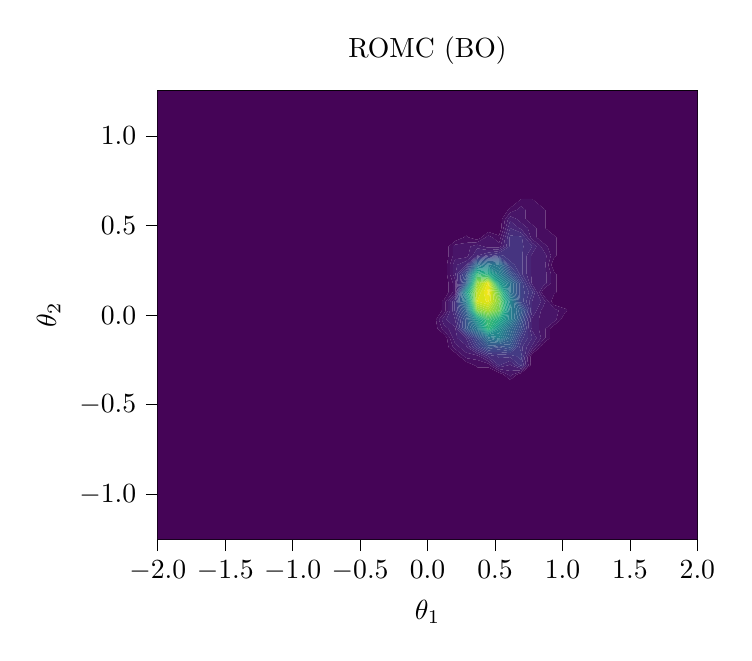
\begin{tikzpicture}

\definecolor{color0}{rgb}{0.269944,0.014625,0.341379}
\definecolor{color1}{rgb}{0.277018,0.050344,0.375715}
\definecolor{color2}{rgb}{0.281446,0.08432,0.407414}
\definecolor{color3}{rgb}{0.283197,0.11568,0.436115}
\definecolor{color4}{rgb}{0.28229,0.145912,0.46151}
\definecolor{color5}{rgb}{0.278826,0.17549,0.483397}
\definecolor{color6}{rgb}{0.273006,0.20452,0.501721}
\definecolor{color7}{rgb}{0.265145,0.232956,0.516599}
\definecolor{color8}{rgb}{0.255645,0.260703,0.528312}
\definecolor{color9}{rgb}{0.244972,0.287675,0.53726}
\definecolor{color10}{rgb}{0.233603,0.313828,0.543914}
\definecolor{color11}{rgb}{0.221989,0.339161,0.548752}
\definecolor{color12}{rgb}{0.210503,0.363727,0.552206}
\definecolor{color13}{rgb}{0.19943,0.387607,0.554642}
\definecolor{color14}{rgb}{0.188923,0.41091,0.556326}
\definecolor{color15}{rgb}{0.179019,0.433756,0.55743}
\definecolor{color16}{rgb}{0.169646,0.456262,0.55803}
\definecolor{color17}{rgb}{0.160665,0.47854,0.558115}
\definecolor{color18}{rgb}{0.151918,0.500685,0.557587}
\definecolor{color19}{rgb}{0.143343,0.522773,0.556295}
\definecolor{color20}{rgb}{0.135066,0.544853,0.554029}
\definecolor{color21}{rgb}{0.127568,0.566949,0.550556}
\definecolor{color22}{rgb}{0.122606,0.585371,0.546557}
\definecolor{color23}{rgb}{0.119512,0.607464,0.540218}
\definecolor{color24}{rgb}{0.12138,0.629492,0.531973}
\definecolor{color25}{rgb}{0.130067,0.651384,0.521608}
\definecolor{color26}{rgb}{0.146616,0.67305,0.508936}
\definecolor{color27}{rgb}{0.170948,0.694384,0.493803}
\definecolor{color28}{rgb}{0.202219,0.715272,0.476084}
\definecolor{color29}{rgb}{0.239374,0.735588,0.455688}
\definecolor{color30}{rgb}{0.281477,0.755203,0.432552}
\definecolor{color31}{rgb}{0.327796,0.77398,0.40664}
\definecolor{color32}{rgb}{0.377779,0.791781,0.377939}
\definecolor{color33}{rgb}{0.430983,0.808473,0.346476}
\definecolor{color34}{rgb}{0.487026,0.823929,0.312321}
\definecolor{color35}{rgb}{0.545524,0.838039,0.275626}
\definecolor{color36}{rgb}{0.606045,0.850733,0.236712}
\definecolor{color37}{rgb}{0.668054,0.861999,0.196293}
\definecolor{color38}{rgb}{0.730889,0.871916,0.156029}
\definecolor{color39}{rgb}{0.79376,0.880678,0.120005}
\definecolor{color40}{rgb}{0.85581,0.888601,0.097452}
\definecolor{color41}{rgb}{0.916242,0.896091,0.100717}
\definecolor{color42}{rgb}{0.974417,0.90359,0.130215}

\begin{axis}[
tick align=outside,
tick pos=left,
title={ROMC (BO)},
x grid style={white!69.0196078431373!black},
xlabel={\(\displaystyle \theta_1\)},
xmin=-2, xmax=2,
xtick style={color=black},
xtick={-2,-1.5,-1,-0.5,0,0.5,1,1.5,2},
xticklabels={
  \(\displaystyle {\ensuremath{-}2.0}\),
  \(\displaystyle {\ensuremath{-}1.5}\),
  \(\displaystyle {\ensuremath{-}1.0}\),
  \(\displaystyle {\ensuremath{-}0.5}\),
  \(\displaystyle {0.0}\),
  \(\displaystyle {0.5}\),
  \(\displaystyle {1.0}\),
  \(\displaystyle {1.5}\),
  \(\displaystyle {2.0}\)
},
y grid style={white!69.0196078431373!black},
ylabel={\(\displaystyle \theta_2\)},
ymin=-1.25, ymax=1.25,
ytick style={color=black},
ytick={-1.5,-1,-0.5,0,0.5,1,1.5},
yticklabels={
  \(\displaystyle {\ensuremath{-}1.5}\),
  \(\displaystyle {\ensuremath{-}1.0}\),
  \(\displaystyle {\ensuremath{-}0.5}\),
  \(\displaystyle {0.0}\),
  \(\displaystyle {0.5}\),
  \(\displaystyle {1.0}\),
  \(\displaystyle {1.5}\)
}
]
\addplot [draw=none, fill=color0]
table{%
x  y
-1.91836734693878 -1.25
-1.83673469387755 -1.25
-1.75510204081633 -1.25
-1.6734693877551 -1.25
-1.59183673469388 -1.25
-1.51020408163265 -1.25
-1.42857142857143 -1.25
-1.3469387755102 -1.25
-1.26530612244898 -1.25
-1.18367346938776 -1.25
-1.10204081632653 -1.25
-1.02040816326531 -1.25
-0.938775510204082 -1.25
-0.857142857142857 -1.25
-0.775510204081633 -1.25
-0.693877551020408 -1.25
-0.612244897959184 -1.25
-0.530612244897959 -1.25
-0.448979591836735 -1.25
-0.36734693877551 -1.25
-0.285714285714286 -1.25
-0.204081632653061 -1.25
-0.122448979591837 -1.25
-0.0408163265306123 -1.25
0.0408163265306123 -1.25
0.122448979591836 -1.25
0.204081632653061 -1.25
0.285714285714286 -1.25
0.36734693877551 -1.25
0.448979591836734 -1.25
0.530612244897959 -1.25
0.612244897959183 -1.25
0.693877551020408 -1.25
0.775510204081633 -1.25
0.857142857142857 -1.25
0.938775510204081 -1.25
1.02040816326531 -1.25
1.10204081632653 -1.25
1.18367346938775 -1.25
1.26530612244898 -1.25
1.3469387755102 -1.25
1.42857142857143 -1.25
1.51020408163265 -1.25
1.59183673469388 -1.25
1.6734693877551 -1.25
1.75510204081633 -1.25
1.83673469387755 -1.25
1.91836734693878 -1.25
2 -1.25
2 -1.19897959183673
2 -1.14795918367347
2 -1.0969387755102
2 -1.04591836734694
2 -0.994897959183674
2 -0.943877551020408
2 -0.892857142857143
2 -0.841836734693878
2 -0.790816326530612
2 -0.739795918367347
2 -0.688775510204082
2 -0.637755102040816
2 -0.586734693877551
2 -0.535714285714286
2 -0.48469387755102
2 -0.433673469387755
2 -0.38265306122449
2 -0.331632653061224
2 -0.280612244897959
2 -0.229591836734694
2 -0.178571428571429
2 -0.127551020408163
2 -0.0765306122448979
2 -0.0255102040816326
2 0.0255102040816326
2 0.0765306122448979
2 0.127551020408163
2 0.178571428571429
2 0.229591836734694
2 0.280612244897959
2 0.331632653061225
2 0.38265306122449
2 0.433673469387755
2 0.48469387755102
2 0.535714285714286
2 0.586734693877551
2 0.637755102040816
2 0.688775510204082
2 0.739795918367347
2 0.790816326530612
2 0.841836734693878
2 0.892857142857143
2 0.943877551020408
2 0.994897959183674
2 1.04591836734694
2 1.0969387755102
2 1.14795918367347
2 1.19897959183673
2 1.25
1.91836734693878 1.25
1.83673469387755 1.25
1.75510204081633 1.25
1.6734693877551 1.25
1.59183673469388 1.25
1.51020408163265 1.25
1.42857142857143 1.25
1.3469387755102 1.25
1.26530612244898 1.25
1.18367346938775 1.25
1.10204081632653 1.25
1.02040816326531 1.25
0.938775510204081 1.25
0.857142857142857 1.25
0.775510204081633 1.25
0.693877551020408 1.25
0.612244897959183 1.25
0.530612244897959 1.25
0.448979591836734 1.25
0.36734693877551 1.25
0.285714285714286 1.25
0.204081632653061 1.25
0.122448979591836 1.25
0.0408163265306123 1.25
-0.0408163265306123 1.25
-0.122448979591837 1.25
-0.204081632653061 1.25
-0.285714285714286 1.25
-0.36734693877551 1.25
-0.448979591836735 1.25
-0.530612244897959 1.25
-0.612244897959184 1.25
-0.693877551020408 1.25
-0.775510204081633 1.25
-0.857142857142857 1.25
-0.938775510204082 1.25
-1.02040816326531 1.25
-1.10204081632653 1.25
-1.18367346938776 1.25
-1.26530612244898 1.25
-1.3469387755102 1.25
-1.42857142857143 1.25
-1.51020408163265 1.25
-1.59183673469388 1.25
-1.6734693877551 1.25
-1.75510204081633 1.25
-1.83673469387755 1.25
-1.91836734693878 1.25
-2 1.25
-2 1.19897959183673
-2 1.14795918367347
-2 1.0969387755102
-2 1.04591836734694
-2 0.994897959183674
-2 0.943877551020408
-2 0.892857142857143
-2 0.841836734693878
-2 0.790816326530612
-2 0.739795918367347
-2 0.688775510204082
-2 0.637755102040816
-2 0.586734693877551
-2 0.535714285714286
-2 0.48469387755102
-2 0.433673469387755
-2 0.38265306122449
-2 0.331632653061225
-2 0.280612244897959
-2 0.229591836734694
-2 0.178571428571429
-2 0.127551020408163
-2 0.0765306122448979
-2 0.0255102040816326
-2 -0.0255102040816326
-2 -0.0765306122448979
-2 -0.127551020408163
-2 -0.178571428571429
-2 -0.229591836734694
-2 -0.280612244897959
-2 -0.331632653061224
-2 -0.38265306122449
-2 -0.433673469387755
-2 -0.48469387755102
-2 -0.535714285714286
-2 -0.586734693877551
-2 -0.637755102040816
-2 -0.688775510204082
-2 -0.739795918367347
-2 -0.790816326530612
-2 -0.841836734693878
-2 -0.892857142857143
-2 -0.943877551020408
-2 -0.994897959183674
-2 -1.04591836734694
-2 -1.0969387755102
-2 -1.14795918367347
-2 -1.19897959183673
-2 -1.25
-1.91836734693878 -1.25

0.563265306122449 -0.331632653061224
0.530612244897959 -0.321428571428571
0.448979591836734 -0.290816326530612
0.36734693877551 -0.290816326530612
0.351020408163265 -0.280612244897959
0.285714285714286 -0.260204081632653
0.236734693877551 -0.229591836734694
0.204081632653061 -0.209183673469388
0.155102040816326 -0.178571428571429
0.14421768707483 -0.127551020408163
0.122448979591836 -0.107142857142857
0.073469387755102 -0.0765306122448979
0.0625850340136054 -0.0255102040816326
0.106122448979592 0.0255102040816326
0.106122448979592 0.0765306122448979
0.122448979591836 0.086734693877551
0.155102040816326 0.127551020408163
0.155102040816326 0.178571428571429
0.14421768707483 0.229591836734694
0.14421768707483 0.280612244897959
0.155102040816326 0.331632653061225
0.155102040816326 0.38265306122449
0.204081632653061 0.413265306122449
0.269387755102041 0.433673469387755
0.285714285714286 0.443877551020408
0.302040816326531 0.433673469387755
0.36734693877551 0.420068027210884
0.4 0.433673469387755
0.448979591836734 0.464285714285714
0.530612244897959 0.443877551020408
0.546938775510204 0.48469387755102
0.552380952380952 0.535714285714286
0.595918367346939 0.586734693877551
0.612244897959183 0.596938775510204
0.677551020408163 0.637755102040816
0.693877551020408 0.647959183673469
0.775510204081633 0.647959183673469
0.791836734693877 0.637755102040816
0.857142857142857 0.596938775510204
0.873469387755102 0.586734693877551
0.873469387755102 0.535714285714286
0.873469387755102 0.48469387755102
0.938775510204081 0.443877551020408
0.955102040816326 0.433673469387755
0.955102040816326 0.38265306122449
0.955102040816326 0.331632653061225
0.938775510204081 0.321428571428572
0.917006802721088 0.280612244897959
0.938775510204081 0.239795918367347
0.955102040816326 0.229591836734694
0.955102040816326 0.178571428571429
0.955102040816326 0.127551020408163
0.938775510204081 0.11734693877551
0.917006802721088 0.0765306122448979
0.938775510204081 0.0561224489795918
1.02040816326531 0.0357142857142857
1.03673469387755 0.0255102040816326
1.02040816326531 0.0153061224489796
0.987755102040816 -0.0255102040816326
0.938775510204081 -0.0561224489795918
0.906122448979591 -0.0765306122448979
0.906122448979591 -0.127551020408163
0.857142857142857 -0.158163265306122
0.835374149659864 -0.178571428571429
0.775510204081633 -0.215986394557823
0.764625850340136 -0.229591836734694
0.762448979591837 -0.280612244897959
0.693877551020408 -0.323469387755102
0.661224489795918 -0.331632653061224
0.612244897959183 -0.362244897959184
0.563265306122449 -0.331632653061224
};
\addplot [draw=none, fill=color1]
table{%
x  y
0.612244897959183 -0.362244897959184
0.661224489795918 -0.331632653061224
0.693877551020408 -0.323469387755102
0.762448979591837 -0.280612244897959
0.764625850340136 -0.229591836734694
0.775510204081633 -0.215986394557823
0.835374149659864 -0.178571428571429
0.857142857142857 -0.158163265306122
0.906122448979591 -0.127551020408163
0.906122448979591 -0.0765306122448979
0.938775510204081 -0.0561224489795918
0.987755102040816 -0.0255102040816326
1.02040816326531 0.0153061224489796
1.03673469387755 0.0255102040816326
1.02040816326531 0.0357142857142857
0.938775510204081 0.0561224489795918
0.917006802721088 0.0765306122448979
0.938775510204081 0.11734693877551
0.955102040816326 0.127551020408163
0.955102040816326 0.178571428571429
0.955102040816326 0.229591836734694
0.938775510204081 0.239795918367347
0.917006802721088 0.280612244897959
0.938775510204081 0.321428571428572
0.955102040816326 0.331632653061225
0.955102040816326 0.38265306122449
0.955102040816326 0.433673469387755
0.938775510204081 0.443877551020408
0.873469387755102 0.48469387755102
0.873469387755102 0.535714285714286
0.873469387755102 0.586734693877551
0.857142857142857 0.596938775510204
0.791836734693877 0.637755102040816
0.775510204081633 0.647959183673469
0.693877551020408 0.647959183673469
0.677551020408163 0.637755102040816
0.612244897959183 0.596938775510204
0.595918367346939 0.586734693877551
0.552380952380952 0.535714285714286
0.546938775510204 0.48469387755102
0.530612244897959 0.443877551020408
0.448979591836734 0.464285714285714
0.4 0.433673469387755
0.36734693877551 0.420068027210884
0.302040816326531 0.433673469387755
0.285714285714286 0.443877551020408
0.269387755102041 0.433673469387755
0.204081632653061 0.413265306122449
0.155102040816326 0.38265306122449
0.155102040816326 0.331632653061225
0.14421768707483 0.280612244897959
0.14421768707483 0.229591836734694
0.155102040816326 0.178571428571429
0.155102040816326 0.127551020408163
0.122448979591836 0.086734693877551
0.106122448979592 0.0765306122448979
0.106122448979592 0.0255102040816326
0.0625850340136054 -0.0255102040816326
0.073469387755102 -0.0765306122448979
0.122448979591836 -0.107142857142857
0.14421768707483 -0.127551020408163
0.155102040816326 -0.178571428571429
0.204081632653061 -0.209183673469388
0.236734693877551 -0.229591836734694
0.285714285714286 -0.260204081632653
0.351020408163265 -0.280612244897959
0.36734693877551 -0.290816326530612
0.448979591836734 -0.290816326530612
0.530612244897959 -0.321428571428571
0.563265306122449 -0.331632653061224
0.612244897959183 -0.362244897959184

0.595918367346939 -0.331632653061224
0.530612244897959 -0.311224489795918
0.465306122448979 -0.280612244897959
0.448979591836734 -0.270408163265306
0.36734693877551 -0.25
0.285714285714286 -0.239795918367347
0.269387755102041 -0.229591836734694
0.204081632653061 -0.188775510204082
0.187755102040816 -0.178571428571429
0.165986394557823 -0.127551020408163
0.122448979591836 -0.0867346938775509
0.106122448979592 -0.0765306122448979
0.0843537414965985 -0.0255102040816326
0.122448979591836 0.010204081632653
0.13469387755102 0.0255102040816326
0.13469387755102 0.0765306122448979
0.187755102040816 0.127551020408163
0.187755102040816 0.178571428571429
0.165986394557823 0.229591836734694
0.165986394557823 0.280612244897959
0.187755102040816 0.331632653061225
0.187755102040816 0.38265306122449
0.204081632653061 0.392857142857143
0.285714285714286 0.403061224489796
0.36734693877551 0.406462585034014
0.432653061224489 0.433673469387755
0.448979591836734 0.443877551020408
0.481632653061224 0.433673469387755
0.530612244897959 0.403061224489796
0.542857142857143 0.433673469387755
0.563265306122449 0.48469387755102
0.574149659863945 0.535714285714286
0.612244897959183 0.571428571428571
0.661224489795918 0.586734693877551
0.693877551020408 0.607142857142857
0.726530612244898 0.586734693877551
0.726530612244898 0.535714285714286
0.775510204081633 0.505102040816326
0.808163265306122 0.48469387755102
0.808163265306122 0.433673469387755
0.857142857142857 0.403061224489796
0.889795918367347 0.38265306122449
0.914285714285714 0.331632653061225
0.895238095238095 0.280612244897959
0.914285714285714 0.229591836734694
0.914285714285714 0.178571428571429
0.857142857142857 0.142857142857143
0.844897959183673 0.127551020408163
0.857142857142857 0.112244897959184
0.895238095238095 0.0765306122448979
0.938775510204081 0.0357142857142857
0.971428571428571 0.0255102040816326
0.955102040816326 -0.0255102040816326
0.938775510204081 -0.0357142857142857
0.873469387755102 -0.0765306122448979
0.873469387755102 -0.127551020408163
0.857142857142857 -0.137755102040816
0.813605442176871 -0.178571428571429
0.775510204081633 -0.202380952380952
0.753741496598639 -0.229591836734694
0.749387755102041 -0.280612244897959
0.693877551020408 -0.31530612244898
0.628571428571428 -0.331632653061224
0.612244897959183 -0.341836734693878
0.595918367346939 -0.331632653061224
};
\addplot [draw=none, fill=color2]
table{%
x  y
0.612244897959183 -0.341836734693878
0.628571428571428 -0.331632653061224
0.693877551020408 -0.31530612244898
0.749387755102041 -0.280612244897959
0.753741496598639 -0.229591836734694
0.775510204081633 -0.202380952380952
0.813605442176871 -0.178571428571429
0.857142857142857 -0.137755102040816
0.873469387755102 -0.127551020408163
0.873469387755102 -0.0765306122448979
0.938775510204081 -0.0357142857142857
0.955102040816326 -0.0255102040816326
0.971428571428571 0.0255102040816326
0.938775510204081 0.0357142857142857
0.895238095238095 0.0765306122448979
0.857142857142857 0.112244897959184
0.844897959183673 0.127551020408163
0.857142857142857 0.142857142857143
0.914285714285714 0.178571428571429
0.914285714285714 0.229591836734694
0.895238095238095 0.280612244897959
0.914285714285714 0.331632653061225
0.889795918367347 0.38265306122449
0.857142857142857 0.403061224489796
0.808163265306122 0.433673469387755
0.808163265306122 0.48469387755102
0.775510204081633 0.505102040816326
0.726530612244898 0.535714285714286
0.726530612244898 0.586734693877551
0.693877551020408 0.607142857142857
0.661224489795918 0.586734693877551
0.612244897959183 0.571428571428571
0.574149659863945 0.535714285714286
0.563265306122449 0.48469387755102
0.542857142857143 0.433673469387755
0.530612244897959 0.403061224489796
0.481632653061224 0.433673469387755
0.448979591836734 0.443877551020408
0.432653061224489 0.433673469387755
0.36734693877551 0.406462585034014
0.285714285714286 0.403061224489796
0.204081632653061 0.392857142857143
0.187755102040816 0.38265306122449
0.187755102040816 0.331632653061225
0.165986394557823 0.280612244897959
0.165986394557823 0.229591836734694
0.187755102040816 0.178571428571429
0.187755102040816 0.127551020408163
0.13469387755102 0.0765306122448979
0.13469387755102 0.0255102040816326
0.122448979591836 0.010204081632653
0.0843537414965985 -0.0255102040816326
0.106122448979592 -0.0765306122448979
0.122448979591836 -0.0867346938775509
0.165986394557823 -0.127551020408163
0.187755102040816 -0.178571428571429
0.204081632653061 -0.188775510204082
0.269387755102041 -0.229591836734694
0.285714285714286 -0.239795918367347
0.36734693877551 -0.25
0.448979591836734 -0.270408163265306
0.465306122448979 -0.280612244897959
0.530612244897959 -0.311224489795918
0.595918367346939 -0.331632653061224
0.612244897959183 -0.341836734693878

0.487074829931972 -0.280612244897959
0.448979591836734 -0.256802721088435
0.383673469387755 -0.229591836734694
0.36734693877551 -0.224489795918367
0.285714285714286 -0.209183673469388
0.236734693877551 -0.178571428571429
0.204081632653061 -0.158163265306122
0.187755102040816 -0.127551020408163
0.155102040816326 -0.0765306122448979
0.122448979591836 -0.0561224489795918
0.106122448979592 -0.0255102040816326
0.122448979591836 -0.0102040816326531
0.151020408163265 0.0255102040816326
0.151020408163265 0.0765306122448979
0.204081632653061 0.120748299319728
0.206122448979592 0.127551020408163
0.208163265306122 0.178571428571429
0.204081632653061 0.198979591836735
0.187755102040816 0.229591836734694
0.187755102040816 0.280612244897959
0.204081632653061 0.311224489795918
0.285714285714286 0.321428571428572
0.302040816326531 0.331632653061225
0.318367346938775 0.38265306122449
0.36734693877551 0.392857142857143
0.416326530612245 0.38265306122449
0.448979591836734 0.375850340136055
0.530612244897959 0.377551020408163
0.541496598639456 0.38265306122449
0.559183673469387 0.433673469387755
0.579591836734694 0.48469387755102
0.595918367346939 0.535714285714286
0.612244897959183 0.551020408163265
0.661224489795918 0.535714285714286
0.693877551020408 0.51530612244898
0.742857142857143 0.48469387755102
0.764625850340136 0.433673469387755
0.775510204081633 0.423469387755102
0.840816326530612 0.38265306122449
0.857142857142857 0.362244897959184
0.881632653061224 0.331632653061225
0.873469387755102 0.280612244897959
0.881632653061224 0.229591836734694
0.881632653061224 0.178571428571429
0.857142857142857 0.163265306122449
0.828571428571428 0.127551020408163
0.857142857142857 0.0918367346938775
0.873469387755102 0.0765306122448979
0.857142857142857 0.0459183673469387
0.840816326530612 0.0255102040816326
0.824489795918367 -0.0255102040816326
0.824489795918367 -0.0765306122448979
0.840816326530612 -0.127551020408163
0.791836734693877 -0.178571428571429
0.775510204081633 -0.188775510204082
0.742857142857143 -0.229591836734694
0.736326530612245 -0.280612244897959
0.693877551020408 -0.307142857142857
0.612244897959183 -0.311224489795918
0.530612244897959 -0.301020408163265
0.487074829931972 -0.280612244897959
};
\addplot [draw=none, fill=color3]
table{%
x  y
0.530612244897959 -0.301020408163265
0.612244897959183 -0.311224489795918
0.693877551020408 -0.307142857142857
0.736326530612245 -0.280612244897959
0.742857142857143 -0.229591836734694
0.775510204081633 -0.188775510204082
0.791836734693877 -0.178571428571429
0.840816326530612 -0.127551020408163
0.824489795918367 -0.0765306122448979
0.824489795918367 -0.0255102040816326
0.840816326530612 0.0255102040816326
0.857142857142857 0.0459183673469387
0.873469387755102 0.0765306122448979
0.857142857142857 0.0918367346938775
0.828571428571428 0.127551020408163
0.857142857142857 0.163265306122449
0.881632653061224 0.178571428571429
0.881632653061224 0.229591836734694
0.873469387755102 0.280612244897959
0.881632653061224 0.331632653061225
0.857142857142857 0.362244897959184
0.840816326530612 0.38265306122449
0.775510204081633 0.423469387755102
0.764625850340136 0.433673469387755
0.742857142857143 0.48469387755102
0.693877551020408 0.51530612244898
0.661224489795918 0.535714285714286
0.612244897959183 0.551020408163265
0.595918367346939 0.535714285714286
0.579591836734694 0.48469387755102
0.559183673469387 0.433673469387755
0.541496598639456 0.38265306122449
0.530612244897959 0.377551020408163
0.448979591836734 0.375850340136054
0.416326530612245 0.38265306122449
0.36734693877551 0.392857142857143
0.318367346938775 0.38265306122449
0.302040816326531 0.331632653061225
0.285714285714286 0.321428571428572
0.204081632653061 0.311224489795918
0.187755102040816 0.280612244897959
0.187755102040816 0.229591836734694
0.204081632653061 0.198979591836735
0.208163265306122 0.178571428571429
0.206122448979592 0.127551020408163
0.204081632653061 0.120748299319728
0.151020408163265 0.0765306122448979
0.151020408163265 0.0255102040816326
0.122448979591836 -0.0102040816326531
0.106122448979592 -0.0255102040816326
0.122448979591836 -0.0561224489795918
0.155102040816326 -0.0765306122448979
0.187755102040816 -0.127551020408163
0.204081632653061 -0.158163265306122
0.236734693877551 -0.178571428571429
0.285714285714286 -0.209183673469388
0.36734693877551 -0.224489795918367
0.383673469387755 -0.229591836734694
0.448979591836734 -0.256802721088435
0.487074829931972 -0.280612244897959
0.530612244897959 -0.301020408163265

0.508843537414966 -0.280612244897959
0.448979591836734 -0.243197278911565
0.416326530612245 -0.229591836734694
0.36734693877551 -0.214285714285714
0.291156462585034 -0.178571428571429
0.285714285714286 -0.168367346938776
0.220408163265306 -0.127551020408163
0.206802721088435 -0.0765306122448979
0.204081632653061 -0.0663265306122448
0.138775510204081 -0.0255102040816326
0.16734693877551 0.0255102040816326
0.16734693877551 0.0765306122448979
0.204081632653061 0.107142857142857
0.210204081632653 0.127551020408163
0.216326530612245 0.178571428571429
0.20734693877551 0.229591836734694
0.220408163265306 0.280612244897959
0.285714285714286 0.301020408163265
0.33469387755102 0.331632653061225
0.36734693877551 0.372448979591837
0.448979591836734 0.362244897959184
0.530612244897959 0.36734693877551
0.563265306122449 0.38265306122449
0.575510204081632 0.433673469387755
0.595918367346939 0.48469387755102
0.612244897959183 0.525510204081633
0.677551020408163 0.48469387755102
0.693877551020408 0.479591836734694
0.742857142857143 0.433673469387755
0.775510204081633 0.403061224489796
0.808163265306122 0.38265306122449
0.775510204081633 0.341836734693878
0.76734693877551 0.331632653061225
0.76734693877551 0.280612244897959
0.76734693877551 0.229591836734694
0.771428571428571 0.178571428571429
0.775510204081633 0.173469387755102
0.812244897959183 0.127551020408163
0.840816326530612 0.0765306122448979
0.808163265306122 0.0255102040816326
0.775510204081633 -0.0153061224489796
0.772789115646259 -0.0255102040816326
0.772244897959184 -0.0765306122448979
0.775510204081633 -0.0867346938775509
0.808163265306122 -0.127551020408163
0.775510204081633 -0.168367346938776
0.76734693877551 -0.178571428571429
0.731972789115646 -0.229591836734694
0.723265306122449 -0.280612244897959
0.693877551020408 -0.298979591836735
0.620408163265306 -0.280612244897959
0.612244897959183 -0.275510204081633
0.595918367346938 -0.280612244897959
0.530612244897959 -0.290816326530612
0.508843537414966 -0.280612244897959
};
\addplot [draw=none, fill=color4]
table{%
x  y
0.530612244897959 -0.290816326530612
0.595918367346938 -0.280612244897959
0.612244897959183 -0.275510204081633
0.620408163265306 -0.280612244897959
0.693877551020408 -0.298979591836735
0.723265306122449 -0.280612244897959
0.731972789115646 -0.229591836734694
0.76734693877551 -0.178571428571429
0.775510204081633 -0.168367346938776
0.808163265306122 -0.127551020408163
0.775510204081633 -0.0867346938775509
0.772244897959184 -0.0765306122448979
0.772789115646259 -0.0255102040816326
0.775510204081633 -0.0153061224489796
0.808163265306122 0.0255102040816326
0.840816326530612 0.0765306122448979
0.812244897959183 0.127551020408163
0.775510204081633 0.173469387755102
0.771428571428571 0.178571428571429
0.76734693877551 0.229591836734694
0.76734693877551 0.280612244897959
0.76734693877551 0.331632653061225
0.775510204081633 0.341836734693878
0.808163265306122 0.38265306122449
0.775510204081633 0.403061224489796
0.742857142857143 0.433673469387755
0.693877551020408 0.479591836734694
0.677551020408163 0.48469387755102
0.612244897959183 0.525510204081633
0.595918367346939 0.48469387755102
0.575510204081632 0.433673469387755
0.563265306122449 0.38265306122449
0.530612244897959 0.36734693877551
0.448979591836734 0.362244897959184
0.36734693877551 0.372448979591837
0.33469387755102 0.331632653061225
0.285714285714286 0.301020408163265
0.220408163265306 0.280612244897959
0.20734693877551 0.229591836734694
0.216326530612245 0.178571428571429
0.210204081632653 0.127551020408163
0.204081632653061 0.107142857142857
0.16734693877551 0.0765306122448979
0.16734693877551 0.0255102040816326
0.138775510204081 -0.0255102040816326
0.204081632653061 -0.0663265306122448
0.206802721088435 -0.0765306122448979
0.220408163265306 -0.127551020408163
0.285714285714286 -0.168367346938776
0.291156462585034 -0.178571428571429
0.36734693877551 -0.214285714285714
0.416326530612245 -0.229591836734694
0.448979591836734 -0.243197278911565
0.508843537414966 -0.280612244897959
0.530612244897959 -0.290816326530612

0.653061224489796 -0.280612244897959
0.612244897959183 -0.255102040816326
0.530612244897959 -0.280612244897959
0.448979591836734 -0.229591836734694
0.36734693877551 -0.204081632653061
0.312925170068027 -0.178571428571429
0.285714285714286 -0.127551020408163
0.217687074829932 -0.0765306122448979
0.204081632653061 -0.0255102040816326
0.183673469387755 0.0255102040816326
0.183673469387755 0.0765306122448979
0.204081632653061 0.0935374149659864
0.214285714285714 0.127551020408163
0.224489795918367 0.178571428571429
0.220408163265306 0.229591836734694
0.285714285714286 0.280612244897959
0.36734693877551 0.331632653061225
0.36734693877551 0.331632653061225
0.448979591836734 0.348639455782313
0.530612244897959 0.357142857142857
0.585034013605442 0.38265306122449
0.591836734693877 0.433673469387755
0.612244897959183 0.48469387755102
0.693877551020408 0.459183673469388
0.72108843537415 0.433673469387755
0.775510204081633 0.38265306122449
0.73469387755102 0.331632653061225
0.73469387755102 0.280612244897959
0.73469387755102 0.229591836734694
0.755102040816326 0.178571428571429
0.775510204081633 0.153061224489796
0.795918367346939 0.127551020408163
0.775510204081633 0.0765306122448979
0.775510204081633 0.0255102040816326
0.761904761904762 -0.0255102040816326
0.759183673469388 -0.0765306122448979
0.775510204081633 -0.127551020408163
0.73469387755102 -0.178571428571429
0.72108843537415 -0.229591836734694
0.710204081632653 -0.280612244897959
0.693877551020408 -0.290816326530612
0.653061224489796 -0.280612244897959
};
\addplot [draw=none, fill=color5]
table{%
x  y
0.693877551020408 -0.290816326530612
0.710204081632653 -0.280612244897959
0.72108843537415 -0.229591836734694
0.73469387755102 -0.178571428571429
0.775510204081633 -0.127551020408163
0.759183673469388 -0.0765306122448979
0.761904761904762 -0.0255102040816326
0.775510204081633 0.0255102040816326
0.775510204081633 0.0765306122448979
0.795918367346939 0.127551020408163
0.775510204081633 0.153061224489796
0.755102040816326 0.178571428571429
0.73469387755102 0.229591836734694
0.73469387755102 0.280612244897959
0.73469387755102 0.331632653061225
0.775510204081633 0.38265306122449
0.72108843537415 0.433673469387755
0.693877551020408 0.459183673469388
0.612244897959183 0.48469387755102
0.591836734693877 0.433673469387755
0.585034013605442 0.38265306122449
0.530612244897959 0.357142857142857
0.448979591836734 0.348639455782313
0.36734693877551 0.331632653061225
0.36734693877551 0.331632653061225
0.285714285714286 0.280612244897959
0.220408163265306 0.229591836734694
0.224489795918367 0.178571428571429
0.214285714285714 0.127551020408163
0.204081632653061 0.0935374149659864
0.183673469387755 0.0765306122448979
0.183673469387755 0.0255102040816326
0.204081632653061 -0.0255102040816326
0.217687074829932 -0.0765306122448979
0.285714285714286 -0.127551020408163
0.312925170068027 -0.178571428571429
0.36734693877551 -0.204081632653061
0.448979591836734 -0.229591836734694
0.530612244897959 -0.280612244897959
0.612244897959183 -0.255102040816326
0.653061224489796 -0.280612244897959
0.693877551020408 -0.290816326530612

0.685714285714286 -0.280612244897959
0.612244897959183 -0.23469387755102
0.530612244897959 -0.239795918367347
0.514285714285714 -0.229591836734694
0.448979591836734 -0.221428571428571
0.36734693877551 -0.193877551020408
0.33469387755102 -0.178571428571429
0.302040816326531 -0.127551020408163
0.285714285714286 -0.119387755102041
0.228571428571428 -0.0765306122448979
0.217142857142857 -0.0255102040816326
0.204081632653061 0.0153061224489796
0.2 0.0255102040816326
0.2 0.0765306122448979
0.204081632653061 0.0799319727891156
0.218367346938775 0.127551020408163
0.23265306122449 0.178571428571429
0.233469387755102 0.229591836734694
0.285714285714286 0.270408163265306
0.293877551020408 0.280612244897959
0.36734693877551 0.326530612244898
0.43265306122449 0.331632653061225
0.448979591836734 0.335034013605442
0.530612244897959 0.346938775510204
0.606802721088435 0.38265306122449
0.608163265306122 0.433673469387755
0.612244897959183 0.443877551020408
0.693877551020408 0.438775510204082
0.699319727891156 0.433673469387755
0.710204081632653 0.38265306122449
0.70204081632653 0.331632653061225
0.70204081632653 0.280612244897959
0.70204081632653 0.229591836734694
0.738775510204082 0.178571428571429
0.775510204081633 0.13265306122449
0.779591836734694 0.127551020408163
0.775510204081633 0.11734693877551
0.75374149659864 0.0765306122448979
0.764625850340136 0.0255102040816326
0.751020408163265 -0.0255102040816326
0.746122448979592 -0.0765306122448979
0.742857142857143 -0.127551020408163
0.70204081632653 -0.178571428571429
0.710204081632653 -0.229591836734694
0.697142857142857 -0.280612244897959
0.693877551020408 -0.28265306122449
0.685714285714286 -0.280612244897959
};
\addplot [draw=none, fill=color6]
table{%
x  y
0.693877551020408 -0.28265306122449
0.697142857142857 -0.280612244897959
0.710204081632653 -0.229591836734694
0.70204081632653 -0.178571428571429
0.742857142857143 -0.127551020408163
0.746122448979592 -0.0765306122448979
0.751020408163265 -0.0255102040816326
0.764625850340136 0.0255102040816326
0.753741496598639 0.0765306122448979
0.775510204081633 0.11734693877551
0.779591836734694 0.127551020408163
0.775510204081633 0.13265306122449
0.738775510204082 0.178571428571429
0.70204081632653 0.229591836734694
0.70204081632653 0.280612244897959
0.70204081632653 0.331632653061225
0.710204081632653 0.38265306122449
0.699319727891156 0.433673469387755
0.693877551020408 0.438775510204082
0.612244897959183 0.443877551020408
0.608163265306122 0.433673469387755
0.606802721088435 0.38265306122449
0.530612244897959 0.346938775510204
0.448979591836734 0.335034013605442
0.43265306122449 0.331632653061225
0.36734693877551 0.326530612244898
0.293877551020408 0.280612244897959
0.285714285714286 0.270408163265306
0.233469387755102 0.229591836734694
0.23265306122449 0.178571428571429
0.218367346938775 0.127551020408163
0.204081632653061 0.0799319727891156
0.2 0.0765306122448979
0.2 0.0255102040816326
0.204081632653061 0.0153061224489796
0.217142857142857 -0.0255102040816326
0.228571428571428 -0.0765306122448979
0.285714285714286 -0.119387755102041
0.302040816326531 -0.127551020408163
0.33469387755102 -0.178571428571429
0.36734693877551 -0.193877551020408
0.448979591836734 -0.221428571428571
0.514285714285714 -0.229591836734694
0.530612244897959 -0.239795918367347
0.612244897959183 -0.23469387755102
0.685714285714286 -0.280612244897959
0.693877551020408 -0.28265306122449

0.661224489795918 -0.229591836734694
0.612244897959183 -0.221938775510204
0.530612244897959 -0.219387755102041
0.448979591836734 -0.213265306122449
0.36734693877551 -0.183673469387755
0.356462585034014 -0.178571428571429
0.318367346938775 -0.127551020408163
0.285714285714286 -0.111224489795918
0.239455782312925 -0.0765306122448979
0.230204081632653 -0.0255102040816326
0.212244897959183 0.0255102040816326
0.208979591836734 0.0765306122448979
0.222448979591837 0.127551020408163
0.240816326530612 0.178571428571429
0.246530612244898 0.229591836734694
0.285714285714286 0.260204081632653
0.302040816326531 0.280612244897959
0.36734693877551 0.321428571428572
0.448979591836734 0.328231292517007
0.497959183673469 0.331632653061225
0.530612244897959 0.336734693877551
0.563265306122449 0.331632653061225
0.612244897959183 0.301020408163265
0.644897959183673 0.280612244897959
0.681632653061224 0.229591836734694
0.693877551020408 0.214285714285714
0.722448979591837 0.178571428571429
0.751020408163265 0.127551020408163
0.731972789115646 0.0765306122448979
0.753741496598639 0.0255102040816326
0.740136054421769 -0.0255102040816326
0.733061224489796 -0.0765306122448979
0.710204081632653 -0.127551020408163
0.693877551020408 -0.147959183673469
0.681632653061224 -0.178571428571429
0.693877551020408 -0.209183673469388
0.699319727891156 -0.229591836734694
0.693877551020408 -0.25
0.661224489795918 -0.229591836734694
};
\addplot [draw=none, fill=color7]
table{%
x  y
0.693877551020408 -0.25
0.699319727891156 -0.229591836734694
0.693877551020408 -0.209183673469388
0.681632653061224 -0.178571428571429
0.693877551020408 -0.147959183673469
0.710204081632653 -0.127551020408163
0.733061224489796 -0.0765306122448979
0.740136054421769 -0.0255102040816326
0.753741496598639 0.0255102040816326
0.731972789115646 0.0765306122448979
0.751020408163265 0.127551020408163
0.722448979591837 0.178571428571429
0.693877551020408 0.214285714285714
0.681632653061224 0.229591836734694
0.644897959183673 0.280612244897959
0.612244897959183 0.301020408163265
0.563265306122449 0.331632653061225
0.530612244897959 0.336734693877551
0.497959183673469 0.331632653061225
0.448979591836734 0.328231292517007
0.36734693877551 0.321428571428572
0.302040816326531 0.280612244897959
0.285714285714286 0.260204081632653
0.246530612244898 0.229591836734694
0.240816326530612 0.178571428571429
0.222448979591837 0.127551020408163
0.208979591836735 0.0765306122448979
0.212244897959183 0.0255102040816326
0.230204081632653 -0.0255102040816326
0.239455782312925 -0.0765306122448979
0.285714285714286 -0.111224489795918
0.318367346938775 -0.127551020408163
0.356462585034014 -0.178571428571429
0.36734693877551 -0.183673469387755
0.448979591836734 -0.213265306122449
0.530612244897959 -0.219387755102041
0.612244897959183 -0.221938775510204
0.661224489795918 -0.229591836734694
0.693877551020408 -0.25

0.378231292517007 -0.178571428571429
0.36734693877551 -0.168367346938775
0.33469387755102 -0.127551020408163
0.285714285714286 -0.103061224489796
0.250340136054422 -0.0765306122448979
0.243265306122449 -0.0255102040816326
0.22312925170068 0.0255102040816326
0.215510204081632 0.0765306122448979
0.226530612244898 0.127551020408163
0.248979591836735 0.178571428571429
0.259591836734694 0.229591836734694
0.285714285714286 0.25
0.310204081632653 0.280612244897959
0.36734693877551 0.316326530612245
0.448979591836734 0.323696145124717
0.530612244897959 0.328717201166181
0.607580174927114 0.280612244897959
0.612244897959183 0.273809523809524
0.665306122448979 0.229591836734694
0.693877551020408 0.193877551020408
0.706122448979592 0.178571428571429
0.718367346938775 0.127551020408163
0.710204081632653 0.0765306122448979
0.742857142857143 0.0255102040816326
0.729251700680272 -0.0255102040816326
0.72 -0.0765306122448979
0.693877551020408 -0.11734693877551
0.68734693877551 -0.127551020408163
0.665306122448979 -0.178571428571429
0.612244897959183 -0.211734693877551
0.530612244897959 -0.20578231292517
0.448979591836734 -0.205102040816327
0.378231292517007 -0.178571428571429
};
\addplot [draw=none, fill=color8]
table{%
x  y
0.448979591836734 -0.205102040816327
0.530612244897959 -0.20578231292517
0.612244897959183 -0.211734693877551
0.665306122448979 -0.178571428571429
0.68734693877551 -0.127551020408163
0.693877551020408 -0.11734693877551
0.72 -0.0765306122448979
0.729251700680272 -0.0255102040816326
0.742857142857143 0.0255102040816326
0.710204081632653 0.0765306122448979
0.718367346938775 0.127551020408163
0.706122448979592 0.178571428571429
0.693877551020408 0.193877551020408
0.665306122448979 0.229591836734694
0.612244897959183 0.273809523809524
0.607580174927114 0.280612244897959
0.530612244897959 0.328717201166181
0.448979591836734 0.323696145124717
0.36734693877551 0.316326530612245
0.310204081632653 0.280612244897959
0.285714285714286 0.25
0.259591836734694 0.229591836734694
0.248979591836735 0.178571428571429
0.226530612244898 0.127551020408163
0.215510204081632 0.0765306122448979
0.22312925170068 0.0255102040816326
0.243265306122449 -0.0255102040816326
0.250340136054422 -0.0765306122448979
0.285714285714286 -0.103061224489796
0.33469387755102 -0.127551020408163
0.36734693877551 -0.168367346938775
0.378231292517007 -0.178571428571429
0.448979591836734 -0.205102040816327

0.4 -0.178571428571429
0.36734693877551 -0.147959183673469
0.351020408163265 -0.127551020408163
0.285714285714286 -0.0948979591836734
0.261224489795918 -0.0765306122448979
0.256326530612245 -0.0255102040816326
0.234013605442177 0.0255102040816326
0.22204081632653 0.0765306122448979
0.230612244897959 0.127551020408163
0.257142857142857 0.178571428571429
0.27265306122449 0.229591836734694
0.285714285714286 0.239795918367347
0.318367346938775 0.280612244897959
0.36734693877551 0.311224489795918
0.448979591836734 0.319160997732426
0.530612244897959 0.322886297376093
0.598250728862973 0.280612244897959
0.612244897959183 0.260204081632653
0.648979591836734 0.229591836734694
0.691156462585034 0.178571428571429
0.691156462585034 0.127551020408163
0.692063492063492 0.0765306122448979
0.693877551020408 0.0731292517006802
0.731972789115646 0.0255102040816326
0.718367346938775 -0.0255102040816326
0.706938775510204 -0.0765306122448979
0.693877551020408 -0.096938775510204
0.674285714285714 -0.127551020408163
0.648979591836734 -0.178571428571429
0.612244897959183 -0.201530612244898
0.530612244897959 -0.192176870748299
0.448979591836734 -0.196938775510204
0.4 -0.178571428571429
};
\addplot [draw=none, fill=color9]
table{%
x  y
0.448979591836734 -0.196938775510204
0.530612244897959 -0.192176870748299
0.612244897959183 -0.201530612244898
0.648979591836734 -0.178571428571429
0.674285714285714 -0.127551020408163
0.693877551020408 -0.096938775510204
0.706938775510204 -0.0765306122448979
0.718367346938775 -0.0255102040816326
0.731972789115646 0.0255102040816326
0.693877551020408 0.0731292517006802
0.692063492063492 0.0765306122448979
0.691156462585034 0.127551020408163
0.691156462585034 0.178571428571429
0.648979591836734 0.229591836734694
0.612244897959183 0.260204081632653
0.598250728862973 0.280612244897959
0.530612244897959 0.322886297376093
0.448979591836734 0.319160997732426
0.36734693877551 0.311224489795918
0.318367346938775 0.280612244897959
0.285714285714286 0.239795918367347
0.27265306122449 0.229591836734694
0.257142857142857 0.178571428571429
0.230612244897959 0.127551020408163
0.22204081632653 0.0765306122448979
0.234013605442177 0.0255102040816326
0.256326530612245 -0.0255102040816326
0.261224489795918 -0.0765306122448979
0.285714285714286 -0.0948979591836734
0.351020408163265 -0.127551020408163
0.36734693877551 -0.147959183673469
0.4 -0.178571428571429
0.448979591836734 -0.196938775510204

0.421768707482993 -0.178571428571429
0.36734693877551 -0.127551020408163
0.36734693877551 -0.127551020408163
0.285714285714286 -0.0867346938775509
0.272108843537415 -0.0765306122448979
0.269387755102041 -0.0255102040816326
0.244897959183673 0.0255102040816326
0.228571428571428 0.0765306122448979
0.23469387755102 0.127551020408163
0.265306122448979 0.178571428571429
0.285714285714286 0.229591836734694
0.326530612244898 0.280612244897959
0.36734693877551 0.306122448979592
0.448979591836734 0.314625850340136
0.530612244897959 0.317055393586006
0.588921282798834 0.280612244897959
0.612244897959183 0.246598639455782
0.63265306122449 0.229591836734694
0.680272108843537 0.178571428571429
0.680272108843537 0.127551020408163
0.684807256235827 0.0765306122448979
0.693877551020408 0.0595238095238095
0.72108843537415 0.0255102040816326
0.707482993197279 -0.0255102040816326
0.693877551020408 -0.0765306122448979
0.661224489795918 -0.127551020408163
0.63265306122449 -0.178571428571429
0.612244897959183 -0.191326530612245
0.530612244897959 -0.178571428571429
0.448979591836734 -0.188775510204082
0.421768707482993 -0.178571428571429
};
\addplot [draw=none, fill=color10]
table{%
x  y
0.448979591836734 -0.188775510204082
0.530612244897959 -0.178571428571429
0.612244897959183 -0.191326530612245
0.63265306122449 -0.178571428571429
0.661224489795918 -0.127551020408163
0.693877551020408 -0.0765306122448979
0.707482993197279 -0.0255102040816326
0.72108843537415 0.0255102040816326
0.693877551020408 0.0595238095238095
0.684807256235827 0.0765306122448979
0.680272108843537 0.127551020408163
0.680272108843537 0.178571428571429
0.63265306122449 0.229591836734694
0.612244897959183 0.246598639455782
0.588921282798834 0.280612244897959
0.530612244897959 0.317055393586006
0.448979591836734 0.314625850340136
0.36734693877551 0.306122448979592
0.326530612244898 0.280612244897959
0.285714285714286 0.229591836734694
0.265306122448979 0.178571428571429
0.23469387755102 0.127551020408163
0.228571428571428 0.0765306122448979
0.244897959183673 0.0255102040816326
0.269387755102041 -0.0255102040816326
0.272108843537415 -0.0765306122448979
0.285714285714286 -0.0867346938775509
0.36734693877551 -0.127551020408163
0.36734693877551 -0.127551020408163
0.421768707482993 -0.178571428571429
0.448979591836734 -0.188775510204082

0.443537414965986 -0.178571428571429
0.380408163265306 -0.127551020408163
0.36734693877551 -0.120748299319728
0.285714285714286 -0.0785714285714285
0.282993197278911 -0.0765306122448979
0.282448979591837 -0.0255102040816326
0.25578231292517 0.0255102040816326
0.235102040816326 0.0765306122448979
0.238775510204081 0.127551020408163
0.273469387755102 0.178571428571429
0.285714285714286 0.209183673469388
0.290068027210884 0.229591836734694
0.33469387755102 0.280612244897959
0.36734693877551 0.301020408163265
0.448979591836734 0.310090702947846
0.530612244897959 0.311224489795918
0.579591836734694 0.280612244897959
0.612244897959183 0.232993197278912
0.616326530612245 0.229591836734694
0.669387755102041 0.178571428571429
0.669387755102041 0.127551020408163
0.677551020408163 0.0765306122448979
0.693877551020408 0.0459183673469387
0.710204081632653 0.0255102040816326
0.696598639455782 -0.0255102040816326
0.693877551020408 -0.0357142857142856
0.677551020408163 -0.0765306122448979
0.648163265306122 -0.127551020408163
0.616326530612245 -0.178571428571429
0.612244897959183 -0.181122448979592
0.595918367346939 -0.178571428571429
0.530612244897959 -0.172740524781341
0.465306122448979 -0.178571428571429
0.448979591836734 -0.180612244897959
0.443537414965986 -0.178571428571429
};
\addplot [draw=none, fill=color11]
table{%
x  y
0.448979591836734 -0.180612244897959
0.465306122448979 -0.178571428571429
0.530612244897959 -0.172740524781341
0.595918367346939 -0.178571428571429
0.612244897959183 -0.181122448979592
0.616326530612245 -0.178571428571429
0.648163265306122 -0.127551020408163
0.677551020408163 -0.0765306122448979
0.693877551020408 -0.0357142857142856
0.696598639455782 -0.0255102040816326
0.710204081632653 0.0255102040816326
0.693877551020408 0.0459183673469387
0.677551020408163 0.0765306122448979
0.669387755102041 0.127551020408163
0.669387755102041 0.178571428571429
0.616326530612245 0.229591836734694
0.612244897959183 0.232993197278912
0.579591836734694 0.280612244897959
0.530612244897959 0.311224489795918
0.448979591836734 0.310090702947846
0.36734693877551 0.301020408163265
0.33469387755102 0.280612244897959
0.290068027210884 0.229591836734694
0.285714285714286 0.209183673469388
0.273469387755102 0.178571428571429
0.238775510204081 0.127551020408163
0.235102040816326 0.0765306122448979
0.25578231292517 0.0255102040816326
0.282448979591837 -0.0255102040816326
0.282993197278911 -0.0765306122448979
0.285714285714286 -0.0785714285714285
0.36734693877551 -0.120748299319728
0.380408163265306 -0.127551020408163
0.443537414965986 -0.178571428571429
0.448979591836734 -0.180612244897959

0.393469387755102 -0.127551020408163
0.36734693877551 -0.113945578231292
0.295510204081633 -0.0765306122448979
0.291156462585034 -0.0255102040816326
0.285714285714286 -0.010204081632653
0.266666666666667 0.0255102040816326
0.241632653061224 0.0765306122448979
0.242857142857143 0.127551020408163
0.281632653061224 0.178571428571429
0.285714285714286 0.188775510204082
0.294421768707483 0.229591836734694
0.342857142857143 0.280612244897959
0.36734693877551 0.295918367346939
0.448979591836734 0.305555555555556
0.530612244897959 0.305393586005831
0.570262390670554 0.280612244897959
0.604081632653061 0.229591836734694
0.612244897959183 0.221938775510204
0.658503401360544 0.178571428571429
0.658503401360544 0.127551020408163
0.670294784580499 0.0765306122448979
0.693877551020408 0.032312925170068
0.699319727891156 0.0255102040816326
0.693877551020408 0.0051020408163266
0.685714285714286 -0.0255102040816326
0.661224489795918 -0.0765306122448979
0.635102040816326 -0.127551020408163
0.612244897959183 -0.163265306122449
0.530612244897959 -0.166909620991254
0.448979591836734 -0.170918367346939
0.393469387755102 -0.127551020408163
};
\addplot [draw=none, fill=color12]
table{%
x  y
0.448979591836734 -0.170918367346939
0.530612244897959 -0.166909620991254
0.612244897959183 -0.163265306122449
0.635102040816326 -0.127551020408163
0.661224489795918 -0.0765306122448979
0.685714285714285 -0.0255102040816326
0.693877551020408 0.0051020408163266
0.699319727891156 0.0255102040816326
0.693877551020408 0.032312925170068
0.670294784580499 0.0765306122448979
0.658503401360544 0.127551020408163
0.658503401360544 0.178571428571429
0.612244897959183 0.221938775510204
0.604081632653061 0.229591836734694
0.570262390670554 0.280612244897959
0.530612244897959 0.305393586005831
0.448979591836734 0.305555555555556
0.36734693877551 0.295918367346939
0.342857142857143 0.280612244897959
0.294421768707483 0.229591836734694
0.285714285714286 0.188775510204082
0.281632653061224 0.178571428571429
0.242857142857143 0.127551020408163
0.241632653061224 0.0765306122448979
0.266666666666667 0.0255102040816326
0.285714285714286 -0.010204081632653
0.291156462585034 -0.0255102040816326
0.295510204081633 -0.0765306122448979
0.36734693877551 -0.113945578231292
0.393469387755102 -0.127551020408163
0.448979591836734 -0.170918367346939

0.406530612244898 -0.127551020408163
0.36734693877551 -0.107142857142857
0.308571428571428 -0.0765306122448979
0.298412698412698 -0.0255102040816326
0.285714285714286 0.0102040816326531
0.277551020408163 0.0255102040816326
0.248163265306122 0.0765306122448979
0.246938775510204 0.127551020408163
0.285714285714286 0.176020408163265
0.287432867883996 0.178571428571429
0.298775510204082 0.229591836734694
0.351020408163265 0.280612244897959
0.36734693877551 0.290816326530612
0.448979591836734 0.301020408163265
0.530612244897959 0.299562682215744
0.560932944606414 0.280612244897959
0.593197278911564 0.229591836734694
0.612244897959183 0.211734693877551
0.647619047619047 0.178571428571429
0.647619047619047 0.127551020408163
0.663038548752834 0.0765306122448979
0.68734693877551 0.0255102040816326
0.674829931972789 -0.0255102040816326
0.644897959183673 -0.0765306122448979
0.62204081632653 -0.127551020408163
0.612244897959183 -0.142857142857143
0.530612244897959 -0.161078717201166
0.448979591836734 -0.160714285714286
0.406530612244898 -0.127551020408163
};
\addplot [draw=none, fill=color13]
table{%
x  y
0.448979591836734 -0.160714285714286
0.530612244897959 -0.161078717201166
0.612244897959183 -0.142857142857143
0.62204081632653 -0.127551020408163
0.644897959183673 -0.0765306122448979
0.674829931972789 -0.0255102040816326
0.68734693877551 0.0255102040816326
0.663038548752834 0.0765306122448979
0.647619047619047 0.127551020408163
0.647619047619047 0.178571428571429
0.612244897959183 0.211734693877551
0.593197278911564 0.229591836734694
0.560932944606414 0.280612244897959
0.530612244897959 0.299562682215744
0.448979591836734 0.301020408163265
0.36734693877551 0.290816326530612
0.351020408163265 0.280612244897959
0.298775510204081 0.229591836734694
0.287432867883996 0.178571428571429
0.285714285714286 0.176020408163265
0.246938775510204 0.127551020408163
0.248163265306122 0.0765306122448979
0.277551020408163 0.0255102040816326
0.285714285714286 0.0102040816326531
0.298412698412698 -0.0255102040816326
0.308571428571428 -0.0765306122448979
0.36734693877551 -0.107142857142857
0.406530612244898 -0.127551020408163
0.448979591836734 -0.160714285714286

0.419591836734694 -0.127551020408163
0.36734693877551 -0.100340136054422
0.321632653061224 -0.0765306122448979
0.305668934240363 -0.0255102040816326
0.286674669867947 0.0255102040816326
0.285714285714286 0.0280612244897959
0.25469387755102 0.0765306122448979
0.251020408163265 0.127551020408163
0.285714285714286 0.170918367346939
0.290870032223416 0.178571428571429
0.30312925170068 0.229591836734694
0.359183673469388 0.280612244897959
0.36734693877551 0.285714285714286
0.448979591836734 0.296485260770975
0.530612244897959 0.293731778425656
0.551603498542274 0.280612244897959
0.582312925170068 0.229591836734694
0.612244897959183 0.201530612244898
0.636734693877551 0.178571428571429
0.636734693877551 0.127551020408163
0.65578231292517 0.0765306122448979
0.674285714285714 0.0255102040816326
0.663945578231292 -0.0255102040816326
0.628571428571428 -0.0765306122448979
0.612244897959183 -0.11734693877551
0.608163265306122 -0.127551020408163
0.530612244897959 -0.155247813411079
0.448979591836734 -0.150510204081633
0.419591836734694 -0.127551020408163
};
\addplot [draw=none, fill=color14]
table{%
x  y
0.448979591836734 -0.150510204081633
0.530612244897959 -0.155247813411079
0.608163265306122 -0.127551020408163
0.612244897959183 -0.11734693877551
0.628571428571428 -0.0765306122448979
0.663945578231292 -0.0255102040816326
0.674285714285714 0.0255102040816326
0.65578231292517 0.0765306122448979
0.636734693877551 0.127551020408163
0.636734693877551 0.178571428571429
0.612244897959183 0.201530612244898
0.582312925170068 0.229591836734694
0.551603498542274 0.280612244897959
0.530612244897959 0.293731778425656
0.448979591836734 0.296485260770975
0.36734693877551 0.285714285714286
0.359183673469388 0.280612244897959
0.30312925170068 0.229591836734694
0.290870032223416 0.178571428571429
0.285714285714286 0.170918367346939
0.251020408163265 0.127551020408163
0.25469387755102 0.0765306122448979
0.285714285714286 0.0280612244897959
0.286674669867947 0.0255102040816326
0.305668934240363 -0.0255102040816326
0.321632653061224 -0.0765306122448979
0.36734693877551 -0.100340136054422
0.419591836734694 -0.127551020408163
0.448979591836734 -0.150510204081633

0.432653061224489 -0.127551020408163
0.36734693877551 -0.0935374149659863
0.33469387755102 -0.0765306122448979
0.312925170068027 -0.0255102040816326
0.290516206482593 0.0255102040816326
0.285714285714286 0.0382653061224489
0.261224489795918 0.0765306122448979
0.255102040816326 0.127551020408163
0.285714285714286 0.165816326530612
0.294307196562836 0.178571428571429
0.307482993197279 0.229591836734694
0.36734693877551 0.280612244897959
0.36734693877551 0.280612244897959
0.448979591836734 0.291950113378685
0.530612244897959 0.287900874635569
0.542274052478134 0.280612244897959
0.571428571428571 0.229591836734694
0.612244897959183 0.191326530612245
0.625850340136054 0.178571428571429
0.625850340136054 0.127551020408163
0.648526077097505 0.0765306122448979
0.661224489795918 0.0255102040816326
0.653061224489796 -0.0255102040816326
0.612244897959183 -0.0765306122448979
0.591836734693877 -0.127551020408163
0.530612244897959 -0.149416909620991
0.448979591836734 -0.140306122448979
0.432653061224489 -0.127551020408163
};
\addplot [draw=none, fill=color15]
table{%
x  y
0.448979591836734 -0.140306122448979
0.530612244897959 -0.149416909620991
0.591836734693877 -0.127551020408163
0.612244897959183 -0.0765306122448979
0.653061224489796 -0.0255102040816326
0.661224489795918 0.0255102040816326
0.648526077097505 0.0765306122448979
0.625850340136054 0.127551020408163
0.625850340136054 0.178571428571429
0.612244897959183 0.191326530612245
0.571428571428571 0.229591836734694
0.542274052478134 0.280612244897959
0.530612244897959 0.287900874635569
0.448979591836734 0.291950113378685
0.36734693877551 0.280612244897959
0.36734693877551 0.280612244897959
0.307482993197279 0.229591836734694
0.294307196562836 0.178571428571429
0.285714285714286 0.165816326530612
0.255102040816326 0.127551020408163
0.261224489795918 0.0765306122448979
0.285714285714286 0.0382653061224489
0.290516206482593 0.0255102040816326
0.312925170068027 -0.0255102040816326
0.33469387755102 -0.0765306122448979
0.36734693877551 -0.0935374149659863
0.432653061224489 -0.127551020408163
0.448979591836734 -0.140306122448979

0.445714285714285 -0.127551020408163
0.36734693877551 -0.0867346938775509
0.347755102040816 -0.0765306122448979
0.320181405895692 -0.0255102040816326
0.294357743097239 0.0255102040816326
0.285714285714286 0.048469387755102
0.267755102040816 0.0765306122448979
0.259183673469388 0.127551020408163
0.285714285714286 0.160714285714286
0.297744360902256 0.178571428571429
0.311836734693877 0.229591836734694
0.36734693877551 0.276901669758813
0.4 0.280612244897959
0.448979591836734 0.287414965986395
0.530612244897959 0.282069970845481
0.532944606413994 0.280612244897959
0.560544217687075 0.229591836734694
0.612244897959183 0.181122448979592
0.614965986394558 0.178571428571429
0.614965986394558 0.127551020408163
0.641269841269841 0.0765306122448979
0.648163265306122 0.0255102040816326
0.642176870748299 -0.0255102040816326
0.612244897959183 -0.0629251700680271
0.599183673469388 -0.0765306122448979
0.575510204081632 -0.127551020408163
0.530612244897959 -0.143586005830904
0.448979591836734 -0.130102040816326
0.445714285714285 -0.127551020408163
};
\addplot [draw=none, fill=color16]
table{%
x  y
0.448979591836734 -0.130102040816326
0.530612244897959 -0.143586005830904
0.575510204081632 -0.127551020408163
0.599183673469388 -0.0765306122448979
0.612244897959183 -0.0629251700680271
0.642176870748299 -0.0255102040816326
0.648163265306122 0.0255102040816326
0.641269841269841 0.0765306122448979
0.614965986394558 0.127551020408163
0.614965986394558 0.178571428571429
0.612244897959183 0.181122448979592
0.560544217687075 0.229591836734694
0.532944606413994 0.280612244897959
0.530612244897959 0.282069970845481
0.448979591836734 0.287414965986395
0.4 0.280612244897959
0.36734693877551 0.276901669758813
0.311836734693877 0.229591836734694
0.297744360902256 0.178571428571429
0.285714285714286 0.160714285714286
0.259183673469388 0.127551020408163
0.267755102040816 0.0765306122448979
0.285714285714286 0.048469387755102
0.294357743097239 0.0255102040816326
0.320181405895692 -0.0255102040816326
0.347755102040816 -0.0765306122448979
0.36734693877551 -0.0867346938775509
0.445714285714285 -0.127551020408163
0.448979591836734 -0.130102040816326

0.473469387755102 -0.127551020408163
0.448979591836734 -0.124489795918367
0.36734693877551 -0.0799319727891155
0.360816326530612 -0.0765306122448979
0.327437641723356 -0.0255102040816326
0.298199279711885 0.0255102040816326
0.285714285714286 0.0586734693877551
0.274285714285714 0.0765306122448979
0.263265306122449 0.127551020408163
0.285714285714286 0.155612244897959
0.301181525241676 0.178571428571429
0.316190476190476 0.229591836734694
0.36734693877551 0.273191094619666
0.43265306122449 0.280612244897959
0.448979591836734 0.282879818594104
0.481632653061224 0.280612244897959
0.530612244897959 0.26530612244898
0.549659863945578 0.229591836734694
0.604081632653061 0.178571428571429
0.608477237048665 0.127551020408163
0.612244897959183 0.11734693877551
0.634013605442177 0.0765306122448979
0.635102040816326 0.0255102040816326
0.631292517006803 -0.0255102040816326
0.612244897959183 -0.0493197278911564
0.586122448979592 -0.0765306122448979
0.559183673469387 -0.127551020408163
0.530612244897959 -0.137755102040816
0.473469387755102 -0.127551020408163
};
\addplot [draw=none, fill=color17]
table{%
x  y
0.530612244897959 -0.137755102040816
0.559183673469387 -0.127551020408163
0.586122448979592 -0.0765306122448979
0.612244897959183 -0.0493197278911564
0.631292517006803 -0.0255102040816326
0.635102040816326 0.0255102040816326
0.634013605442177 0.0765306122448979
0.612244897959183 0.11734693877551
0.608477237048665 0.127551020408163
0.604081632653061 0.178571428571429
0.549659863945578 0.229591836734694
0.530612244897959 0.26530612244898
0.481632653061224 0.280612244897959
0.448979591836734 0.282879818594104
0.43265306122449 0.280612244897959
0.36734693877551 0.273191094619666
0.316190476190476 0.229591836734694
0.301181525241676 0.178571428571429
0.285714285714286 0.155612244897959
0.263265306122449 0.127551020408163
0.274285714285714 0.0765306122448979
0.285714285714286 0.0586734693877551
0.298199279711885 0.0255102040816326
0.327437641723356 -0.0255102040816326
0.360816326530612 -0.0765306122448979
0.36734693877551 -0.0799319727891155
0.448979591836734 -0.124489795918367
0.473469387755102 -0.127551020408163
0.530612244897959 -0.137755102040816

0.506122448979592 -0.127551020408163
0.448979591836734 -0.120408163265306
0.370975056689342 -0.0765306122448979
0.36734693877551 -0.0714285714285713
0.33469387755102 -0.0255102040816326
0.302040816326531 0.0255102040816326
0.285714285714286 0.0688775510204081
0.280816326530612 0.0765306122448979
0.26734693877551 0.127551020408163
0.285714285714286 0.150510204081633
0.304618689581096 0.178571428571429
0.320544217687075 0.229591836734694
0.36734693877551 0.26948051948052
0.448979591836734 0.277696793002916
0.530612244897959 0.244897959183673
0.538775510204081 0.229591836734694
0.593197278911564 0.178571428571429
0.603453689167975 0.127551020408163
0.612244897959183 0.103741496598639
0.626757369614512 0.0765306122448979
0.62204081632653 0.0255102040816326
0.620408163265306 -0.0255102040816326
0.612244897959183 -0.0357142857142857
0.573061224489796 -0.0765306122448979
0.542857142857143 -0.127551020408163
0.530612244897959 -0.131924198250729
0.506122448979592 -0.127551020408163
};
\addplot [draw=none, fill=color18]
table{%
x  y
0.530612244897959 -0.131924198250729
0.542857142857143 -0.127551020408163
0.573061224489796 -0.0765306122448979
0.612244897959183 -0.0357142857142857
0.620408163265306 -0.0255102040816326
0.62204081632653 0.0255102040816326
0.626757369614512 0.0765306122448979
0.612244897959183 0.103741496598639
0.603453689167975 0.127551020408163
0.593197278911564 0.178571428571429
0.538775510204081 0.229591836734694
0.530612244897959 0.244897959183673
0.448979591836734 0.277696793002916
0.36734693877551 0.26948051948052
0.320544217687075 0.229591836734694
0.304618689581096 0.178571428571429
0.285714285714286 0.150510204081633
0.26734693877551 0.127551020408163
0.280816326530612 0.0765306122448979
0.285714285714286 0.0688775510204081
0.302040816326531 0.0255102040816326
0.33469387755102 -0.0255102040816326
0.36734693877551 -0.0714285714285713
0.370975056689342 -0.0765306122448979
0.448979591836734 -0.120408163265306
0.506122448979591 -0.127551020408163
0.530612244897959 -0.131924198250729

0.378231292517007 -0.0765306122448979
0.36734693877551 -0.0612244897959183
0.341950113378685 -0.0255102040816326
0.305882352941176 0.0255102040816326
0.286674669867947 0.0765306122448979
0.285714285714286 0.0799319727891156
0.271428571428571 0.127551020408163
0.285714285714286 0.145408163265306
0.308055853920515 0.178571428571429
0.324897959183673 0.229591836734694
0.36734693877551 0.265769944341373
0.448979591836734 0.271865889212828
0.527891156462585 0.229591836734694
0.530612244897959 0.227040816326531
0.582312925170068 0.178571428571429
0.598430141287284 0.127551020408163
0.612244897959183 0.0901360544217687
0.619501133786848 0.0765306122448979
0.612244897959183 0.0357142857142857
0.610884353741496 0.0255102040816326
0.609523809523809 -0.0255102040816326
0.56 -0.0765306122448979
0.530612244897959 -0.122448979591837
0.448979591836734 -0.116326530612245
0.378231292517007 -0.0765306122448979
};
\addplot [draw=none, fill=color19]
table{%
x  y
0.448979591836734 -0.116326530612245
0.530612244897959 -0.122448979591837
0.56 -0.0765306122448979
0.609523809523809 -0.0255102040816326
0.610884353741496 0.0255102040816326
0.612244897959183 0.0357142857142857
0.619501133786848 0.0765306122448979
0.612244897959183 0.0901360544217687
0.598430141287284 0.127551020408163
0.582312925170068 0.178571428571429
0.530612244897959 0.227040816326531
0.527891156462585 0.229591836734694
0.448979591836734 0.271865889212828
0.36734693877551 0.265769944341373
0.324897959183673 0.229591836734694
0.308055853920515 0.178571428571429
0.285714285714286 0.145408163265306
0.271428571428571 0.127551020408163
0.285714285714286 0.0799319727891156
0.286674669867947 0.0765306122448979
0.305882352941176 0.0255102040816326
0.341950113378685 -0.0255102040816326
0.36734693877551 -0.0612244897959183
0.378231292517007 -0.0765306122448979
0.448979591836734 -0.116326530612245

0.385487528344671 -0.0765306122448979
0.36734693877551 -0.0510204081632652
0.349206349206349 -0.0255102040816326
0.309723889555822 0.0255102040816326
0.290516206482593 0.0765306122448979
0.285714285714286 0.0935374149659864
0.275510204081633 0.127551020408163
0.285714285714286 0.14030612244898
0.311493018259935 0.178571428571429
0.329251700680272 0.229591836734694
0.36734693877551 0.262059369202226
0.448979591836734 0.266034985422741
0.517006802721088 0.229591836734694
0.530612244897959 0.216836734693878
0.571428571428571 0.178571428571429
0.593406593406593 0.127551020408163
0.612244897959183 0.0765306122448979
0.605442176870748 0.0255102040816326
0.598639455782313 -0.0255102040816326
0.546938775510204 -0.0765306122448979
0.530612244897959 -0.102040816326531
0.448979591836734 -0.112244897959184
0.385487528344671 -0.0765306122448979
};
\addplot [draw=none, fill=color20]
table{%
x  y
0.448979591836734 -0.112244897959184
0.530612244897959 -0.102040816326531
0.546938775510204 -0.0765306122448979
0.598639455782313 -0.0255102040816326
0.605442176870748 0.0255102040816326
0.612244897959183 0.0765306122448979
0.593406593406593 0.127551020408163
0.571428571428571 0.178571428571429
0.530612244897959 0.216836734693878
0.517006802721088 0.229591836734694
0.448979591836734 0.266034985422741
0.36734693877551 0.262059369202226
0.329251700680272 0.229591836734694
0.311493018259935 0.178571428571429
0.285714285714286 0.14030612244898
0.275510204081633 0.127551020408163
0.285714285714286 0.0935374149659864
0.290516206482593 0.0765306122448979
0.309723889555822 0.0255102040816326
0.349206349206349 -0.0255102040816326
0.36734693877551 -0.0510204081632652
0.385487528344671 -0.0765306122448979
0.448979591836734 -0.112244897959184

0.392743764172335 -0.0765306122448979
0.36734693877551 -0.0408163265306122
0.356462585034014 -0.0255102040816326
0.313565426170468 0.0255102040816326
0.294357743097239 0.0765306122448979
0.285714285714286 0.107142857142857
0.279591836734694 0.127551020408163
0.285714285714286 0.135204081632653
0.314930182599355 0.178571428571429
0.333605442176871 0.229591836734694
0.36734693877551 0.25834879406308
0.448979591836734 0.260204081632653
0.506122448979591 0.229591836734694
0.530612244897959 0.206632653061224
0.560544217687075 0.178571428571429
0.588383045525902 0.127551020408163
0.606802721088435 0.0765306122448979
0.6 0.0255102040816326
0.587755102040816 -0.0255102040816326
0.533877551020408 -0.0765306122448979
0.530612244897959 -0.0816326530612244
0.448979591836734 -0.108163265306122
0.392743764172335 -0.0765306122448979
};
\addplot [draw=none, fill=color21]
table{%
x  y
0.448979591836734 -0.108163265306122
0.530612244897959 -0.0816326530612244
0.533877551020408 -0.0765306122448979
0.587755102040816 -0.0255102040816326
0.6 0.0255102040816326
0.606802721088435 0.0765306122448979
0.588383045525902 0.127551020408163
0.560544217687075 0.178571428571429
0.530612244897959 0.206632653061224
0.506122448979591 0.229591836734694
0.448979591836734 0.260204081632653
0.36734693877551 0.25834879406308
0.333605442176871 0.229591836734694
0.314930182599355 0.178571428571429
0.285714285714286 0.135204081632653
0.279591836734694 0.127551020408163
0.285714285714286 0.107142857142857
0.294357743097239 0.0765306122448979
0.313565426170468 0.0255102040816326
0.356462585034014 -0.0255102040816326
0.36734693877551 -0.0408163265306122
0.392743764172335 -0.0765306122448979
0.448979591836734 -0.108163265306122

0.4 -0.0765306122448979
0.36734693877551 -0.0306122448979591
0.363718820861678 -0.0255102040816326
0.317406962785114 0.0255102040816326
0.298199279711885 0.0765306122448979
0.285714285714286 0.120748299319728
0.283673469387755 0.127551020408163
0.285714285714286 0.130102040816327
0.318367346938775 0.178571428571429
0.337959183673469 0.229591836734694
0.36734693877551 0.254638218923933
0.448979591836734 0.254373177842566
0.495238095238095 0.229591836734694
0.530612244897959 0.196428571428571
0.549659863945578 0.178571428571429
0.583359497645212 0.127551020408163
0.601360544217687 0.0765306122448979
0.594557823129251 0.0255102040816326
0.576870748299319 -0.0255102040816326
0.530612244897959 -0.0688775510204081
0.522448979591836 -0.0765306122448979
0.448979591836734 -0.104081632653061
0.4 -0.0765306122448979
};
\addplot [draw=none, fill=color22]
table{%
x  y
0.448979591836734 -0.104081632653061
0.522448979591836 -0.0765306122448979
0.530612244897959 -0.0688775510204081
0.576870748299319 -0.0255102040816326
0.594557823129251 0.0255102040816326
0.601360544217687 0.0765306122448979
0.583359497645212 0.127551020408163
0.549659863945578 0.178571428571429
0.530612244897959 0.196428571428571
0.495238095238095 0.229591836734694
0.448979591836734 0.254373177842566
0.36734693877551 0.254638218923933
0.337959183673469 0.229591836734694
0.318367346938775 0.178571428571429
0.285714285714286 0.130102040816327
0.283673469387755 0.127551020408163
0.285714285714286 0.120748299319728
0.298199279711885 0.0765306122448979
0.317406962785114 0.0255102040816326
0.363718820861678 -0.0255102040816326
0.36734693877551 -0.0306122448979591
0.4 -0.0765306122448979
0.448979591836734 -0.104081632653061

0.407256235827664 -0.0765306122448979
0.372789115646258 -0.0255102040816326
0.36734693877551 -0.023469387755102
0.32124849939976 0.0255102040816326
0.302040816326531 0.0765306122448979
0.288226059654631 0.127551020408163
0.321804511278195 0.178571428571429
0.342312925170068 0.229591836734694
0.36734693877551 0.250927643784787
0.448979591836734 0.248542274052478
0.484353741496598 0.229591836734694
0.530612244897959 0.186224489795918
0.538775510204081 0.178571428571429
0.578335949764521 0.127551020408163
0.595918367346938 0.0765306122448979
0.589115646258503 0.0255102040816326
0.565986394557823 -0.0255102040816326
0.530612244897959 -0.058673469387755
0.51156462585034 -0.0765306122448979
0.448979591836734 -0.0999999999999999
0.407256235827664 -0.0765306122448979
};
\addplot [draw=none, fill=color23]
table{%
x  y
0.448979591836734 -0.0999999999999999
0.51156462585034 -0.0765306122448979
0.530612244897959 -0.058673469387755
0.565986394557823 -0.0255102040816326
0.589115646258503 0.0255102040816326
0.595918367346938 0.0765306122448979
0.578335949764521 0.127551020408163
0.538775510204081 0.178571428571429
0.530612244897959 0.186224489795918
0.484353741496598 0.229591836734694
0.448979591836734 0.248542274052478
0.36734693877551 0.250927643784787
0.342312925170068 0.229591836734694
0.321804511278195 0.178571428571429
0.288226059654631 0.127551020408163
0.302040816326531 0.0765306122448979
0.32124849939976 0.0255102040816326
0.36734693877551 -0.023469387755102
0.372789115646259 -0.0255102040816326
0.407256235827664 -0.0765306122448979
0.448979591836734 -0.0999999999999999

0.414512471655329 -0.0765306122448979
0.383673469387755 -0.0255102040816326
0.36734693877551 -0.0193877551020408
0.325090036014406 0.0255102040816326
0.305882352941176 0.0765306122448979
0.293249607535322 0.127551020408163
0.325241675617615 0.178571428571429
0.346666666666667 0.229591836734694
0.36734693877551 0.24721706864564
0.448979591836734 0.242711370262391
0.473469387755102 0.229591836734694
0.529446064139941 0.178571428571429
0.530612244897959 0.177113702623907
0.57331240188383 0.127551020408163
0.59047619047619 0.0765306122448979
0.583673469387755 0.0255102040816326
0.555102040816326 -0.0255102040816326
0.530612244897959 -0.0484693877551019
0.500680272108843 -0.0765306122448979
0.448979591836734 -0.0959183673469386
0.414512471655329 -0.0765306122448979
};
\addplot [draw=none, fill=color24]
table{%
x  y
0.448979591836734 -0.0959183673469386
0.500680272108843 -0.0765306122448979
0.530612244897959 -0.0484693877551019
0.555102040816326 -0.0255102040816326
0.583673469387755 0.0255102040816326
0.59047619047619 0.0765306122448979
0.57331240188383 0.127551020408163
0.530612244897959 0.177113702623907
0.529446064139941 0.178571428571429
0.473469387755102 0.229591836734694
0.448979591836734 0.242711370262391
0.36734693877551 0.24721706864564
0.346666666666667 0.229591836734694
0.325241675617615 0.178571428571429
0.293249607535322 0.127551020408163
0.305882352941176 0.0765306122448979
0.325090036014406 0.0255102040816326
0.36734693877551 -0.0193877551020408
0.383673469387755 -0.0255102040816326
0.414512471655329 -0.0765306122448979
0.448979591836734 -0.0959183673469386

0.421768707482993 -0.0765306122448979
0.394557823129252 -0.0255102040816326
0.36734693877551 -0.0153061224489796
0.328931572629052 0.0255102040816326
0.309723889555822 0.0765306122448979
0.298273155416012 0.127551020408163
0.328678839957035 0.178571428571429
0.351020408163265 0.229591836734694
0.36734693877551 0.243506493506494
0.448979591836734 0.236880466472303
0.462585034013605 0.229591836734694
0.524781341107871 0.178571428571429
0.530612244897959 0.171282798833819
0.568288854003139 0.127551020408163
0.585034013605442 0.0765306122448979
0.578231292517007 0.0255102040816326
0.54421768707483 -0.0255102040816326
0.530612244897959 -0.0382653061224489
0.489795918367347 -0.0765306122448979
0.448979591836734 -0.0918367346938774
0.421768707482993 -0.0765306122448979
};
\addplot [draw=none, fill=color25]
table{%
x  y
0.448979591836734 -0.0918367346938774
0.489795918367347 -0.0765306122448979
0.530612244897959 -0.0382653061224489
0.54421768707483 -0.0255102040816326
0.578231292517007 0.0255102040816326
0.585034013605442 0.0765306122448979
0.568288854003139 0.127551020408163
0.530612244897959 0.171282798833819
0.524781341107871 0.178571428571429
0.462585034013605 0.229591836734694
0.448979591836734 0.236880466472303
0.36734693877551 0.243506493506494
0.351020408163265 0.229591836734694
0.328678839957035 0.178571428571429
0.298273155416012 0.127551020408163
0.309723889555822 0.0765306122448979
0.328931572629052 0.0255102040816326
0.36734693877551 -0.0153061224489796
0.394557823129252 -0.0255102040816326
0.421768707482993 -0.0765306122448979
0.448979591836734 -0.0918367346938774

0.429024943310657 -0.0765306122448979
0.405442176870748 -0.0255102040816326
0.36734693877551 -0.0112244897959183
0.332773109243697 0.0255102040816326
0.313565426170468 0.0765306122448979
0.303296703296703 0.127551020408163
0.332116004296455 0.178571428571429
0.355374149659864 0.229591836734694
0.36734693877551 0.239795918367347
0.448979591836734 0.231049562682216
0.451700680272108 0.229591836734694
0.520116618075801 0.178571428571429
0.530612244897959 0.165451895043732
0.563265306122449 0.127551020408163
0.579591836734694 0.0765306122448979
0.572789115646258 0.0255102040816326
0.533333333333333 -0.0255102040816326
0.530612244897959 -0.0280612244897959
0.47891156462585 -0.0765306122448979
0.448979591836734 -0.0877551020408162
0.429024943310657 -0.0765306122448979
};
\addplot [draw=none, fill=color26]
table{%
x  y
0.448979591836734 -0.0877551020408162
0.47891156462585 -0.0765306122448979
0.530612244897959 -0.0280612244897959
0.533333333333333 -0.0255102040816326
0.572789115646258 0.0255102040816326
0.579591836734694 0.0765306122448979
0.563265306122449 0.127551020408163
0.530612244897959 0.165451895043732
0.520116618075801 0.178571428571429
0.451700680272108 0.229591836734694
0.448979591836734 0.231049562682216
0.36734693877551 0.239795918367347
0.355374149659864 0.229591836734694
0.332116004296455 0.178571428571429
0.303296703296703 0.127551020408163
0.313565426170468 0.0765306122448979
0.332773109243697 0.0255102040816326
0.36734693877551 -0.0112244897959183
0.405442176870748 -0.0255102040816326
0.429024943310657 -0.0765306122448979
0.448979591836734 -0.0877551020408162

0.436281179138322 -0.0765306122448979
0.416326530612245 -0.0255102040816326
0.36734693877551 -0.00714285714285711
0.336614645858343 0.0255102040816326
0.317406962785114 0.0765306122448979
0.308320251177394 0.127551020408163
0.335553168635875 0.178571428571429
0.359727891156463 0.229591836734694
0.36734693877551 0.2360853432282
0.424489795918367 0.229591836734694
0.448979591836734 0.227040816326531
0.515451895043731 0.178571428571429
0.530612244897959 0.159620991253644
0.558241758241758 0.127551020408163
0.574149659863945 0.0765306122448979
0.56734693877551 0.0255102040816326
0.530612244897959 -0.0204081632653061
0.514285714285714 -0.0255102040816326
0.468027210884353 -0.0765306122448979
0.448979591836734 -0.083673469387755
0.436281179138322 -0.0765306122448979
};
\addplot [draw=none, fill=color27]
table{%
x  y
0.448979591836734 -0.083673469387755
0.468027210884353 -0.0765306122448979
0.514285714285714 -0.0255102040816326
0.530612244897959 -0.0204081632653061
0.56734693877551 0.0255102040816326
0.574149659863945 0.0765306122448979
0.558241758241758 0.127551020408163
0.530612244897959 0.159620991253644
0.515451895043731 0.178571428571429
0.448979591836734 0.227040816326531
0.424489795918367 0.229591836734694
0.36734693877551 0.2360853432282
0.359727891156463 0.229591836734694
0.335553168635875 0.178571428571429
0.308320251177394 0.127551020408163
0.317406962785114 0.0765306122448979
0.336614645858343 0.0255102040816326
0.36734693877551 -0.00714285714285711
0.416326530612245 -0.0255102040816326
0.436281179138322 -0.0765306122448979
0.448979591836734 -0.083673469387755

0.443537414965986 -0.0765306122448979
0.427210884353741 -0.0255102040816326
0.36734693877551 -0.00306122448979588
0.340456182472989 0.0255102040816326
0.32124849939976 0.0765306122448979
0.313343799058085 0.127551020408163
0.338990332975295 0.178571428571429
0.364081632653061 0.229591836734694
0.36734693877551 0.232374768089054
0.391836734693877 0.229591836734694
0.448979591836734 0.223639455782313
0.510787172011661 0.178571428571429
0.530612244897959 0.153790087463557
0.553218210361067 0.127551020408163
0.568707482993197 0.0765306122448979
0.561904761904762 0.0255102040816326
0.530612244897959 -0.0136054421768707
0.492517006802721 -0.0255102040816326
0.457142857142857 -0.0765306122448979
0.448979591836734 -0.0795918367346938
0.443537414965986 -0.0765306122448979
};
\addplot [draw=none, fill=color28]
table{%
x  y
0.448979591836734 -0.0795918367346938
0.457142857142857 -0.0765306122448979
0.492517006802721 -0.0255102040816326
0.530612244897959 -0.0136054421768707
0.561904761904762 0.0255102040816326
0.568707482993197 0.0765306122448979
0.553218210361067 0.127551020408163
0.530612244897959 0.153790087463557
0.510787172011661 0.178571428571429
0.448979591836734 0.223639455782313
0.391836734693877 0.229591836734694
0.36734693877551 0.232374768089054
0.364081632653061 0.229591836734694
0.338990332975295 0.178571428571429
0.313343799058085 0.127551020408163
0.32124849939976 0.0765306122448979
0.340456182472989 0.0255102040816326
0.36734693877551 -0.00306122448979588
0.427210884353741 -0.0255102040816326
0.443537414965986 -0.0765306122448979
0.448979591836734 -0.0795918367346938

0.438095238095238 -0.0255102040816326
0.36734693877551 0.00102040816326534
0.344297719087635 0.0255102040816326
0.325090036014406 0.0765306122448979
0.318367346938775 0.127551020408163
0.342427497314715 0.178571428571429
0.36734693877551 0.227891156462585
0.448979591836734 0.220238095238095
0.506122448979591 0.178571428571429
0.530612244897959 0.147959183673469
0.548194662480377 0.127551020408163
0.563265306122449 0.0765306122448979
0.556462585034013 0.0255102040816326
0.530612244897959 -0.00680272108843534
0.470748299319727 -0.0255102040816326
0.448979591836734 -0.0663265306122445
0.438095238095238 -0.0255102040816326
};
\addplot [draw=none, fill=color29]
table{%
x  y
0.448979591836734 -0.0663265306122445
0.470748299319727 -0.0255102040816326
0.530612244897959 -0.00680272108843534
0.556462585034013 0.0255102040816326
0.563265306122449 0.0765306122448979
0.548194662480377 0.127551020408163
0.530612244897959 0.147959183673469
0.506122448979591 0.178571428571429
0.448979591836734 0.220238095238095
0.36734693877551 0.227891156462585
0.342427497314715 0.178571428571429
0.318367346938775 0.127551020408163
0.325090036014406 0.0765306122448979
0.344297719087635 0.0255102040816326
0.36734693877551 0.00102040816326534
0.438095238095238 -0.0255102040816326
0.448979591836734 -0.0663265306122445

0.348139255702281 0.0255102040816326
0.328931572629052 0.0765306122448979
0.323390894819466 0.127551020408163
0.345864661654135 0.178571428571429
0.36734693877551 0.22108843537415
0.448979591836734 0.216836734693877
0.501457725947521 0.178571428571429
0.530612244897959 0.142128279883382
0.543171114599686 0.127551020408163
0.5578231292517 0.0765306122448979
0.551020408163265 0.0255102040816326
0.530612244897959 0
0.448979591836734 -0.0255102040816326
0.36734693877551 0.00510204081632654
0.348139255702281 0.0255102040816326
};
\addplot [draw=none, fill=color30]
table{%
x  y
0.36734693877551 0.00510204081632654
0.448979591836734 -0.0255102040816326
0.530612244897959 0
0.551020408163265 0.0255102040816326
0.5578231292517 0.0765306122448979
0.543171114599686 0.127551020408163
0.530612244897959 0.142128279883382
0.501457725947521 0.178571428571429
0.448979591836734 0.216836734693878
0.36734693877551 0.22108843537415
0.345864661654135 0.178571428571429
0.323390894819466 0.127551020408163
0.328931572629052 0.0765306122448979
0.348139255702281 0.0255102040816326
0.36734693877551 0.00510204081632654

0.351980792316927 0.0255102040816326
0.332773109243697 0.0765306122448979
0.328414442700157 0.127551020408163
0.349301825993555 0.178571428571429
0.36734693877551 0.214285714285714
0.448979591836734 0.21343537414966
0.496793002915451 0.178571428571429
0.530612244897959 0.136297376093295
0.538147566718995 0.127551020408163
0.552380952380952 0.0765306122448979
0.545578231292517 0.0255102040816326
0.530612244897959 0.00680272108843537
0.448979591836734 -0.0187074829931972
0.36734693877551 0.00918367346938777
0.351980792316927 0.0255102040816326
};
\addplot [draw=none, fill=color31]
table{%
x  y
0.36734693877551 0.00918367346938777
0.448979591836734 -0.0187074829931972
0.530612244897959 0.00680272108843537
0.545578231292517 0.0255102040816326
0.552380952380952 0.0765306122448979
0.538147566718995 0.127551020408163
0.530612244897959 0.136297376093295
0.496793002915451 0.178571428571429
0.448979591836734 0.21343537414966
0.36734693877551 0.214285714285714
0.349301825993555 0.178571428571429
0.328414442700157 0.127551020408163
0.332773109243697 0.0765306122448979
0.351980792316927 0.0255102040816326
0.36734693877551 0.00918367346938777

0.355822328931573 0.0255102040816326
0.336614645858343 0.0765306122448979
0.333437990580848 0.127551020408163
0.352738990332975 0.178571428571429
0.36734693877551 0.207482993197279
0.448979591836734 0.210034013605442
0.492128279883382 0.178571428571429
0.530612244897959 0.130466472303207
0.533124018838304 0.127551020408163
0.546938775510204 0.0765306122448979
0.540136054421768 0.0255102040816326
0.530612244897959 0.0136054421768707
0.448979591836734 -0.0119047619047618
0.36734693877551 0.013265306122449
0.355822328931573 0.0255102040816326
};
\addplot [draw=none, fill=color32]
table{%
x  y
0.36734693877551 0.013265306122449
0.448979591836734 -0.0119047619047618
0.530612244897959 0.0136054421768707
0.540136054421768 0.0255102040816326
0.546938775510204 0.0765306122448979
0.533124018838304 0.127551020408163
0.530612244897959 0.130466472303207
0.492128279883382 0.178571428571429
0.448979591836734 0.210034013605442
0.36734693877551 0.207482993197279
0.352738990332975 0.178571428571429
0.333437990580848 0.127551020408163
0.336614645858343 0.0765306122448979
0.355822328931573 0.0255102040816326
0.36734693877551 0.013265306122449

0.359663865546218 0.0255102040816326
0.340456182472989 0.0765306122448979
0.338461538461538 0.127551020408163
0.356176154672395 0.178571428571429
0.36734693877551 0.200680272108843
0.448979591836734 0.206632653061224
0.487463556851312 0.178571428571429
0.526530612244898 0.127551020408163
0.530612244897959 0.11734693877551
0.541496598639456 0.0765306122448979
0.53469387755102 0.0255102040816326
0.530612244897959 0.0204081632653061
0.448979591836734 -0.00510204081632648
0.36734693877551 0.0173469387755102
0.359663865546218 0.0255102040816326
};
\addplot [draw=none, fill=color33]
table{%
x  y
0.36734693877551 0.0173469387755102
0.448979591836734 -0.00510204081632648
0.530612244897959 0.0204081632653061
0.53469387755102 0.0255102040816326
0.541496598639456 0.0765306122448979
0.530612244897959 0.11734693877551
0.526530612244898 0.127551020408163
0.487463556851312 0.178571428571429
0.448979591836734 0.206632653061224
0.36734693877551 0.200680272108843
0.356176154672395 0.178571428571429
0.338461538461538 0.127551020408163
0.340456182472989 0.0765306122448979
0.359663865546218 0.0255102040816326
0.36734693877551 0.0173469387755102

0.363505402160864 0.0255102040816326
0.344297719087635 0.0765306122448979
0.343485086342229 0.127551020408163
0.359613319011815 0.178571428571429
0.36734693877551 0.193877551020408
0.448979591836734 0.203231292517007
0.482798833819242 0.178571428571429
0.518367346938775 0.127551020408163
0.530612244897959 0.096938775510204
0.536054421768707 0.0765306122448979
0.530612244897959 0.0357142857142858
0.525170068027211 0.0255102040816326
0.448979591836734 0.0017006802721089
0.36734693877551 0.0214285714285714
0.363505402160864 0.0255102040816326
};
\addplot [draw=none, fill=color34]
table{%
x  y
0.36734693877551 0.0214285714285714
0.448979591836734 0.00170068027210889
0.52517006802721 0.0255102040816326
0.530612244897959 0.0357142857142858
0.536054421768707 0.0765306122448979
0.530612244897959 0.096938775510204
0.518367346938775 0.127551020408163
0.482798833819242 0.178571428571429
0.448979591836734 0.203231292517007
0.36734693877551 0.193877551020408
0.359613319011815 0.178571428571429
0.343485086342229 0.127551020408163
0.344297719087635 0.0765306122448979
0.363505402160864 0.0255102040816326
0.36734693877551 0.0214285714285714

0.36734693877551 0.0255102040816326
0.36734693877551 0.0255102040816327
0.348139255702281 0.0765306122448979
0.34850863422292 0.127551020408163
0.363050483351235 0.178571428571429
0.36734693877551 0.187074829931973
0.448979591836734 0.199829931972789
0.478134110787172 0.178571428571429
0.510204081632653 0.127551020408163
0.530612244897959 0.0765306122448979
0.503401360544217 0.0255102040816326
0.448979591836734 0.00850340136054424
0.36734693877551 0.0255102040816326
};
\addplot [draw=none, fill=color35]
table{%
x  y
0.448979591836734 0.00850340136054424
0.503401360544217 0.0255102040816326
0.530612244897959 0.0765306122448979
0.510204081632653 0.127551020408163
0.478134110787172 0.178571428571429
0.448979591836734 0.199829931972789
0.36734693877551 0.187074829931973
0.363050483351235 0.178571428571429
0.34850863422292 0.127551020408163
0.348139255702281 0.0765306122448979
0.36734693877551 0.0255102040816327
0.36734693877551 0.0255102040816326
0.448979591836734 0.00850340136054424

0.4 0.0255102040816326
0.36734693877551 0.0357142857142857
0.351980792316927 0.0765306122448979
0.353532182103611 0.127551020408163
0.366487647690655 0.178571428571429
0.36734693877551 0.180272108843537
0.448979591836734 0.196428571428571
0.473469387755102 0.178571428571429
0.50204081632653 0.127551020408163
0.517551020408163 0.0765306122448979
0.481632653061224 0.0255102040816326
0.448979591836734 0.0153061224489796
0.4 0.0255102040816326
};
\addplot [draw=none, fill=color36]
table{%
x  y
0.448979591836734 0.0153061224489796
0.481632653061224 0.0255102040816326
0.517551020408163 0.0765306122448979
0.50204081632653 0.127551020408163
0.473469387755102 0.178571428571429
0.448979591836734 0.196428571428571
0.36734693877551 0.180272108843537
0.366487647690655 0.178571428571429
0.353532182103611 0.127551020408163
0.351980792316927 0.0765306122448979
0.36734693877551 0.0357142857142857
0.4 0.0255102040816326
0.448979591836734 0.0153061224489796

0.43265306122449 0.0255102040816326
0.36734693877551 0.0459183673469388
0.355822328931573 0.0765306122448979
0.358555729984301 0.127551020408163
0.36734693877551 0.163265306122449
0.379591836734694 0.178571428571429
0.448979591836734 0.193027210884354
0.468804664723032 0.178571428571429
0.493877551020408 0.127551020408163
0.504489795918367 0.0765306122448979
0.459863945578231 0.0255102040816326
0.448979591836734 0.022108843537415
0.43265306122449 0.0255102040816326
};
\addplot [draw=none, fill=color37]
table{%
x  y
0.448979591836734 0.022108843537415
0.459863945578231 0.0255102040816326
0.504489795918367 0.0765306122448979
0.493877551020408 0.127551020408163
0.468804664723032 0.178571428571429
0.448979591836734 0.193027210884354
0.379591836734694 0.178571428571429
0.36734693877551 0.163265306122449
0.358555729984301 0.127551020408163
0.355822328931573 0.0765306122448979
0.36734693877551 0.0459183673469388
0.43265306122449 0.0255102040816326
0.448979591836734 0.022108843537415

0.359663865546218 0.0765306122448979
0.363579277864992 0.127551020408163
0.36734693877551 0.142857142857143
0.395918367346939 0.178571428571429
0.448979591836734 0.189625850340136
0.464139941690962 0.178571428571429
0.485714285714285 0.127551020408163
0.491428571428571 0.0765306122448979
0.448979591836734 0.0323129251700681
0.36734693877551 0.0561224489795918
0.359663865546218 0.0765306122448979
};
\addplot [draw=none, fill=color38]
table{%
x  y
0.36734693877551 0.0561224489795918
0.448979591836734 0.0323129251700681
0.491428571428571 0.0765306122448979
0.485714285714285 0.127551020408163
0.464139941690962 0.178571428571429
0.448979591836734 0.189625850340136
0.395918367346939 0.178571428571429
0.36734693877551 0.142857142857143
0.363579277864992 0.127551020408163
0.359663865546218 0.0765306122448979
0.36734693877551 0.0561224489795918

0.363505402160864 0.0765306122448979
0.36734693877551 0.11734693877551
0.372789115646259 0.127551020408163
0.412244897959184 0.178571428571429
0.448979591836734 0.186224489795918
0.459475218658892 0.178571428571429
0.477551020408163 0.127551020408163
0.478367346938775 0.0765306122448979
0.448979591836734 0.0459183673469389
0.36734693877551 0.0663265306122449
0.363505402160864 0.0765306122448979
};
\addplot [draw=none, fill=color39]
table{%
x  y
0.36734693877551 0.0663265306122449
0.448979591836734 0.0459183673469389
0.478367346938775 0.0765306122448979
0.477551020408163 0.127551020408163
0.459475218658892 0.178571428571429
0.448979591836734 0.186224489795918
0.412244897959184 0.178571428571429
0.372789115646259 0.127551020408163
0.36734693877551 0.11734693877551
0.363505402160864 0.0765306122448979
0.36734693877551 0.0663265306122449

0.36734693877551 0.0765306122448979
0.394557823129252 0.127551020408163
0.428571428571428 0.178571428571429
0.448979591836734 0.182823129251701
0.454810495626822 0.178571428571429
0.46938775510204 0.127551020408163
0.465306122448979 0.0765306122448979
0.448979591836734 0.0595238095238096
0.36734693877551 0.0765306122448979
};
\addplot [draw=none, fill=color40]
table{%
x  y
0.448979591836734 0.0595238095238096
0.465306122448979 0.0765306122448979
0.46938775510204 0.127551020408163
0.454810495626822 0.178571428571429
0.448979591836734 0.182823129251701
0.428571428571428 0.178571428571429
0.394557823129252 0.127551020408163
0.36734693877551 0.0765306122448979
0.448979591836734 0.0595238095238096

0.43265306122449 0.0765306122448979
0.416326530612245 0.127551020408163
0.444897959183673 0.178571428571429
0.448979591836734 0.179421768707483
0.450145772594752 0.178571428571429
0.461224489795918 0.127551020408163
0.452244897959183 0.0765306122448979
0.448979591836734 0.0731292517006804
0.43265306122449 0.0765306122448979
};
\addplot [draw=none, fill=color41]
table{%
x  y
0.448979591836734 0.0731292517006804
0.452244897959183 0.0765306122448979
0.461224489795918 0.127551020408163
0.450145772594752 0.178571428571429
0.448979591836734 0.179421768707483
0.444897959183673 0.178571428571429
0.416326530612245 0.127551020408163
0.43265306122449 0.0765306122448979
0.448979591836734 0.0731292517006804

0.438095238095238 0.127551020408163
0.448979591836734 0.147959183673469
0.453061224489795 0.127551020408163
0.448979591836734 0.107142857142858
0.438095238095238 0.127551020408163
};
\addplot [draw=none, fill=color42]
table{%
x  y
0.448979591836734 0.107142857142858
0.453061224489795 0.127551020408163
0.448979591836734 0.147959183673469
0.438095238095238 0.127551020408163
0.448979591836734 0.107142857142858
};
\end{axis}

\end{tikzpicture}

    }
    \resizebox{.32\columnwidth}{!}{%
      % This file was created with tikzplotlib v0.9.12.
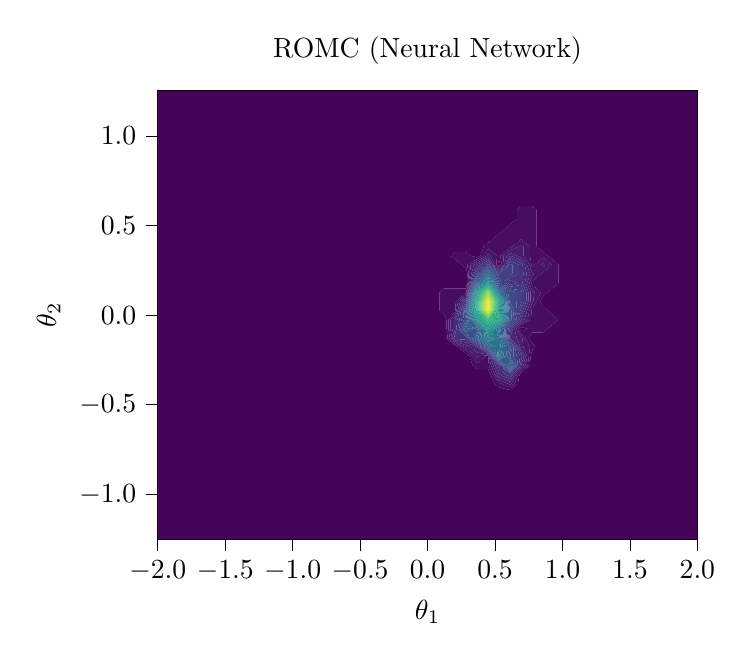
\begin{tikzpicture}

\definecolor{color0}{rgb}{0.269944,0.014625,0.341379}
\definecolor{color1}{rgb}{0.277018,0.050344,0.375715}
\definecolor{color2}{rgb}{0.281446,0.08432,0.407414}
\definecolor{color3}{rgb}{0.283197,0.11568,0.436115}
\definecolor{color4}{rgb}{0.28229,0.145912,0.46151}
\definecolor{color5}{rgb}{0.278826,0.17549,0.483397}
\definecolor{color6}{rgb}{0.274128,0.199721,0.498911}
\definecolor{color7}{rgb}{0.26658,0.228262,0.514349}
\definecolor{color8}{rgb}{0.257322,0.25613,0.526563}
\definecolor{color9}{rgb}{0.246811,0.283237,0.535941}
\definecolor{color10}{rgb}{0.235526,0.309527,0.542944}
\definecolor{color11}{rgb}{0.225863,0.330805,0.547314}
\definecolor{color12}{rgb}{0.214298,0.355619,0.551184}
\definecolor{color13}{rgb}{0.203063,0.379716,0.553925}
\definecolor{color14}{rgb}{0.192357,0.403199,0.555836}
\definecolor{color15}{rgb}{0.182256,0.426184,0.55712}
\definecolor{color16}{rgb}{0.172719,0.448791,0.557885}
\definecolor{color17}{rgb}{0.165117,0.467423,0.558141}
\definecolor{color18}{rgb}{0.15627,0.489624,0.557936}
\definecolor{color19}{rgb}{0.147607,0.511733,0.557049}
\definecolor{color20}{rgb}{0.139147,0.533812,0.555298}
\definecolor{color21}{rgb}{0.131172,0.555899,0.552459}
\definecolor{color22}{rgb}{0.125394,0.574318,0.549086}
\definecolor{color23}{rgb}{0.120565,0.596422,0.543611}
\definecolor{color24}{rgb}{0.119699,0.61849,0.536347}
\definecolor{color25}{rgb}{0.12478,0.640461,0.527068}
\definecolor{color26}{rgb}{0.137339,0.662252,0.515571}
\definecolor{color27}{rgb}{0.157851,0.683765,0.501686}
\definecolor{color28}{rgb}{0.180653,0.701402,0.488189}
\definecolor{color29}{rgb}{0.214,0.722114,0.469588}
\definecolor{color30}{rgb}{0.252899,0.742211,0.448284}
\definecolor{color31}{rgb}{0.296479,0.761561,0.424223}
\definecolor{color32}{rgb}{0.344074,0.780029,0.397381}
\definecolor{color33}{rgb}{0.386433,0.794644,0.372886}
\definecolor{color34}{rgb}{0.440137,0.811138,0.340967}
\definecolor{color35}{rgb}{0.496615,0.826376,0.306377}
\definecolor{color36}{rgb}{0.555484,0.840254,0.269281}
\definecolor{color37}{rgb}{0.616293,0.852709,0.230052}
\definecolor{color38}{rgb}{0.668054,0.861999,0.196293}
\definecolor{color39}{rgb}{0.730889,0.871916,0.156029}
\definecolor{color40}{rgb}{0.79376,0.880678,0.120005}
\definecolor{color41}{rgb}{0.85581,0.888601,0.097452}
\definecolor{color42}{rgb}{0.916242,0.896091,0.100717}
\definecolor{color43}{rgb}{0.974417,0.90359,0.130215}

\begin{axis}[
tick align=outside,
tick pos=left,
title={ROMC (Neural Network)},
x grid style={white!69.0196078431373!black},
xlabel={\(\displaystyle \theta_1\)},
xmin=-2, xmax=2,
xtick style={color=black},
xtick={-2,-1.5,-1,-0.5,0,0.5,1,1.5,2},
xticklabels={
  \(\displaystyle {\ensuremath{-}2.0}\),
  \(\displaystyle {\ensuremath{-}1.5}\),
  \(\displaystyle {\ensuremath{-}1.0}\),
  \(\displaystyle {\ensuremath{-}0.5}\),
  \(\displaystyle {0.0}\),
  \(\displaystyle {0.5}\),
  \(\displaystyle {1.0}\),
  \(\displaystyle {1.5}\),
  \(\displaystyle {2.0}\)
},
y grid style={white!69.0196078431373!black},
ylabel={\(\displaystyle \theta_2\)},
ymin=-1.25, ymax=1.25,
ytick style={color=black},
ytick={-1.5,-1,-0.5,0,0.5,1,1.5},
yticklabels={
  \(\displaystyle {\ensuremath{-}1.5}\),
  \(\displaystyle {\ensuremath{-}1.0}\),
  \(\displaystyle {\ensuremath{-}0.5}\),
  \(\displaystyle {0.0}\),
  \(\displaystyle {0.5}\),
  \(\displaystyle {1.0}\),
  \(\displaystyle {1.5}\)
}
]
\addplot [draw=none, fill=color0]
table{%
x  y
-1.91836734693878 -1.25
-1.83673469387755 -1.25
-1.75510204081633 -1.25
-1.6734693877551 -1.25
-1.59183673469388 -1.25
-1.51020408163265 -1.25
-1.42857142857143 -1.25
-1.3469387755102 -1.25
-1.26530612244898 -1.25
-1.18367346938776 -1.25
-1.10204081632653 -1.25
-1.02040816326531 -1.25
-0.938775510204082 -1.25
-0.857142857142857 -1.25
-0.775510204081633 -1.25
-0.693877551020408 -1.25
-0.612244897959184 -1.25
-0.530612244897959 -1.25
-0.448979591836735 -1.25
-0.36734693877551 -1.25
-0.285714285714286 -1.25
-0.204081632653061 -1.25
-0.122448979591837 -1.25
-0.0408163265306123 -1.25
0.0408163265306123 -1.25
0.122448979591836 -1.25
0.204081632653061 -1.25
0.285714285714286 -1.25
0.36734693877551 -1.25
0.448979591836734 -1.25
0.530612244897959 -1.25
0.612244897959183 -1.25
0.693877551020408 -1.25
0.775510204081633 -1.25
0.857142857142857 -1.25
0.938775510204081 -1.25
1.02040816326531 -1.25
1.10204081632653 -1.25
1.18367346938775 -1.25
1.26530612244898 -1.25
1.3469387755102 -1.25
1.42857142857143 -1.25
1.51020408163265 -1.25
1.59183673469388 -1.25
1.6734693877551 -1.25
1.75510204081633 -1.25
1.83673469387755 -1.25
1.91836734693878 -1.25
2 -1.25
2 -1.19897959183673
2 -1.14795918367347
2 -1.0969387755102
2 -1.04591836734694
2 -0.994897959183674
2 -0.943877551020408
2 -0.892857142857143
2 -0.841836734693878
2 -0.790816326530612
2 -0.739795918367347
2 -0.688775510204082
2 -0.637755102040816
2 -0.586734693877551
2 -0.535714285714286
2 -0.48469387755102
2 -0.433673469387755
2 -0.38265306122449
2 -0.331632653061224
2 -0.280612244897959
2 -0.229591836734694
2 -0.178571428571429
2 -0.127551020408163
2 -0.0765306122448979
2 -0.0255102040816326
2 0.0255102040816326
2 0.0765306122448979
2 0.127551020408163
2 0.178571428571429
2 0.229591836734694
2 0.280612244897959
2 0.331632653061225
2 0.38265306122449
2 0.433673469387755
2 0.48469387755102
2 0.535714285714286
2 0.586734693877551
2 0.637755102040816
2 0.688775510204082
2 0.739795918367347
2 0.790816326530612
2 0.841836734693878
2 0.892857142857143
2 0.943877551020408
2 0.994897959183674
2 1.04591836734694
2 1.0969387755102
2 1.14795918367347
2 1.19897959183673
2 1.25
1.91836734693878 1.25
1.83673469387755 1.25
1.75510204081633 1.25
1.6734693877551 1.25
1.59183673469388 1.25
1.51020408163265 1.25
1.42857142857143 1.25
1.3469387755102 1.25
1.26530612244898 1.25
1.18367346938775 1.25
1.10204081632653 1.25
1.02040816326531 1.25
0.938775510204081 1.25
0.857142857142857 1.25
0.775510204081633 1.25
0.693877551020408 1.25
0.612244897959183 1.25
0.530612244897959 1.25
0.448979591836734 1.25
0.36734693877551 1.25
0.285714285714286 1.25
0.204081632653061 1.25
0.122448979591836 1.25
0.0408163265306123 1.25
-0.0408163265306123 1.25
-0.122448979591837 1.25
-0.204081632653061 1.25
-0.285714285714286 1.25
-0.36734693877551 1.25
-0.448979591836735 1.25
-0.530612244897959 1.25
-0.612244897959184 1.25
-0.693877551020408 1.25
-0.775510204081633 1.25
-0.857142857142857 1.25
-0.938775510204082 1.25
-1.02040816326531 1.25
-1.10204081632653 1.25
-1.18367346938776 1.25
-1.26530612244898 1.25
-1.3469387755102 1.25
-1.42857142857143 1.25
-1.51020408163265 1.25
-1.59183673469388 1.25
-1.6734693877551 1.25
-1.75510204081633 1.25
-1.83673469387755 1.25
-1.91836734693878 1.25
-2 1.25
-2 1.19897959183673
-2 1.14795918367347
-2 1.0969387755102
-2 1.04591836734694
-2 0.994897959183674
-2 0.943877551020408
-2 0.892857142857143
-2 0.841836734693878
-2 0.790816326530612
-2 0.739795918367347
-2 0.688775510204082
-2 0.637755102040816
-2 0.586734693877551
-2 0.535714285714286
-2 0.48469387755102
-2 0.433673469387755
-2 0.38265306122449
-2 0.331632653061225
-2 0.280612244897959
-2 0.229591836734694
-2 0.178571428571429
-2 0.127551020408163
-2 0.0765306122448979
-2 0.0255102040816326
-2 -0.0255102040816326
-2 -0.0765306122448979
-2 -0.127551020408163
-2 -0.178571428571429
-2 -0.229591836734694
-2 -0.280612244897959
-2 -0.331632653061224
-2 -0.38265306122449
-2 -0.433673469387755
-2 -0.48469387755102
-2 -0.535714285714286
-2 -0.586734693877551
-2 -0.637755102040816
-2 -0.688775510204082
-2 -0.739795918367347
-2 -0.790816326530612
-2 -0.841836734693878
-2 -0.892857142857143
-2 -0.943877551020408
-2 -0.994897959183674
-2 -1.04591836734694
-2 -1.0969387755102
-2 -1.14795918367347
-2 -1.19897959183673
-2 -1.25
-1.91836734693878 -1.25

0.497959183673469 -0.38265306122449
0.465306122448979 -0.331632653061224
0.448979591836734 -0.301020408163265
0.36734693877551 -0.301020408163265
0.33469387755102 -0.280612244897959
0.310204081632653 -0.229591836734694
0.285714285714286 -0.214285714285714
0.228571428571428 -0.178571428571429
0.204081632653061 -0.170918367346939
0.13469387755102 -0.127551020408163
0.138775510204081 -0.0765306122448979
0.138775510204081 -0.0255102040816326
0.122448979591836 0.00510204081632653
0.0897959183673468 0.0255102040816326
0.0897959183673468 0.0765306122448979
0.0897959183673468 0.127551020408163
0.122448979591836 0.147959183673469
0.204081632653061 0.147959183673469
0.285714285714286 0.147959183673469
0.291836734693877 0.178571428571429
0.295510204081633 0.229591836734694
0.285714285714286 0.260204081632653
0.253061224489796 0.280612244897959
0.204081632653061 0.311224489795918
0.171428571428571 0.331632653061225
0.204081632653061 0.352040816326531
0.285714285714286 0.352040816326531
0.318367346938775 0.331632653061225
0.36734693877551 0.321428571428572
0.391836734693877 0.331632653061225
0.416326530612245 0.38265306122449
0.448979591836734 0.403061224489796
0.497959183673469 0.433673469387755
0.530612244897959 0.454081632653061
0.579591836734694 0.48469387755102
0.612244897959183 0.505102040816326
0.661224489795918 0.535714285714286
0.661224489795918 0.586734693877551
0.693877551020408 0.607142857142857
0.775510204081633 0.607142857142857
0.808163265306122 0.586734693877551
0.808163265306122 0.535714285714286
0.808163265306122 0.48469387755102
0.808163265306122 0.433673469387755
0.808163265306122 0.38265306122449
0.857142857142857 0.352040816326531
0.889795918367347 0.331632653061225
0.938775510204081 0.301020408163265
0.971428571428571 0.280612244897959
0.971428571428571 0.229591836734694
0.971428571428571 0.178571428571429
0.938775510204081 0.158163265306123
0.889795918367347 0.127551020408163
0.857142857142857 0.107142857142857
0.832653061224489 0.0765306122448979
0.857142857142857 0.0459183673469387
0.889795918367347 0.0255102040816326
0.938775510204081 -0.00510204081632653
0.971428571428571 -0.0255102040816326
0.938775510204081 -0.0459183673469387
0.889795918367347 -0.0765306122448979
0.857142857142857 -0.096938775510204
0.775510204081633 -0.096938775510204
0.751020408163265 -0.127551020408163
0.775510204081633 -0.158163265306122
0.808163265306122 -0.178571428571429
0.775510204081633 -0.198979591836735
0.763265306122449 -0.229591836734694
0.759183673469388 -0.280612244897959
0.693877551020408 -0.321428571428571
0.681632653061224 -0.331632653061224
0.669387755102041 -0.38265306122449
0.612244897959183 -0.418367346938776
0.530612244897959 -0.403061224489796
0.497959183673469 -0.38265306122449
};
\addplot [draw=none, fill=color0]
table{%
x  y
0.693877551020408 -0.0918367346938775
0.742857142857143 -0.0765306122448979
0.693877551020408 -0.0663265306122448
0.681632653061224 -0.0765306122448979
0.693877551020408 -0.0918367346938775
};
\addplot [draw=none, fill=color0]
table{%
x  y
0.530612244897959 0.274489795918367
0.540408163265306 0.280612244897959
0.530612244897959 0.311224489795918
0.520816326530612 0.280612244897959
0.530612244897959 0.274489795918367
};
\addplot [draw=none, fill=color1]
table{%
x  y
0.530612244897959 -0.403061224489796
0.612244897959183 -0.418367346938776
0.669387755102041 -0.38265306122449
0.681632653061224 -0.331632653061224
0.693877551020408 -0.321428571428571
0.759183673469388 -0.280612244897959
0.763265306122449 -0.229591836734694
0.775510204081633 -0.198979591836735
0.808163265306122 -0.178571428571429
0.775510204081633 -0.158163265306122
0.751020408163265 -0.127551020408163
0.775510204081633 -0.096938775510204
0.857142857142857 -0.096938775510204
0.889795918367347 -0.0765306122448979
0.938775510204081 -0.0459183673469387
0.971428571428571 -0.0255102040816326
0.938775510204081 -0.00510204081632653
0.889795918367347 0.0255102040816326
0.857142857142857 0.0459183673469387
0.832653061224489 0.0765306122448979
0.857142857142857 0.107142857142857
0.889795918367347 0.127551020408163
0.938775510204081 0.158163265306123
0.971428571428571 0.178571428571429
0.971428571428571 0.229591836734694
0.971428571428571 0.280612244897959
0.938775510204081 0.301020408163265
0.889795918367347 0.331632653061225
0.857142857142857 0.352040816326531
0.808163265306122 0.38265306122449
0.808163265306122 0.433673469387755
0.808163265306122 0.48469387755102
0.808163265306122 0.535714285714286
0.808163265306122 0.586734693877551
0.775510204081633 0.607142857142857
0.693877551020408 0.607142857142857
0.661224489795918 0.586734693877551
0.661224489795918 0.535714285714286
0.612244897959183 0.505102040816326
0.579591836734694 0.48469387755102
0.530612244897959 0.454081632653061
0.497959183673469 0.433673469387755
0.448979591836734 0.403061224489796
0.416326530612245 0.38265306122449
0.391836734693877 0.331632653061225
0.36734693877551 0.321428571428572
0.318367346938775 0.331632653061225
0.285714285714286 0.352040816326531
0.204081632653061 0.352040816326531
0.171428571428571 0.331632653061225
0.204081632653061 0.311224489795918
0.253061224489796 0.280612244897959
0.285714285714286 0.260204081632653
0.295510204081633 0.229591836734694
0.291836734693877 0.178571428571429
0.285714285714286 0.147959183673469
0.204081632653061 0.147959183673469
0.122448979591836 0.147959183673469
0.0897959183673468 0.127551020408163
0.0897959183673468 0.0765306122448979
0.0897959183673468 0.0255102040816326
0.122448979591836 0.00510204081632653
0.138775510204081 -0.0255102040816326
0.138775510204081 -0.0765306122448979
0.13469387755102 -0.127551020408163
0.204081632653061 -0.170918367346939
0.228571428571428 -0.178571428571429
0.285714285714286 -0.214285714285714
0.310204081632653 -0.229591836734694
0.33469387755102 -0.280612244897959
0.36734693877551 -0.301020408163265
0.448979591836734 -0.301020408163265
0.465306122448979 -0.331632653061224
0.497959183673469 -0.38265306122449
0.530612244897959 -0.403061224489796

0.546938775510204 -0.38265306122449
0.530612244897959 -0.377551020408163
0.481632653061224 -0.331632653061224
0.454421768707483 -0.280612244897959
0.450612244897959 -0.229591836734694
0.448979591836734 -0.228134110787172
0.432653061224489 -0.229591836734694
0.36734693877551 -0.270408163265306
0.33469387755102 -0.229591836734694
0.285714285714286 -0.198979591836735
0.253061224489796 -0.178571428571429
0.204081632653061 -0.163265306122449
0.146938775510204 -0.127551020408163
0.155102040816326 -0.0765306122448979
0.155102040816326 -0.0255102040816326
0.204081632653061 0.0204081632653061
0.206802721088435 0.0255102040816326
0.209523809523809 0.0765306122448979
0.285714285714286 0.124149659863946
0.286970172684458 0.127551020408163
0.297959183673469 0.178571428571429
0.305306122448979 0.229591836734694
0.293877551020408 0.280612244897959
0.36734693877551 0.311224489795918
0.416326530612245 0.331632653061225
0.448979591836734 0.372448979591837
0.514285714285714 0.331632653061225
0.511020408163265 0.280612244897959
0.530612244897959 0.268367346938776
0.550204081632653 0.280612244897959
0.538775510204081 0.331632653061225
0.612244897959183 0.377551020408163
0.628571428571428 0.38265306122449
0.693877551020408 0.423469387755102
0.759183673469388 0.38265306122449
0.759183673469388 0.331632653061225
0.770068027210884 0.280612244897959
0.775510204081633 0.270408163265306
0.791836734693877 0.280612244897959
0.857142857142857 0.321428571428572
0.922448979591836 0.280612244897959
0.857142857142857 0.239795918367347
0.840816326530612 0.229591836734694
0.775510204081633 0.188775510204082
0.770068027210884 0.178571428571429
0.775510204081633 0.168367346938776
0.840816326530612 0.127551020408163
0.808163265306122 0.0765306122448979
0.775510204081633 0.0357142857142857
0.770068027210884 0.0255102040816326
0.76734693877551 -0.0255102040816326
0.693877551020408 -0.0561224489795918
0.669387755102041 -0.0765306122448979
0.693877551020408 -0.107142857142857
0.726530612244898 -0.127551020408163
0.759183673469388 -0.178571428571429
0.751020408163265 -0.229591836734694
0.742857142857143 -0.280612244897959
0.693877551020408 -0.311224489795918
0.669387755102041 -0.331632653061224
0.644897959183673 -0.38265306122449
0.612244897959183 -0.403061224489796
0.546938775510204 -0.38265306122449

0.681632653061224 -0.0765306122448979
0.693877551020408 -0.0663265306122448
0.742857142857143 -0.0765306122448979
0.693877551020408 -0.0918367346938775
0.681632653061224 -0.0765306122448979

0.520816326530612 0.280612244897959
0.530612244897959 0.311224489795918
0.540408163265306 0.280612244897959
0.530612244897959 0.274489795918367
0.520816326530612 0.280612244897959
};
\addplot [draw=none, fill=color2]
table{%
x  y
0.612244897959183 -0.403061224489796
0.644897959183673 -0.38265306122449
0.669387755102041 -0.331632653061224
0.693877551020408 -0.311224489795918
0.742857142857143 -0.280612244897959
0.751020408163265 -0.229591836734694
0.759183673469388 -0.178571428571429
0.726530612244898 -0.127551020408163
0.693877551020408 -0.107142857142857
0.669387755102041 -0.0765306122448979
0.693877551020408 -0.0561224489795918
0.76734693877551 -0.0255102040816326
0.770068027210884 0.0255102040816326
0.775510204081633 0.0357142857142857
0.808163265306122 0.0765306122448979
0.840816326530612 0.127551020408163
0.775510204081633 0.168367346938776
0.770068027210884 0.178571428571429
0.775510204081633 0.188775510204082
0.840816326530612 0.229591836734694
0.857142857142857 0.239795918367347
0.922448979591836 0.280612244897959
0.857142857142857 0.321428571428572
0.791836734693877 0.280612244897959
0.775510204081633 0.270408163265306
0.770068027210884 0.280612244897959
0.759183673469388 0.331632653061225
0.759183673469388 0.38265306122449
0.693877551020408 0.423469387755102
0.628571428571428 0.38265306122449
0.612244897959183 0.377551020408163
0.538775510204081 0.331632653061225
0.550204081632653 0.280612244897959
0.530612244897959 0.268367346938776
0.511020408163265 0.280612244897959
0.514285714285714 0.331632653061225
0.448979591836734 0.372448979591837
0.416326530612245 0.331632653061225
0.36734693877551 0.311224489795918
0.293877551020408 0.280612244897959
0.305306122448979 0.229591836734694
0.297959183673469 0.178571428571429
0.286970172684458 0.127551020408163
0.285714285714286 0.124149659863946
0.209523809523809 0.0765306122448979
0.206802721088435 0.0255102040816326
0.204081632653061 0.0204081632653061
0.155102040816326 -0.0255102040816326
0.155102040816326 -0.0765306122448979
0.146938775510204 -0.127551020408163
0.204081632653061 -0.163265306122449
0.253061224489796 -0.178571428571429
0.285714285714286 -0.198979591836735
0.33469387755102 -0.229591836734694
0.36734693877551 -0.270408163265306
0.432653061224489 -0.229591836734694
0.448979591836734 -0.228134110787172
0.450612244897959 -0.229591836734694
0.454421768707483 -0.280612244897959
0.481632653061224 -0.331632653061224
0.530612244897959 -0.377551020408163
0.546938775510204 -0.38265306122449
0.612244897959183 -0.403061224489796

0.595918367346939 -0.38265306122449
0.530612244897959 -0.362244897959184
0.497959183673469 -0.331632653061224
0.470748299319728 -0.280612244897959
0.455510204081632 -0.229591836734694
0.448979591836734 -0.223760932944606
0.383673469387755 -0.229591836734694
0.36734693877551 -0.239795918367347
0.359183673469388 -0.229591836734694
0.285714285714286 -0.183673469387755
0.277551020408163 -0.178571428571429
0.204081632653061 -0.155612244897959
0.159183673469387 -0.127551020408163
0.171428571428571 -0.0765306122448979
0.171428571428571 -0.0255102040816326
0.204081632653061 0.00510204081632652
0.214965986394558 0.0255102040816326
0.225850340136054 0.0765306122448979
0.285714285714286 0.113945578231293
0.290737833594976 0.127551020408163
0.304081632653061 0.178571428571429
0.315102040816326 0.229591836734694
0.318367346938775 0.280612244897959
0.36734693877551 0.301020408163265
0.440816326530612 0.331632653061225
0.448979591836734 0.341836734693878
0.465306122448979 0.331632653061225
0.501224489795918 0.280612244897959
0.530612244897959 0.262244897959184
0.56 0.280612244897959
0.563265306122449 0.331632653061225
0.612244897959183 0.362244897959184
0.677551020408163 0.38265306122449
0.693877551020408 0.392857142857143
0.710204081632653 0.38265306122449
0.710204081632653 0.331632653061225
0.753741496598639 0.280612244897959
0.775510204081633 0.239795918367347
0.791836734693877 0.229591836734694
0.775510204081633 0.219387755102041
0.753741496598639 0.178571428571429
0.775510204081633 0.137755102040816
0.791836734693877 0.127551020408163
0.783673469387755 0.0765306122448979
0.775510204081633 0.0663265306122448
0.753741496598639 0.0255102040816326
0.742857142857143 -0.0255102040816326
0.693877551020408 -0.0459183673469387
0.657142857142857 -0.0765306122448979
0.693877551020408 -0.122448979591837
0.70204081632653 -0.127551020408163
0.710204081632653 -0.178571428571429
0.738775510204082 -0.229591836734694
0.726530612244898 -0.280612244897959
0.693877551020408 -0.301020408163265
0.657142857142857 -0.331632653061224
0.620408163265306 -0.38265306122449
0.612244897959183 -0.387755102040816
0.595918367346939 -0.38265306122449

0.840816326530612 0.280612244897959
0.857142857142857 0.290816326530612
0.873469387755102 0.280612244897959
0.857142857142857 0.270408163265306
0.840816326530612 0.280612244897959
};
\addplot [draw=none, fill=color3]
table{%
x  y
0.612244897959183 -0.387755102040816
0.620408163265306 -0.38265306122449
0.657142857142857 -0.331632653061224
0.693877551020408 -0.301020408163265
0.726530612244898 -0.280612244897959
0.738775510204082 -0.229591836734694
0.710204081632653 -0.178571428571429
0.70204081632653 -0.127551020408163
0.693877551020408 -0.122448979591837
0.657142857142857 -0.0765306122448979
0.693877551020408 -0.0459183673469387
0.742857142857143 -0.0255102040816326
0.753741496598639 0.0255102040816326
0.775510204081633 0.0663265306122448
0.783673469387755 0.0765306122448979
0.791836734693877 0.127551020408163
0.775510204081633 0.137755102040816
0.753741496598639 0.178571428571429
0.775510204081633 0.219387755102041
0.791836734693877 0.229591836734694
0.775510204081633 0.239795918367347
0.753741496598639 0.280612244897959
0.710204081632653 0.331632653061225
0.710204081632653 0.38265306122449
0.693877551020408 0.392857142857143
0.677551020408163 0.38265306122449
0.612244897959183 0.362244897959184
0.563265306122449 0.331632653061225
0.56 0.280612244897959
0.530612244897959 0.262244897959184
0.501224489795918 0.280612244897959
0.465306122448979 0.331632653061225
0.448979591836734 0.341836734693878
0.440816326530612 0.331632653061225
0.36734693877551 0.301020408163265
0.318367346938775 0.280612244897959
0.315102040816326 0.229591836734694
0.304081632653061 0.178571428571429
0.290737833594976 0.127551020408163
0.285714285714286 0.113945578231293
0.225850340136054 0.0765306122448979
0.214965986394558 0.0255102040816326
0.204081632653061 0.00510204081632652
0.171428571428571 -0.0255102040816326
0.171428571428571 -0.0765306122448979
0.159183673469387 -0.127551020408163
0.204081632653061 -0.155612244897959
0.277551020408163 -0.178571428571429
0.285714285714286 -0.183673469387755
0.359183673469388 -0.229591836734694
0.36734693877551 -0.239795918367347
0.383673469387755 -0.229591836734694
0.448979591836734 -0.223760932944606
0.455510204081632 -0.229591836734694
0.470748299319728 -0.280612244897959
0.497959183673469 -0.331632653061224
0.530612244897959 -0.362244897959184
0.595918367346939 -0.38265306122449
0.612244897959183 -0.387755102040816

0.514285714285714 -0.331632653061224
0.487074829931972 -0.280612244897959
0.460408163265306 -0.229591836734694
0.448979591836734 -0.219387755102041
0.36734693877551 -0.209183673469388
0.318367346938775 -0.178571428571429
0.285714285714286 -0.168367346938776
0.204081632653061 -0.147959183673469
0.171428571428571 -0.127551020408163
0.187755102040816 -0.0765306122448979
0.187755102040816 -0.0255102040816326
0.204081632653061 -0.0102040816326531
0.22312925170068 0.0255102040816326
0.242176870748299 0.0765306122448979
0.285714285714286 0.103741496598639
0.294505494505494 0.127551020408163
0.310204081632653 0.178571428571429
0.324897959183673 0.229591836734694
0.342857142857143 0.280612244897959
0.36734693877551 0.290816326530612
0.448979591836734 0.324829931972789
0.491428571428571 0.280612244897959
0.530612244897959 0.256122448979592
0.569795918367347 0.280612244897959
0.587755102040816 0.331632653061225
0.612244897959183 0.346938775510204
0.661224489795918 0.331632653061225
0.693877551020408 0.321428571428572
0.737414965986394 0.280612244897959
0.759183673469388 0.229591836734694
0.737414965986394 0.178571428571429
0.764625850340136 0.127551020408163
0.764625850340136 0.0765306122448979
0.737414965986394 0.0255102040816326
0.718367346938775 -0.0255102040816326
0.693877551020408 -0.0357142857142857
0.644897959183673 -0.0765306122448979
0.661224489795918 -0.127551020408163
0.68734693877551 -0.178571428571429
0.693877551020408 -0.188775510204082
0.726530612244898 -0.229591836734694
0.710204081632653 -0.280612244897959
0.693877551020408 -0.290816326530612
0.644897959183673 -0.331632653061224
0.612244897959183 -0.372448979591837
0.530612244897959 -0.346938775510204
0.514285714285714 -0.331632653061224
};
\addplot [draw=none, fill=color3]
table{%
x  y
0.857142857142857 0.270408163265306
0.873469387755102 0.280612244897959
0.857142857142857 0.290816326530612
0.840816326530612 0.280612244897959
0.857142857142857 0.270408163265306
};
\addplot [draw=none, fill=color4]
table{%
x  y
0.530612244897959 -0.346938775510204
0.612244897959183 -0.372448979591837
0.644897959183673 -0.331632653061224
0.693877551020408 -0.290816326530612
0.710204081632653 -0.280612244897959
0.726530612244898 -0.229591836734694
0.693877551020408 -0.188775510204082
0.68734693877551 -0.178571428571429
0.661224489795918 -0.127551020408163
0.644897959183673 -0.0765306122448979
0.693877551020408 -0.0357142857142857
0.718367346938775 -0.0255102040816326
0.737414965986394 0.0255102040816326
0.764625850340136 0.0765306122448979
0.764625850340136 0.127551020408163
0.737414965986394 0.178571428571429
0.759183673469388 0.229591836734694
0.737414965986394 0.280612244897959
0.693877551020408 0.321428571428572
0.661224489795918 0.331632653061225
0.612244897959183 0.346938775510204
0.587755102040816 0.331632653061225
0.569795918367347 0.280612244897959
0.530612244897959 0.256122448979592
0.491428571428571 0.280612244897959
0.448979591836734 0.324829931972789
0.36734693877551 0.290816326530612
0.342857142857143 0.280612244897959
0.324897959183673 0.229591836734694
0.310204081632653 0.178571428571429
0.294505494505494 0.127551020408163
0.285714285714286 0.103741496598639
0.242176870748299 0.0765306122448979
0.22312925170068 0.0255102040816326
0.204081632653061 -0.0102040816326531
0.187755102040816 -0.0255102040816326
0.187755102040816 -0.0765306122448979
0.171428571428571 -0.127551020408163
0.204081632653061 -0.147959183673469
0.285714285714286 -0.168367346938776
0.318367346938775 -0.178571428571429
0.36734693877551 -0.209183673469388
0.448979591836734 -0.219387755102041
0.460408163265306 -0.229591836734694
0.487074829931972 -0.280612244897959
0.514285714285714 -0.331632653061224
0.530612244897959 -0.346938775510204

0.530612244897959 -0.331632653061224
0.530612244897959 -0.331632653061224
0.503401360544217 -0.280612244897959
0.465306122448979 -0.229591836734694
0.448979591836734 -0.215014577259475
0.36734693877551 -0.178571428571429
0.285714285714286 -0.153061224489796
0.204081632653061 -0.140306122448979
0.183673469387755 -0.127551020408163
0.204081632653061 -0.0765306122448979
0.204081632653061 -0.0765306122448979
0.204081632653061 -0.0255102040816326
0.231292517006803 0.0255102040816326
0.258503401360544 0.0765306122448979
0.285714285714286 0.0935374149659864
0.298273155416012 0.127551020408163
0.316326530612245 0.178571428571429
0.33469387755102 0.229591836734694
0.36734693877551 0.280612244897959
0.36734693877551 0.280612244897959
0.448979591836734 0.314625850340136
0.481632653061224 0.280612244897959
0.530612244897959 0.25
0.579591836734694 0.280612244897959
0.612244897959183 0.331632653061225
0.693877551020408 0.306122448979592
0.72108843537415 0.280612244897959
0.73469387755102 0.229591836734694
0.72108843537415 0.178571428571429
0.748299319727891 0.127551020408163
0.748299319727891 0.0765306122448979
0.72108843537415 0.0255102040816326
0.693877551020408 -0.0255102040816326
0.693877551020408 -0.0255102040816326
0.63265306122449 -0.0765306122448979
0.612244897959183 -0.127551020408163
0.612244897959183 -0.127551020408163
0.612244897959183 -0.127551020408163
0.677551020408163 -0.178571428571429
0.693877551020408 -0.204081632653061
0.714285714285714 -0.229591836734694
0.693877551020408 -0.280612244897959
0.693877551020408 -0.280612244897959
0.63265306122449 -0.331632653061224
0.612244897959183 -0.357142857142857
0.530612244897959 -0.331632653061224
};
\addplot [draw=none, fill=color4]
table{%
x  y
0.612244897959183 0.178571428571429
0.612244897959184 0.178571428571429
0.612244897959183 0.178571428571429
0.612244897959183 0.178571428571429
0.612244897959183 0.178571428571429
};
\addplot [draw=none, fill=color5]
table{%
x  y
0.612244897959183 -0.357142857142857
0.63265306122449 -0.331632653061224
0.693877551020408 -0.280612244897959
0.714285714285714 -0.229591836734694
0.693877551020408 -0.204081632653061
0.677551020408163 -0.178571428571429
0.612244897959183 -0.127551020408163
0.612244897959183 -0.127551020408163
0.63265306122449 -0.0765306122448979
0.693877551020408 -0.0255102040816326
0.693877551020408 -0.0255102040816326
0.72108843537415 0.0255102040816326
0.748299319727891 0.0765306122448979
0.748299319727891 0.127551020408163
0.72108843537415 0.178571428571429
0.73469387755102 0.229591836734694
0.72108843537415 0.280612244897959
0.693877551020408 0.306122448979592
0.612244897959183 0.331632653061225
0.579591836734694 0.280612244897959
0.530612244897959 0.25
0.481632653061224 0.280612244897959
0.448979591836734 0.314625850340136
0.36734693877551 0.280612244897959
0.36734693877551 0.280612244897959
0.33469387755102 0.229591836734694
0.316326530612245 0.178571428571429
0.298273155416012 0.127551020408163
0.285714285714286 0.0935374149659864
0.258503401360544 0.0765306122448979
0.231292517006803 0.0255102040816326
0.204081632653061 -0.0255102040816326
0.204081632653061 -0.0765306122448979
0.204081632653061 -0.0765306122448979
0.183673469387755 -0.127551020408163
0.204081632653061 -0.140306122448979
0.285714285714286 -0.153061224489796
0.36734693877551 -0.178571428571429
0.36734693877551 -0.178571428571429
0.448979591836734 -0.215014577259475
0.465306122448979 -0.229591836734694
0.503401360544217 -0.280612244897959
0.530612244897959 -0.331632653061224
0.530612244897959 -0.331632653061224
0.612244897959183 -0.357142857142857

0.579591836734694 -0.331632653061224
0.530612244897959 -0.301020408163265
0.519727891156462 -0.280612244897959
0.470204081632653 -0.229591836734694
0.448979591836734 -0.21064139941691
0.377142857142857 -0.178571428571429
0.36734693877551 -0.172448979591837
0.285714285714286 -0.137755102040816
0.204081632653061 -0.13265306122449
0.195918367346939 -0.127551020408163
0.204081632653061 -0.107142857142857
0.213877551020408 -0.0765306122448979
0.220408163265306 -0.0255102040816326
0.239455782312925 0.0255102040816326
0.274829931972789 0.0765306122448979
0.285714285714286 0.0833333333333333
0.302040816326531 0.127551020408163
0.322448979591837 0.178571428571429
0.344489795918367 0.229591836734694
0.36734693877551 0.26530612244898
0.391836734693877 0.280612244897959
0.448979591836734 0.304421768707483
0.471836734693877 0.280612244897959
0.530612244897959 0.243877551020408
0.589387755102041 0.280612244897959
0.612244897959183 0.316326530612245
0.693877551020408 0.290816326530612
0.704761904761905 0.280612244897959
0.710204081632653 0.229591836734694
0.704761904761905 0.178571428571429
0.731972789115646 0.127551020408163
0.731972789115646 0.0765306122448979
0.704761904761905 0.0255102040816326
0.693877551020408 0.00510204081632655
0.681632653061224 -0.0255102040816326
0.620408163265306 -0.0765306122448979
0.612244897959183 -0.0969387755102039
0.605247813411079 -0.127551020408163
0.612244897959183 -0.135204081632653
0.667755102040816 -0.178571428571429
0.693877551020408 -0.219387755102041
0.70204081632653 -0.229591836734694
0.693877551020408 -0.25
0.685714285714286 -0.280612244897959
0.620408163265306 -0.331632653061224
0.612244897959183 -0.341836734693878
0.579591836734694 -0.331632653061224
};
\addplot [draw=none, fill=color5]
table{%
x  y
0.612244897959183 0.168367346938776
0.661224489795918 0.178571428571429
0.612244897959183 0.193877551020408
0.595918367346938 0.178571428571429
0.612244897959183 0.168367346938776

0.612244897959183 0.178571428571429
0.612244897959183 0.178571428571429
0.612244897959184 0.178571428571429
0.612244897959183 0.178571428571429
0.612244897959183 0.178571428571429
};
\addplot [draw=none, fill=color6]
table{%
x  y
0.612244897959183 -0.341836734693878
0.620408163265306 -0.331632653061224
0.685714285714286 -0.280612244897959
0.693877551020408 -0.25
0.70204081632653 -0.229591836734694
0.693877551020408 -0.219387755102041
0.667755102040816 -0.178571428571429
0.612244897959183 -0.135204081632653
0.605247813411078 -0.127551020408163
0.612244897959183 -0.0969387755102039
0.620408163265306 -0.0765306122448979
0.681632653061224 -0.0255102040816326
0.693877551020408 0.00510204081632655
0.704761904761905 0.0255102040816326
0.731972789115646 0.0765306122448979
0.731972789115646 0.127551020408163
0.704761904761905 0.178571428571429
0.710204081632653 0.229591836734694
0.704761904761905 0.280612244897959
0.693877551020408 0.290816326530612
0.612244897959183 0.316326530612245
0.589387755102041 0.280612244897959
0.530612244897959 0.243877551020408
0.471836734693877 0.280612244897959
0.448979591836734 0.304421768707483
0.391836734693877 0.280612244897959
0.36734693877551 0.26530612244898
0.344489795918367 0.229591836734694
0.322448979591837 0.178571428571429
0.302040816326531 0.127551020408163
0.285714285714286 0.0833333333333333
0.274829931972789 0.0765306122448979
0.239455782312925 0.0255102040816326
0.220408163265306 -0.0255102040816326
0.213877551020408 -0.0765306122448979
0.204081632653061 -0.107142857142857
0.195918367346939 -0.127551020408163
0.204081632653061 -0.13265306122449
0.285714285714286 -0.137755102040816
0.36734693877551 -0.172448979591837
0.377142857142857 -0.178571428571429
0.448979591836734 -0.21064139941691
0.470204081632653 -0.229591836734694
0.519727891156462 -0.280612244897959
0.530612244897959 -0.301020408163265
0.579591836734694 -0.331632653061224
0.612244897959183 -0.341836734693878

0.533877551020408 -0.280612244897959
0.530612244897959 -0.279154518950437
0.475102040816326 -0.229591836734694
0.448979591836734 -0.206268221574344
0.386938775510204 -0.178571428571429
0.36734693877551 -0.166326530612245
0.289795918367347 -0.127551020408163
0.285714285714286 -0.125
0.223673469387755 -0.0765306122448979
0.236734693877551 -0.0255102040816326
0.247619047619047 0.0255102040816326
0.285714285714286 0.0731292517006802
0.287074829931973 0.0765306122448979
0.305808477237049 0.127551020408163
0.328571428571429 0.178571428571429
0.354285714285714 0.229591836734694
0.36734693877551 0.25
0.416326530612245 0.280612244897959
0.448979591836734 0.29421768707483
0.46204081632653 0.280612244897959
0.530612244897959 0.237755102040816
0.599183673469388 0.280612244897959
0.612244897959183 0.301020408163265
0.677551020408163 0.280612244897959
0.677551020408163 0.229591836734694
0.612244897959183 0.209183673469388
0.579591836734694 0.178571428571429
0.612244897959183 0.158163265306122
0.693877551020408 0.168367346938775
0.715646258503401 0.127551020408163
0.715646258503401 0.0765306122448979
0.693877551020408 0.0357142857142857
0.68843537414966 0.0255102040816326
0.669387755102041 -0.0255102040816326
0.612244897959183 -0.0731292517006802
0.608979591836734 -0.0765306122448979
0.598250728862973 -0.127551020408163
0.612244897959183 -0.142857142857143
0.657959183673469 -0.178571428571429
0.685714285714285 -0.229591836734694
0.677551020408163 -0.280612244897959
0.612244897959183 -0.329591836734694
0.533877551020408 -0.280612244897959

0.595918367346938 0.178571428571429
0.612244897959183 0.193877551020408
0.661224489795918 0.178571428571429
0.612244897959183 0.168367346938776
0.595918367346938 0.178571428571429
};
\addplot [draw=none, fill=color7]
table{%
x  y
0.612244897959183 -0.329591836734694
0.677551020408163 -0.280612244897959
0.685714285714285 -0.229591836734694
0.657959183673469 -0.178571428571429
0.612244897959183 -0.142857142857143
0.598250728862973 -0.127551020408163
0.608979591836734 -0.0765306122448979
0.612244897959183 -0.0731292517006802
0.669387755102041 -0.0255102040816326
0.68843537414966 0.0255102040816326
0.693877551020408 0.0357142857142857
0.715646258503401 0.0765306122448979
0.715646258503401 0.127551020408163
0.693877551020408 0.168367346938775
0.612244897959183 0.158163265306122
0.579591836734694 0.178571428571429
0.612244897959183 0.209183673469388
0.677551020408163 0.229591836734694
0.677551020408163 0.280612244897959
0.612244897959183 0.301020408163265
0.599183673469388 0.280612244897959
0.530612244897959 0.237755102040816
0.46204081632653 0.280612244897959
0.448979591836734 0.29421768707483
0.416326530612245 0.280612244897959
0.36734693877551 0.25
0.354285714285714 0.229591836734694
0.328571428571429 0.178571428571429
0.305808477237049 0.127551020408163
0.287074829931973 0.0765306122448979
0.285714285714286 0.0731292517006802
0.247619047619047 0.0255102040816326
0.236734693877551 -0.0255102040816326
0.223673469387755 -0.0765306122448979
0.285714285714286 -0.125
0.289795918367347 -0.127551020408163
0.36734693877551 -0.166326530612245
0.386938775510204 -0.178571428571429
0.448979591836734 -0.206268221574344
0.475102040816326 -0.229591836734694
0.530612244897959 -0.279154518950437
0.533877551020408 -0.280612244897959
0.612244897959183 -0.329591836734694

0.543673469387755 -0.280612244897959
0.530612244897959 -0.274781341107872
0.48 -0.229591836734694
0.448979591836734 -0.201895043731778
0.396734693877551 -0.178571428571429
0.36734693877551 -0.160204081632653
0.302040816326531 -0.127551020408163
0.285714285714286 -0.11734693877551
0.233469387755102 -0.0765306122448979
0.253061224489796 -0.0255102040816326
0.25578231292517 0.0255102040816326
0.285714285714286 0.0629251700680271
0.291156462585034 0.0765306122448979
0.309576138147567 0.127551020408163
0.33469387755102 0.178571428571429
0.364081632653061 0.229591836734694
0.36734693877551 0.23469387755102
0.440816326530612 0.280612244897959
0.448979591836734 0.284013605442177
0.452244897959183 0.280612244897959
0.530612244897959 0.231632653061224
0.608979591836735 0.280612244897959
0.612244897959183 0.285714285714286
0.628571428571428 0.280612244897959
0.628571428571428 0.229591836734694
0.612244897959183 0.224489795918367
0.563265306122449 0.178571428571429
0.612244897959183 0.147959183673469
0.693877551020408 0.137755102040816
0.699319727891156 0.127551020408163
0.699319727891156 0.0765306122448979
0.693877551020408 0.0663265306122449
0.672108843537415 0.0255102040816326
0.657142857142857 -0.0255102040816326
0.612244897959183 -0.0629251700680271
0.599183673469388 -0.0765306122448979
0.591253644314869 -0.127551020408163
0.612244897959183 -0.150510204081633
0.648163265306122 -0.178571428571429
0.661224489795918 -0.229591836734694
0.669387755102041 -0.280612244897959
0.612244897959183 -0.323469387755102
0.543673469387755 -0.280612244897959
};
\addplot [draw=none, fill=color8]
table{%
x  y
0.612244897959183 -0.323469387755102
0.669387755102041 -0.280612244897959
0.661224489795918 -0.229591836734694
0.648163265306122 -0.178571428571429
0.612244897959183 -0.150510204081633
0.591253644314869 -0.127551020408163
0.599183673469388 -0.0765306122448979
0.612244897959183 -0.0629251700680271
0.657142857142857 -0.0255102040816326
0.672108843537415 0.0255102040816326
0.693877551020408 0.0663265306122449
0.699319727891156 0.0765306122448979
0.699319727891156 0.127551020408163
0.693877551020408 0.137755102040816
0.612244897959183 0.147959183673469
0.563265306122449 0.178571428571429
0.612244897959183 0.224489795918367
0.628571428571428 0.229591836734694
0.628571428571428 0.280612244897959
0.612244897959183 0.285714285714286
0.608979591836735 0.280612244897959
0.530612244897959 0.231632653061224
0.452244897959183 0.280612244897959
0.448979591836734 0.284013605442177
0.440816326530612 0.280612244897959
0.36734693877551 0.23469387755102
0.364081632653061 0.229591836734694
0.33469387755102 0.178571428571429
0.309576138147567 0.127551020408163
0.291156462585034 0.0765306122448979
0.285714285714286 0.0629251700680271
0.25578231292517 0.0255102040816326
0.253061224489796 -0.0255102040816326
0.233469387755102 -0.0765306122448979
0.285714285714286 -0.11734693877551
0.302040816326531 -0.127551020408163
0.36734693877551 -0.160204081632653
0.396734693877551 -0.178571428571429
0.448979591836734 -0.201895043731778
0.48 -0.229591836734694
0.530612244897959 -0.274781341107872
0.543673469387755 -0.280612244897959
0.612244897959183 -0.323469387755102

0.553469387755102 -0.280612244897959
0.530612244897959 -0.270408163265306
0.484897959183673 -0.229591836734694
0.448979591836734 -0.197521865889213
0.406530612244898 -0.178571428571429
0.36734693877551 -0.154081632653061
0.314285714285714 -0.127551020408163
0.285714285714286 -0.10969387755102
0.243265306122449 -0.0765306122448979
0.269387755102041 -0.0255102040816326
0.263945578231292 0.0255102040816326
0.285714285714286 0.0527210884353741
0.295238095238095 0.0765306122448979
0.313343799058085 0.127551020408163
0.340816326530612 0.178571428571429
0.36734693877551 0.222789115646258
0.375510204081633 0.229591836734694
0.448979591836734 0.275510204081633
0.522448979591836 0.229591836734694
0.530612244897959 0.209183673469388
0.546938775510204 0.178571428571429
0.612244897959183 0.137755102040816
0.661224489795918 0.127551020408163
0.661224489795918 0.0765306122448979
0.65578231292517 0.0255102040816326
0.644897959183673 -0.0255102040816326
0.612244897959183 -0.0527210884353741
0.589387755102041 -0.0765306122448979
0.584256559766764 -0.127551020408163
0.612244897959183 -0.158163265306122
0.638367346938775 -0.178571428571429
0.636734693877551 -0.229591836734694
0.661224489795918 -0.280612244897959
0.612244897959183 -0.31734693877551
0.553469387755102 -0.280612244897959
};
\addplot [draw=none, fill=color9]
table{%
x  y
0.612244897959183 -0.31734693877551
0.661224489795918 -0.280612244897959
0.636734693877551 -0.229591836734694
0.638367346938775 -0.178571428571429
0.612244897959183 -0.158163265306122
0.584256559766764 -0.127551020408163
0.589387755102041 -0.0765306122448979
0.612244897959183 -0.0527210884353741
0.644897959183673 -0.0255102040816326
0.65578231292517 0.0255102040816326
0.661224489795918 0.0765306122448979
0.661224489795918 0.127551020408163
0.612244897959183 0.137755102040816
0.546938775510204 0.178571428571429
0.530612244897959 0.209183673469388
0.522448979591836 0.229591836734694
0.448979591836734 0.275510204081633
0.375510204081633 0.229591836734694
0.36734693877551 0.222789115646258
0.340816326530612 0.178571428571429
0.313343799058085 0.127551020408163
0.295238095238095 0.0765306122448979
0.285714285714286 0.0527210884353741
0.263945578231292 0.0255102040816326
0.269387755102041 -0.0255102040816326
0.243265306122449 -0.0765306122448979
0.285714285714286 -0.10969387755102
0.314285714285714 -0.127551020408163
0.36734693877551 -0.154081632653061
0.406530612244898 -0.178571428571429
0.448979591836734 -0.197521865889213
0.484897959183673 -0.229591836734694
0.530612244897959 -0.270408163265306
0.553469387755102 -0.280612244897959
0.612244897959183 -0.31734693877551

0.563265306122449 -0.280612244897959
0.530612244897959 -0.26603498542274
0.489795918367347 -0.229591836734694
0.448979591836734 -0.193148688046647
0.416326530612245 -0.178571428571429
0.36734693877551 -0.147959183673469
0.326530612244898 -0.127551020408163
0.285714285714286 -0.10204081632653
0.253061224489796 -0.0765306122448979
0.285714285714286 -0.0255102040816327
0.285714285714286 -0.0255102040816326
0.285714285714286 -0.0255102040816326
0.272108843537415 0.0255102040816326
0.285714285714286 0.042517006802721
0.299319727891156 0.0765306122448979
0.317111459968603 0.127551020408163
0.346938775510204 0.178571428571429
0.36734693877551 0.212585034013605
0.387755102040816 0.229591836734694
0.448979591836734 0.267857142857143
0.510204081632653 0.229591836734694
0.530612244897959 0.178571428571429
0.530612244897959 0.178571428571429
0.612244897959183 0.127551020408163
0.612244897959183 0.0765306122448979
0.612244897959183 0.0765306122448978
0.639455782312925 0.0255102040816326
0.63265306122449 -0.0255102040816326
0.612244897959183 -0.042517006802721
0.579591836734694 -0.0765306122448979
0.577259475218659 -0.127551020408163
0.612244897959183 -0.165816326530612
0.628571428571428 -0.178571428571429
0.612244897959183 -0.229591836734694
0.612244897959183 -0.229591836734694
0.653061224489796 -0.280612244897959
0.612244897959183 -0.311224489795918
0.563265306122449 -0.280612244897959
};
\addplot [draw=none, fill=color9]
table{%
x  y
0.36734693877551 -0.0765306122448979
0.36734693877551 -0.0765306122448979
0.36734693877551 -0.0765306122448979
0.36734693877551 -0.0765306122448979
0.36734693877551 -0.0765306122448979
};
\addplot [draw=none, fill=color10]
table{%
x  y
0.612244897959183 -0.311224489795918
0.653061224489796 -0.280612244897959
0.612244897959183 -0.229591836734694
0.612244897959183 -0.229591836734694
0.628571428571428 -0.178571428571429
0.612244897959183 -0.165816326530612
0.577259475218659 -0.127551020408163
0.579591836734694 -0.0765306122448979
0.612244897959183 -0.042517006802721
0.63265306122449 -0.0255102040816326
0.639455782312925 0.0255102040816326
0.612244897959183 0.0765306122448978
0.612244897959183 0.0765306122448979
0.612244897959183 0.127551020408163
0.530612244897959 0.178571428571429
0.530612244897959 0.178571428571429
0.510204081632653 0.229591836734694
0.448979591836734 0.267857142857143
0.387755102040816 0.229591836734694
0.36734693877551 0.212585034013605
0.346938775510204 0.178571428571429
0.317111459968603 0.127551020408163
0.299319727891156 0.0765306122448979
0.285714285714286 0.042517006802721
0.272108843537415 0.0255102040816326
0.285714285714286 -0.0255102040816326
0.285714285714286 -0.0255102040816326
0.285714285714286 -0.0255102040816327
0.253061224489796 -0.0765306122448979
0.285714285714286 -0.10204081632653
0.326530612244898 -0.127551020408163
0.36734693877551 -0.147959183673469
0.416326530612245 -0.178571428571429
0.448979591836734 -0.193148688046647
0.489795918367347 -0.229591836734694
0.530612244897959 -0.26603498542274
0.563265306122449 -0.280612244897959
0.612244897959183 -0.311224489795918

0.573061224489796 -0.280612244897959
0.530612244897959 -0.261661807580175
0.49469387755102 -0.229591836734694
0.448979591836734 -0.188775510204082
0.426122448979592 -0.178571428571429
0.36734693877551 -0.141836734693877
0.338775510204082 -0.127551020408163
0.36734693877551 -0.0918367346938775
0.373469387755102 -0.0765306122448979
0.36734693877551 -0.0721574344023323
0.342857142857143 -0.0765306122448979
0.285714285714286 -0.0943877551020407
0.262857142857143 -0.0765306122448979
0.285714285714286 -0.0408163265306122
0.292711370262391 -0.0255102040816326
0.285714285714286 0.0051020408163266
0.280272108843537 0.0255102040816326
0.285714285714286 0.032312925170068
0.303401360544218 0.0765306122448979
0.320879120879121 0.127551020408163
0.353061224489796 0.178571428571429
0.36734693877551 0.202380952380952
0.4 0.229591836734694
0.448979591836734 0.260204081632653
0.497959183673469 0.229591836734694
0.523615160349854 0.178571428571429
0.530612244897959 0.168367346938776
0.595918367346938 0.127551020408163
0.606802721088435 0.0765306122448979
0.612244897959183 0.0459183673469387
0.62312925170068 0.0255102040816326
0.620408163265306 -0.0255102040816326
0.612244897959183 -0.032312925170068
0.569795918367347 -0.0765306122448979
0.570262390670554 -0.127551020408163
0.612244897959183 -0.173469387755102
0.618775510204081 -0.178571428571429
0.612244897959183 -0.198979591836735
0.602448979591836 -0.229591836734694
0.612244897959183 -0.239795918367347
0.644897959183673 -0.280612244897959
0.612244897959183 -0.305102040816326
0.573061224489796 -0.280612244897959

0.36734693877551 -0.0765306122448979
0.36734693877551 -0.0765306122448979
0.36734693877551 -0.0765306122448979
0.36734693877551 -0.0765306122448979
0.36734693877551 -0.0765306122448979
};
\addplot [draw=none, fill=color11]
table{%
x  y
0.612244897959183 -0.305102040816326
0.644897959183673 -0.280612244897959
0.612244897959183 -0.239795918367347
0.602448979591836 -0.229591836734694
0.612244897959183 -0.198979591836735
0.618775510204081 -0.178571428571429
0.612244897959183 -0.173469387755102
0.570262390670554 -0.127551020408163
0.569795918367347 -0.0765306122448979
0.612244897959183 -0.032312925170068
0.620408163265306 -0.0255102040816326
0.62312925170068 0.0255102040816326
0.612244897959183 0.0459183673469387
0.606802721088435 0.0765306122448979
0.595918367346939 0.127551020408163
0.530612244897959 0.168367346938776
0.523615160349854 0.178571428571429
0.497959183673469 0.229591836734694
0.448979591836734 0.260204081632653
0.4 0.229591836734694
0.36734693877551 0.202380952380952
0.353061224489796 0.178571428571429
0.320879120879121 0.127551020408163
0.303401360544218 0.0765306122448979
0.285714285714286 0.032312925170068
0.280272108843537 0.0255102040816326
0.285714285714286 0.0051020408163266
0.292711370262391 -0.0255102040816326
0.285714285714286 -0.0408163265306122
0.262857142857143 -0.0765306122448979
0.285714285714286 -0.0943877551020407
0.342857142857143 -0.0765306122448979
0.36734693877551 -0.0721574344023323
0.373469387755102 -0.0765306122448979
0.36734693877551 -0.0918367346938775
0.338775510204082 -0.127551020408163
0.36734693877551 -0.141836734693877
0.426122448979592 -0.178571428571429
0.448979591836734 -0.188775510204082
0.49469387755102 -0.229591836734694
0.530612244897959 -0.261661807580175
0.573061224489796 -0.280612244897959
0.612244897959183 -0.305102040816326

0.582857142857143 -0.280612244897959
0.530612244897959 -0.257288629737609
0.499591836734694 -0.229591836734694
0.448979591836734 -0.184402332361516
0.435918367346938 -0.178571428571429
0.36734693877551 -0.135714285714286
0.351020408163265 -0.127551020408163
0.36734693877551 -0.107142857142857
0.379591836734694 -0.0765306122448979
0.36734693877551 -0.0677842565597667
0.318367346938775 -0.0765306122448979
0.285714285714286 -0.0867346938775509
0.27265306122449 -0.0765306122448979
0.285714285714286 -0.0561224489795918
0.299708454810496 -0.0255102040816326
0.287528344671202 0.0255102040816326
0.307482993197279 0.0765306122448979
0.324646781789639 0.127551020408163
0.359183673469388 0.178571428571429
0.36734693877551 0.192176870748299
0.412244897959184 0.229591836734694
0.448979591836734 0.252551020408163
0.485714285714285 0.229591836734694
0.516618075801749 0.178571428571429
0.530612244897959 0.158163265306122
0.579591836734694 0.127551020408163
0.601360544217687 0.0765306122448979
0.609523809523809 0.0255102040816326
0.610430839002267 -0.0255102040816326
0.56 -0.0765306122448979
0.563265306122449 -0.127551020408163
0.606802721088435 -0.178571428571429
0.59265306122449 -0.229591836734694
0.612244897959183 -0.25
0.636734693877551 -0.280612244897959
0.612244897959183 -0.298979591836735
0.582857142857143 -0.280612244897959
};
\addplot [draw=none, fill=color12]
table{%
x  y
0.612244897959183 -0.298979591836735
0.636734693877551 -0.280612244897959
0.612244897959183 -0.25
0.59265306122449 -0.229591836734694
0.606802721088435 -0.178571428571429
0.563265306122449 -0.127551020408163
0.56 -0.0765306122448979
0.610430839002267 -0.0255102040816326
0.609523809523809 0.0255102040816326
0.601360544217687 0.0765306122448979
0.579591836734694 0.127551020408163
0.530612244897959 0.158163265306122
0.516618075801749 0.178571428571429
0.485714285714285 0.229591836734694
0.448979591836734 0.252551020408163
0.412244897959184 0.229591836734694
0.36734693877551 0.192176870748299
0.359183673469388 0.178571428571429
0.324646781789639 0.127551020408163
0.307482993197279 0.0765306122448979
0.287528344671202 0.0255102040816326
0.299708454810496 -0.0255102040816326
0.285714285714286 -0.0561224489795918
0.27265306122449 -0.0765306122448979
0.285714285714286 -0.0867346938775509
0.318367346938775 -0.0765306122448979
0.36734693877551 -0.0677842565597667
0.379591836734694 -0.0765306122448979
0.36734693877551 -0.107142857142857
0.351020408163265 -0.127551020408163
0.36734693877551 -0.135714285714286
0.435918367346939 -0.178571428571429
0.448979591836734 -0.184402332361516
0.499591836734694 -0.229591836734694
0.530612244897959 -0.257288629737609
0.582857142857143 -0.280612244897959
0.612244897959183 -0.298979591836735

0.59265306122449 -0.280612244897959
0.612244897959183 -0.260204081632653
0.628571428571428 -0.280612244897959
0.612244897959183 -0.292857142857143
0.59265306122449 -0.280612244897959

0.504489795918367 -0.229591836734694
0.448979591836734 -0.18002915451895
0.445714285714285 -0.178571428571429
0.36734693877551 -0.129591836734694
0.363265306122449 -0.127551020408163
0.36734693877551 -0.122448979591837
0.385714285714286 -0.0765306122448979
0.36734693877551 -0.0634110787172011
0.293877551020408 -0.0765306122448979
0.285714285714286 -0.0790816326530611
0.282448979591837 -0.0765306122448979
0.285714285714286 -0.0714285714285714
0.3067055393586 -0.0255102040816326
0.29297052154195 0.0255102040816326
0.31156462585034 0.0765306122448979
0.328414442700157 0.127551020408163
0.36530612244898 0.178571428571429
0.36734693877551 0.181972789115646
0.424489795918367 0.229591836734694
0.448979591836734 0.244897959183673
0.473469387755102 0.229591836734694
0.509620991253644 0.178571428571429
0.530612244897959 0.147959183673469
0.563265306122449 0.127551020408163
0.595918367346938 0.0765306122448979
0.601360544217687 0.0255102040816326
0.604988662131519 -0.0255102040816326
0.550204081632653 -0.0765306122448979
0.556268221574344 -0.127551020408163
0.59047619047619 -0.178571428571429
0.582857142857143 -0.229591836734694
0.530612244897959 -0.252915451895044
0.504489795918367 -0.229591836734694
};
\addplot [draw=none, fill=color13]
table{%
x  y
0.612244897959183 -0.292857142857143
0.628571428571428 -0.280612244897959
0.612244897959183 -0.260204081632653
0.59265306122449 -0.280612244897959
0.612244897959183 -0.292857142857143

0.602448979591837 -0.280612244897959
0.612244897959183 -0.270408163265306
0.620408163265306 -0.280612244897959
0.612244897959183 -0.286734693877551
0.602448979591837 -0.280612244897959
};
\addplot [draw=none, fill=color13]
table{%
x  y
0.530612244897959 -0.252915451895044
0.582857142857143 -0.229591836734694
0.59047619047619 -0.178571428571429
0.556268221574344 -0.127551020408163
0.550204081632653 -0.0765306122448979
0.604988662131519 -0.0255102040816326
0.601360544217687 0.0255102040816326
0.595918367346938 0.0765306122448979
0.563265306122449 0.127551020408163
0.530612244897959 0.147959183673469
0.509620991253644 0.178571428571429
0.473469387755102 0.229591836734694
0.448979591836734 0.244897959183673
0.424489795918367 0.229591836734694
0.36734693877551 0.181972789115646
0.36530612244898 0.178571428571429
0.328414442700157 0.127551020408163
0.31156462585034 0.0765306122448979
0.29297052154195 0.0255102040816326
0.306705539358601 -0.0255102040816326
0.285714285714286 -0.0714285714285714
0.282448979591837 -0.0765306122448979
0.285714285714286 -0.0790816326530611
0.293877551020408 -0.0765306122448979
0.36734693877551 -0.0634110787172011
0.385714285714286 -0.0765306122448979
0.36734693877551 -0.122448979591837
0.363265306122449 -0.127551020408163
0.36734693877551 -0.129591836734694
0.445714285714285 -0.178571428571429
0.448979591836734 -0.18002915451895
0.504489795918367 -0.229591836734694
0.530612244897959 -0.252915451895044

0.50938775510204 -0.229591836734694
0.465306122448979 -0.178571428571429
0.448979591836734 -0.173469387755102
0.375510204081633 -0.127551020408163
0.391836734693877 -0.0765306122448979
0.36734693877551 -0.0590379008746355
0.313702623906705 -0.0255102040816326
0.298412698412698 0.0255102040816326
0.315646258503401 0.0765306122448979
0.332182103610675 0.127551020408163
0.36734693877551 0.175170068027211
0.373877551020408 0.178571428571429
0.436734693877551 0.229591836734694
0.448979591836734 0.237244897959184
0.461224489795918 0.229591836734694
0.502623906705539 0.178571428571429
0.530612244897959 0.137755102040816
0.546938775510204 0.127551020408163
0.59047619047619 0.0765306122448979
0.593197278911564 0.0255102040816326
0.599546485260771 -0.0255102040816326
0.540408163265306 -0.0765306122448979
0.549271137026239 -0.127551020408163
0.574149659863945 -0.178571428571429
0.573061224489796 -0.229591836734694
0.530612244897959 -0.248542274052478
0.50938775510204 -0.229591836734694
};
\addplot [draw=none, fill=color14]
table{%
x  y
0.612244897959183 -0.286734693877551
0.620408163265306 -0.280612244897959
0.612244897959183 -0.270408163265306
0.602448979591837 -0.280612244897959
0.612244897959183 -0.286734693877551
};
\addplot [draw=none, fill=color14]
table{%
x  y
0.530612244897959 -0.248542274052478
0.573061224489796 -0.229591836734694
0.574149659863945 -0.178571428571429
0.549271137026239 -0.127551020408163
0.540408163265306 -0.0765306122448979
0.599546485260771 -0.0255102040816326
0.593197278911564 0.0255102040816326
0.59047619047619 0.0765306122448979
0.546938775510204 0.127551020408163
0.530612244897959 0.137755102040816
0.502623906705539 0.178571428571429
0.461224489795918 0.229591836734694
0.448979591836734 0.237244897959184
0.436734693877551 0.229591836734694
0.373877551020408 0.178571428571429
0.36734693877551 0.175170068027211
0.332182103610675 0.127551020408163
0.315646258503401 0.0765306122448979
0.298412698412698 0.0255102040816326
0.313702623906705 -0.0255102040816326
0.36734693877551 -0.0590379008746355
0.391836734693877 -0.0765306122448979
0.375510204081633 -0.127551020408163
0.448979591836734 -0.173469387755102
0.465306122448979 -0.178571428571429
0.50938775510204 -0.229591836734694
0.530612244897959 -0.248542274052478

0.514285714285714 -0.229591836734694
0.489795918367347 -0.178571428571429
0.448979591836734 -0.165816326530612
0.387755102040816 -0.127551020408163
0.397959183673469 -0.0765306122448979
0.36734693877551 -0.0546647230320699
0.32069970845481 -0.0255102040816326
0.303854875283447 0.0255102040816326
0.319727891156462 0.0765306122448979
0.335949764521193 0.127551020408163
0.36734693877551 0.170068027210884
0.383673469387755 0.178571428571429
0.448979591836734 0.229591836734694
0.495626822157434 0.178571428571429
0.530612244897959 0.127551020408163
0.530612244897959 0.127551020408163
0.585034013605442 0.0765306122448979
0.585034013605442 0.0255102040816326
0.594104308390022 -0.0255102040816326
0.530612244897959 -0.0765306122448979
0.530612244897959 -0.0765306122448979
0.530612244897959 -0.076530612244898
0.542274052478134 -0.127551020408163
0.5578231292517 -0.178571428571429
0.563265306122449 -0.229591836734694
0.530612244897959 -0.244169096209913
0.514285714285714 -0.229591836734694
};
\addplot [draw=none, fill=color15]
table{%
x  y
0.530612244897959 -0.244169096209913
0.563265306122449 -0.229591836734694
0.5578231292517 -0.178571428571429
0.542274052478134 -0.127551020408163
0.530612244897959 -0.076530612244898
0.530612244897959 -0.0765306122448979
0.530612244897959 -0.0765306122448979
0.594104308390022 -0.0255102040816326
0.585034013605442 0.0255102040816326
0.585034013605442 0.0765306122448979
0.530612244897959 0.127551020408163
0.530612244897959 0.127551020408163
0.495626822157434 0.178571428571429
0.448979591836734 0.229591836734694
0.383673469387755 0.178571428571429
0.36734693877551 0.170068027210884
0.335949764521193 0.127551020408163
0.319727891156462 0.0765306122448979
0.303854875283447 0.0255102040816326
0.32069970845481 -0.0255102040816326
0.36734693877551 -0.0546647230320699
0.397959183673469 -0.0765306122448979
0.387755102040816 -0.127551020408163
0.448979591836734 -0.165816326530612
0.489795918367347 -0.178571428571429
0.514285714285714 -0.229591836734694
0.530612244897959 -0.244169096209913

0.519183673469387 -0.229591836734694
0.514285714285714 -0.178571428571429
0.448979591836734 -0.158163265306122
0.4 -0.127551020408163
0.404081632653061 -0.0765306122448979
0.36734693877551 -0.0502915451895043
0.327696793002915 -0.0255102040816326
0.309297052154195 0.0255102040816326
0.323809523809524 0.0765306122448979
0.339717425431711 0.127551020408163
0.36734693877551 0.164965986394558
0.393469387755102 0.178571428571429
0.448979591836734 0.221938775510204
0.488629737609329 0.178571428571429
0.526844583987441 0.127551020408163
0.530612244897959 0.122448979591837
0.579591836734694 0.0765306122448979
0.576870748299319 0.0255102040816326
0.588662131519274 -0.0255102040816326
0.530612244897959 -0.0721574344023323
0.520816326530612 -0.0765306122448979
0.530612244897959 -0.107142857142857
0.535276967930029 -0.127551020408163
0.541496598639455 -0.178571428571429
0.553469387755102 -0.229591836734694
0.530612244897959 -0.239795918367347
0.519183673469387 -0.229591836734694
};
\addplot [draw=none, fill=color16]
table{%
x  y
0.530612244897959 -0.239795918367347
0.553469387755102 -0.229591836734694
0.541496598639455 -0.178571428571429
0.535276967930029 -0.127551020408163
0.530612244897959 -0.107142857142857
0.520816326530612 -0.0765306122448979
0.530612244897959 -0.0721574344023323
0.588662131519274 -0.0255102040816326
0.576870748299319 0.0255102040816326
0.579591836734694 0.0765306122448979
0.530612244897959 0.122448979591837
0.526844583987441 0.127551020408163
0.488629737609329 0.178571428571429
0.448979591836734 0.221938775510204
0.393469387755102 0.178571428571429
0.36734693877551 0.164965986394558
0.339717425431711 0.127551020408163
0.323809523809524 0.0765306122448979
0.309297052154195 0.0255102040816326
0.327696793002915 -0.0255102040816326
0.36734693877551 -0.0502915451895043
0.404081632653061 -0.0765306122448979
0.4 -0.127551020408163
0.448979591836734 -0.158163265306122
0.514285714285714 -0.178571428571429
0.519183673469387 -0.229591836734694
0.530612244897959 -0.239795918367347

0.524081632653061 -0.229591836734694
0.530612244897959 -0.188775510204082
0.543673469387755 -0.229591836734694
0.530612244897959 -0.235422740524781
0.524081632653061 -0.229591836734694

0.412244897959184 -0.127551020408163
0.410204081632653 -0.0765306122448979
0.36734693877551 -0.0459183673469387
0.33469387755102 -0.0255102040816326
0.314739229024943 0.0255102040816326
0.327891156462585 0.0765306122448979
0.343485086342229 0.127551020408163
0.36734693877551 0.159863945578231
0.403265306122449 0.178571428571429
0.448979591836734 0.214285714285714
0.481632653061224 0.178571428571429
0.523076923076923 0.127551020408163
0.530612244897959 0.11734693877551
0.574149659863945 0.0765306122448979
0.568707482993197 0.0255102040816326
0.583219954648526 -0.0255102040816326
0.530612244897959 -0.0677842565597667
0.511020408163265 -0.0765306122448979
0.522448979591836 -0.127551020408163
0.448979591836734 -0.150510204081633
0.412244897959184 -0.127551020408163
};
\addplot [draw=none, fill=color17]
table{%
x  y
0.530612244897959 -0.235422740524781
0.543673469387755 -0.229591836734694
0.530612244897959 -0.188775510204082
0.524081632653061 -0.229591836734694
0.530612244897959 -0.235422740524781

0.528979591836734 -0.229591836734694
0.530612244897959 -0.219387755102041
0.533877551020408 -0.229591836734694
0.530612244897959 -0.231049562682216
0.528979591836734 -0.229591836734694
};
\addplot [draw=none, fill=color17]
table{%
x  y
0.448979591836734 -0.150510204081633
0.522448979591836 -0.127551020408163
0.511020408163265 -0.0765306122448979
0.530612244897959 -0.0677842565597667
0.583219954648526 -0.0255102040816326
0.568707482993197 0.0255102040816326
0.574149659863945 0.0765306122448979
0.530612244897959 0.11734693877551
0.523076923076923 0.127551020408163
0.481632653061224 0.178571428571429
0.448979591836734 0.214285714285714
0.403265306122449 0.178571428571429
0.36734693877551 0.159863945578231
0.343485086342229 0.127551020408163
0.327891156462585 0.0765306122448979
0.314739229024943 0.0255102040816326
0.33469387755102 -0.0255102040816326
0.36734693877551 -0.0459183673469387
0.410204081632653 -0.0765306122448979
0.412244897959184 -0.127551020408163
0.448979591836734 -0.150510204081633

0.424489795918367 -0.127551020408163
0.416326530612245 -0.0765306122448979
0.36734693877551 -0.0415451895043731
0.341690962099125 -0.0255102040816326
0.320181405895692 0.0255102040816326
0.331972789115646 0.0765306122448979
0.347252747252747 0.127551020408163
0.36734693877551 0.154761904761905
0.413061224489796 0.178571428571429
0.448979591836734 0.206632653061224
0.474635568513119 0.178571428571429
0.519309262166405 0.127551020408163
0.530612244897959 0.112244897959184
0.568707482993197 0.0765306122448979
0.560544217687075 0.0255102040816326
0.577777777777778 -0.0255102040816326
0.530612244897959 -0.0634110787172011
0.501224489795918 -0.0765306122448979
0.497959183673469 -0.127551020408163
0.448979591836734 -0.142857142857143
0.424489795918367 -0.127551020408163
};
\addplot [draw=none, fill=color18]
table{%
x  y
0.530612244897959 -0.231049562682216
0.533877551020408 -0.229591836734694
0.530612244897959 -0.219387755102041
0.528979591836734 -0.229591836734694
0.530612244897959 -0.231049562682216
};
\addplot [draw=none, fill=color18]
table{%
x  y
0.448979591836734 -0.142857142857143
0.497959183673469 -0.127551020408163
0.501224489795918 -0.0765306122448979
0.530612244897959 -0.0634110787172011
0.577777777777778 -0.0255102040816326
0.560544217687075 0.0255102040816326
0.568707482993197 0.0765306122448979
0.530612244897959 0.112244897959184
0.519309262166405 0.127551020408163
0.474635568513119 0.178571428571429
0.448979591836734 0.206632653061224
0.413061224489796 0.178571428571429
0.36734693877551 0.154761904761905
0.347252747252747 0.127551020408163
0.331972789115646 0.0765306122448979
0.320181405895692 0.0255102040816326
0.341690962099125 -0.0255102040816326
0.36734693877551 -0.0415451895043731
0.416326530612245 -0.0765306122448979
0.424489795918367 -0.127551020408163
0.448979591836734 -0.142857142857143

0.436734693877551 -0.127551020408163
0.422448979591837 -0.0765306122448979
0.36734693877551 -0.0371720116618075
0.34868804664723 -0.0255102040816326
0.32562358276644 0.0255102040816326
0.336054421768707 0.0765306122448979
0.351020408163265 0.127551020408163
0.36734693877551 0.149659863945578
0.422857142857143 0.178571428571429
0.448979591836734 0.198979591836735
0.467638483965014 0.178571428571429
0.515541601255887 0.127551020408163
0.530612244897959 0.107142857142857
0.563265306122449 0.0765306122448979
0.552380952380952 0.0255102040816326
0.572335600907029 -0.0255102040816326
0.530612244897959 -0.0590379008746355
0.491428571428571 -0.0765306122448979
0.473469387755102 -0.127551020408163
0.448979591836734 -0.135204081632653
0.436734693877551 -0.127551020408163
};
\addplot [draw=none, fill=color19]
table{%
x  y
0.448979591836734 -0.135204081632653
0.473469387755102 -0.127551020408163
0.491428571428571 -0.0765306122448979
0.530612244897959 -0.0590379008746355
0.572335600907029 -0.0255102040816326
0.552380952380952 0.0255102040816326
0.563265306122449 0.0765306122448979
0.530612244897959 0.107142857142857
0.515541601255887 0.127551020408163
0.467638483965014 0.178571428571429
0.448979591836734 0.198979591836735
0.422857142857143 0.178571428571429
0.36734693877551 0.149659863945578
0.351020408163265 0.127551020408163
0.336054421768707 0.0765306122448979
0.32562358276644 0.0255102040816326
0.34868804664723 -0.0255102040816326
0.36734693877551 -0.0371720116618075
0.422448979591837 -0.0765306122448979
0.436734693877551 -0.127551020408163
0.448979591836734 -0.135204081632653

0.428571428571428 -0.0765306122448979
0.36734693877551 -0.0327988338192419
0.355685131195335 -0.0255102040816326
0.331065759637188 0.0255102040816326
0.340136054421769 0.0765306122448979
0.354788069073783 0.127551020408163
0.36734693877551 0.144557823129252
0.43265306122449 0.178571428571429
0.448979591836734 0.191326530612245
0.460641399416909 0.178571428571429
0.511773940345369 0.127551020408163
0.530612244897959 0.102040816326531
0.5578231292517 0.0765306122448979
0.54421768707483 0.0255102040816326
0.566893424036281 -0.0255102040816326
0.530612244897959 -0.0546647230320699
0.481632653061224 -0.0765306122448979
0.448979591836734 -0.127551020408163
0.428571428571428 -0.0765306122448979
};
\addplot [draw=none, fill=color20]
table{%
x  y
0.448979591836734 -0.127551020408163
0.481632653061224 -0.0765306122448979
0.530612244897959 -0.0546647230320699
0.566893424036281 -0.0255102040816326
0.54421768707483 0.0255102040816326
0.5578231292517 0.0765306122448979
0.530612244897959 0.102040816326531
0.511773940345369 0.127551020408163
0.460641399416909 0.178571428571429
0.448979591836734 0.191326530612245
0.43265306122449 0.178571428571429
0.36734693877551 0.144557823129252
0.354788069073783 0.127551020408163
0.340136054421769 0.0765306122448979
0.331065759637188 0.0255102040816326
0.355685131195335 -0.0255102040816326
0.36734693877551 -0.0327988338192419
0.428571428571428 -0.0765306122448979
0.448979591836734 -0.127551020408163

0.43469387755102 -0.0765306122448979
0.36734693877551 -0.0284256559766763
0.36268221574344 -0.0255102040816326
0.336507936507936 0.0255102040816326
0.34421768707483 0.0765306122448979
0.358555729984301 0.127551020408163
0.36734693877551 0.139455782312925
0.442448979591836 0.178571428571429
0.448979591836734 0.183673469387755
0.453644314868804 0.178571428571429
0.508006279434851 0.127551020408163
0.530612244897959 0.0969387755102041
0.552380952380952 0.0765306122448979
0.536054421768707 0.0255102040816326
0.561451247165533 -0.0255102040816326
0.530612244897959 -0.0502915451895043
0.471836734693877 -0.0765306122448979
0.448979591836734 -0.112244897959183
0.43469387755102 -0.0765306122448979
};
\addplot [draw=none, fill=color21]
table{%
x  y
0.448979591836734 -0.112244897959183
0.471836734693877 -0.0765306122448979
0.530612244897959 -0.0502915451895043
0.561451247165533 -0.0255102040816326
0.536054421768707 0.0255102040816326
0.552380952380952 0.0765306122448979
0.530612244897959 0.0969387755102041
0.508006279434851 0.127551020408163
0.453644314868804 0.178571428571429
0.448979591836734 0.183673469387755
0.442448979591836 0.178571428571429
0.36734693877551 0.139455782312925
0.358555729984301 0.127551020408163
0.34421768707483 0.0765306122448979
0.336507936507936 0.0255102040816326
0.36268221574344 -0.0255102040816326
0.36734693877551 -0.0284256559766763
0.43469387755102 -0.0765306122448979
0.448979591836734 -0.112244897959183

0.440816326530612 -0.0765306122448979
0.370612244897959 -0.0255102040816326
0.36734693877551 -0.0221088435374149
0.341950113378685 0.0255102040816326
0.348299319727891 0.0765306122448979
0.362323390894819 0.127551020408163
0.36734693877551 0.134353741496599
0.448979591836734 0.177437641723356
0.504238618524332 0.127551020408163
0.530612244897959 0.0918367346938775
0.546938775510204 0.0765306122448979
0.530612244897959 0.0306122448979592
0.529356357927786 0.0255102040816326
0.530612244897959 0.0221088435374149
0.556009070294784 -0.0255102040816326
0.530612244897959 -0.0459183673469387
0.46204081632653 -0.0765306122448979
0.448979591836734 -0.0969387755102039
0.440816326530612 -0.0765306122448979
};
\addplot [draw=none, fill=color22]
table{%
x  y
0.448979591836734 -0.0969387755102039
0.46204081632653 -0.0765306122448979
0.530612244897959 -0.0459183673469387
0.556009070294784 -0.0255102040816326
0.530612244897959 0.0221088435374149
0.529356357927786 0.0255102040816326
0.530612244897959 0.0306122448979592
0.546938775510204 0.0765306122448979
0.530612244897959 0.0918367346938775
0.504238618524332 0.127551020408163
0.448979591836734 0.177437641723356
0.36734693877551 0.134353741496599
0.362323390894819 0.127551020408163
0.348299319727891 0.0765306122448979
0.341950113378685 0.0255102040816326
0.36734693877551 -0.0221088435374149
0.370612244897959 -0.0255102040816326
0.440816326530612 -0.0765306122448979
0.448979591836734 -0.0969387755102039

0.446938775510204 -0.0765306122448979
0.380408163265306 -0.0255102040816326
0.36734693877551 -0.0119047619047618
0.347392290249433 0.0255102040816326
0.352380952380952 0.0765306122448979
0.366091051805338 0.127551020408163
0.36734693877551 0.129251700680272
0.448979591836734 0.174036281179138
0.500470957613814 0.127551020408163
0.530612244897959 0.086734693877551
0.541496598639456 0.0765306122448979
0.530612244897959 0.0459183673469388
0.525588697017268 0.0255102040816326
0.530612244897959 0.0119047619047618
0.550566893424036 -0.0255102040816326
0.530612244897959 -0.0415451895043731
0.452244897959183 -0.0765306122448979
0.448979591836734 -0.0816326530612243
0.446938775510204 -0.0765306122448979
};
\addplot [draw=none, fill=color23]
table{%
x  y
0.448979591836734 -0.0816326530612243
0.452244897959183 -0.0765306122448979
0.530612244897959 -0.0415451895043731
0.550566893424036 -0.0255102040816326
0.530612244897959 0.0119047619047618
0.525588697017268 0.0255102040816326
0.530612244897959 0.0459183673469388
0.541496598639455 0.0765306122448979
0.530612244897959 0.086734693877551
0.500470957613814 0.127551020408163
0.448979591836734 0.174036281179138
0.36734693877551 0.129251700680272
0.366091051805338 0.127551020408163
0.352380952380952 0.0765306122448979
0.347392290249433 0.0255102040816326
0.36734693877551 -0.0119047619047618
0.380408163265306 -0.0255102040816326
0.446938775510204 -0.0765306122448979
0.448979591836734 -0.0816326530612243

0.390204081632653 -0.0255102040816326
0.36734693877551 -0.00170068027210878
0.352834467120181 0.0255102040816326
0.356462585034014 0.0765306122448979
0.36734693877551 0.11734693877551
0.371428571428571 0.127551020408163
0.448979591836734 0.170634920634921
0.496703296703296 0.127551020408163
0.530612244897959 0.0816326530612244
0.536054421768707 0.0765306122448979
0.530612244897959 0.0612244897959184
0.52182103610675 0.0255102040816326
0.530612244897959 0.0017006802721088
0.545124716553288 -0.0255102040816326
0.530612244897959 -0.0371720116618075
0.448979591836734 -0.0714285714285713
0.390204081632653 -0.0255102040816326
};
\addplot [draw=none, fill=color24]
table{%
x  y
0.448979591836734 -0.0714285714285713
0.530612244897959 -0.0371720116618075
0.545124716553288 -0.0255102040816326
0.530612244897959 0.00170068027210881
0.52182103610675 0.0255102040816326
0.530612244897959 0.0612244897959184
0.536054421768707 0.0765306122448979
0.530612244897959 0.0816326530612244
0.496703296703296 0.127551020408163
0.448979591836734 0.170634920634921
0.371428571428571 0.127551020408163
0.36734693877551 0.11734693877551
0.356462585034014 0.0765306122448979
0.352834467120181 0.0255102040816326
0.36734693877551 -0.00170068027210877
0.390204081632653 -0.0255102040816326
0.448979591836734 -0.0714285714285713

0.4 -0.0255102040816326
0.36734693877551 0.00850340136054427
0.35827664399093 0.0255102040816326
0.360544217687075 0.0765306122448979
0.36734693877551 0.102040816326531
0.377551020408163 0.127551020408163
0.448979591836734 0.167233560090703
0.492935635792778 0.127551020408163
0.530612244897959 0.0765306122448979
0.518053375196232 0.0255102040816326
0.530612244897959 -0.00850340136054424
0.539682539682539 -0.0255102040816326
0.530612244897959 -0.0327988338192419
0.448979591836734 -0.0637755102040815
0.4 -0.0255102040816326
};
\addplot [draw=none, fill=color25]
table{%
x  y
0.448979591836734 -0.0637755102040815
0.530612244897959 -0.0327988338192419
0.539682539682539 -0.0255102040816326
0.530612244897959 -0.00850340136054424
0.518053375196232 0.0255102040816326
0.530612244897959 0.0765306122448979
0.492935635792778 0.127551020408163
0.448979591836734 0.167233560090703
0.377551020408163 0.127551020408163
0.36734693877551 0.102040816326531
0.360544217687075 0.0765306122448979
0.35827664399093 0.0255102040816326
0.36734693877551 0.00850340136054427
0.4 -0.0255102040816326
0.448979591836734 -0.0637755102040815

0.409795918367347 -0.0255102040816326
0.36734693877551 0.0187074829931973
0.363718820861678 0.0255102040816326
0.364625850340136 0.0765306122448979
0.36734693877551 0.0867346938775509
0.383673469387755 0.127551020408163
0.448979591836734 0.163832199546485
0.48916797488226 0.127551020408163
0.526159554730983 0.0765306122448979
0.514285714285714 0.0255102040816326
0.530612244897959 -0.0187074829931973
0.534240362811791 -0.0255102040816326
0.530612244897959 -0.0284256559766763
0.448979591836734 -0.0561224489795917
0.409795918367347 -0.0255102040816326
};
\addplot [draw=none, fill=color26]
table{%
x  y
0.448979591836734 -0.0561224489795917
0.530612244897959 -0.0284256559766763
0.534240362811791 -0.0255102040816326
0.530612244897959 -0.0187074829931973
0.514285714285714 0.0255102040816326
0.526159554730983 0.0765306122448979
0.48916797488226 0.127551020408163
0.448979591836734 0.163832199546485
0.383673469387755 0.127551020408163
0.36734693877551 0.0867346938775509
0.364625850340136 0.0765306122448979
0.363718820861678 0.0255102040816326
0.36734693877551 0.0187074829931973
0.409795918367347 -0.0255102040816326
0.448979591836734 -0.0561224489795917

0.419591836734694 -0.0255102040816326
0.368979591836735 0.0255102040816326
0.368979591836735 0.0765306122448979
0.389795918367347 0.127551020408163
0.448979591836734 0.160430839002268
0.485400313971742 0.127551020408163
0.521706864564007 0.0765306122448979
0.510518053375196 0.0255102040816326
0.522448979591836 -0.0255102040816326
0.448979591836734 -0.0484693877551019
0.419591836734694 -0.0255102040816326
};
\addplot [draw=none, fill=color27]
table{%
x  y
0.448979591836734 -0.0484693877551019
0.522448979591836 -0.0255102040816326
0.510518053375196 0.0255102040816326
0.521706864564007 0.0765306122448979
0.485400313971742 0.127551020408163
0.448979591836734 0.160430839002268
0.389795918367347 0.127551020408163
0.368979591836735 0.0765306122448979
0.368979591836735 0.0255102040816326
0.419591836734694 -0.0255102040816326
0.448979591836734 -0.0484693877551019

0.429387755102041 -0.0255102040816326
0.373877551020408 0.0255102040816326
0.373877551020408 0.0765306122448979
0.395918367346939 0.127551020408163
0.448979591836734 0.15702947845805
0.481632653061224 0.127551020408163
0.517254174397031 0.0765306122448979
0.506750392464678 0.0255102040816326
0.497959183673469 -0.0255102040816326
0.448979591836734 -0.0408163265306121
0.429387755102041 -0.0255102040816326
};
\addplot [draw=none, fill=color28]
table{%
x  y
0.448979591836734 -0.0408163265306121
0.497959183673469 -0.0255102040816326
0.506750392464678 0.0255102040816326
0.517254174397031 0.0765306122448979
0.481632653061224 0.127551020408163
0.448979591836734 0.15702947845805
0.395918367346939 0.127551020408163
0.373877551020408 0.0765306122448979
0.373877551020408 0.0255102040816326
0.429387755102041 -0.0255102040816326
0.448979591836734 -0.0408163265306121

0.439183673469387 -0.0255102040816326
0.378775510204082 0.0255102040816326
0.378775510204082 0.0765306122448979
0.40204081632653 0.127551020408163
0.448979591836734 0.153628117913832
0.477864992150706 0.127551020408163
0.512801484230055 0.0765306122448979
0.50298273155416 0.0255102040816326
0.473469387755102 -0.0255102040816326
0.448979591836734 -0.0331632653061223
0.439183673469387 -0.0255102040816326
};
\addplot [draw=none, fill=color29]
table{%
x  y
0.448979591836734 -0.0331632653061223
0.473469387755102 -0.0255102040816326
0.50298273155416 0.0255102040816326
0.512801484230055 0.0765306122448979
0.477864992150706 0.127551020408163
0.448979591836734 0.153628117913832
0.40204081632653 0.127551020408163
0.378775510204082 0.0765306122448979
0.378775510204082 0.0255102040816326
0.439183673469387 -0.0255102040816326
0.448979591836734 -0.0331632653061223

0.383673469387755 0.0255102040816326
0.383673469387755 0.0765306122448979
0.408163265306122 0.127551020408163
0.448979591836734 0.150226757369615
0.474097331240188 0.127551020408163
0.508348794063079 0.0765306122448979
0.499215070643642 0.0255102040816326
0.448979591836734 -0.0255102040816326
0.383673469387755 0.0255102040816326
};
\addplot [draw=none, fill=color30]
table{%
x  y
0.448979591836734 -0.0255102040816326
0.499215070643642 0.0255102040816326
0.508348794063079 0.0765306122448979
0.474097331240188 0.127551020408163
0.448979591836734 0.150226757369615
0.408163265306122 0.127551020408163
0.383673469387755 0.0765306122448979
0.383673469387755 0.0255102040816326
0.448979591836734 -0.0255102040816326

0.388571428571429 0.0255102040816326
0.388571428571429 0.0765306122448979
0.414285714285714 0.127551020408163
0.448979591836734 0.146825396825397
0.47032967032967 0.127551020408163
0.503896103896104 0.0765306122448979
0.495447409733124 0.0255102040816326
0.448979591836734 -0.0216836734693877
0.388571428571429 0.0255102040816326
};
\addplot [draw=none, fill=color31]
table{%
x  y
0.448979591836734 -0.0216836734693877
0.495447409733124 0.0255102040816326
0.503896103896104 0.0765306122448979
0.47032967032967 0.127551020408163
0.448979591836734 0.146825396825397
0.414285714285714 0.127551020408163
0.388571428571429 0.0765306122448979
0.388571428571429 0.0255102040816326
0.448979591836734 -0.0216836734693877

0.393469387755102 0.0255102040816326
0.393469387755102 0.0765306122448979
0.420408163265306 0.127551020408163
0.448979591836734 0.143424036281179
0.466562009419152 0.127551020408163
0.499443413729128 0.0765306122448979
0.491679748822606 0.0255102040816326
0.448979591836734 -0.0178571428571428
0.393469387755102 0.0255102040816326
};
\addplot [draw=none, fill=color32]
table{%
x  y
0.448979591836734 -0.0178571428571428
0.491679748822606 0.0255102040816326
0.499443413729128 0.0765306122448979
0.466562009419152 0.127551020408163
0.448979591836734 0.143424036281179
0.420408163265306 0.127551020408163
0.393469387755102 0.0765306122448979
0.393469387755102 0.0255102040816326
0.448979591836734 -0.0178571428571428

0.398367346938775 0.0255102040816326
0.398367346938775 0.0765306122448979
0.426530612244898 0.127551020408163
0.448979591836734 0.140022675736961
0.462794348508634 0.127551020408163
0.494990723562152 0.0765306122448979
0.487912087912088 0.0255102040816326
0.448979591836734 -0.0140306122448979
0.398367346938775 0.0255102040816326
};
\addplot [draw=none, fill=color33]
table{%
x  y
0.448979591836734 -0.0140306122448979
0.487912087912088 0.0255102040816326
0.494990723562152 0.0765306122448979
0.462794348508634 0.127551020408163
0.448979591836734 0.140022675736962
0.426530612244898 0.127551020408163
0.398367346938775 0.0765306122448979
0.398367346938775 0.0255102040816326
0.448979591836734 -0.0140306122448979

0.403265306122449 0.0255102040816326
0.403265306122449 0.0765306122448979
0.43265306122449 0.127551020408163
0.448979591836734 0.136621315192744
0.459026687598116 0.127551020408163
0.490538033395176 0.0765306122448979
0.484144427001569 0.0255102040816326
0.448979591836734 -0.010204081632653
0.403265306122449 0.0255102040816326
};
\addplot [draw=none, fill=color34]
table{%
x  y
0.448979591836734 -0.010204081632653
0.484144427001569 0.0255102040816326
0.490538033395176 0.0765306122448979
0.459026687598116 0.127551020408163
0.448979591836734 0.136621315192744
0.43265306122449 0.127551020408163
0.403265306122449 0.0765306122448979
0.403265306122449 0.0255102040816326
0.448979591836734 -0.010204081632653

0.408163265306122 0.0255102040816326
0.408163265306122 0.0765306122448979
0.438775510204081 0.127551020408163
0.448979591836734 0.133219954648526
0.455259026687598 0.127551020408163
0.4860853432282 0.0765306122448979
0.480376766091051 0.0255102040816326
0.448979591836734 -0.00637755102040811
0.408163265306122 0.0255102040816326
};
\addplot [draw=none, fill=color35]
table{%
x  y
0.448979591836734 -0.00637755102040811
0.480376766091051 0.0255102040816326
0.4860853432282 0.0765306122448979
0.455259026687598 0.127551020408163
0.448979591836734 0.133219954648526
0.438775510204081 0.127551020408163
0.408163265306122 0.0765306122448979
0.408163265306122 0.0255102040816326
0.448979591836734 -0.00637755102040811

0.413061224489796 0.0255102040816326
0.413061224489796 0.0765306122448979
0.444897959183673 0.127551020408163
0.448979591836734 0.129818594104308
0.45149136577708 0.127551020408163
0.481632653061224 0.0765306122448979
0.476609105180533 0.0255102040816326
0.448979591836734 -0.00255102040816323
0.413061224489796 0.0255102040816326
};
\addplot [draw=none, fill=color36]
table{%
x  y
0.448979591836734 -0.00255102040816323
0.476609105180533 0.0255102040816326
0.481632653061224 0.0765306122448979
0.45149136577708 0.127551020408163
0.448979591836734 0.129818594104308
0.444897959183673 0.127551020408163
0.413061224489796 0.0765306122448979
0.413061224489796 0.0255102040816326
0.448979591836734 -0.00255102040816323

0.417959183673469 0.0255102040816326
0.417959183673469 0.0765306122448979
0.448979591836734 0.125
0.477179962894248 0.0765306122448979
0.472841444270015 0.0255102040816326
0.448979591836734 0.00127551020408167
0.417959183673469 0.0255102040816326
};
\addplot [draw=none, fill=color37]
table{%
x  y
0.448979591836734 0.00127551020408167
0.472841444270015 0.0255102040816326
0.477179962894248 0.0765306122448979
0.448979591836734 0.125
0.417959183673469 0.0765306122448979
0.417959183673469 0.0255102040816326
0.448979591836734 0.00127551020408167

0.422857142857143 0.0255102040816326
0.422857142857143 0.0765306122448979
0.448979591836734 0.11734693877551
0.472727272727272 0.0765306122448979
0.469073783359497 0.0255102040816326
0.448979591836734 0.00510204081632657
0.422857142857143 0.0255102040816326
};
\addplot [draw=none, fill=color38]
table{%
x  y
0.448979591836734 0.00510204081632657
0.469073783359497 0.0255102040816326
0.472727272727272 0.0765306122448979
0.448979591836734 0.11734693877551
0.422857142857143 0.0765306122448979
0.422857142857143 0.0255102040816326
0.448979591836734 0.00510204081632657

0.427755102040816 0.0255102040816326
0.427755102040816 0.0765306122448979
0.448979591836734 0.10969387755102
0.468274582560296 0.0765306122448979
0.465306122448979 0.0255102040816326
0.448979591836734 0.00892857142857145
0.427755102040816 0.0255102040816326
};
\addplot [draw=none, fill=color39]
table{%
x  y
0.448979591836734 0.00892857142857145
0.465306122448979 0.0255102040816326
0.468274582560296 0.0765306122448979
0.448979591836734 0.10969387755102
0.427755102040816 0.0765306122448979
0.427755102040816 0.0255102040816326
0.448979591836734 0.00892857142857145

0.43265306122449 0.0255102040816326
0.43265306122449 0.0765306122448979
0.448979591836734 0.102040816326531
0.463821892393321 0.0765306122448979
0.461538461538461 0.0255102040816326
0.448979591836734 0.0127551020408164
0.43265306122449 0.0255102040816326
};
\addplot [draw=none, fill=color40]
table{%
x  y
0.448979591836734 0.0127551020408164
0.461538461538461 0.0255102040816326
0.463821892393321 0.0765306122448979
0.448979591836734 0.102040816326531
0.43265306122449 0.0765306122448979
0.43265306122449 0.0255102040816326
0.448979591836734 0.0127551020408164

0.437551020408163 0.0255102040816326
0.437551020408163 0.0765306122448979
0.448979591836734 0.0943877551020407
0.459369202226345 0.0765306122448979
0.457770800627943 0.0255102040816326
0.448979591836734 0.0165816326530613
0.437551020408163 0.0255102040816326
};
\addplot [draw=none, fill=color41]
table{%
x  y
0.448979591836734 0.0165816326530613
0.457770800627943 0.0255102040816326
0.459369202226345 0.0765306122448979
0.448979591836734 0.0943877551020407
0.437551020408163 0.0765306122448979
0.437551020408163 0.0255102040816326
0.448979591836734 0.0165816326530613

0.442448979591836 0.0255102040816326
0.442448979591836 0.0765306122448979
0.448979591836734 0.0867346938775509
0.454916512059369 0.0765306122448979
0.454003139717425 0.0255102040816326
0.448979591836734 0.0204081632653061
0.442448979591836 0.0255102040816326
};
\addplot [draw=none, fill=color42]
table{%
x  y
0.448979591836734 0.0204081632653061
0.454003139717425 0.0255102040816326
0.454916512059369 0.0765306122448979
0.448979591836734 0.0867346938775509
0.442448979591836 0.0765306122448979
0.442448979591836 0.0255102040816326
0.448979591836734 0.0204081632653061

0.44734693877551 0.0255102040816326
0.44734693877551 0.0765306122448979
0.448979591836734 0.079081632653061
0.450463821892393 0.0765306122448979
0.450235478806907 0.0255102040816326
0.448979591836734 0.024234693877551
0.44734693877551 0.0255102040816326
};
\addplot [draw=none, fill=color43]
table{%
x  y
0.448979591836734 0.024234693877551
0.450235478806907 0.0255102040816326
0.450463821892393 0.0765306122448979
0.448979591836734 0.079081632653061
0.44734693877551 0.0765306122448979
0.44734693877551 0.0255102040816326
0.448979591836734 0.024234693877551
};
\end{axis}

\end{tikzpicture}

    }
    \end{center}
    \caption[MA2 example, posterior distribution.]{The unnormalised posterior distribution using the ROMC method with (a) a gradient-based optimisation (b) Bayesian Optimisation (c) gradient-based with a Neural Network as a surrogate model.}
  \label{fig:ma2_4}
\end{figure}


\subsubsection*{Parallelisation}

As stated above, ROMC is a ridiculously parallelisable
method. Therefore, it is straightforward to parallelise the fitting
part, i.e., (i) solving the optimisation problems and (ii) estimating
the proposal regions. Our implementation supports exploiting all the
available CPU cores through the built-in \proglang{Python} package
\pkg{multiprocess}\footnote{https://docs.python.org/3/library/multiprocessing.html}. In
Figure~\ref{fig:exec_parallel} we observe the execution times for
performing the inference on the MA2 model; the parallel version
performs both tasks almost five times faster than the sequential. The
result is reasonable given that the experiments have run in a single
machine with the Intel® Core™ i7-8750H Processor, which has six
separate cores.


\begin{figure}[ht]
  \begin{center}
    \resizebox{.49\columnwidth}{!}{%
      % This file was created with tikzplotlib v0.9.12.
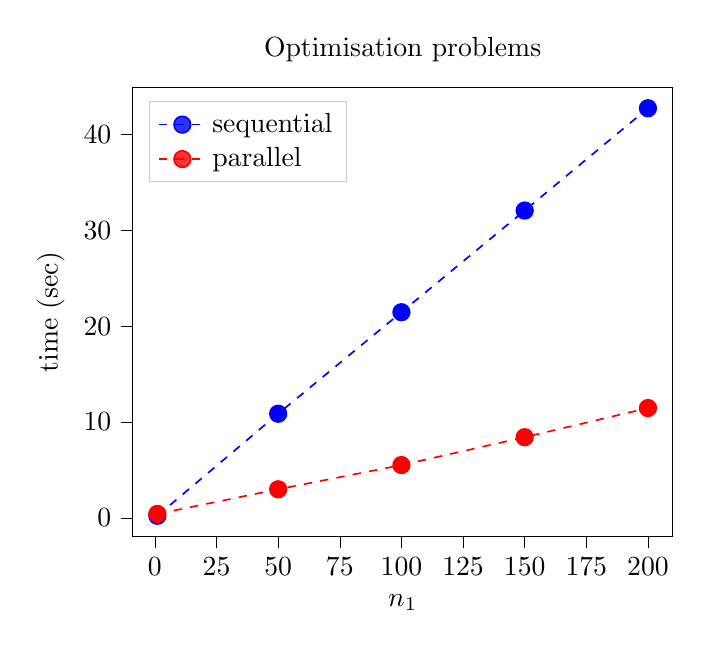
\begin{tikzpicture}

\begin{axis}[
legend cell align={left},
legend style={
  fill opacity=0.8,
  draw opacity=1,
  text opacity=1,
  at={(0.03,0.97)},
  anchor=north west,
  draw=white!80!black
},
tick align=outside,
tick pos=left,
title={Optimisation problems},
x grid style={white!69.0196078431373!black},
xlabel={\(\displaystyle n_1\)},
xmin=-8.95, xmax=209.95,
xtick style={color=black},
xtick={-25,0,25,50,75,100,125,150,175,200,225},
xticklabels={
  \(\displaystyle {\ensuremath{-}25}\),
  \(\displaystyle {0}\),
  \(\displaystyle {25}\),
  \(\displaystyle {50}\),
  \(\displaystyle {75}\),
  \(\displaystyle {100}\),
  \(\displaystyle {125}\),
  \(\displaystyle {150}\),
  \(\displaystyle {175}\),
  \(\displaystyle {200}\),
  \(\displaystyle {225}\)
},
y grid style={white!69.0196078431373!black},
ylabel={time (sec)},
ymin=-1.91896843149916, ymax=44.8788451695003,
ytick style={color=black},
ytick={-10,0,10,20,30,40,50},
yticklabels={
  \(\displaystyle {\ensuremath{-}10}\),
  \(\displaystyle {0}\),
  \(\displaystyle {10}\),
  \(\displaystyle {20}\),
  \(\displaystyle {30}\),
  \(\displaystyle {40}\),
  \(\displaystyle {50}\)
}
]
\addplot [semithick, blue, dashed, mark=*, mark size=3, mark options={solid}]
table {%
1 0.208204914000817
50 10.8651014509996
100 21.4615424589974
150 32.0731122189973
200 42.7516718240004
};
\addlegendentry{sequential}
\addplot [semithick, red, dashed, mark=*, mark size=3, mark options={solid}]
table {%
1 0.408692035001877
50 2.97865102099968
100 5.50569359699875
150 8.41258640300293
200 11.4589973489965
};
\addlegendentry{parallel}
\end{axis}

\end{tikzpicture}

    }
    \resizebox{.49\columnwidth}{!}{%
      % This file was created with tikzplotlib v0.9.12.
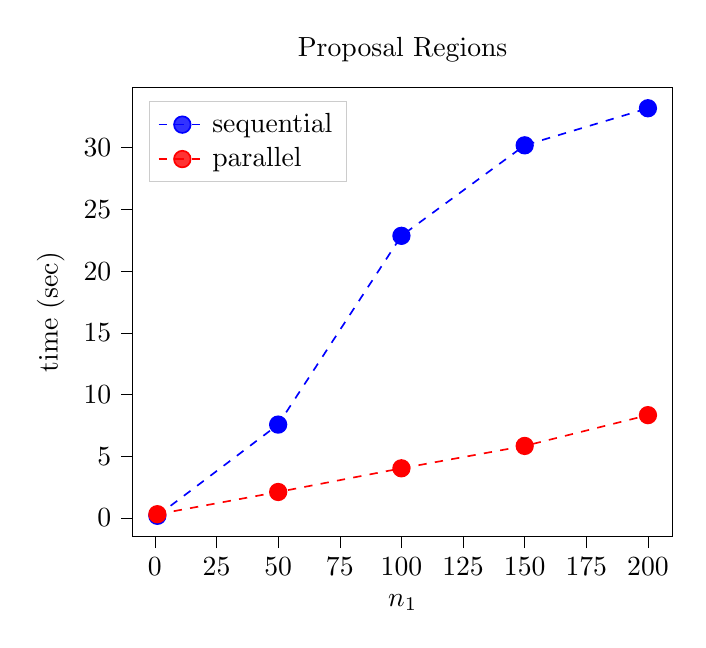
\begin{tikzpicture}

\begin{axis}[
legend cell align={left},
legend style={
  fill opacity=0.8,
  draw opacity=1,
  text opacity=1,
  at={(0.03,0.97)},
  anchor=north west,
  draw=white!80!black
},
tick align=outside,
tick pos=left,
title={Proposal Regions},
x grid style={white!69.0196078431373!black},
xlabel={\(\displaystyle n_1\)},
xmin=-8.95, xmax=209.95,
xtick style={color=black},
xtick={-25,0,25,50,75,100,125,150,175,200,225},
xticklabels={
  \(\displaystyle {\ensuremath{-}25}\),
  \(\displaystyle {0}\),
  \(\displaystyle {25}\),
  \(\displaystyle {50}\),
  \(\displaystyle {75}\),
  \(\displaystyle {100}\),
  \(\displaystyle {125}\),
  \(\displaystyle {150}\),
  \(\displaystyle {175}\),
  \(\displaystyle {200}\),
  \(\displaystyle {225}\)
},
y grid style={white!69.0196078431373!black},
ylabel={time (sec)},
ymin=-1.47990220475122, ymax=34.8494330737497,
ytick style={color=black},
ytick={-5,0,5,10,15,20,25,30,35},
yticklabels={
  \(\displaystyle {\ensuremath{-}5}\),
  \(\displaystyle {0}\),
  \(\displaystyle {5}\),
  \(\displaystyle {10}\),
  \(\displaystyle {15}\),
  \(\displaystyle {20}\),
  \(\displaystyle {25}\),
  \(\displaystyle {30}\),
  \(\displaystyle {35}\)
}
]
\addplot [semithick, blue, dashed, mark=*, mark size=3, mark options={solid}]
table {%
1 0.171431216998826
50 7.56389227700129
100 22.8604871030002
150 30.1939629690005
200 33.1980996519997
};
\addlegendentry{sequential}
\addplot [semithick, red, dashed, mark=*, mark size=3, mark options={solid}]
table {%
1 0.302879205999488
50 2.10327162099929
100 4.02120551399821
150 5.83422652400077
200 8.32964255699881
};
\addlegendentry{parallel}
\end{axis}

\end{tikzpicture}

    }
    \end{center}
    \caption[Execution time exploiting parallelisation]{Comparison
      between parallel and sequential execution of ROMC. We observe
      that the parallel version runs almost 5 times faster.}
      \label{fig:exec_parallel}
\end{figure}
